\documentclass[11pt]{book}
\oddsidemargin 0in
\evensidemargin 0in
\marginparwidth 0in
\textheight 8in
\textwidth 6.5in
\topmargin 0in
\headheight 14pt
\usepackage{amssymb,amsmath,amsthm,fancyhdr,supertabular,longtable,hhline,mathtools}
\usepackage{colortbl}
\usepackage{import, multicol,boxedminipage}
\usepackage{chapterfolder}
\usepackage[metapost,truebbox]{mfpic}
\usepackage[pdflatex]{graphicx}
\usepackage{makeidx}
\usepackage[colorlinks, hyperindex, plainpages=false, linkcolor=blue, urlcolor=blue, pdfpagelabels]{hyperref}
\usepackage[all]{hypcap}
\definecolor{ResultColor}{gray}{0.9}
\theoremstyle{definition}  % this prevents the text in definitions, theorems, and corollaries from being italicized
\newtheorem{defn}{\bf Definition}[chapter]
\newtheorem{thm}{\bf Theorem}[chapter]
\newtheorem{cor}[thm]{\bf Corollary}
\newtheorem{eqn}{\bf Equation}[chapter]
\newtheorem{ex}{\bf Example}[section]
\newtheorem{fig}{\bf Figure}[chapter]
\setlength{\parindent}{0in}
\newcommand{\bbm}{\begin{boxedminipage}{6.41in}}
\newcommand{\ebm}{\end{boxedminipage}}
\usepackage{array}
\setlength{\extrarowheight}{2pt}
\allowdisplaybreaks[2]
\usepackage{cancel}
\usepackage{sectsty}
%\usepackage{appendix}
\usepackage{textcomp}
\usepackage{multirow}
\usepackage[nottoc]{tocbibind}

\DeclareSymbolFont{AMSb}{U}{msb}{m}{n}
\DeclareMathSymbol{\C}{\mathbin}{AMSb}{"43}
\DeclareMathSymbol{\N}{\mathbin}{AMSb}{"4E}
\DeclareMathSymbol{\I}{\mathbin}{AMSb}{"5A}
\DeclareMathSymbol{\Q}{\mathbin}{AMSb}{"51}
\DeclareMathSymbol{\R}{\mathbin}{AMSb}{"52}
\DeclareMathSymbol{\W}{\mathbin}{AMSb}{"57}

\allsectionsfont{\mdseries \scshape}
\makeatletter
\renewcommand\l@section{\@dottedtocline{1}{1.5em}{3em}}
\renewcommand\l@subsection{\@dottedtocline{2}{4.5em}{3.5em}}
\makeatother
\pagestyle{fancy}
\newcounter{HW}
\newcounter{HWindent}

\renewcommand{\textinterrobang}{$! \! \! ?$}

%Below is for Iowna Font
%\renewcommand*\sfdefault{iwona}
%\usepackage[math]{iwona}

%Below is for Helvetica (scaled): 
\usepackage[scaled=.92]{helvet}   
\renewcommand{\familydefault}{\sfdefault}  %makes the text of the book sans serif
\usepackage[helvet]{sfmath}  %makes the math in the book sans serif
\allsectionsfont{\sffamily}  %makes the chapter and section titles sans serif

\makeatletter
\newcases{mycases}{\quad}{%
  \hfil$\m@th\displaystyle{##}$}{$\m@th\displaystyle{##}$\hfil}{\lbrace}{.}
\makeatother

\begin{document}

\renewcommand{\textinterrobang}{$! \! \! ?$}

\chapter{\sc Analytical Trigonometry}

\section{The Pythagorean Identities}

\mfpicnumber{1}

\opengraphsfile{FundamentalTrigonometricIdentities}

\setcounter{footnote}{0}

\label{FundamentalTrigonometricIdentities}

\smallskip

In section Section \ref{TheOtherCircularFunctions}, we first encountered the concept of an \textbf{identity} when discussing Theorem \ref{recipquotid}.   Recall that an identity is an equation which is true regardless of the choice of variable.  Identities are important in mathematics because they facilitate changing forms.\footnote{We've seen the utility of changing form throughout the text, most recently when we completed the square in Chapter \ref{TheConicSections} to put general quadratic equations into standard form in order to graph them.}

\smallskip

We take a moment to generalize Theorem \ref{recipquotid} below. 
\smallskip


\colorbox{ResultColor}{\bbm

\begin{thm} \label{recipquotidfull}  \textbf{Reciprocal and Quotient Identities:} \index{Reciprocal Identities} \index{Quotient Identities}  The following relationships hold for all angles $\theta$ provided each side of each equation is defined.

\begin{multicols}{4}

\begin{itemize}

\item $\sec(\theta) = \dfrac{1}{\cos(\theta)}$ 

\item $\cos(\theta) = \dfrac{1}{\sec(\theta)}$

\item $\csc(\theta) = \dfrac{1}{\sin(\theta)}$

\item $\sin(\theta) = \dfrac{1}{\csc(\theta)}$

\end{itemize}

\end{multicols}


\begin{multicols}{4}

\begin{itemize}

\item $\tan(\theta) = \dfrac{\sin(\theta)}{\cos(\theta)}$

\item $\cot(\theta) = \dfrac{\cos(\theta)}{\sin(\theta)}$

\item $\cot(\theta) = \dfrac{1}{\tan(\theta)}$

\item $\tan(\theta) = \dfrac{1}{\cot(\theta)}$

\end{itemize}

\end{multicols}

\smallskip

\end{thm}

\ebm}

\smallskip

It is important to remember that the equivalences stated in Theorem \ref{recipquotidfull}  are valid only when \textit{all} quantities described therein are defined.  As an example, $\tan(0) = 0$, but $\tan(0) \neq \frac{1}{\cot(0)}$ since $\cot(0)$ is undefined.

\smallskip

When it comes down to it, the Reciprocal and Quotient Identities amount to giving different ratios on the Unit Circle different names.  The main focus of this section is on a more algebraic relationship between certain pairs of the circular functions: the \index{Pythagorean Identities}\index{Identities ! Pythagorean}\textbf{Pythagorean Identities}.

\smallskip

Recall in Definition \ref{sinecosineunitcircledefn}, the cosine and sine of an angle is defined as the $x$ and $y$-coordinate, respectively, of a point on the Unit Circle.  Since the coordinates of all points $(x,y)$ on the Unit Circle satisfy the equation $x^2+y^2 = 1$, we get for all angles $\theta$, $\left(\cos(\theta)\right)^2 + \left(\sin(\theta)\right)^2 = 1$.  An unfortunate\footnote{This is unfortunate from a `function notation' perspective. See Section \ref{TheInverseTrigonometricFunctions}.} convention, which the authors are compelled to perpetuate,  is to write $\left(\cos(\theta)\right)^2$ as $\cos^{2}(\theta)$ and $\left(\sin(\theta)\right)^2$ as $\sin^{2}(\theta)$. Rewriting the identity using this convention results in the following theorem, which is without a doubt one of the most important results in Trigonometry.

\smallskip

\colorbox{ResultColor}{\bbm

\begin{thm} \label{cosinesinepythid} \textbf{The Pythagorean Identity:}  For any angle $\theta$, $\cos^{2}(\theta) + \sin^{2}(\theta) = 1$.

\end{thm}

\ebm} 

\smallskip

The moniker `Pythagorean' brings to mind the Pythagorean Theorem, from which both the Distance Formula and the equation for a circle are ultimately derived.\footnote{See Sections \ref{AppCartesianPlane} and \ref{Circles} for details.}  The word `Identity' reminds us that, regardless of the angle $\theta$, the equation in Theorem \ref{cosinesinepythid} is always true.  

\smallskip

If one of $\cos(\theta)$ or $\sin(\theta)$ is known, Theorem \ref{cosinesinepythid} can be used to determine the other, up to a ($\pm$) sign.  If, in addition, we know where the terminal side of $\theta$ lies when in standard position, then we can remove the ambiguity of the ($\pm$) and completely determine the missing value.\footnote{See the illustration following Example \ref{circularfunctionsex} to refresh yourself which circular functions are positive in which quadrants.}  We illustrate this approach in the following example.


\smallskip

\begin{ex} \label{cosinesinepythidex} Use Theorem \ref{cosinesinepythid} and the given information  to find the indicated value.
\begin{enumerate}

\item If $\theta$ is a Quadrant II angle with  $\sin(\theta) = \frac{3}{5}$, find $\cos(\theta)$.

\item If $\pi < t < \frac{3\pi}{2}$ with  $\cos(t) = -\frac{\sqrt{5}}{5}$, find $\sin(t)$.

\item  If $\sin(\theta) = 1$, find $\cos(\theta)$.

\end{enumerate}



{\bf Solution.}  \begin{enumerate} \item  When we substitute $\sin(\theta) = \frac{3}{5}$ into The Pythagorean Identity, $\cos^{2}(\theta) + \sin^{2}(\theta) = 1$, we obtain $\cos^{2}(\theta) + \frac{9}{25} = 1$.  Solving, we find $\cos(\theta) = \pm \frac{4}{5}$.  Since $\theta$ is a Quadrant II angle, we know $\cos(\theta)<0$.  Hence, we select  $\cos(\theta) = - \frac{4}{5}$.

\item Here we're using the variable $t$ instead $\theta$ which usually corresponds to a real number variable instead of an angle.  As usual,  we associate real numbers $t$ with angles $\theta$ measuring $t$ radians,\footnote{See page \pageref{wrappingfunction} if you need a review of how we associate real numbers with angles in radian measure.} so the the Pythagorean Identity works equally well for all real numbers $t$ as it does for all angles $\theta$.

\smallskip

 Substituting $\cos(t) = -\frac{\sqrt{5}}{5}$ into $\cos^{2}(t) + \sin^{2}(t) = 1$ gives $\sin(t) = \pm \frac{2}{\sqrt{5}} = \pm \frac{2 \sqrt{5}}{5}$.  Since  $\pi < t < \frac{3\pi}{2}$, we know $t$ corresponds to a Quadrant III angle, so $\sin(t) <0$.   Hence,  $\sin(t) = -\frac{2 \sqrt{5}}{5}$.

\item  When we substitute $\sin(\theta) = 1$ into $\cos^{2}(\theta) + \sin^{2}(\theta) = 1$, we find $\cos(\theta) = 0$. \qed 

\end{enumerate}

\end{ex}

\smallskip

The reader is encouraged to compare and contrast the solution strategies demonstrated in Example \ref{cosinesinepythidex} with those showcases in Examples \ref{advancedrefangleex} and \ref{cosinesinecircleex} in Section \ref{TheCircularFunctionsSineandCosine}.  

\smallskip

As with many tools in mathematics, identities give us a different way to approach and solve problems.\footnote{For example, factoring, completing the square, and the quadratic formula are three different (yet equivalent) ways to solve a quadratic equation.  See Section \ref{AppQuadEqus} for a refresher.}  As always, the key is to determine which approach makes the most sense (is more efficient, for instance) in the given scenario.  

\smallskip


Our next task is to use use the Reciprocal and Quotient Identities found in Theorem \ref{recipquotidfull} coupled with the Pythagorean Identity found in Theorem \ref{cosinesinepythid} to derive new Pythagorean-like identities for the remaining four circular functions.   

\smallskip

Assuming $\cos(\theta) \neq 0$, we may start with $\cos^{2}(\theta) + \sin^{2}(\theta) = 1$ and divide both sides by $\cos^{2}(\theta)$ to obtain $1 + \frac{\sin^{2}(\theta)}{\cos^{2}(\theta)} = \frac{1}{\cos^{2}(\theta)}$.  Using properties of exponents along with the Reciprocal and Quotient Identities, this reduces to $1 + \tan^{2}(\theta) = \sec^{2}(\theta)$. 

\smallskip

 If $\sin(\theta) \neq 0$, we can divide both sides of the identity $\cos^{2}(\theta) + \sin^{2}(\theta) = 1$ by $\sin^{2}(\theta)$, apply Theorem \ref{recipquotidfull} once again,  and obtain $\cot^{2}(\theta) + 1 = \csc^{2}(\theta)$.  
 
 \smallskip
 
 These three Pythagorean Identities are worth memorizing and they, along with some of their other common forms, are summarized in the following theorem.

\smallskip

\colorbox{ResultColor}{\bbm

\begin{thm} \label{pythids}  \textbf{The Pythagorean Identities:} \index{Pythagorean Identities}

\begin{enumerate}

\item $\cos^{2}(\theta) + \sin^{2}(\theta) = 1$.

\textbf{Common Alternate Forms:}

\begin{itemize}

\item  $1 - \sin^{2}(\theta) = \cos^{2}(\theta)$

\item  $1 - \cos^{2}(\theta) = \sin^{2}(\theta)$

\end{itemize}

\item $1 + \tan^{2}(\theta) = \sec^{2}(\theta)$, provided $\cos(\theta) \neq 0$.

\textbf{Common Alternate Forms:}

\begin{itemize}

\item  $\sec^{2}(\theta) - \tan^{2}(\theta) = 1$

\item  $\sec^{2}(\theta) - 1 = \tan^{2}(\theta)$

\end{itemize}

\item $1 + \cot^{2}(\theta) = \csc^{2}(\theta)$, provided $\sin(\theta) \neq 0$.

\textbf{Common Alternate Forms:}

\begin{itemize}

\item  $\csc^{2}(\theta) - \cot^{2}(\theta) = 1$

\item  $\csc^{2}(\theta) - 1 = \cot^{2}(\theta)$

\end{itemize}

\end{enumerate}

\smallskip

\end{thm}

\ebm}

\smallskip

As usual, the formulas states in Theorem \ref{pythids} work equally well for (the applicable) angles as well as real numbers.

\smallskip

\begin{ex} \label{usingidtofindvaluesex1}  Use Theorems \ref{recipquotidfull}   and \ref{pythids}  to find the indicated values.

\begin{enumerate}

\item  If $\theta$ is a Quadrant IV angle with $\sec(\theta) = 3$, find $\tan(\theta)$.

\item   Find $\csc(t)$ if  $\pi < t < \frac{3\pi}{2}$ and $\cot(t) = 2$.

\item  If $\theta$ is a Quadrant II angle with $\cos(\theta) = -\frac{3}{5}$, find the exact values of the remaining circular functions.

\end{enumerate}

{\bf Solution.}

\begin{enumerate}

\item  Per Theorem  \ref{pythids}, $\tan^{2}(\theta) = \sec^{2}(\theta) -1$.  Since  $\sec(\theta) = 3$, we have $\tan^{2}(\theta) = (3)^2 - 1 = 8$, or  $\tan(\theta) = \pm \sqrt{8} = \pm 2 \sqrt{2}$. Since $\theta$ is a Quadrant IV angle, we know $\tan(\theta) < 0$ so $\tan(\theta) = -2\sqrt{2}$.

\item  Again, using Theorem  \ref{pythids}, we have $\csc^{2}(t) = 1 + \cot^{2}(t)$, so we have $\csc^{2}(t) = 1 + (2)^2 = 5$.  This gives $\csc(t) = \pm \sqrt{5}$.  Since $\pi < t < \frac{3\pi}{2}$, $t$ corresponds to   a Quadrant III angle, so $\csc(t) = -\sqrt{5}$.

\item  With five function values to find, we have our work cut out for us.  From Theorem \ref{recipquotidfull}, we know $\sec(\theta) = \frac{1}{\cos(\theta)}$, so we (quickly) get $\sec(\theta) = \frac{1}{-3/5} = - \frac{5}{3}$.  

\smallskip

Next, we go after $\sin(\theta)$  since between $\sin(\theta)$ and  $\cos(\theta)$, we can get all of the remaining values courtesy of Theorem \ref{recipquotidfull}. 

\smallskip

 From Theorem \ref{pythids}, we  have $\sin^{2}(\theta) = 1 - \cos^{2}(\theta)$,  so $\sin^{2}(\theta) = 1 - \left(\frac{3}{5}\right)^2 = 1 - \frac{9}{25} = \frac{16}{25}$.  Hence,  $\sin(\theta) = \pm \frac{4}{5}$ but since $\theta$ is a Quadrant II angle, we select $\sin(\theta) = \frac{4}{5}$.
 
 \smallskip
 
Back to  Theorem \ref{recipquotidfull}, we get $\csc(\theta) = \frac{1}{\sin(\theta)} = \frac{1}{4/5} = \frac{5}{4}$, $\tan(\theta) = \frac{\sin(\theta)}{\cos(\theta)} = \frac{4/5}{-3/5} = -\frac{4}{3}$, and $\cot(\theta) = \frac{\cos(\theta)}{\sin(\theta)} = \frac{-3/5}{4/5} = -\frac{3}{4}$.  \qed 


\end{enumerate}



\end{ex}


\smallskip

Again, the reader is encouraged to study the solution methodology illustrated in  Example \ref{usingidtofindvaluesex1} as compared with that employed in Example \ref{circularfunctionscircleex} in Section \ref{TheOtherCircularFunctions}.

\smallskip

Trigonometric identities play an important role in not just Trigonometry, but in Calculus as well.  We'll use them in this book to find the values of the circular functions of an angle and solve equations and inequalities.  In Calculus, they are needed to simplify otherwise complicated expressions.  In the next example, we make good use of the Theorems \ref{recipquotidfull} and \ref{pythids}.

\begin{ex} \label{idornotex1} Verify the following identities. Assume that all quantities are defined.

\begin{multicols}{2}

\begin{enumerate}

\item  $\tan(\theta) = \sin(\theta) \sec(\theta)$

\item  $(\tan(t) - \sec(t)) (\tan(t) + \sec(t))  = -1$

\setcounter{HW}{\value{enumi}}

\end{enumerate}

\end{multicols}

\begin{multicols}{2}

\begin{enumerate}

\setcounter{enumi}{\value{HW}}

\item  $\sin^{2}(x) \cos^{3}(x) = \sin^{2}(x) \left(1 - \sin^{2}(x)\right) \cos(x)$ \vphantom{$\dfrac{\sec(x)}{1 - \tan(x)}$}

\item  $\dfrac{\sec(t)}{1 - \tan(t)} = \dfrac{1}{\cos(t) - \sin(t)}$

\setcounter{HW}{\value{enumi}}

\end{enumerate}

\end{multicols}

\begin{multicols}{2}

\begin{enumerate}

\setcounter{enumi}{\value{HW}}

\item  $6\sec(x) \tan(x) = \dfrac{3}{1-\sin(x)} - \dfrac{3}{1 + \sin(x)}$

\item  \label{pythconjex} $\dfrac{\sin(\theta)}{1 - \cos(\theta)} = \dfrac{1 + \cos(\theta)}{\sin(\theta)}$

\end{enumerate}

\end{multicols}

{\bf Solution.}  In verifying identities, we typically start with the more complicated side of the equation and use known identities to \textit{transform} it into the other side of the equation. 

\begin{enumerate} 


\item Starting with the right hand side of $\tan(\theta) = \sin(\theta) \sec(\theta)$, we use $\sec(\theta) = \frac{1}{\cos(\theta)}$ and find:  \[ \sin(\theta) \sec(\theta) = \sin(\theta) \dfrac{1}{\cos(\theta)} = \dfrac{\sin(\theta)}{\cos(\theta)} = \tan(\theta),\]

where the last equality is courtesy of Theorem \ref{recipquotidfull}.

\item Expanding the left hand side, we get:  $(\tan(t) - \sec(t)) (\tan(t) + \sec(t)) = \tan^{2}(t) - \sec^{2}(t)$.  From Theorem \ref{pythids}, we know  $\sec^{2}(t) - \tan^{2}(t) = 1$, which isn't \textit{quite} what we have. We are off by a negative sign ($-$),  so we factor it out:

\[ (\tan(t) - \sec(t)) (\tan(t) + \sec(t)) = \tan^{2}(t) - \sec^{2}(t) = (-1)( \sec^{2}(t) - \tan^{2}(t)) = (-1)(1) = -1.\]

\item  Starting with the right hand side,\footnote{We hope by this point a shift of variable to `$x$' instead of `$\theta$' or `$t$' is a non-issue.} we notice we have a quantity we can immediately simplify per Theorem \ref{pythids}:  $1 - \sin^{2}(x) = \cos^{2}(x)$ .  This increases the number of factors of cosine, (which is part of our goal in looking at the left hand side), so we proceed:

\[ \sin^{2}(x) \left(1 - \sin^{2}(x)\right) \cos(x) = \sin^{2}(x) \cos^{2}(x) \cos(x) = \sin^{2}(x) \cos^{3}(x).\]

\item  While both sides of our next identity contain fractions, the left side affords us more opportunities to use our identities.\footnote{Or, to put to another way, earn more partial credit if this were an exam question!} Substituting $\sec(t) = \frac{1}{\cos(t)}$ and $\tan(t) = \frac{\sin(t)}{\cos(t)}$, we get:


\[ \begin{array}{rcl} \dfrac{\sec(t)}{1 - \tan(t)} & = & \dfrac{ \dfrac{1}{\cos(t)}}{1 - \dfrac{\sin(t)}{\cos(t)}} = \dfrac{ \dfrac{1}{\cos(t)}}{1 - \dfrac{\sin(t)}{\cos(t)}} \cdot \dfrac{\cos(t)}{\cos(t)} \\ [.4in]
 & = & \dfrac{\left( \dfrac{1}{\cos(t)} \right) ( \cos(t) )}{\left(1 - \dfrac{\sin(t)}{\cos(t)}\right)(\cos(t))} = \dfrac{1}{(1)(\cos(t)) - \left(\dfrac{\sin(t)}{\cos(t)}\right)(\cos(t))} \\ [.4in]
                                                           & = & \dfrac{1}{\cos(t) - \sin(t)}, \end{array} \]
which is exactly what we had set out to show.  

\item Starting with the right hand side, we can get started by obtaining common denominators to add:

\[ \begin{array}{rcl}

\dfrac{3}{1-\sin(x)} - \dfrac{3}{1 + \sin(x)} & = & \dfrac{3(1 + \sin(x))}{(1-\sin(x))(1 + \sin(x))} - \dfrac{3(1-\sin(x))}{(1 + \sin(x))(1-\sin(x))} \\ [.25in]
                                                        & = & \dfrac{3 + 3\sin(x)}{1 - \sin^{2}(x)} - \dfrac{3 - 3\sin(x)}{1 - \sin^{2}(x)} \\ [.25in]
                                                        & = & \dfrac{(3 + 3\sin(x)) - (3 - 3\sin(x))}{1 - \sin^{2}(x)} \\ [.25in]                                                        																																	
                                                        & = & \dfrac{6 \sin(x)}{1 - \sin^{2}(x)} \end{array} \]

At this point, we have at least reduced the number of fractions from two to one, it may not be clear how to proceed.   When this happens, it isn't a bad idea to start working with the other side of the identity to get some clues how to proceed.

\smallskip

Using a reciprocal and quotient identity, we find $6\sec(x) \tan(x) = 6 \left(\frac{1}{\cos(x)}\right) \left(\frac{\sin(x)}{\cos(x)}\right) = \frac{6 \sin(x)}{\cos^{2}(x)}$.  

\smallskip

Theorem \ref{pythids} tells us $1 -  \sin^{2}(x) = \cos^{2}(x)$, which means to our surprise and delight, we are much closer to our goal that we may have originally thought:

\[ \begin{array}{rcl}

\dfrac{3}{1-\sin(x)} - \dfrac{3}{1 + \sin(x)} & = & \dfrac{6 \sin(x)}{1 - \sin^{2}(x)}= \dfrac{6 \sin(x)}{\cos^{2}(x)} \\ [.25in]
& = &  6 \left(\dfrac{1}{\cos(x)}\right)\left( \dfrac{\sin(x)}{\cos(x)}\right) = 6 \sec(x) \tan(x). \\ \end{array} \]

\item  It is debatable which side of the identity is more complicated.  One thing which stands out is that the denominator on the left hand side is $1-\cos(\theta)$, while the numerator of the right hand side is $1+\cos(\theta)$.  This suggests the strategy of starting with the left hand side and multiplying the numerator and denominator by the quantity $1+\cos(\theta)$.   Theorem \ref{pythids} comes to our aid once more when we simplify $1-\cos^{2}(\theta) = \sin^{2}(\theta)$:

\[ \begin{array}{rcl}


\dfrac{\sin(\theta)}{1 - \cos(\theta)} & = & \dfrac{\sin(\theta)}{(1 - \cos(\theta))} \cdot \dfrac{(1 + \cos(\theta))}{(1 + \cos(\theta))} = \dfrac{\sin(\theta)(1 + \cos(\theta))}{(1 - \cos(\theta))(1 + \cos(\theta))} \\ [.25in]
& = & \dfrac{\sin(\theta)(1 + \cos(\theta))}{1 - \cos^{2}(\theta)} = \dfrac{\sin(\theta)(1 + \cos(\theta))}{\sin^{2}(\theta)} \\ [.25in]
& = & \dfrac{\cancel{\sin(\theta)}(1 + \cos(\theta))}{\cancel{\sin(\theta)}\sin(\theta)} = \dfrac{1 + \cos(\theta)}{\sin(\theta)} \end{array} \]

\vspace{-.1in} \qed

\end{enumerate}

\end{ex}

In Example \ref{idornotex1} number \ref{pythconjex} above,  we see that multiplying  $1-\cos(\theta)$ by $1+\cos(\theta)$ produces a difference of squares that can be simplified to one term using Theorem \ref{pythids}.  

\smallskip

This is exactly the same kind of phenomenon that occurs when we multiply expressions such as $1 - \sqrt{2}$ by $1+\sqrt{2}$ or $3 - 4i$ by $3+4i$. In algebra, these sorts of expressions were called `conjugates.'\footnote{See Sections  \ref{AppCmpNums} and \ref{AppRadEqus}.}  

\smallskip

For this reason, the quantities $(1-\cos(\theta))$ and $(1+\cos(\theta))$ are called `Pythagorean Conjugates.'  Below is a list of other common Pythagorean Conjugates.  

\smallskip

\phantomsection
\label{PythagoreanConjugates}
\smallskip
\colorbox{ResultColor}{\bbm

\smallskip

\centerline{\textbf{Pythagorean Conjugates}}  \index{Pythagorean Conjugates}

\begin{itemize}

\item $1 - \cos(\theta)$ and  $1+\cos(\theta)$:  $(1-\cos(\theta))(1+\cos(\theta)) = 1 - \cos^{2}(\theta) = \sin^{2}(\theta)$

\item  $1-\sin(\theta)$ and $1 + \sin(\theta)$:  $(1-\sin(\theta))(1+\sin(\theta)) = 1 - \sin^{2}(\theta) = \cos^{2}(\theta)$

\item  $\sec(\theta)-1$ and $\sec(\theta)+1$:  $(\sec(\theta)-1)(\sec(\theta)+1) = \sec^{2}(\theta) - 1 =  \tan^{2}(\theta)$

\item  $\sec(\theta)-\tan(\theta)$ and $\sec(\theta)+\tan(\theta)$:  $(\sec(\theta)-\tan(\theta))(\sec(\theta)+\tan(\theta)) = \sec^{2}(\theta) - \tan^{2}(\theta) = 1$

\item  $\csc(\theta)-1$ and $\csc(\theta)+1$:  $(\csc(\theta)-1)(\csc(\theta)+1) = \csc^{2}(\theta) - 1 =  \cot^{2}(\theta)$

\item  $\csc(\theta)-\cot(\theta)$ and $\csc(\theta)+\cot(\theta)$:  $(\csc(\theta)-\cot(\theta))(\csc(\theta)+\cot(\theta)) = \csc^{2}(\theta) - \cot^{2}(\theta) = 1$

\smallskip

\end{itemize}

\ebm}


\smallskip

Verifying trigonometric identities requires a healthy mix of tenacity and inspiration.  You will need to spend many hours struggling with them just to become proficient in the basics. 

\smallskip

 Like many things in life, there is no short-cut here -- there is no complete algorithm for verifying identities.  Nevertheless, a summary of some strategies which  may be helpful (depending on the situation) is provided below and ample practice is provided for you in the Exercises.
 
 \smallskip

\phantomsection
\label{IdentityHelp}

\colorbox{ResultColor}{\bbm

\medskip

\centerline{\textbf{Strategies for Verifying Identities}} 

\begin{itemize}

\item  Try working on the more complicated side of the identity.

\item Use the Reciprocal and Quotient Identities in Theorem \ref{recipquotidfull} to write functions on one side of the identity in terms of the functions on the other side of the identity.  

\smallskip

Simplify the resulting complex fractions.

\item Add rational expressions with unlike denominators by obtaining common denominators.

\item  Use the Pythagorean Identities in Theorem \ref{pythids} to `exchange' sines and cosines, secants and tangents, cosecants and cotangents, and simplify sums or differences of squares to one term. 

\item Multiply numerator \textbf{and} denominator by Pythagorean
Conjugates in order to take advantage of the Pythagorean Identities in  Theorem \ref{pythids}.

\item If you find yourself stuck working with one side of the identity, try starting with the other side of the identity and see if you can find a way to bridge the two parts of your work.

\item  Try \textit{something}.  The more you work with identities, the better you'll get with identities.

\smallskip


\end{itemize}

\ebm}

\newpage

\subsection{Exercises}


In Exercises \ref{useidsforvaluesfirst01} - \ref{useidsforvalueslast01}, use the Reciprocal and Quotient Identities (Theorem \ref{recipquotidfull}) along with the Pythagorean Identities (Theorem \ref{pythids}), to find the value of the circular function requested below. (Find the exact value unless otherwise indicated.)

\begin{multicols}{3}
\begin{enumerate}

\item  \label{useidsforvaluesfirst01}  If  $\sin(\theta) = \frac{\sqrt{5}}{5}$, find $\csc(\theta)$.

\item  If $\sec(\theta) = - 4$,  find $\cos(\theta)$.

\item  If $\tan(t) = 3$, find $\cot(t)$.

\setcounter{HW}{\value{enumi}}
\end{enumerate}
\end{multicols}

\begin{enumerate}

\setcounter{enumi}{\value{HW}}

\item  If $\theta$ is a Quadrant IV angle with $\cos(\theta) = \frac{5}{13}$, find $\sin(\theta)$.

\item  If $\theta$ is a Quadrant III angle with $\tan(\theta) = 2$, find $\sec(\theta)$.

\item  If $\frac{\pi}{2} < t < \pi$ with $\cot(t) = -2$, find $\csc(t)$.

\item  If $\sec(\theta) = 3$ and $\sin(\theta) < 0$, find $\tan(\theta)$.

\item If $\sin(\theta) = -\frac{2}{3}$ but $\tan(\theta) > 0$, find $\cos(\theta)$.

\item If $0 < t < \frac{\pi}{2}$ and $\sin(t) = 0.42$, find $\cos(t)$, rounded to four decimal places.

\item  If $\theta$ is Quadrant IV angle with $\sec(\theta) = 1.17$, find $\tan(\theta)$, rounded to four decimal places.

\item  \label{useidsforvalueslast01}  If $\pi < t < \frac{3\pi}{2}$ with $\cot(t) = 4.2$, find $\csc(t)$, rounded to four decimal places.

\setcounter{HW}{\value{enumi}}
\end{enumerate}

In Exercises \ref{useidsforvaluesfirst02} - \ref{useidsforvalueslast02}, use the Reciprocal and Quotient Identities (Theorem \ref{recipquotidfull}) along with the Pythagorean Identities (Theorem \ref{pythids}), to find the exact values of the remaining circular functions.  (Compare your methods with how you solved Exercises \ref{findothercircfirst} - \ref{findothercirclast} in Section \ref{TheOtherCircularFunctions}.)


\begin{multicols}{2}

\begin{enumerate}


\setcounter{enumi}{\value{HW}}

\item $\sin(\theta) = \dfrac{3}{5}$ with $\theta$ in Quadrant II \label{useidsforvaluesfirst02}
\item $\tan(\theta) = \dfrac{12}{5}$ with $\theta$ in Quadrant III

\setcounter{HW}{\value{enumi}}

\end{enumerate}

\end{multicols}

\begin{multicols}{2}

\begin{enumerate}

\setcounter{enumi}{\value{HW}}

\item $\csc(\theta) = \dfrac{25}{24}$ with $\theta$ in Quadrant I
\item $\sec(\theta) = 7$ with $\theta$ in Quadrant IV \vphantom{$\dfrac{25}{24}$}

\setcounter{HW}{\value{enumi}}

\end{enumerate}

\end{multicols}

\begin{multicols}{2}

\begin{enumerate}

\setcounter{enumi}{\value{HW}}

\item $\csc(\theta) = -\dfrac{10\sqrt{91}}{91}$ with $\theta$ in Quadrant III
\item $\cot(\theta) = -23$ with $\theta$ in Quadrant II \vphantom{$\dfrac{10}{\sqrt{91}}$}

\setcounter{HW}{\value{enumi}}

\end{enumerate}

\end{multicols}

\begin{multicols}{2}

\begin{enumerate}

\setcounter{enumi}{\value{HW}}

\item  $\tan(\theta) = -2$ with $\theta$ in Quadrant IV.
\item  $\sec(\theta) = -4$ with $\theta$ in Quadrant II.

\setcounter{HW}{\value{enumi}}

\end{enumerate}

\end{multicols}

\begin{multicols}{2}

\begin{enumerate}

\setcounter{enumi}{\value{HW}}

\item $\cot(\theta) = \sqrt{5}$ with $\theta$ in Quadrant III. \vphantom{$\dfrac{25}{24}$}
\item  $\cos(\theta) = \dfrac{1}{3}$ with $\theta$ in Quadrant I.

\setcounter{HW}{\value{enumi}}

\end{enumerate}

\end{multicols}

\begin{multicols}{2}

\begin{enumerate}

\setcounter{enumi}{\value{HW}}

\item  $\cot(t) = 2$ with $0  < t < \dfrac{\pi}{2}$.
\item  $\csc(t) = 5$ with $\dfrac{\pi}{2} < t < \pi$.

\setcounter{HW}{\value{enumi}}

\end{enumerate}

\end{multicols}

\begin{multicols}{2}

\begin{enumerate}

\setcounter{enumi}{\value{HW}}

\item  $\tan(t) = \sqrt{10}$ with $\pi < t < \dfrac{3\pi}{2}$.
\item  $\sec(t) = 2\sqrt{5}$ with $\dfrac{3\pi}{2} < t < 2\pi$.\label{useidsforvalueslast02}


\setcounter{HW}{\value{enumi}}

\end{enumerate}

\end{multicols}


\begin{enumerate}
\setcounter{enumi}{\value{HW}}

\item Skippy claims  $\cos(\theta) + \sin(\theta) = 1$ is an identity because when $\theta = 0$, the equation is true.  Is Skippy correct? Explain.

\setcounter{HW}{\value{enumi}}
\end{enumerate}

\pagebreak

In Exercises \ref{firstcirciden} - \ref{lastcirciden}, verify the identity.  Assume that all quantities are defined.

\begin{multicols}{2}

\begin{enumerate}

\setcounter{enumi}{\value{HW}}

\item $\cos(\theta) \sec(\theta) = 1$ \label{firstcirciden}
\item $\tan(t)\cos(t) = \sin(t)$

\setcounter{HW}{\value{enumi}}

\end{enumerate}

\end{multicols}

\begin{multicols}{2}

\begin{enumerate}

\setcounter{enumi}{\value{HW}}

\item $\sin(\theta) \csc(\theta) = 1$
\item $\tan(t) \cot(t) = 1$

\setcounter{HW}{\value{enumi}}

\end{enumerate}

\end{multicols}

\begin{multicols}{2}

\begin{enumerate}

\setcounter{enumi}{\value{HW}}

\item $\csc(x) \cos(x) = \cot(x)$ \vphantom{$\dfrac{\sin(x)}{\cos^{2}(x)}$}
\item $\dfrac{\sin(t)}{\cos^{2}(t)} = \sec(t) \tan(t)$

\setcounter{HW}{\value{enumi}}

\end{enumerate}

\end{multicols}

\begin{multicols}{2}

\begin{enumerate}

\setcounter{enumi}{\value{HW}}

\item $\dfrac{\cos(\theta)}{\sin^{2}(\theta)} = \csc(\theta) \cot(\theta)$
\item $\dfrac{1+ \sin(x)}{\cos(x)} = \sec(x) + \tan(x)$

\setcounter{HW}{\value{enumi}}

\end{enumerate}

\end{multicols}

\begin{multicols}{2}

\begin{enumerate}

\setcounter{enumi}{\value{HW}}

\item $\dfrac{1 - \cos(\theta)}{\sin(\theta)} = \csc(\theta) - \cot(\theta)$
\item  $\dfrac{\cos(t)}{1 - \sin^{2}(t)} = \sec(t)$

\setcounter{HW}{\value{enumi}}

\end{enumerate}

\end{multicols}

\begin{multicols}{2}

\begin{enumerate}

\setcounter{enumi}{\value{HW}}

\item  $\dfrac{\sin(x)}{1 - \cos^{2}(x)} = \csc(x)$
\item  $\dfrac{\sec(t)}{1 + \tan^{2}(t)} = \cos(t)$

\setcounter{HW}{\value{enumi}}

\end{enumerate}

\end{multicols}

\begin{multicols}{2}

\begin{enumerate}

\setcounter{enumi}{\value{HW}}

\item  $\dfrac{\csc(\theta)}{1 + \cot^{2}(\theta)} = \sin(\theta)$
\item   $\dfrac{\tan(x)}{\sec^{2}(x) - 1} = \cot(x)$

\setcounter{HW}{\value{enumi}}

\end{enumerate}

\end{multicols}

\begin{multicols}{2}

\begin{enumerate}

\setcounter{enumi}{\value{HW}}

\item   $\dfrac{\cot(t)}{\csc^{2}(t) - 1} = \tan(t)$
\item $4 \cos^{2}(\theta) + 4 \sin^{2}(\theta) = 4$

\setcounter{HW}{\value{enumi}}

\end{enumerate}

\end{multicols}

\begin{multicols}{2}

\begin{enumerate}

\setcounter{enumi}{\value{HW}}

\item $9 - \cos^{2}(t) - \sin^{2}(t) = 8$
\item $\tan^{3}(t) = \tan(t)\sec^{2}(t) - \tan(t)$

\setcounter{HW}{\value{enumi}}

\end{enumerate}

\end{multicols}

\begin{multicols}{2}

\begin{enumerate}

\setcounter{enumi}{\value{HW}}

\item $\sin^{5}(x) = \left(1-\cos^{2}(x)\right)^{2} \sin(x)$
\item $\sec^{10}(t) = \left(1 + \tan^{2}(t)\right)^4 \sec^{2}(t)$

\setcounter{HW}{\value{enumi}}

\end{enumerate}

\end{multicols}

\begin{multicols}{2}

\begin{enumerate}

\setcounter{enumi}{\value{HW}}

\item $\cos^{2}(x)\tan^{3}(x) = \tan(x) - \sin(x)\cos(x)$
\item $\sec^{4}(t) - \sec^{2}(t) = \tan^{2}(t) + \tan^{4}(t)$

\setcounter{HW}{\value{enumi}}

\end{enumerate}

\end{multicols}

\begin{multicols}{2}

\begin{enumerate}

\setcounter{enumi}{\value{HW}}

\item $\dfrac{\cos(\theta) + 1}{\cos(\theta) - 1} = \dfrac{1 + \sec(\theta)}{1 - \sec(\theta)}$
\item $\dfrac{\sin(t) + 1}{\sin(t) - 1} = \dfrac{1 + \csc(t)}{1 - \csc(t)}$

\setcounter{HW}{\value{enumi}}

\end{enumerate}

\end{multicols}

\begin{multicols}{2}

\begin{enumerate}

\setcounter{enumi}{\value{HW}}

\item $\dfrac{1 - \cot(x)}{1+ \cot(x)} = \dfrac{\tan(x) - 1}{\tan(x) + 1}$
\item $\dfrac{1 - \tan(t)}{1+ \tan(t)} = \dfrac{\cos(t) - \sin(t)}{\cos(t) + \sin(t)}$

\setcounter{HW}{\value{enumi}}

\end{enumerate}

\end{multicols}

\begin{multicols}{2}

\begin{enumerate}

\setcounter{enumi}{\value{HW}}

\item $\tan(\theta) + \cot(\theta) = \sec(\theta)\csc(\theta)$
\item $\csc(t) - \sin(t) = \cot(t)\cos(t)$

\setcounter{HW}{\value{enumi}}

\end{enumerate}

\end{multicols}

\begin{multicols}{2}

\begin{enumerate}

\setcounter{enumi}{\value{HW}}

\item $\cos(x) - \sec(x) = -\tan(x)\sin(x)$
\item $\cos(x)(\tan(x) + \cot(x)) = \csc(x)$

\setcounter{HW}{\value{enumi}}

\end{enumerate}

\end{multicols}

\begin{multicols}{2}

\begin{enumerate}

\setcounter{enumi}{\value{HW}}

\item $\sin(t)(\tan(t) + \cot(t)) = \sec(t)$ \vphantom{$\dfrac{1}{1-\cos(t)}$}
\item   $\dfrac{1}{1-\cos(\theta)} + \dfrac{1}{1+\cos(\theta)} = 2\csc^{2}(\theta)$

\setcounter{HW}{\value{enumi}}

\end{enumerate}

\end{multicols}

\begin{multicols}{2}

\begin{enumerate}

\setcounter{enumi}{\value{HW}}

\item  $\dfrac{1}{\sec(t) + 1} + \dfrac{1}{\sec(t)-1} = 2 \csc(t) \cot(t)$
\item  $\dfrac{1}{\csc(x) + 1} + \dfrac{1}{\csc(x)-1} = 2 \sec(x) \tan(x)$

\setcounter{HW}{\value{enumi}}

\end{enumerate}

\end{multicols}

\begin{multicols}{2}

\begin{enumerate}

\setcounter{enumi}{\value{HW}}
\small
\item $\dfrac{1}{\csc(t)-\cot(t)} - \dfrac{1}{\csc(t) + \cot(t)} = 2 \cot(t)$
\item $\dfrac{\cos(\theta)}{1 - \tan(\theta)} + \dfrac{\sin(\theta)}{1 - \cot(\theta)} = \sin(\theta) + \cos(\theta)$
\normalsize
\setcounter{HW}{\value{enumi}}

\end{enumerate}

\end{multicols}

\begin{multicols}{2}

\begin{enumerate}

\setcounter{enumi}{\value{HW}}

\item $\dfrac{1}{\sec(t) + \tan(t)} = \sec(t) - \tan(t)$
\item  $\dfrac{1}{\sec(x) - \tan(x)} = \sec(x) + \tan(x)$

\setcounter{HW}{\value{enumi}}

\end{enumerate}

\end{multicols}

\begin{multicols}{2}

\begin{enumerate}

\setcounter{enumi}{\value{HW}}

\item  $\dfrac{1}{\csc(t) - \cot(t)} = \csc(t) + \cot(t)$
\item  $\dfrac{1}{\csc(\theta) + \cot(\theta)} = \csc(\theta) - \cot(\theta)$

\setcounter{HW}{\value{enumi}}

\end{enumerate}

\end{multicols}

\begin{multicols}{2}

\begin{enumerate}

\setcounter{enumi}{\value{HW}}

\item  $\dfrac{1}{1-\sin(x)} = \sec^{2}(x) + \sec(x) \tan(x)$
\item  $\dfrac{1}{1+\sin(t)} = \sec^{2}(t) - \sec(t) \tan(t)$

\setcounter{HW}{\value{enumi}}

\end{enumerate}

\end{multicols}

\begin{multicols}{2}

\begin{enumerate}

\setcounter{enumi}{\value{HW}}

\item  $\dfrac{1}{1-\cos(\theta)} = \csc^{2}(\theta) + \csc(\theta) \cot(\theta)$
\item  $\dfrac{1}{1+\cos(x)} = \csc^{2}(x) - \csc(x) \cot(x)$

\setcounter{HW}{\value{enumi}}

\end{enumerate}

\end{multicols}

\begin{multicols}{2}

\begin{enumerate}

\setcounter{enumi}{\value{HW}}

\item $\dfrac{\cos(t)}{1 + \sin(t)} = \dfrac{1-\sin(t)}{\cos(t)}$
\item $\csc(\theta) - \cot(\theta) = \dfrac{\sin(\theta)}{1 + \cos(\theta)}$

\setcounter{HW}{\value{enumi}}

\end{enumerate}

\end{multicols}

\begin{multicols}{2}

\begin{enumerate}

\setcounter{enumi}{\value{HW}}

\item $\dfrac{1 - \sin(x)}{1 + \sin(x)} = (\sec(x) - \tan(x))^{2}$ \label{lastcirciden}

\setcounter{HW}{\value{enumi}}

\end{enumerate}

\end{multicols}


In Exercises \ref{logcircidenfirst} - \ref{logcircidenlast}, verify the identity.  You may need to consult Sections \ref{AbsoluteValueFunctions} and \ref{PropertiesofLogarithms} for a review of the properties of absolute value and logarithms before proceeding.

\begin{multicols}{2}

\begin{enumerate}

\setcounter{enumi}{\value{HW}}

\item  $\quad \ln|\sec(x)| = -\ln|\cos(x)|$ \label{logcircidenfirst}
\item  $-\ln|\csc(x)| = \ln|\sin(x)|$

\setcounter{HW}{\value{enumi}}

\end{enumerate}

\end{multicols}

\begin{multicols}{2}

\begin{enumerate}

\setcounter{enumi}{\value{HW}}

\item  $-\ln|\sec(x) - \tan(x)| = \ln|\sec(x)+\tan(x)|$
\item  $-\ln|\csc(x) + \cot(x)|= \ln|\csc(x) - \cot(x)|$ \label{logcircidenlast}

\setcounter{HW}{\value{enumi}}

\end{enumerate}

\end{multicols}

\newpage

\subsection{Answers}

\begin{multicols}{4}

\begin{enumerate}

\item   $\csc(\theta) = \sqrt{5}$. \vphantom{$\sin(\theta) = -\frac{12}{13}$}

\item  $\cos(\theta) = -\frac{1}{4}$.  \vphantom{$\sin(\theta) = -\frac{12}{13}$}

\item   $\cot(t) = \frac{1}{3}$.  \vphantom{$\sin(\theta) = -\frac{12}{13}$}

\item $\sin(\theta) = -\frac{12}{13}$.  


\setcounter{HW}{\value{enumi}}

\end{enumerate}

\end{multicols}

\begin{multicols}{4}

\begin{enumerate}
\setcounter{enumi}{\value{HW}}

\item $\sec(\theta) = -\sqrt{5}$.  \vphantom{$\cos(\theta) = -\frac{\sqrt{5}}{3}$.}

\item  $\csc(t) = \sqrt{5}$.  \vphantom{$\cos(\theta) = -\frac{\sqrt{5}}{3}$.}

\item  $\tan(\theta) = -2\sqrt{2}$.  \vphantom{$\cos(\theta) = -\frac{\sqrt{5}}{3}$.}

\item $\cos(\theta) = -\frac{\sqrt{5}}{3}$.

\setcounter{HW}{\value{enumi}}

\end{enumerate}

\end{multicols}

\begin{multicols}{3}

\begin{enumerate}
\setcounter{enumi}{\value{HW}}

\item  $\cos(t) \approx 0.9075$.  \vphantom{ $\cos(\theta) = -\frac{\sqrt{5}}{3}$}

\item $\tan(\theta) \approx - 0.6074$.  \vphantom{ $\cos(\theta) = -\frac{\sqrt{5}}{3}$}

\item  $\csc(t) \approx -4.079$.  \vphantom{ $\cos(\theta) = -\frac{\sqrt{5}}{3}$}

\setcounter{HW}{\value{enumi}}

\end{enumerate}

\end{multicols}


\begin{enumerate}

\setcounter{enumi}{\value{HW}}

\item $\sin(\theta) = \frac{3}{5}, \cos(\theta) = -\frac{4}{5}, \tan(\theta) = -\frac{3}{4}, \csc(\theta) = \frac{5}{3}, \sec(\theta) = -\frac{5}{4}, \cot(\theta) = -\frac{4}{3}$

\item $\sin(\theta) = -\frac{12}{13}, \cos(\theta) = -\frac{5}{13}, \tan(\theta) = \frac{12}{5}, \csc(\theta) = -\frac{13}{12}, \sec(\theta) = -\frac{13}{5}, \cot(\theta) = \frac{5}{12}$

\item $\sin(\theta) = \frac{24}{25}, \cos(\theta) = \frac{7}{25}, \tan(\theta) = \frac{24}{7}, \csc(\theta) = \frac{25}{24}, \sec(\theta) = \frac{25}{7}, \cot(\theta) = \frac{7}{24}$

\item $\sin(\theta) = \frac{-4\sqrt{3}}{7}, \cos(\theta) = \frac{1}{7}, \tan(\theta) = -4\sqrt{3}, \csc(\theta) = -\frac{7\sqrt{3}}{12}, \sec(\theta) = 7, \cot(\theta) = -\frac{\sqrt{3}}{12}$

\item $\sin(\theta) = -\frac{\sqrt{91}}{10}, \cos(\theta) = -\frac{3}{10}, \tan(\theta) = \frac{\sqrt{91}}{3}, \csc(\theta) = -\frac{10\sqrt{91}}{91}, \sec(\theta) = -\frac{10}{3}, \cot(\theta) = \frac{3\sqrt{91}}{91}$

\item $\sin(\theta) = \frac{\sqrt{530}}{530}, \cos(\theta) = -\frac{23\sqrt{530}}{530}, \tan(\theta) = -\frac{1}{23}, \csc(\theta) = \sqrt{530}, \sec(\theta) = -\frac{\sqrt{530}}{23}, \cot(\theta) = -23$

\item $\sin(\theta) = -\frac{2\sqrt{5}}{5}, \cos(\theta) = \frac{\sqrt{5}}{5}, \tan(\theta) = -2, \csc(\theta) = -\frac{\sqrt{5}}{2}, \sec(\theta) = \sqrt{5}, \cot(\theta) = -\frac{1}{2}$

\item  $\sin(\theta) = \frac{\sqrt{15}}{4}, \cos(\theta) = -\frac{1}{4}, \tan(\theta) = -\sqrt{15}, \csc(\theta) = \frac{4\sqrt{15}}{15}, \sec(\theta) = -4, \cot(\theta) = -\frac{\sqrt{15}}{15}$

\item $\sin(\theta) = -\frac{\sqrt{6}}{6}, \cos(\theta) = -\frac{\sqrt{30}}{6}, \tan(\theta) = \frac{\sqrt{5}}{5}, \csc(\theta) = -\sqrt{6}, \sec(\theta) = -\frac{\sqrt{30}}{5}, \cot(\theta) = \sqrt{5}$

\item $\sin(\theta) = \frac{2\sqrt{2}}{3}, \cos(\theta) = \frac{1}{3}, \tan(\theta) = 2\sqrt{2}, \csc(\theta) = \frac{3\sqrt{2}}{4}, \sec(\theta) = 3, \cot(\theta) = \frac{\sqrt{2}}{4}$

\item $\sin(t) = \frac{\sqrt{5}}{5}, \cos(t) = \frac{2\sqrt{5}}{5}, \tan(t) = \frac{1}{2}, \csc(t) = \sqrt{5}, \sec(t) = \frac{\sqrt{5}}{2}, \cot(t) = 2$

\item $\sin(t) = \frac{1}{5}, \cos(t) = -\frac{2\sqrt{6}}{5}, \tan(t) = -\frac{\sqrt{6}}{12}, \csc(t) = 5, \sec(t) = -\frac{5\sqrt{6}}{12}, \cot(t) = -2\sqrt{6}$

\item $\sin(t) = -\frac{\sqrt{110}}{11}, \cos(t) = -\frac{\sqrt{11}}{11}, \tan(t) = \sqrt{10}, \csc(t) = -\frac{\sqrt{110}}{10}, \sec(t) = -\sqrt{11}, \cot(t) = \frac{\sqrt{10}}{10}$

\item $\sin(t) = -\frac{\sqrt{95}}{10}, \cos(t) = \frac{\sqrt{5}}{10}, \tan(t) = -\sqrt{19}, \csc(t) = -\frac{2\sqrt{95}}{19}, \sec(t) = 2\sqrt{5}, \cot(t) = -\frac{\sqrt{19}}{19}$

\setcounter{HW}{\value{enumi}}

\end{enumerate}

\begin{enumerate}
\setcounter{enumi}{\value{HW}}

\item No, Skippy is not correct.  In order to be an identity, an equation must hold for \textit{all} applicable angles.  For example,  $\cos(\theta) + \sin(\theta) = 1$ does not hold when $\theta = \pi$.  

\setcounter{HW}{\value{enumi}}
\end{enumerate}







\closegraphsfile

\newpage

\section{More Identities}

\mfpicnumber{1}

\opengraphsfile{MoreTrigonometricIdentities}

\setcounter{footnote}{0}

\label{MoreTrigonometricIdentities}

\smallskip

In Section \ref{FundamentalTrigonometricIdentities}, we saw the utility of identities in finding the values of the circular functions of a given angle as well as simplifying expressions involving the circular functions.  In this section, we introduce several collections of identities which have uses in this course and beyond. 

\smallskip

Our first set of identities is the `Even / Odd' identities.  We \textit{observed} the even and odd  properties of the circular functions graphically in Sections \ref{GraphsofSineandCosine} and \ref{GraphsofOtherCircularFunctions}.  Here, we take the time to \textit{prove} these properties from first principles.  We state the theorem below for reference.

\smallskip

\colorbox{ResultColor}{\bbm

\begin{thm} \label{evenodd}  \textbf{Even / Odd Identities:}  For all applicable angles $\theta$, \index{Even/Odd Identities} 

\vspace{-.05in}

\begin{multicols}{3}

\begin{itemize}

\item  $\cos(-\theta) = \cos(\theta)$

\item  $\sec(-\theta) = \sec(\theta)$

\item  $\sin(-\theta) = -\sin(\theta)$

\item  $\csc(-\theta) = -\csc(\theta)$

\item  $\tan(-\theta) = -\tan(\theta)$

\item  $\cot(-\theta) = -\cot(\theta)$

\end{itemize}

\end{multicols}

\end{thm}

\hspace{.1in} 

\vspace*{-.25in}

\ebm}

\smallskip

We start by proving $\cos(-\theta) = \cos(\theta)$ and $\sin(-\theta) = -\sin(\theta)$.  

\smallskip

Consider an angle $\theta$ plotted in standard position. Let $\theta_{\mbox{\tiny $0$}}$ be the angle coterminal with $\theta$ with $0 \leq \theta_{\mbox{\tiny $0$}} < 2\pi$.  (We can construct the angle $\theta_{\mbox{\tiny $0$}}$ by rotating counter-clockwise from the positive $x$-axis to the terminal side of $\theta$ as pictured below.)  Since $\theta$ and $\theta_{\mbox{\tiny $0$}}$ are coterminal, $\cos(\theta) = \cos(\theta_{\mbox{\tiny $0$}})$ and $\sin(\theta) = \sin(\theta_{\mbox{\tiny $0$}})$.

\begin{center}

\begin{tabular}{cc}

\begin{mfpic}[18]{-5}{5}{-4.5}{4.5}
\axes
\tlabel(4.75,-0.5){\scriptsize $x$}
\tlabel(0.25,4.25){\scriptsize $y$}
\tlabel(3.1,-0.75){\scriptsize $1$}
\tlabel(0.25,3.1){\scriptsize $1$}
\xmarks{-3 step 3 until 3}
\ymarks{-3 step 3 until 3}
\drawcolor[gray]{0.7}
\circle{(0,0),3}
\drawcolor{black}
\arrow \parafcn{0,-555,-5}{(-t+400)*dir(t)/800} 
\tlabel(1.5,-1){$\theta$}
\tlabel[cc](-2.5, 2.75){\mbox{\boldmath $\theta_{\mbox{\tiny $0$}}$}}
\point[4pt]{(0,0),(-2.7692, 1.1538)}
\penwd{1.25pt}
\arrow  \reverse \arrow \polyline{(5,0), (0,0), (-4.6154, 1.9231)}
\penwd{1.5pt}
\arrow \parafcn{5, 150, 5}{1.75*dir(t)}
\end{mfpic} 

& 

\begin{mfpic}[18]{-5}{5}{-4.5}{4.5}
\axes
\tlabel(4.75,-0.5){\scriptsize $x$}
\tlabel(0.25,4.25){\scriptsize $y$}
\tlabel(3.1,-0.75){\scriptsize $1$}
\tlabel(0.25,3.1){\scriptsize $1$}
\xmarks{-3 step 3 until 3}
\ymarks{-3 step 3 until 3}
\drawcolor[gray]{0.7}
\circle{(0,0),3}
\drawcolor{black}
\tlabel[cc](-2.5, 2.75){\mbox{\boldmath $\theta_{\mbox{\tiny $0$}}$}}
\tlabel[cc](-2.5, -2.75){\mbox{\boldmath $-\theta_{\mbox{\tiny $0$}}$}}
\point[4pt]{(0,0),(-2.7692, 1.1538)}
\point[4pt]{(0,0),(-2.7692, -1.1538)}
\tlabel(-7,0.75){\scriptsize $P(\cos(\theta_{\mbox{\tiny $0$}}),\sin(\theta_{\mbox{\tiny $0$}}))$}
\tlabel(-7.5,-0.85){\scriptsize $Q(\cos(-\theta_{\mbox{\tiny $0$}}),\sin(-\theta_{\mbox{\tiny $0$}}))$}
\penwd{1.25pt}
\arrow \reverse \arrow \polyline{(5,0), (0,0), (-4.6154, 1.9231)}
\arrow \reverse \arrow \polyline{(5,0), (0,0), (-4.6154, -1.9231)}
\penwd{1.5pt}
\arrow \parafcn{5, 150, 5}{1.75*dir(t)}
\arrow \parafcn{-5, -145, -5}{1.75*dir(t)}
\end{mfpic}  \\

\end{tabular}

\end{center}

We now consider the angles $-\theta$ and $-\theta_{\mbox{\tiny $0$}}$.  Since  $\theta$ is coterminal with $\theta_{\mbox{\tiny $0$}}$, there is some integer $k$ so that $\theta = \theta_{\mbox{\tiny $0$}} + 2\pi \cdot k$.  Hence, $-\theta =   -\theta_{\mbox{\tiny $0$}} - 2\pi \cdot k = -\theta_{\mbox{\tiny $0$}} + 2\pi \cdot(-k)$.  Since $k$ is an integer, so is $(-k)$, which means $-\theta$ is coterminal with $-\theta_{\mbox{\tiny $0$}}$.  Therefore,   $\cos(-\theta) = \cos(-\theta_{\mbox{\tiny $0$}})$ and $\sin(-\theta) = \sin(-\theta_{\mbox{\tiny $0$}})$.  

\smallskip

Let $P$ and $Q$ denote the points on the terminal sides of $\theta_{\mbox{\tiny $0$}}$ and $-\theta_{\mbox{\tiny $0$}}$, respectively, which lie on the Unit Circle. By definition, the coordinates of $P$ are $(\cos(\theta_{\mbox{\tiny $0$}}),\sin(\theta_{\mbox{\tiny $0$}}))$ and the coordinates of $Q$ are $(\cos(-\theta_{\mbox{\tiny $0$}}),\sin(-\theta_{\mbox{\tiny $0$}}))$.  

\smallskip

Since $\theta_{\mbox{\tiny $0$}}$ and $-\theta_{\mbox{\tiny $0$}}$ sweep out congruent central sectors of the Unit Circle, it follows that the points $P$ and $Q$ are symmetric about the $x$-axis.  Thus, $\cos(-\theta_{\mbox{\tiny $0$}}) = \cos(\theta_{\mbox{\tiny $0$}})$ and $\sin(-\theta_{\mbox{\tiny $0$}}) = -\sin(\theta_{\mbox{\tiny $0$}})$. 

\smallskip

Since the cosines and sines of $\theta_{\mbox{\tiny $0$}}$ and $-\theta_{\mbox{\tiny $0$}}$ are the same as those for $\theta$ and $-\theta$, respectively, we get $\cos(-\theta) = \cos(\theta)$ and $\sin(-\theta) = -\sin(\theta)$, as required. 

\smallskip

As we saw in Section \ref{GraphsofOtherCircularFunctions}, the remaining four circular functions `inherit' their even/odd nature from sine and cosine courtesy of the Reciprocal and Quotient Identities, Theorem \ref{recipquotidfull}.  

\smallskip

Our next set of identities establish how the cosine function handles sums and differences of angles.

\smallskip

\colorbox{ResultColor}{\bbm

\begin{thm} \label{cosinesumdifference}  \textbf{Sum and Difference Identities for Cosine:} For all angles $\alpha$ and $\beta$, \index{Difference Identity ! for cosine} \index{Sum Identity ! for cosine}

\begin{itemize}

\item  $\cos(\alpha + \beta) = \cos(\alpha) \cos(\beta) - \sin(\alpha) \sin(\beta)$

\item $\cos(\alpha - \beta) = \cos(\alpha) \cos(\beta) + \sin(\alpha) \sin(\beta)$

\end{itemize}

\end{thm}

\smallskip

\ebm}

\smallskip

We first prove the result for differences.  As in the proof of the Even / Odd Identities, we can reduce the proof for general angles $\alpha$ and $\beta$ to angles $\alpha_{\mbox{\tiny $0$}}$ and $\beta_{\mbox{\tiny $0$}}$, coterminal with $\alpha$ and $\beta$, respectively, each of which measure between $0$ and $2\pi$ radians.  Since $\alpha$ and $\alpha_{\mbox{\tiny $0$}}$ are coterminal, as are $\beta$ and $\beta_{\mbox{\tiny $0$}}$, it follows that $(\alpha - \beta)$ is coterminal with $(\alpha_{\mbox{\tiny $0$}} - \beta_{\mbox{\tiny $0$}})$.  Consider the case below where $\alpha_{\mbox{\tiny $0$}} \geq \beta_{\mbox{\tiny $0$}}$.  

\smallskip

\begin{tabular}{cc}

\begin{mfpic}[25]{-4}{4}{-1}{5}
\axes
\drawcolor[gray]{0.7}
\parafcn{0,180,5}{3*dir(t)}
\drawcolor{black}
\arrow \parafcn{5, 40, 5}{0.75*dir(t)}
\arrow \parafcn{5, 115, 5}{1.35*dir(t)}
\tlabel[cc](0.25,.95){\scriptsize $\alpha_{\mbox{\tiny $0$}}$}
\tlabel[cc](0.95,0.3){\scriptsize $\beta_{\mbox{\tiny $0$}}$}
\tlabel(3.75,-0.5){\scriptsize $x$}
\tlabel(0.25,4.75){\scriptsize $y$}
\tlabel(3,-0.5){\scriptsize $1$}
\tlabel(-0.5,-0.5){\scriptsize $O$}
\xmarks{-3 step 3 until 3}
\ymarks{0 step 3 until 3}
\dotted \polyline{(2.121, 2.121), (-1.5, 2.598)}
\point[4pt]{(0,0), (3,0), (2.121, 2.121), (-1.5, 2.598) }
\tlabel(-4.5,2.5){\scriptsize $P(\cos(\alpha_{\mbox{\tiny $0$}}),\sin(\alpha_{\mbox{\tiny $0$}}))$}
\tlabel(2.5,2){\scriptsize $Q(\cos(\beta_{\mbox{\tiny $0$}}),\sin(\beta_{\mbox{\tiny $0$}}))$}
\penwd{1.5pt}
\arrow \parafcn{50, 115,5}{1.75*dir(t)}
\tlabel(0.1,1.9){\mbox{\scriptsize \boldmath $\alpha_{\mbox{\tiny $0$}} - \beta_{\mbox{\tiny $0$}}$}}
\penwd{1.25pt}
\arrow \reverse \arrow \polyline{(4,0), (0,0), (3.535,3.535)}
\arrow \reverse \arrow \polyline{(4,0), (0,0), (-2.5,4.330)}

\end{mfpic} 

&

\hspace{-0.5in}

\begin{mfpic}[25]{-4}{4}{-1}{5}
\axes
\drawcolor[gray]{0.7}
\parafcn{0,180,5}{3*dir(t)}
\drawcolor{black}
\tlabel(3.75,-0.5){\scriptsize $x$}
\tlabel(0.25,4.75){\scriptsize $y$}
\tlabel(0.25,3.1){\scriptsize $1$}
\tlabel(-0.5,-0.5){\scriptsize $O$}
\xmarks{-3 step 3 until 3}
\ymarks{0 step 3 until 3}

\tlabel(1.25,2.8){\scriptsize $A(\cos(\alpha_{\mbox{\tiny $0$}} - \beta_{\mbox{\tiny $0$}}),\sin(\alpha_{\mbox{\tiny $0$}} - \beta_{\mbox{\tiny $0$}}))$}
\tlabel(2.25,-0.5){\scriptsize $B(1,0)$}
\dotted \polyline{(3,0), (1.026, 2.819)}
\point[4pt]{(0,0), (3,0), (1.026, 2.819)}
\penwd{1.5pt}
\arrow \parafcn{5, 65,5}{1.75*dir(t)}
\tlabel(0.2,0.3){\mbox{\scriptsize \boldmath $\alpha_{\mbox{\tiny $0$}} - \beta_{\mbox{\tiny $0$}}$}}
\penwd{1.25pt}
\arrow \reverse \arrow \polyline{(4,0), (0,0), (1.710,4.698)}
\end{mfpic} 
\end{tabular}

Since the angles $POQ$ and $AOB$ are congruent, the distance between $P$ and $Q$ is equal to the distance between $A$ and $B$.\footnote{In the picture we've drawn, the \underline{tri}angles $POQ$ and $AOB$ are congruent, which is even better.  However, $\alpha_{\mbox{\tiny $0$}} - \beta_{\mbox{\tiny $0$}}$ could be $0$ or it could be $\pi$, neither of which makes a triangle.  It could also be larger than $\pi$, which makes a triangle, just not the one we've drawn.  You should think about those three cases.}  The distance formula, Equation \ref{distanceformula}, yields

\[ \begin{array}{rcl}

\sqrt{(\cos(\alpha_{\mbox{\tiny $0$}}) - \cos(\beta_{\mbox{\tiny $0$}}))^2 + (\sin(\alpha_{\mbox{\tiny $0$}}) - \sin(\beta_{\mbox{\tiny $0$}}))^2 } & = & \sqrt{(\cos(\alpha_{\mbox{\tiny $0$}} - \beta_{\mbox{\tiny $0$}}) - 1)^2 + (\sin(\alpha_{\mbox{\tiny $0$}} - \beta_{\mbox{\tiny $0$}}) - 0)^2} \\ \end{array} \]

Squaring both sides, we expand the left hand side of this equation as

\[ \begin{array}{rcl}
(\cos(\alpha_{\mbox{\tiny $0$}}) - \cos(\beta_{\mbox{\tiny $0$}}))^2 + (\sin(\alpha_{\mbox{\tiny $0$}}) - \sin(\beta_{\mbox{\tiny $0$}}))^2 
& = &  
\cos^2(\alpha_{\mbox{\tiny $0$}}) - 2\cos(\alpha_{\mbox{\tiny $0$}})\cos(\beta_{\mbox{\tiny $0$}}) + \cos^2(\beta_{\mbox{\tiny $0$}}) \\  
& & + \sin^2(\alpha_{\mbox{\tiny $0$}}) - 2\sin(\alpha_{\mbox{\tiny $0$}})\sin(\beta_{\mbox{\tiny $0$}})  +  \sin^2(\beta_{\mbox{\tiny $0$}}) \\ [6pt]
& = & \cos^2(\alpha_{\mbox{\tiny $0$}}) + \sin^2(\alpha_{\mbox{\tiny $0$}}) + \cos^2(\beta_{\mbox{\tiny $0$}}) + \sin^2(\beta_{\mbox{\tiny $0$}}) \\
& & -  2\cos(\alpha_{\mbox{\tiny $0$}})\cos(\beta_{\mbox{\tiny $0$}}) - 2\sin(\alpha_{\mbox{\tiny $0$}})\sin(\beta_{\mbox{\tiny $0$}}) \end{array}\]

From the Pythagorean Identities, $\cos^2(\alpha_{\mbox{\tiny $0$}}) + \sin^2(\alpha_{\mbox{\tiny $0$}}) = 1$ and $\cos^2(\beta_{\mbox{\tiny $0$}}) + \sin^2(\beta_{\mbox{\tiny $0$}}) = 1$, so

\[ \begin{array}{rcl}
(\cos(\alpha_{\mbox{\tiny $0$}}) - \cos(\beta_{\mbox{\tiny $0$}}))^2 + (\sin(\alpha_{\mbox{\tiny $0$}}) - \sin(\beta_{\mbox{\tiny $0$}}))^2 
& = & 2  - 2\cos(\alpha_{\mbox{\tiny $0$}})\cos(\beta_{\mbox{\tiny $0$}}) - 2\sin(\alpha_{\mbox{\tiny $0$}})\sin(\beta_{\mbox{\tiny $0$}}) \end{array}\]

Turning our attention to the right hand side of our equation, we find

\[ \begin{array}{rcl}
(\cos(\alpha_{\mbox{\tiny $0$}} - \beta_{\mbox{\tiny $0$}}) - 1)^2 + (\sin(\alpha_{\mbox{\tiny $0$}} - \beta_{\mbox{\tiny $0$}}) - 0)^2 & = & \cos^2(\alpha_{\mbox{\tiny $0$}} - \beta_{\mbox{\tiny $0$}}) - 2\cos(\alpha_{\mbox{\tiny $0$}} - \beta_{\mbox{\tiny $0$}}) + 1 + \sin^2(\alpha_{\mbox{\tiny $0$}} - \beta_{\mbox{\tiny $0$}}) \\ 
& = & 1 +  \cos^2(\alpha_{\mbox{\tiny $0$}} - \beta_{\mbox{\tiny $0$}}) + \sin^2(\alpha_{\mbox{\tiny $0$}} - \beta_{\mbox{\tiny $0$}}) - 2\cos(\alpha_{\mbox{\tiny $0$}} - \beta_{\mbox{\tiny $0$}}) \\
\end{array} \]

Once again, we simplify $\cos^2(\alpha_{\mbox{\tiny $0$}} - \beta_{\mbox{\tiny $0$}}) + \sin^2(\alpha_{\mbox{\tiny $0$}} - \beta_{\mbox{\tiny $0$}})= 1$, so that

\[ \begin{array}{rcl}
(\cos(\alpha_{\mbox{\tiny $0$}} - \beta_{\mbox{\tiny $0$}}) - 1)^2 + (\sin(\alpha_{\mbox{\tiny $0$}} - \beta_{\mbox{\tiny $0$}}) - 0)^2 & = & 2  - 2\cos(\alpha_{\mbox{\tiny $0$}} - \beta_{\mbox{\tiny $0$}}) \\ \end{array} \]

Putting it all together, we get $2  - 2\cos(\alpha_{\mbox{\tiny $0$}})\cos(\beta_{\mbox{\tiny $0$}}) - 2\sin(\alpha_{\mbox{\tiny $0$}})\sin(\beta_{\mbox{\tiny $0$}}) = 2  - 2\cos(\alpha_{\mbox{\tiny $0$}} - \beta_{\mbox{\tiny $0$}})$, which simplifies to: $\cos(\alpha_{\mbox{\tiny $0$}} - \beta_{\mbox{\tiny $0$}}) = \cos(\alpha_{\mbox{\tiny $0$}})\cos(\beta_{\mbox{\tiny $0$}}) + \sin(\alpha_{\mbox{\tiny $0$}})\sin(\beta_{\mbox{\tiny $0$}})$. 

\smallskip

Since $\alpha$ and $\alpha_{\mbox{\tiny $0$}}$, $\beta$ and $\beta_{\mbox{\tiny $0$}}$, and $(\alpha - \beta)$ and $(\alpha_{\mbox{\tiny $0$}}- \beta_{\mbox{\tiny $0$}})$ are all coterminal pairs of angles, we have established the identity: $\cos(\alpha - \beta) = \cos(\alpha) \cos(\beta) + \sin(\alpha) \sin(\beta)$. 

\smallskip

For the case where $\alpha_{\mbox{\tiny $0$}} \leq \beta_{\mbox{\tiny $0$}}$, we can apply the above argument to the angle $\beta_{\mbox{\tiny $0$}} - \alpha_{\mbox{\tiny $0$}}$ to obtain the identity  $\cos(\beta_{\mbox{\tiny $0$}} - \alpha_{\mbox{\tiny $0$}}) = \cos(\beta_{\mbox{\tiny $0$}})\cos(\alpha_{\mbox{\tiny $0$}}) + \sin(\beta_{\mbox{\tiny $0$}})\sin(\alpha_{\mbox{\tiny $0$}})$.  Using this formula in conjunction with  the  Even Identity of cosine gives us the result in this case, too: 

\[ \begin{array}{rcl}  \cos(\alpha_{\mbox{\tiny $0$}} - \beta_{\mbox{\tiny $0$}}) =  \cos( - (\alpha_{\mbox{\tiny $0$}} - \beta_{\mbox{\tiny $0$}}))  =  \cos(\beta_{\mbox{\tiny $0$}} - \alpha_{\mbox{\tiny $0$}})  & = & \cos(\beta_{\mbox{\tiny $0$}})\cos(\alpha_{\mbox{\tiny $0$}}) + \sin(\beta_{\mbox{\tiny $0$}})\sin(\alpha_{\mbox{\tiny $0$}}) \\
& = & \cos(\alpha_{\mbox{\tiny $0$}})\cos(\beta_{\mbox{\tiny $0$}}) + \sin(\alpha_{\mbox{\tiny $0$}})\sin(\beta_{\mbox{\tiny $0$}}). \end{array} \]

\medskip

To get the sum identity for cosine, we use the difference formula along with the Even/Odd Identities

\vspace{-.15in}

\[ \cos(\alpha + \beta) = \cos(\alpha - (-\beta)) =  \cos(\alpha) \cos(-\beta) + \sin(\alpha) \sin(-\beta) =  \cos(\alpha) \cos(\beta) - \sin(\alpha) \sin(\beta).  \]

We put these newfound identities to good use in the following example.

\begin{ex} \label{cosinesumdiffex}  $~$

\begin{enumerate}

\item Find the exact value of $\cos\left(15^{\circ}\right)$.

\item  Verify the identity:  $\cos\left(\frac{\pi}{2} - \theta\right) = \sin(\theta)$.

\item  Suppose $\alpha$ is a Quadrant I angle with $\sin(\alpha) = \frac{3}{5}$ and $\beta$ is a Quadrant IV angle with $\sec(\beta) = 4$.  Find the exact value of $\cos(\alpha + \beta)$.


\end{enumerate}

{\bf Solution.}

\begin{enumerate}

\item In order to use Theorem \ref{cosinesumdifference} to find $\cos\left(15^{\circ}\right)$, we need to write $15^{\circ}$ as a sum or difference of angles whose cosines and sines we know.  One way to do so is to write $15^{\circ} = 45^{\circ} - 30^{\circ}$.  We find:

\[ \begin{array}{rcl}

\cos\left(15^{\circ}\right) & = & \cos\left(45^{\circ} - 30^{\circ} \right) \\ [2pt]
                            & = & \cos\left(45^{\circ}\right)\cos\left(30^{\circ} \right) + \sin\left(45^{\circ}\right)\sin\left(30^{\circ} \right) \\ [2pt]
                            & = & \left( \dfrac{\sqrt{2}}{2} \right)\left( \dfrac{\sqrt{3}}{2} \right)  +  \left( \dfrac{\sqrt{2}}{2} \right)\left( \dfrac{1}{2} \right)\\ [15pt]
														& = &  \dfrac{\sqrt{6}+ \sqrt{2}}{4}. \\ 
\end{array} \]


\item Using Theorem \ref{cosinesumdifference} gives:

\[ \begin{array}{rcl}

\cos\left(\dfrac{\pi}{2} - \theta\right) & = & \cos\left(\dfrac{\pi}{2}\right)\cos\left(\theta\right) + \sin\left(\dfrac{\pi}{2}\right)\sin\left(\theta \right) \\ [10pt]
                            & = & \left( 0 \right)\left( \cos(\theta) \right)  +  \left( 1 \right)\left( \sin(\theta) \right) \\ [4pt]
														& = & \sin(\theta) .   \\
\end{array} \]

\item  Per Theorem \ref{cosinesumdifference}, we know $\cos(\alpha + \beta) = \cos(\alpha) \cos(\beta) - \sin(\alpha) \sin(\beta)$.  Hence, we need to find the sines and cosines of $\alpha$ and $\beta$ to complete the problem.

\smallskip

We are given  $\sin(\alpha) = \frac{3}{5}$, so our first task is to find $\cos(\alpha)$.  We can quickly get $\cos(\alpha)$ using the Pythagorean Identity $\cos^{2}(\alpha) = 1 - \sin^{2}(\alpha) = 1 - \left(\frac{3}{5}\right)^2 = \frac{16}{25}$.  We get $\cos(\alpha) =  \frac{4}{5}$, choosing the positive root  since $\alpha$ is a Quadrant I angle.

\smallskip

Next, we need the $\sin(\beta)$ and $\cos(\beta)$.  Since $\sec(\beta) = 4$, we immediately get $\cos(\beta) = \frac{1}{4}$ courtesy of the Reciprocal and Quotient Identities.  

\smallskip

To get $\sin(\beta)$, we employ the Pythagorean Identity: $\sin^{2}(\beta) = 1 - \cos^{2}(\beta) = 1 - \left(\frac{1}{4} \right)^2 = \frac{15}{16}$.  Here, since $\beta$ is a Quadrant IV angle, we get $\sin(\beta) =  - \frac{\sqrt{15}}{4}$.

\smallskip

Finally, we get: $\cos(\alpha + \beta) = \cos(\alpha) \cos(\beta) - \sin(\alpha) \sin(\beta) = \left( \frac{4}{5} \right)  \left( \frac{1}{4} \right)  -  \left( \frac{3}{5} \right)   \left( - \frac{\sqrt{15}}{4} \right)  = \frac{4+3\sqrt{15}}{20}$. \qed


\end{enumerate}


\end{ex}

The identity verified in Example \ref{cosinesumdiffex}, namely, $\cos\left(\frac{\pi}{2} - \theta\right) = \sin(\theta)$,  is the first of the celebrated `cofunction' identities.  These identities were first hinted at in Exercise \ref{cofunctionforeshadowing} in Section \ref{AppRightTrig}. 

\smallskip

From $ \sin(\theta) = \cos\left(\frac{\pi}{2} - \theta\right) $, we get:  $\sin\left(\frac{\pi}{2} - \theta\right) = \cos\left(\frac{\pi}{2} -\left[\frac{\pi}{2} - \theta\right]\right) = \cos(\theta)$, which says, in words,  that the `co'sine of an angle is the sine of its `co'mplement.  Now that these identities have been established for cosine and sine, the remaining circular functions follow suit.  The remaining proofs are left as exercises.

\medskip

\colorbox{ResultColor}{\bbm

\begin{thm} \label{cofunctionidentities}  \textbf{Cofunction Identities:} For all applicable angles $\theta$, \index{Cofunction Identities}

\begin{multicols}{3}

\begin{itemize}

\item  $\cos\left(\dfrac{\pi}{2} - \theta \right) = \sin(\theta)$

\item  $\sin\left(\dfrac{\pi}{2} - \theta \right) = \cos(\theta)$

\item  $\sec\left(\dfrac{\pi}{2} - \theta \right) = \csc(\theta)$

\item  $\csc\left(\dfrac{\pi}{2} - \theta \right) = \sec(\theta)$

\item  $\tan\left(\dfrac{\pi}{2} - \theta \right) = \cot(\theta)$

\item  $\cot\left(\dfrac{\pi}{2} - \theta \right) = \tan(\theta)$

\end{itemize}

\end{multicols}

\end{thm}

\vspace{.01in}

\ebm}

\medskip

The Cofunction Identities enable us to derive the sum and difference formulas for sine.  We first convert to sine to cosine and expand:
\[ \begin{array}{rcl}

\sin(\alpha + \beta) & = & \cos\left( \dfrac{\pi}{2} - (\alpha + \beta) \right) \\ [10pt]
                     & = & \cos\left( \left[\dfrac{\pi}{2} - \alpha \right] - \beta \right) \\ [10pt]
                     & = & \cos\left(\dfrac{\pi}{2} - \alpha \right) \cos(\beta) + \sin\left(\dfrac{\pi}{2} - \alpha \right)\sin(\beta) \\ [10pt]
                     & = & \sin(\alpha) \cos(\beta) + \cos(\alpha) \sin(\beta) \\ \end{array} \]


We can derive the difference formula for sine by rewriting  $\sin(\alpha - \beta)$ as $\sin(\alpha + (-\beta))$ and using the sum formula and the Even / Odd Identities. Again, we leave the details to the reader.

\medskip

\colorbox{ResultColor}{\bbm

\begin{thm} \label{sinesumdifference}  \textbf{Sum and Difference Identities for Sine:} For all angles $\alpha$ and $\beta$, \index{Difference Identity ! for sine} \index{Sum Identity ! for sine}

\begin{itemize}

\item  $\sin(\alpha + \beta) = \sin(\alpha) \cos(\beta) + \cos(\alpha) \sin(\beta)$

\item $\sin(\alpha - \beta) = \sin(\alpha) \cos(\beta) - \cos(\alpha) \sin(\beta)$

\end{itemize}

\end{thm}

\smallskip

\ebm}

\smallskip

We try out these new identities in the next example.

\smallskip

\begin{ex} $~$  \label{sinesumanddiffex}

\begin{enumerate}

\item  Find the exact value of $\sin\left(\frac{19 \pi}{12}\right)$

\item  Suppose $\alpha$ is a Quadrant II angle with $\sin(\alpha) = \frac{5}{13}$, and $\beta$ is a Quadrant III angle with $\tan(\beta) = 2$. Find the exact value of $\sin(\alpha - \beta)$.

\item  Derive a formula for $\tan(\alpha + \beta)$ in terms of $\tan(\alpha)$ and $\tan(\beta)$.

\end{enumerate}

{\bf Solution.}  

\begin{enumerate}

\item  As in  Example \ref{cosinesumdiffex}, we need to write the angle $\frac{19 \pi}{12}$ as a sum or difference of common angles.  The denominator of $12$ suggests a combination of angles with denominators $3$ and $4$.  One such combination\footnote{It takes some trial and error  to find this combination.  One alternative is to convert to degrees \ldots} is $\; \frac{19 \pi}{12} = \frac{4 \pi}{3} + \frac{\pi}{4}$.  Applying Theorem \ref{sinesumdifference}, we get

\vspace{-.15in}

\[ \begin{array}{rcl}

\sin\left(\dfrac{19 \pi}{12}\right) & = & \sin\left(\dfrac{4 \pi}{3} + \dfrac{\pi}{4} \right) \\ [10pt]
                            & = & \sin\left(\dfrac{4 \pi}{3} \right)\cos\left(\dfrac{\pi}{4} \right) + \cos\left(\dfrac{4 \pi}{3} \right)\sin\left(\dfrac{\pi}{4} \right) \\ [10pt]
                            & = & \left( -\dfrac{\sqrt{3}}{2} \right)\left( \dfrac{\sqrt{2}}{2} \right)  +  \left( -\dfrac{1}{2} \right)\left( \dfrac{\sqrt{2}}{2} \right) \\ [15pt]
														& = &  \dfrac{-\sqrt{6}- \sqrt{2}}{4} \\
\end{array} \]

\vspace{-.1in}

\item  In order to find $\sin(\alpha - \beta)$ using Theorem \ref{sinesumdifference}, we need to find $\cos(\alpha)$ and both $\cos(\beta)$ and $\sin(\beta)$.  

\smallskip

To find $\cos(\alpha)$, we use the Pythagorean Identity $\cos^2(\alpha) = 1 - \sin^{2}(\alpha) = 1 -  \left(\frac{5}{13}\right)^2 = \frac{144}{169}$.   We get $\cos(\alpha) = -\frac{12}{13}$, the negative, here, owing to the fact that $\alpha$ is a Quadrant II angle.

\smallskip

 We now set about finding $\sin(\beta)$ and $\cos(\beta)$.   We have several ways to proceed at this point, but since there isn't a direct way to get from $\tan(\beta)  = 2$ to either $\sin(\beta)$ or $\cos(\beta)$, we opt for a more geometric approach as presented in Section \ref{TheOtherCircularFunctions}. 
 \smallskip
 
 Since $\beta$ is a Quadrant III angle with $\tan(\beta) = 2 = \frac{-2}{-1}$, we know the point $Q(x,y) = (-1,-2)$ is on the terminal side of $\beta$ as illustrated below.\footnote{Note that even though $\tan(\beta) = \frac{\sin(\beta)}{\cos(\beta)}$,  we \textit{cannot} take $\sin(\beta)=-2$ and $\cos(\beta) = -1$.   Recall that $\sin(\beta)$ and $\cos(\beta)$ are the $y$ and $x$ coordinates on a \textit{specific} circle, the Unit Circle.  As we'll see shortly, $(-1,-2)$ lies on a circle of $\sqrt{5}$, so \textit{not} the Unit Circle.}

 \begin{center}
 
\begin{mfpic}[18]{-5}{5}{-4}{4.75}
\axes
\tlabel(4.75,-0.5){\scriptsize $x$}
\tlabel(0.25,4.5){\scriptsize $y$}
\tlabel[cc](-3,-3){\scriptsize $(-1,-2)$}
\tlabel[cc](-2,-1.5){\scriptsize $r=\sqrt{5}$}
\tcaption{the terminal side of $\beta$ contains $Q(-1,-2)$}
\xmarks{-3, -1.5,  1.5, 3}
\ymarks{-3, -1.5,  1.5, 3}
\drawcolor[gray]{0.7}
\circle{(0,0),3.354}
\drawcolor{black}
\penwd{1.25pt}
\arrow \reverse \arrow \polyline{(5,0),(0,0), (-1.79, -3.58)}
\point[4pt]{(0,0), (-1.5, -3)}
\tlpointsep{4pt}
\scriptsize 
\axislabels {x}{ {$-2 \hspace{7pt}$} -3, {$-1 \hspace{7pt}$} -1.5,  {$1$} 1.5,  {$2$} 3}
\axislabels {y}{ {$-2$} -3, {$-1$} -1.5, {$2$} 3, {$1$} 1.5}
\normalsize
\end{mfpic}
 
 
 \end{center}
 
 We find $r = \sqrt{x^2 + y^2} = \sqrt{(-1)^2+(-2)^2} = \sqrt{5}$, so per Theorem \ref{circularfunctionscircle}, $\sin(\beta) = \frac{-2}{\sqrt{5}} = - \frac{2\sqrt{5}}{5}$ and $\cos(\beta) = \frac{-1}{\sqrt{5}} = - \frac{\sqrt{5}}{5}$ .
 
 \smallskip

At last, we have $\sin(\alpha - \beta) = \sin(\alpha)\cos(\beta) - \cos(\alpha)\sin(\beta) =  \left( \frac{5}{13} \right)\left( -\frac{\sqrt{5}}{5} \right) - \left( -\frac{12}{13} \right)\left( - \frac{2 \sqrt{5}}{5} \right)  = -\frac{29\sqrt{5}}{65}$.

\item  We can start expanding $\tan(\alpha + \beta)$ using a quotient identity and our sum formulas

\vspace{-.1in}

\[ \begin{array}{rcl}

\tan(\alpha + \beta) & = & \dfrac{\sin(\alpha + \beta)}{\cos(\alpha + \beta)} \\ [10pt]
                     & = & \dfrac{\sin(\alpha) \cos(\beta) + \cos(\alpha) \sin(\beta)}{\cos(\alpha) \cos(\beta) - \sin(\alpha) \sin(\beta)} \\ \end{array} \]
			

Since  $\tan(\alpha) = \frac{\sin(\alpha)}{\cos(\alpha)}$ and $\tan(\beta) = \frac{\sin(\beta)}{\cos(\beta)}$, it looks as though if we divide both numerator and denominator by $\cos(\alpha) \cos(\beta)$ we will have what we want

\vspace{-.1in}

\[ \begin{array}{rcl}

\tan(\alpha + \beta) & = & \dfrac{\sin(\alpha) \cos(\beta) + \cos(\alpha) \sin(\beta)}{\cos(\alpha) \cos(\beta) - \sin(\alpha) \sin(\beta)} \cdot\dfrac{\dfrac{1}{\cos(\alpha) \cos(\beta)}}{\dfrac{1}{\cos(\alpha) \cos(\beta)}}\\
                    &   & \\
 										& = & \dfrac{\dfrac{\sin(\alpha) \cos(\beta)}{\cos(\alpha) \cos(\beta)} + \dfrac{\cos(\alpha) \sin(\beta)}{\cos(\alpha) \cos(\beta)}}{\dfrac{\cos(\alpha) \cos(\beta)}{\cos(\alpha) \cos(\beta)} - \dfrac{\sin(\alpha) \sin(\beta)}{\cos(\alpha) \cos(\beta)}}\\
                    &   & \\
										& = & \dfrac{\dfrac{\sin(\alpha) \cancel{\cos(\beta)}}{\cos(\alpha) \cancel{\cos(\beta)}} + \dfrac{\cancel{\cos(\alpha)} \sin(\beta)}{\cancel{\cos(\alpha)} \cos(\beta)}}{\dfrac{\cancel{\cos(\alpha)} \cancel{\cos(\beta)}}{\cancel{\cos(\alpha)} \cancel{\cos(\beta)}} - \dfrac{\sin(\alpha) \sin(\beta)}{\cos(\alpha) \cos(\beta)}}\\
                    &   & \\
										& = & \dfrac{\tan(\alpha) + \tan(\beta)}{1 -\tan(\alpha) \tan(\beta)}\\
\end{array} \]

Naturally, this formula is limited to those cases where all of the tangents are defined.\qed

\end{enumerate}

\end{ex}

The formula developed in Exercise \ref{sinesumanddiffex} for $\tan(\alpha + \beta)$ can be used to find a formula for $\tan(\alpha - \beta)$ by rewriting the difference as a sum, $\tan(\alpha + (-\beta))$ and using the odd property of tangent.  (The reader is encouraged to fill in the details.)  Below we summarize all of the sum and difference formulas.

\smallskip

\colorbox{ResultColor}{\bbm

\begin{thm} \label{circularsumdifference}  \textbf{Sum and Difference Identities:} For all applicable angles $\alpha$ and $\beta$, \index{Difference Identity ! for tangent} \index{Sum Identity ! for tangent} \index{Difference Identity ! for cosine} \index{Sum Identity ! for cosine} \index{Difference Identity ! for sine} \index{Sum Identity ! for sine}

\begin{itemize}

\item  $\cos(\alpha \pm \beta) = \cos(\alpha) \cos(\beta) \mp \sin(\alpha) \sin(\beta)$

\item  $\sin(\alpha \pm \beta) = \sin(\alpha) \cos(\beta) \pm \cos(\alpha) \sin(\beta)$

\item $\tan(\alpha \pm \beta) = \dfrac{\tan(\alpha) \pm \tan(\beta)}{1 \mp \tan(\alpha) \tan(\beta)}$

\end{itemize}

\end{thm}

\smallskip

\ebm}

\smallskip

In the statement of Theorem \ref{circularsumdifference}, we have combined the cases for the sum `$+$' and difference `$-$' of angles into one formula.  The convention here is that if you want the formula for the sum `$+$' of two angles, you use the top sign in the formula;  for the difference, `$-$', use the bottom sign.  For example, \[\tan(\alpha - \beta) = \dfrac{\tan(\alpha) - \tan(\beta)}{1 + \tan(\alpha) \tan(\beta)}\]

If we set $\alpha = \beta$  in the sum formulas in Theorem \ref{circularsumdifference}, we obtain the following `Double Angle' Identities:

\smallskip

\colorbox{ResultColor}{\bbm

\begin{thm} \label{doubleangle}  \textbf{Double Angle Identities:} For all applicable angles $\theta$, \index{Double Angle Identities}

\begin{itemize}

\item  $\cos(2\theta) = \left\{ \begin{array}{l} \cos^{2}(\theta) - \sin^{2}(\theta)\\ [5pt]  2\cos^{2}(\theta) - 1 \\ [5pt] 1-2\sin^{2}(\theta) \end{array} \right.$

\item $\sin(2\theta) = 2\sin(\theta)\cos(\theta)$

\item  $\tan(2\theta) = \dfrac{2\tan(\theta)}{1 - \tan^{2}(\theta)}$

\end{itemize}

\end{thm}

\smallskip

\ebm}

\smallskip

The three different forms for $\cos(2\theta)$ can be explained by our ability to `exchange' squares of cosine and sine via the Pythagorean Identity.  For instance, if we substitute $\sin^{2}(\theta) = 1 - \cos^{2}(\theta)$ into the first  formula for $\cos(2\theta)$, we get $\cos(2\theta)  = \cos^{2}(\theta) - \sin^{2}(\theta) = \cos^{2}(\theta) - (1 - \cos^{2}(\theta)) = 2 \cos^{2}(\theta) - 1$. 

\smallskip

 It is interesting to note that to determine the value of $\cos(2\theta)$, only \textit{one} piece of information is required: either $\cos(\theta)$ or $\sin(\theta)$.  To determine $\sin(2\theta)$, however, it appears that we must know both $\sin(\theta)$ and $\cos(\theta)$.  In the next example, we show how we can find $\sin(2\theta)$ knowing just one piece of information, namely $\tan(\theta)$.

\begin{ex}  \label{doubleangleex} $~$

\begin{enumerate}

\item Suppose $P(-3,4)$ lies on the terminal side of $\theta$ when $\theta$ is plotted in standard position. 

\smallskip

 Find $\cos(2\theta)$ and $\sin(2\theta)$ and determine the quadrant in which the terminal side of the angle $2\theta$ lies when it is plotted in standard position.

\item  If $\sin(\theta) = x$ for $-\frac{\pi}{2} \leq \theta \leq \frac{\pi}{2}$, find an expression for $\sin(2\theta)$ in terms of $x$.

\item  \label{doubleanglesinewtan} Verify the identity:  $\sin(2\theta) = \dfrac{2\tan(\theta)}{1 + \tan^{2}(\theta)}$.

\item  Express $\cos(3\theta)$ as a polynomial in terms of $\cos(\theta)$.
\label{cosinepolynomial}

\end{enumerate}


{\bf Solution.}

\begin{enumerate}

\item  We sketch the terminal side of $\theta$ below on the left.  Using Theorem \ref{cosinesinecircle} from Section \ref{TheCircularFunctionsSineandCosine} with  $x = -3$ and $y=4$, we find $r = \sqrt{x^2+y^2} = 5$.  Hence, $\cos(\theta) = -\frac{3}{5}$ and $\sin(\theta) = \frac{4}{5}$.  

\smallskip

 Theorem \ref{doubleangle} gives us three different formulas to choose from to find $\cos(2\theta)$. Using the first formula,\footnote{We invite the reader to check this answer using the other two formulas.} we get: $\cos(2\theta) = \cos^{2}(\theta) - \sin^{2}(\theta) = \left(-\frac{3}{5}\right)^2 - \left(\frac{4}{5}\right)^2 = -\frac{7}{25}$.    For $\sin(2\theta)$, we get $\sin(2\theta) = 2 \sin(\theta) \cos(\theta) = 2 \left(\frac{4}{5}\right)\left(-\frac{3}{5}\right) = -\frac{24}{25}$.  

\smallskip

Since both cosine and sine of $2\theta$ are negative, the terminal side of $2\theta$, when plotted in standard position, lies in Quadrant III.  To see this more clearly, we plot the terminal side of $2\theta$, along with the terminal side of $\theta$ below on the right.  

\smallskip

Note that in order to find the point $Q(x,y)$ on the terminal side of $2\theta$ of a circle of radius $5$, we use Theorem \ref{cosinesinecircle}  again and find $x = r \cos(2\theta) = 5 \left(-\frac{7}{25} \right) = -\frac{7}{5}$ and $y = r \sin(2\theta) =  5 \left(-\frac{24}{25}\right) = -\frac{24}{5}$.

\smallskip


\begin{center}

\begin{multicols}{2}

\begin{mfpic}[18]{-5}{5}{-5}{5}
\axes
\tlabel(4.75,-0.5){\scriptsize $x$}
\tlabel(0.25,4.5){\scriptsize $y$}
\tlabel(-4.25,2.75){\scriptsize $P(-3,4)$}
\tlabel[cc](-2,1.5){\scriptsize $r=5$}
\tcaption{$P(-3,4)$ is on the terminal side of $\theta$. \vphantom{$Q\left( -\frac{7}{5}, -\frac{24}{5}\right)$}}
\xmarks{-2.68, -2,  -1.34, -0.67, 0.67, 1.34, 2, 2.68}
\ymarks{-2.68, -2,  -1.34, -0.67, 0.67, 1.34, 2, 2.68}
\drawcolor[gray]{0.7}
\circle{(0,0),3.354}
\drawcolor{black}
\penwd{1.25pt}
\arrow \reverse \arrow \polyline{(5,0),(0,0), (-3, 4)}
\point[4pt]{(0,0), (-2.012, 2.683)}
\tlpointsep{4pt}
\scriptsize 
\axislabels {x}{ {$-3 \hspace{7pt}$} -2, {$-1 \hspace{7pt}$} -0.67,  {$1$} 0.67,  {$3$} 2, {$-2 \hspace{7pt}$} -1.34, {$-4 \hspace{7pt}$} -2.68, {$2$} 1.34, {$4$} 2.68}
\axislabels {y}{ {$-2$} -1.34, {$-4$} -2.68, {$2$} 1.34, {$4$} 2.68,  {$1$} 0.67,  {$3$} 2,  {$-1$} -0.67,  {$-3$} -2 }
\normalsize
\end{mfpic}

\begin{mfpic}[18]{-5}{5}{-5}{5}
\axes
\tlabel(4.75,-0.5){\scriptsize $x$}
\tlabel(0.25,4.5){\scriptsize $y$}
\tlabel(-4.25,2.75){\scriptsize $P(-3,4)$}
\tlabel(-4,-3.5){\scriptsize $Q\left( -\frac{7}{5}, -\frac{24}{5}\right)$}
\tlabel[cc](-2,1.5){\scriptsize $r=5$}
\tlabel[cc](-1.5,-1.5){\scriptsize $r=5$}
\tcaption{$Q\left( -\frac{7}{5}, -\frac{24}{5}\right)$ is on the terminal side of $2\theta$.}
\xmarks{-2.68, -2,  -1.34, -0.67, 0.67, 1.34, 2, 2.68}
\ymarks{-2.68, -2,  -1.34, -0.67, 0.67, 1.34, 2, 2.68}
\drawcolor[gray]{0.7}
\circle{(0,0),3.354}
\drawcolor{black}
\penwd{1.25pt}
\arrow \reverse \arrow \polyline{(5,0),(0,0), (-3, 4)}
\arrow \reverse \arrow \polyline{(5,0),(0,0), (-1.4, -4.8)}
\point[4pt]{(0,0), (-2.012, 2.683), (-0.938, -3.216)}
\tlpointsep{4pt}
\scriptsize 
\axislabels {x}{ {$-3 \hspace{7pt}$} -2, {$-1 \hspace{7pt}$} -0.67,  {$1$} 0.67,  {$3$} 2, {$-2 \hspace{7pt}$} -1.34, {$-4 \hspace{7pt}$} -2.68, {$2$} 1.34, {$4$} 2.68}
\axislabels {y}{ {$-2$} -1.34, {$-4$} -2.68, {$2$} 1.34, {$4$} 2.68,  {$1$} 0.67,  {$3$} 2,  {$-1$} -0.67}
\normalsize
\end{mfpic}

\end{multicols}

\end{center}


\item  If your first reaction to `$\sin(\theta) = x$' is `No it's not, $\cos(\theta) = x$!' then you have indeed learned something, and we take comfort in that. 

\smallskip

While we have mostly used `$x$' to represent the $x$-coordinate of the point the terminal side of an angle $\theta$, here, `$x$' represents the quantity $\sin(\theta)$  and our task is to express $\sin(2\theta)$ in terms of $x$.  

\smallskip

Since $\sin(2\theta) = 2 \sin(\theta) \cos(\theta) = 2 x \cos(\theta)$, what remains is to express  $\cos(\theta)$ in terms of $x$.    

\smallskip

Substituting  $\sin(\theta) = x$ into the Pythagorean Identity, we get $\cos^{2}(\theta)  = 1-  \sin^{2}(\theta) = 1 - x^2$, or  $\cos(\theta) = \pm \sqrt{1-x^2}$.  Since  $-\frac{\pi}{2} \leq \theta \leq \frac{\pi}{2}$, $\cos(\theta) \geq 0$, and thus $\cos(\theta) = \sqrt{1-x^2}$.  

\smallskip

Our final answer is  $\sin(2\theta) = 2 \sin(\theta) \cos(\theta) = 2x\sqrt{1-x^2}$.

\item  We start with the right hand side of the identity and note that $1 + \tan^{2}(\theta) = \sec^{2}(\theta)$.  Next,  we use the Reciprocal and Quotient Identities to rewrite $\tan(\theta)$ and $\sec(\theta)$ in terms of $\sin(\theta)$ and $\cos(\theta)$:

\vspace{-.15in}

\[ \begin{array}{rcl}

\dfrac{2\tan(\theta)}{1 + \tan^{2}(\theta)} & = & \dfrac{2\tan(\theta)}{\sec^{2}(\theta)}= \dfrac{2 \left( \dfrac{\sin(\theta)}{\cos(\theta)}\right)}{\dfrac{1}{\cos^{2}(\theta)}}= 2\left( \dfrac{\sin(\theta)}{\cos(\theta)}\right) \cos^{2}(\theta) \\ [15pt]
																						& = & 2\left( \dfrac{\sin(\theta)}{\cancel{\cos(\theta)}}\right) \cancel{\cos(\theta)} \cos(\theta) = 2\sin(\theta) \cos(\theta) = \sin(2\theta).\\ 

\end{array} \]

\item In Theorem \ref{doubleangle}, one of the formulas for $\cos(2\theta)$, namely $\cos(2\theta) = 2\cos^{2}(\theta) - 1$, expresses $\cos(2\theta)$ as a polynomial in terms of $\cos(\theta)$.  We are  now asked to find such an  identity for $\cos(3\theta)$.  

\smallskip

Using the sum formula for cosine, we begin with 



\[ \begin{array}{rcl}

\cos(3\theta) & = & \cos(2\theta + \theta) \\ [2pt]
              & = & \cos(2\theta)\cos(\theta) - \sin(2\theta)\sin(\theta). \\
\end{array}\]

Our ultimate goal is to express the right hand side in terms of $\cos(\theta)$ only.  To that end, we  substitute $\cos(2\theta) = 2\cos^{2}(\theta) -1$ and $\sin(2\theta) = 2\sin(\theta)\cos(\theta)$ which yields:

\vspace{-.1in}

\[ \begin{array}{rcl}

\cos(3\theta) & = &  \cos(2\theta)\cos(\theta) - \sin(2\theta)\sin(\theta) \\ [2pt]
              & = & \left(2\cos^{2}(\theta) - 1\right) \cos(\theta) - \left(2 \sin(\theta) \cos(\theta) \right)\sin(\theta) \\ [2pt] 
              & = & 2\cos^{3}(\theta)- \cos(\theta) - 2 \sin^2(\theta) \cos(\theta) \\
              
\end{array}\]

Finally, we exchange $\sin^{2}(\theta) = 1 - \cos^{2}(\theta)$ courtesy of the Pythagorean Identity, and get

\[ \begin{array}{rcl}

\cos(3\theta) & = & 2\cos^{3}(\theta)- \cos(\theta) - 2 \sin^2(\theta) \cos(\theta) \\ [2pt]
              & = & 2\cos^{3}(\theta)- \cos(\theta) - 2 \left(1 - \cos^{2}(\theta)\right) \cos(\theta) \\ [2pt]
              & = & 2\cos^{3}(\theta)- \cos(\theta) - 2\cos(\theta) + 2\cos^{3}(\theta) \\ [2pt]
              & = & 4\cos^{3}(\theta)- 3\cos(\theta). \\
\end{array}\]        

 Hence, $\cos(3\theta) = 4\cos^{3}(\theta)- 3\cos(\theta)$.  \qed           
              
\end{enumerate}

\end{ex}

In the last problem in Example \ref{doubleangleex}, we saw how we could rewrite $\cos(3\theta)$ as sums of powers of  $\cos(\theta)$.  In Calculus, we have occasion to do the reverse;  that is, reduce the power of cosine and sine. 

\smallskip

Solving the identity $\cos(2\theta) = 2\cos^{2}(\theta) -1$ for $\cos^{2}(\theta)$  and the identity $\cos(2\theta) = 1 - 2\sin^{2}(\theta)$ for $\sin^{2}(\theta)$ results in the aptly-named `Power Reduction' formulas below.  

\smallskip

\colorbox{ResultColor}{\bbm

\begin{thm} \label{powerreduction}  \textbf{Power Reduction Formulas:} For all angles $\theta$, \index{Power Reduction Formulas}

\begin{multicols}{2}

\begin{itemize}

\item  $\cos^{2}(\theta) = \dfrac{1 + \cos(2\theta)}{2}$

\item  $\sin^{2}(\theta) = \dfrac{1 - \cos(2\theta)}{2}$

\end{itemize}

\end{multicols}

\end{thm}

\smallskip

\ebm}

\smallskip

Our next example is a typical application of Theorem \ref{powerreduction} that you'll likely see in Calculus.

\smallskip

\begin{ex} \label{powerreductionex} Rewrite $\sin^{2}(\theta) \cos^{2}(\theta)$ as a sum and difference of cosines to the first power.

\medskip

{\bf Solution.} We begin with a straightforward application of Theorem \ref{powerreduction}

\[ \begin{array}{rcl}

\sin^{2}(\theta) \cos^{2}(\theta) & = & \left( \dfrac{1 - \cos(2\theta)}{2} \right) \left( \dfrac{1 + \cos(2\theta)}{2} \right) \\ [10pt]
																  & = & \dfrac{1}{4}\left(1 - \cos^{2}(2\theta)\right) \\ [10pt] 
																  & = & \dfrac{1}{4} - \dfrac{1}{4}\cos^{2}(2\theta) \\ 
\end{array} \]

Next, we apply the power reduction formula to $\cos^{2}(2\theta)$ to finish the reduction

\[ \begin{array}{rcl}

\sin^{2}(\theta) \cos^{2}(\theta)  & = & \dfrac{1}{4} - \dfrac{1}{4}\cos^{2}(2\theta) \\ [10pt]
																	 & = & \dfrac{1}{4} - \dfrac{1}{4} \left(\dfrac{1 + \cos(2(2\theta))}{2}\right) \\ [10pt]
																	 & = & \dfrac{1}{4} - \dfrac{1}{8}  - \dfrac{1}{8}\cos(4\theta) \\ [10pt]
																	 & = & \dfrac{1}{8} - \dfrac{1}{8}\cos(4\theta) \\ 
\end{array} \]

\vspace{-.25in} \qed

\end{ex}

Another application of the Power Reduction Formulas is the Half Angle Formulas. To start, we apply the Power Reduction Formula to $\cos^{2}\left(\frac{\theta}{2}\right)$

\[ \cos^{2}\left(\dfrac{\theta}{2}\right) = \dfrac{1 + \cos\left(2 \left(\frac{\theta}{2}\right)\right)}{2} = \dfrac{1 + \cos(\theta)}{2}.\]

We can obtain a formula for $\cos\left(\frac{\theta}{2}\right)$ by extracting square roots.  In a similar fashion, we may obtain a half angle formula for sine, and by  using a quotient formula, obtain a half angle formula for tangent.  

\smallskip

We summarize these formulas below.

\smallskip

\colorbox{ResultColor}{\bbm

\begin{thm} \label{halfangle}  \textbf{Half Angle Formulas:} For all applicable angles $\theta$, \index{Half-Angle Formulas}

\begin{itemize}

\item  $\cos\left(\dfrac{\theta}{2}\right) = \pm \sqrt{\dfrac{1 + \cos(\theta)}{2}}$

\item  $\sin\left(\dfrac{\theta}{2}\right) = \pm \sqrt{\dfrac{1 - \cos(\theta)}{2}}$

\item  $\tan\left(\dfrac{\theta}{2}\right) = \pm \sqrt{\dfrac{1 - \cos(\theta)}{1+\cos(\theta)}}$

\end{itemize}

\vspace{-.1in}

where the choice of $\pm$ depends on the quadrant in which the terminal side of $\dfrac{\theta}{2}$ lies.

\smallskip

\end{thm}

\ebm}

\smallskip

\begin{ex} $~$

\begin{enumerate}

\item  Use a half angle formula to find the exact value of $\cos\left(15^{\circ}\right)$.

\item  Suppose $-\pi \leq t \leq 0$ with $\cos(t) = -\frac{3}{5}$.  Find $\sin\left(\frac{t}{2}\right)$.

\item  Use the identity given in number \ref{doubleanglesinewtan} of Example \ref{doubleangleex} to derive the identity \[\tan\left(\dfrac{\theta}{2}\right) = \dfrac{\sin(\theta)}{1+\cos(\theta)}\]

\end{enumerate}

\newpage

{\bf Solution.}

\begin{enumerate}

\item  To use the half angle formula, we note that $15^{\circ} = \frac{30^{\circ}}{2}$ and since $15^{\circ}$ is a Quadrant I angle, its cosine is positive.  Thus we have

\vspace{-.1in}

\[ \begin{array}{rcl}

\cos\left(15^{\circ}\right) & = &  + \sqrt{\dfrac{1+\cos\left(30^{\circ}\right)}{2}} = \sqrt{\dfrac{1+\frac{\sqrt{3}}{2}}{2}}\\ [10pt] 
                          	& = & \sqrt{\dfrac{1+\frac{\sqrt{3}}{2}}{2}\cdot \dfrac{2}{2}} = \sqrt{\dfrac{2+\sqrt{3}}{4}} = \dfrac{\sqrt{2+\sqrt{3}}}{2}\\
\end{array}\]

Back in Example \ref{cosinesumdiffex}, we found $\cos\left(15^{\circ}\right)  = \frac{\sqrt{6}+ \sqrt{2}}{4}$ by using the difference formula for cosine. The reader is encouraged to prove that these two expressions are equal algebraically.

\item  If $-\pi \leq t \leq 0$, then $-\frac{\pi}{2} \leq \frac{t}{2} \leq 0$, which means $ \frac{t}{2}$ corresponds to a Quadrant IV angle.  Hence,  $\sin\left(\frac{t}{2}\right) < 0$, so we choose the negative root formula from Theorem \ref{halfangle}:

\vspace{-.1in}

\[ \begin{array}{rcl}

\sin\left(\dfrac{t}{2} \right) & = &  -\sqrt{\dfrac{1-\cos\left(t \right)}{2}} = -\sqrt{\dfrac{1- \left(-\frac{3}{5}\right)}{2}}\\ [10pt]
                          	& = & -\sqrt{\dfrac{1 + \frac{3}{5}}{2} \cdot \dfrac{5}{5}} = -\sqrt{\dfrac{8}{10}} =  -\dfrac{2\sqrt{5}}{5}\\
\end{array}\]

\item  Instead of our usual approach to verifying identities, namely starting with one side of the equation and trying to transform it into the other, we will start with the identity we proved in number \ref{doubleanglesinewtan} of Example \ref{doubleangleex} and manipulate it into the identity we are asked to prove.  

\smallskip

The identity we are asked to start with is $\; \sin(2\theta) = \frac{2\tan(\theta)}{1 + \tan^{2}(\theta)}$.  If we are to use this to derive an identity for $\tan\left(\frac{\theta}{2}\right)$, it seems reasonable to proceed by replacing each occurrence of $\theta$ with $\frac{\theta}{2}$

\vspace{-.1in}

\[ \begin{array}{rcl} 

\sin\left(2 \left(\frac{\theta}{2}\right)\right) & = &  \dfrac{2\tan\left(\frac{\theta}{2}\right)}{1 + \tan^{2}\left(\frac{\theta}{2}\right)} \\ [15pt]
\sin(\theta) & = & \dfrac{2\tan\left(\frac{\theta}{2}\right)}{1 + \tan^{2}\left(\frac{\theta}{2}\right)} \\ \end{array} \]

We now have the $\sin(\theta)$ we need, but we somehow need to get a factor of $1+\cos(\theta)$ involved.  We substitute $1 + \tan^{2}\left(\frac{\theta}{2}\right) = \sec^{2}\left(\frac{\theta}{2}\right)$, and continue  to manipulate our given identity by converting secants to cosines.

\[ \begin{array}{rcl} 

\sin(\theta) & = &  \dfrac{2\tan\left(\frac{\theta}{2}\right)}{1 + \tan^{2}\left(\frac{\theta}{2}\right)} \\ [15pt]
\sin(\theta) & = & \dfrac{2\tan\left(\frac{\theta}{2}\right)}{\sec^{2}\left(\frac{\theta}{2}\right)} \\ [15pt]
\sin(\theta) & = & 2 \tan\left(\frac{\theta}{2}\right) \cos^{2}\left(\frac{\theta}{2}\right) \\ \end{array}  \]

Finally, we apply a power reduction formula, and then solve for $\tan\left( \frac{\theta}{2} \right)$


\[ \begin{array}{rcl} 
\sin(\theta) & = & 2 \tan\left(\frac{\theta}{2}\right) \cos^{2}\left(\frac{\theta}{2}\right) \\  [5pt]
\sin(\theta) & = & 2 \tan\left(\frac{\theta}{2}\right) \left(\dfrac{1 + \cos\left(2 \left(\frac{\theta}{2}\right)\right)}{2}\right) \\ [15pt]
\sin(\theta) & = &  \tan\left(\frac{\theta}{2}\right) \left(1+\cos(\theta) \right) \\ [5pt]
\tan\left(\dfrac{\theta}{2}\right) & = & \dfrac{\sin(\theta)}{1+\cos(\theta)} \\  \end{array}  \]

\qed

\end{enumerate}

\end{ex}


Our next batch of identities, the Product to Sum Formulas,\footnote{These are also known as the \href{https://en.wikipedia.org/wiki/Prosthaphaeresis}{\underline{Prosthaphaeresis Formulas}} and have a rich history.  The authors recommend that you conduct some research on them as your schedule allows.} are easily verified by expanding each of the right hand sides in accordance with Theorem \ref{circularsumdifference} and as you should expect by now we leave the details as exercises.  They are of particular use in Calculus, and we list them here for reference.

\smallskip

\colorbox{ResultColor}{\bbm

\begin{thm} \label{producttosum}  \textbf{Product to Sum Formulas:} For all angles $\alpha$ and $\beta$, \index{Product to Sum Formulas}

\begin{itemize}

\item  $\cos(\alpha)\cos(\beta) = \frac{1}{2} \left[ \cos(\alpha - \beta) + \cos(\alpha + \beta)\right]$

\item  $\sin(\alpha)\sin(\beta) = \frac{1}{2} \left[ \cos(\alpha - \beta) - \cos(\alpha + \beta)\right]$

\item  $\sin(\alpha)\cos(\beta) = \frac{1}{2} \left[ \sin(\alpha - \beta) + \sin(\alpha + \beta)\right]$

\end{itemize}

\end{thm}

\ebm}

\smallskip

Related to the Product to Sum Formulas are the Sum to Product Formulas, which we will have need of in Section \ref{TrigonometricEquationsandInequalities}.  These are essentially restatements of the Product to Sum Formulas (by re-labeling the arguments of the sine and cosine functions) and as such,  their proofs are left as exercises.

\smallskip

\colorbox{ResultColor}{\bbm

\begin{thm} \label{sumtoproduct}  \textbf{Sum to Product Formulas:} For all angles $\alpha$ and $\beta$, \index{Sum to Product Formulas}

\begin{itemize}

\item  $\cos(\alpha) + \cos(\beta) = 2 \cos\left( \dfrac{\alpha + \beta}{2}\right)\cos\left( \dfrac{\alpha - \beta}{2}\right) $

\item  $\cos(\alpha) -  \cos(\beta) = - 2 \sin\left( \dfrac{\alpha + \beta}{2}\right)\sin\left( \dfrac{\alpha - \beta}{2}\right) $

\item  $\sin(\alpha) \pm \sin(\beta) = 2 \sin\left( \dfrac{\alpha \pm \beta}{2}\right)\cos\left( \dfrac{\alpha \mp \beta}{2}\right) $

\end{itemize}

\end{thm}

\ebm}

\smallskip

\begin{ex}  \label{prodtosumtoprod} $~$

\begin{enumerate}

\item  Write $\; \cos(2\theta)\cos(6\theta) \;$ as a sum.

\item  \label{beatsprodsumex} Write $\; \sin(\theta) - \sin(3\theta) \;$ as a product.

\end{enumerate}

{\bf Solution.}

\begin{enumerate}

\item  Identifying $\alpha = 2\theta$ and $\beta = 6\theta$, we find

\vspace{-.15in}

\[\begin{array}{rcl}

\cos(2\theta)\cos(6\theta) & = &  \frac{1}{2} \left[ \cos(2\theta - 6\theta) + \cos(2\theta + 6\theta)\right]\\ [4pt]
													 & = & \frac{1}{2} \cos(-4\theta) + \frac{1}{2}\cos(8\theta) \\ [4pt]
													 & = & \frac{1}{2} \cos(4\theta) + \frac{1}{2} \cos(8\theta), \end{array} \]
where the last equality is courtesy of the even identity for cosine, $\cos(-4\theta) = \cos(4\theta)$.

\item  Identifying $\alpha = \theta$ and $\beta = 3\theta$ yields

\vspace{-.15in}

\[ \begin{array}{rcl}

\sin(\theta) - \sin(3\theta) & = &  2 \sin\left( \dfrac{\theta - 3\theta}{2}\right)\cos\left( \dfrac{\theta + 3\theta}{2}\right) \\ [2pt]
														 & = &  2 \sin\left( -\theta \right)\cos\left( 2\theta \right) \\ [2pt]
															& = &  -2 \sin\left( \theta \right)\cos\left( 2\theta \right), \\ \end{array}\]
where the last equality is courtesy of the odd identity for sine, $\sin(-\theta) = -\sin(\theta)$.  \qed

\end{enumerate}

\end{ex}

The reader is reminded that all of the identities presented in this section which regard the circular functions as functions of angles (in radian measure) apply equally well to the circular (trigonometric) functions regarded as functions of real numbers. 

\subsection{Sinusoids, Revisited}
\label{expandedsinusoid}

We first studied sinusoids in Section \ref{GraphsofSineandCosine}.  Using the sum formulas for sine and cosine, we can expand the forms given to us in Theorem \ref{sinusoidform}:


\[ S(t) = A \sin(\omega t + \phi) + B = A\sin(\omega t) \cos(\phi) + A \cos(\omega t)\sin(\phi) + B,\]

and

\[C(t) = A \cos(\omega t + \phi) + B = A\cos(\omega t) \cos(\phi) - A \sin(\omega t) \sin(\phi) + B.\]


As we'll see in the next example, recognizing these `expanded' forms of sinusoids allows  us to graph functions as sinusoids which, at first glance, don't appear to fit the forms of either $C(t)$ or $S(t)$.  

\begin{ex}  \label{expandedsinusoidex1}  Consider the function $f(t) = \cos(2t) - \sqrt{3} \sin(2t)$. Find a formula for $f(t)$:

\begin{enumerate}

\item  in the form $C(t) = A \cos(\omega t + \phi) + B$ for $\omega > 0$

\item  in the form $S(t) = A \sin(\omega t + \phi) + B$ for $\omega > 0$

\end{enumerate}

Check your answers analytically using identities and using a graphing utility.

\newpage

{\bf Solution.}

\begin{enumerate}

\item The key to this problem is to use the expanded forms of the sinusoid formulas and match up corresponding coefficients.  We start by equating  $f(t) = \cos(2t) - \sqrt{3} \sin(2t)$ with the expanded form of $C(t) = A \cos(\omega t + \phi) + B$: $\cos(2t) - \sqrt{3} \sin(2t) = A\cos(\omega t) \cos(\phi) - A \sin(\omega t) \sin(\phi) + B$.

\smallskip

If we take $\omega = 2$ and $B = 0$, we get:  $\cos(2t) - \sqrt{3} \sin(2t) = A\cos(2t) \cos(\phi) - A \sin(2t)\sin(\phi)$.

\smallskip

To determine $A$ and $\phi$, a bit more work is involved.  We get started by equating the coefficients of the trigonometric functions on either side of the equation. 

\smallskip

 On the left hand side, the coefficient of $\cos(2t)$ is $1$, while on the right hand side, it is $A \cos(\phi)$.  Since this equation is to hold for all real numbers, we must have\footnote{This should remind you of equation coefficients of like powers of $x$ in Section \ref{ParFrac}.} that $A \cos(\phi) = 1$.   
 
 \smallskip
 
 Similarly, we find by equating the coefficients of $\sin(2t)$ that $A \sin(\phi) = \sqrt{3}$. In conjunction with  $A \cos(\phi) = 1$, we have a system of two (nonlinear) equations and two unknowns.  
 
 \smallskip
 
 As usual, our first task is to reduce this system of two equations and two unknowns to one equation and one unknown.  We can temporarily eliminate the dependence on $\phi$ by using a Pythagorean Identity.  From $\cos^{2}(\phi) + \sin^{2}(\phi) = 1$, we multiply through by $A^2$ to get  $A^2\cos^{2}(\phi) + A^2\sin^{2}(\phi) = A^2$.  
 
 \smallskip
 
In our case,  $A \cos(\phi) = 1$ and $A \sin(\phi) = \sqrt{3}$, hence  $A^2 = A^2\cos^{2}(\phi) + A^2\sin^{2}(\phi) = 1^2 + (\sqrt{3})^2 = 4$ so $A = \pm 2$.  In much the same way we fit a sinusoid to a graph  in Example \ref{fitsinusoidtodata1}, we \textit{choose} $A = 2$, and then find the phase angle $\phi$ associated with this choice.


\smallskip

Substituting $A=2$ into our two equations,   $A \cos(\phi) = 1$ and $A \sin(\phi) = \sqrt{3}$, we get $2\cos(\phi) = 1$ and $2 \sin(\phi) = \sqrt{3}$.  After some rearrangement, $\cos(\phi) = \frac{1}{2}$ and $\sin(\phi) = \frac{\sqrt{3}}{2}$.  One such angle $\phi$ which satisfies this criteria is $\phi = \frac{\pi}{3}$.  

\smallskip

Hence, one way to write $f(t)$ as a sinusoid is  $f(t) = 2 \cos\left(2t + \frac{\pi}{3}\right)$.   We can check our answer using the sum formula for cosine :

 \[\begin{array}{rcl} f(t) &  = &  2 \cos\left(2t + \frac{\pi}{3}\right) \\ [3pt] & = &  2 \left[ \cos(2t) \cos\left(\frac{\pi}{3}\right) - \sin(2t) \sin\left(\frac{\pi}{3}\right) \right]\\ [3pt] & = & 2 \left[ \cos(2t) \left(\frac{1}{2}\right) - \sin(2t) \left(\frac{\sqrt{3}}{2}\right)\right] \\ [3pt] & = & \cos(2t) - \sqrt{3} \sin(2t). \\ \end{array}\]

\item  Proceeding as before, we equate $f(t) = \cos(2t) - \sqrt{3} \sin(2t)$ with the expanded form of of the sinusoid $S(t) = A \sin(\omega t + \phi) + B$ to get:  $\cos(2t) - \sqrt{3} \sin(2t) = A\sin(\omega t) \cos(\phi) + A \cos(\omega t)\sin(\phi) + B$.

\smallskip

Taking $\omega = 2$ and $B = 0$, we get  $\cos(2t) - \sqrt{3} \sin(2t) =  A\sin(2t) \cos(\phi) + A \cos(2t)\sin(\phi)$.  We equate\footnote{Be careful here!} the coefficients of $\cos(2t)$ on either side and get $A\sin(\phi) = 1$ and $A\cos(\phi) = -\sqrt{3}$.  

\smallskip

Using $A^2\cos^{2}(\phi) + A^2\sin^{2}(\phi) = A^2$ as before, we get $A = \pm 2$, and again we choose $A = 2$.  

\smallskip

This means $2 \sin(\phi) = 1$, or $\sin(\phi) = \frac{1}{2}$,  and $2\cos(\phi) = -\sqrt{3}$, so $\cos(\phi) = -\frac{\sqrt{3}}{2}$.  One such angle which meets these criteria  is $\phi = \frac{5\pi}{6}$.  

\smallskip

Hence, we have $f(t) = 2 \sin\left(2t + \frac{5\pi}{6}\right)$.  Checking our work analytically, we have \[\begin{array}{rcl} f(t) &  = &  2 \sin\left(2t + \frac{5\pi}{6}\right) \\ [3pt] & = &  2 \left[ \sin(2t) \cos\left(\frac{5\pi}{6}\right) + \cos(2t) \sin\left(\frac{5\pi}{6}\right) \right]\\ [3pt] & = & 2 \left[ \sin(2t) \left(-\frac{\sqrt{3}}{2}\right) +  \cos(2t) \left(\frac{1}{2}\right)\right] \\ [3pt] & = & \cos(2t) - \sqrt{3} \sin(2t) \\ \end{array}\] Graphing the three formulas for $f(t)$ result in the identical curve, verifying the work done analytically.


\begin{center}



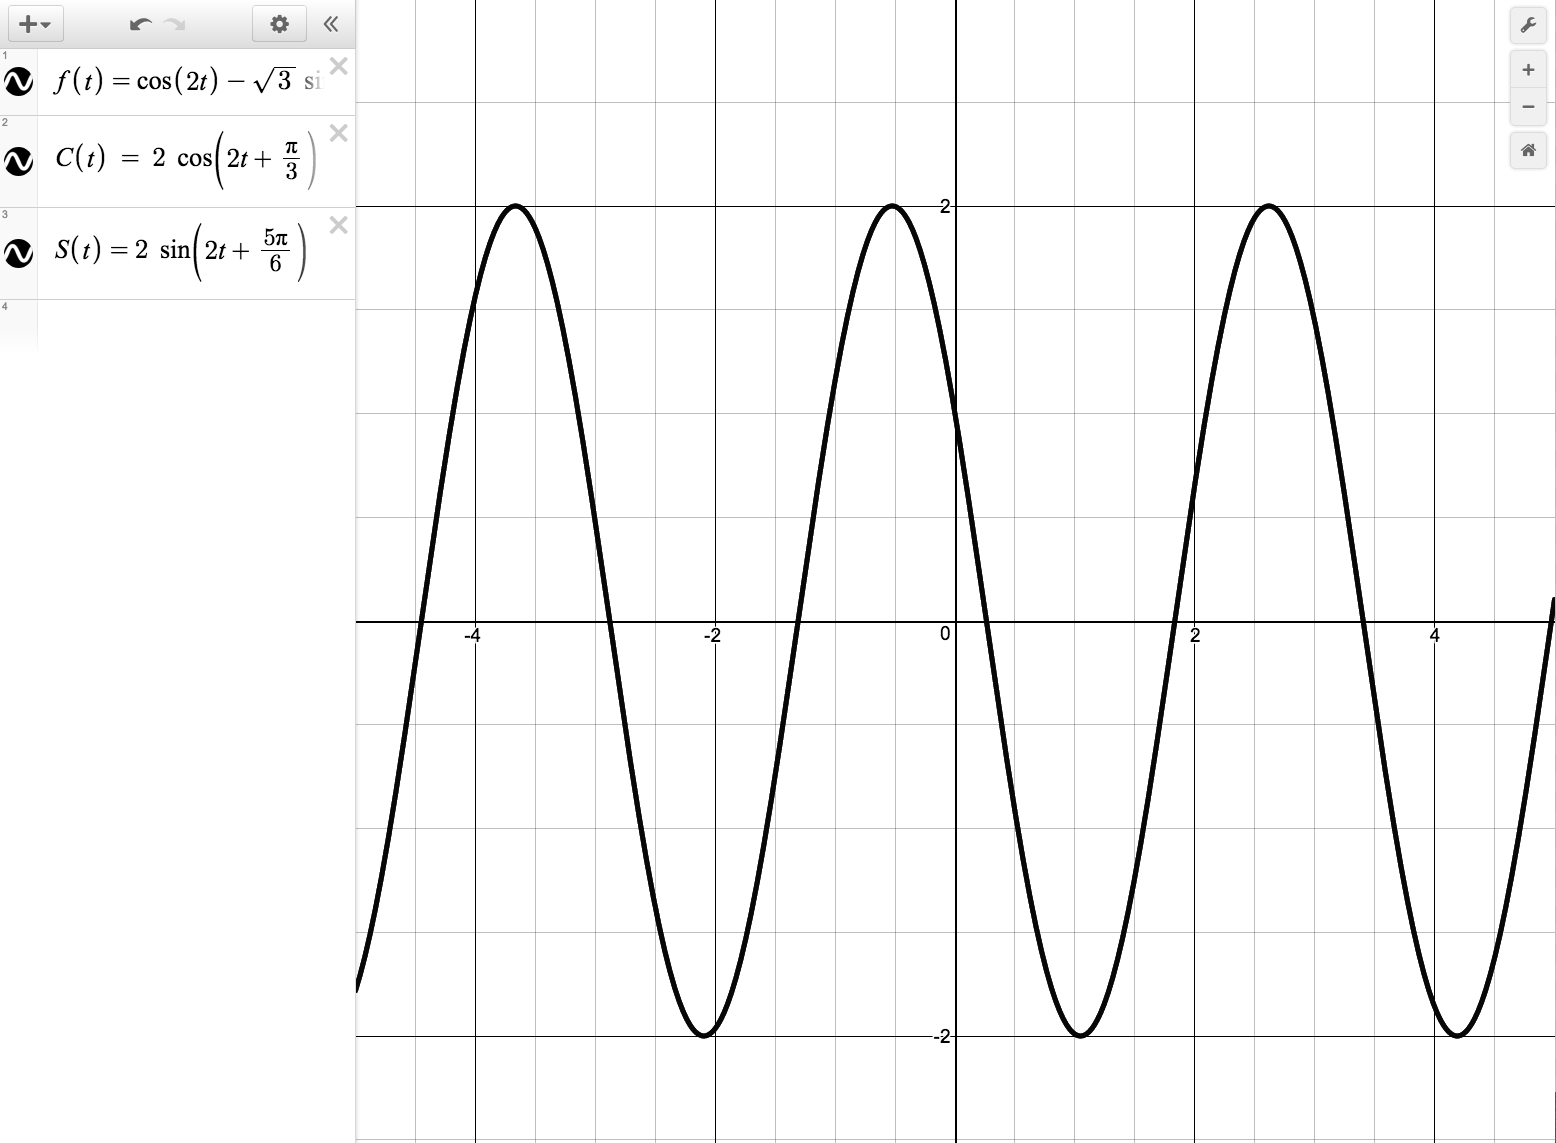
\includegraphics[width=4in]{./MoreTrigonometricIdentitiesGraphics/ExpandedSinusoidExample.jpg} 



\end{center}

\qed

\end{enumerate}

\end{ex}

A couple of remarks about Example \ref{expandedsinusoidex1} are in order.   First, had we chosen  $A = -2$ instead of $A = 2$ as we worked through Example \ref{expandedsinusoidex1}, our final answers would have \textit{looked} different. The reader is encouraged to rework Example  \ref{expandedsinusoidex1} using $A = -2$ to see what these differences are, and then for a challenging exercise, use identities to show that the formulas are all equivalent.\footnote{The general equations to fit a function of the form $f(x) = a \, \cos(\omega x) + b \, \sin(\omega x) + B$ into one of the forms in Theorem \ref{sinusoidform} are explored in Exercise \ref{sinusoidexercise1}.}

\smallskip

It is important to note that in order for the technique presented in Example \ref{expandedsinusoidex1} to fit a function into one of the forms in Theorem \ref{sinusoidform},  the \textit{frequencies} of the sine and cosine terms much match.  For example,  in the Exercises, you'll be asked to write $f(t) = 3\sqrt{3}\sin(3t) - 3\cos(3t)$ in the form of $S(t)$ and $C(t)$ above, and since both the sine and cosine terms have frequency $3$, this is possible.

\smallskip

However, a function such as  $f(t) = \sin(t) - \sin(3t)$ cannot be written in the form of $S(t)$ or $C(t)$. The quickest way to see this is to examine its graph below which is decidedly not a sinusoid.  That being said, we can still analyze this curve using identities.

\phantomsection
\label{beats}

\smallskip


\begin{center}

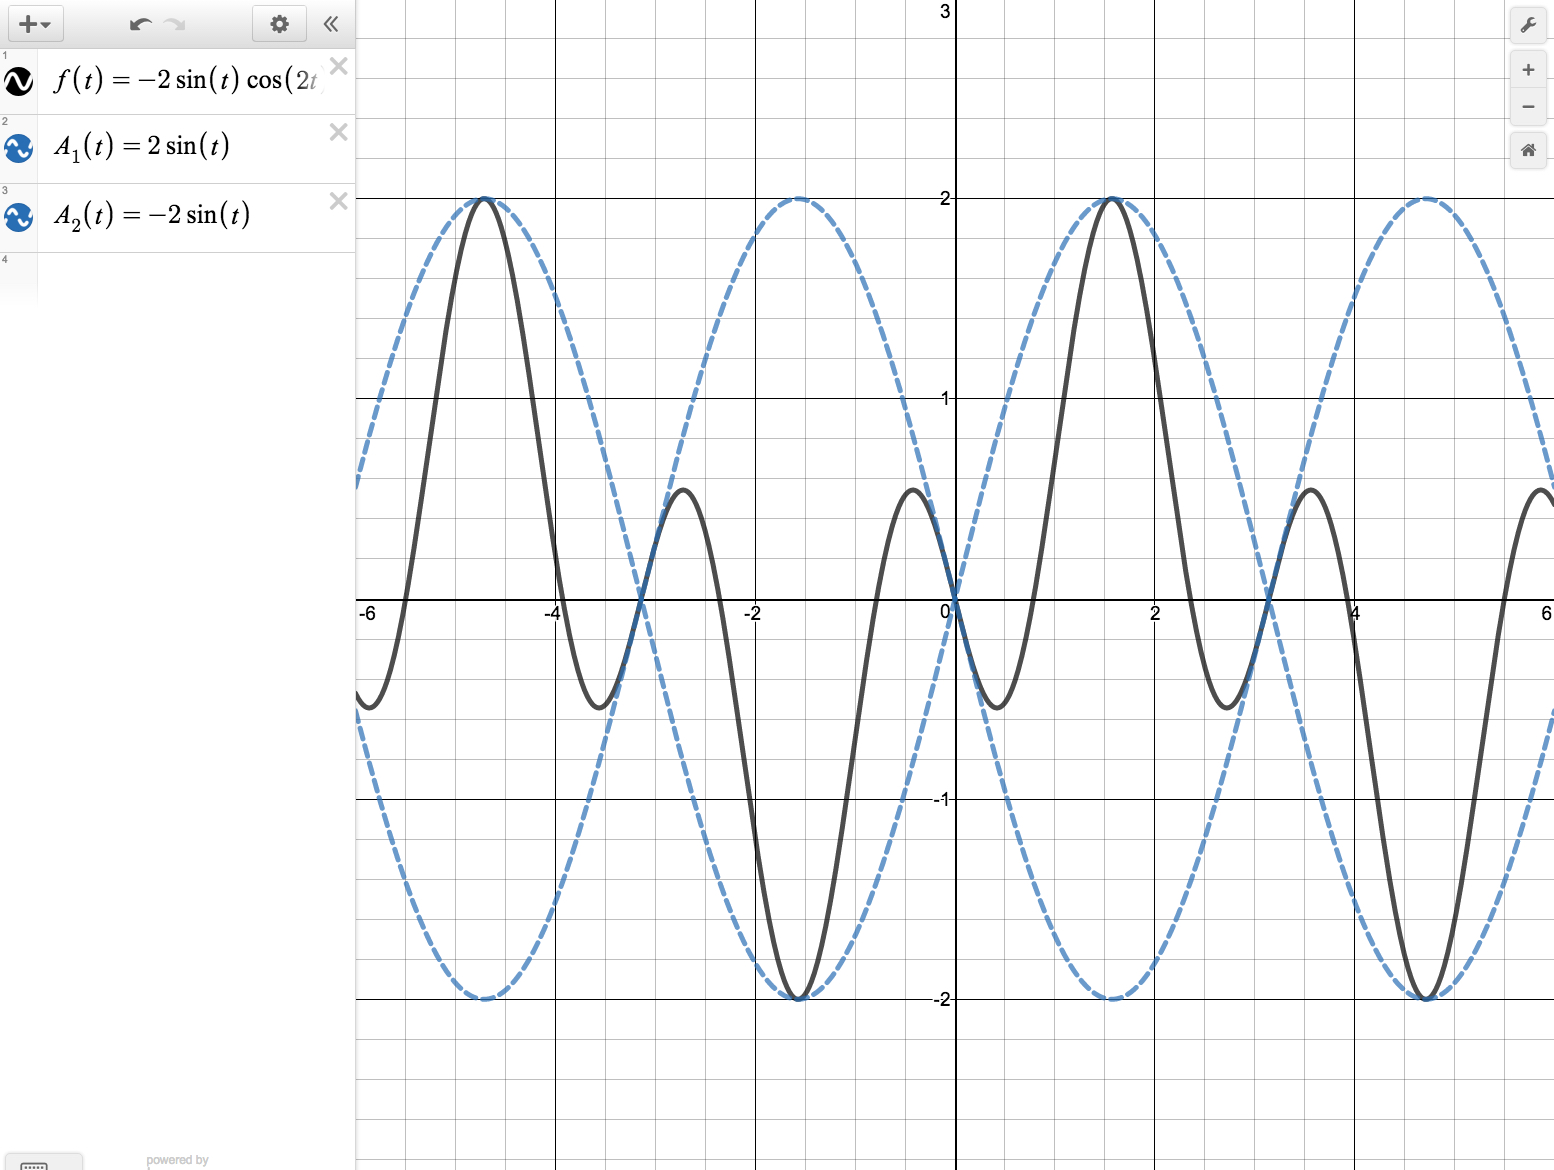
\includegraphics[width=4in]{./MoreTrigonometricIdentitiesGraphics/Beats.jpg} 

\end{center}


 Using our result from  number \ref{beatsprodsumex} Example \ref{prodtosumtoprod}, we may rewrite $f(t) = \sin(t) - \sin(3t) = -2 \sin(t) \cos(2t)$.  Grouping factors, we can view $f(t) = [ -2 \sin(t) ] \cos(2t) = A(t) \cos(2t)$ as the curve $y = \cos(2t)$ with a \textit{variable} amplitude, $A(t) = -2 \sin(t)$. 
 
 \smallskip
 
 Overlaying the graphs of $f(t)$ with the (dashed) graphs of $A_{1}(t) = 2 \sin(t)$ and $A_{2}(t) = -2 \sin(t)$, we can see the role these two curves play in the graph of $y = f(t)$.  They create a kind of `wave envelope' for the graph of $y = f(t)$.  This is an example of the \href{https://en.wikipedia.org/wiki/Beat_(acoustics)}{\underline{beats}} phenomenon.  Note that when written as a product of sinusoids, it is always the \textit{lower} frequency factor which creates the `wave-envelope' of the curve.
 
 \smallskip
 
Note that  in order to rewrite a sum or difference of sine and cosine functions with different frequencies into a product  using the sum to product identities, Theorem \ref{sumtoproduct}, we need the \textit{amplitudes} of each term to be the same.  We explore more examples of these functions and this behavior in the Exercises.
  

\smallskip


\newpage

\subsection{Exercises}

In Exercises \ref{evenoddfirst} - \ref{evenoddlast}, use the Even / Odd Identities to verify the identity.  Assume all quantities are defined.

\begin{multicols}{2}

\begin{enumerate}

\item $\sin(3\pi - 2\theta) = -\sin(2\theta - 3\pi)$ \vphantom{$\left( -\frac{\pi}{4} \right)$} \label{evenoddfirst}
\item $\cos \left( -\frac{\pi}{4} - 5t \right) = \cos \left( 5t + \frac{\pi}{4} \right)$

\setcounter{HW}{\value{enumi}}

\end{enumerate}

\end{multicols}

\begin{multicols}{2}

\begin{enumerate}

\setcounter{enumi}{\value{HW}}

\item $\tan(-x^{2} + 1) = -\tan(x^{2} - 1)$
\item $\csc(-\theta - 5) = -\csc(\theta + 5)$

\setcounter{HW}{\value{enumi}}

\end{enumerate}

\end{multicols}

\begin{multicols}{2}

\begin{enumerate}

\setcounter{enumi}{\value{HW}}

\item $\sec(-6x) = \sec(6x)$
\item $\cot(9 - 7\theta) = -\cot(7\theta - 9)$ \label{evenoddlast}

\setcounter{HW}{\value{enumi}}

\end{enumerate}

\end{multicols}

In Exercises \ref{sumdifffirst} - \ref{sumdifflast}, use the Sum and Difference Identities to find the exact value.  You may have need of the Quotient, Reciprocal or Even / Odd Identities as well.

\begin{multicols}{3}

\begin{enumerate}

\setcounter{enumi}{\value{HW}}

\item  \label{cos75} $\cos(75^{\circ})$ \label{sumdifffirst} 
\item  $\sec(165^{\circ})$
\item  \label{sin105} $\sin(105^{\circ})$

\setcounter{HW}{\value{enumi}}

\end{enumerate}

\end{multicols}

\begin{multicols}{3}

\begin{enumerate}

\setcounter{enumi}{\value{HW}}

\item  $\csc(195^{\circ})$
\item  $\cot(255^{\circ})$
\item  $\tan(375^{\circ})$

\setcounter{HW}{\value{enumi}}

\end{enumerate}

\end{multicols}

\begin{multicols}{3}

\begin{enumerate}

\setcounter{enumi}{\value{HW}}

\item  $\cos\left(\frac{13\pi}{12}\right)$
\item  $\sin\left(\frac{11\pi}{12}\right)$
\item  $\tan\left(\frac{13\pi}{12}\right)$

\setcounter{HW}{\value{enumi}}

\end{enumerate}

\end{multicols}

\begin{multicols}{3}

\begin{enumerate}

\setcounter{enumi}{\value{HW}}

\item \label{cos7pi12} $\cos \left( \frac{7\pi}{12} \right)$
\item $\tan \left( \frac{17\pi}{12} \right)$
\item \label{sinpi12} $\sin \left( \frac{\pi}{12} \right)$ \vphantom{$\left(\frac{13\pi}{12}\right)$}

\setcounter{HW}{\value{enumi}}

\end{enumerate}

\end{multicols}

\begin{multicols}{3}

\begin{enumerate}

\setcounter{enumi}{\value{HW}}

\item $\cot \left( \frac{11\pi}{12} \right)$
\item $\csc \left( \frac{5\pi}{12} \right)$
\item $\sec \left( -\frac{\pi}{12} \right)$ \vphantom{$\left(\frac{13\pi}{12}\right)$} \label{sumdifflast}

\setcounter{HW}{\value{enumi}}

\end{enumerate}

\end{multicols}

\begin{enumerate}

\setcounter{enumi}{\value{HW}}

\item  If $\alpha$ is a Quadrant IV angle with $\cos(\alpha) = \frac{\sqrt{5}}{5}$, and  $\sin(\beta) = \frac{\sqrt{10}}{10}$, where $\frac{\pi}{2} < \beta < \pi$, find

\begin{multicols}{3}

\begin{enumerate}

\item  $\cos(\alpha + \beta)$
\item  $\sin(\alpha + \beta)$
\item  $\tan(\alpha + \beta)$

\setcounter{HWindent}{\value{enumii}}

\end{enumerate}

\end{multicols}

\begin{multicols}{3}

\begin{enumerate}

\setcounter{enumii}{\value{HWindent}}

\item  $\cos(\alpha - \beta)$
\item  $\sin(\alpha - \beta)$
\item  $\tan(\alpha - \beta)$

\end{enumerate}

\end{multicols}

\item  If $\csc(\alpha) = 3$, where $0 < \alpha < \frac{\pi}{2}$, and $\beta$ is a Quadrant II angle with $\tan(\beta) = -7$, find

\begin{multicols}{3}

\begin{enumerate}

\item  $\cos(\alpha + \beta)$
\item  $\sin(\alpha + \beta)$
\item  $\tan(\alpha + \beta)$

\setcounter{HWindent}{\value{enumii}}

\end{enumerate}

\end{multicols}

\begin{multicols}{3}

\begin{enumerate}

\setcounter{enumii}{\value{HWindent}}

\item  $\cos(\alpha - \beta)$
\item  $\sin(\alpha - \beta)$
\item  $\tan(\alpha - \beta)$

\end{enumerate}

\end{multicols}

\item If $\sin(\alpha) = \frac{3}{5}$, where $0 < \alpha < \frac{\pi}{2}$, and $\cos(\beta) = \frac{12}{13}$ where $\frac{3\pi}{2} < \beta < 2\pi$, find 

\begin{multicols}{3}

\begin{enumerate}

\item $\sin(\alpha + \beta)$
\item $\cos(\alpha - \beta)$
\item $\tan(\alpha - \beta)$

\end{enumerate}

\end{multicols}



\item If $\sec(\alpha) = -\frac{5}{3}$, where $\frac{\pi}{2} < \alpha < \pi$, and $\tan(\beta) = \frac{24}{7}$, where $\pi < \beta < \frac{3\pi}{2}$, find

\begin{multicols}{3}

\begin{enumerate}

\item $\csc(\alpha - \beta)$
\item $\sec(\alpha + \beta)$
\item $\cot(\alpha + \beta)$

\end{enumerate}

\end{multicols}

\setcounter{HW}{\value{enumi}}

\end{enumerate}

\newpage

In Exercises \ref{expandedsinusoidexerfirst} - \ref{expandedsinusoidexerlast}, use Example \ref{expandedsinusoidex1} as a guide to show that the function is a sinusoid by rewriting it in the forms $C(t) = A \cos(\omega t + \phi) + B$ and $S(t) = A \sin(\omega t + \phi) + B$ for $\omega > 0$ and $0 \leq \phi < 2\pi$.

\begin{multicols}{2}

\begin{enumerate}

\setcounter{enumi}{\value{HW}}

\item $f(t) = \sqrt{2}\sin(t) + \sqrt{2}\cos(t) + 1$ \label{expandedsinusoidexerfirst}
\item $f(t) = 3\sqrt{3}\sin(3t) - 3\cos(3t)$

\setcounter{HW}{\value{enumi}}

\end{enumerate}

\end{multicols}

\begin{multicols}{2}

\begin{enumerate}

\setcounter{enumi}{\value{HW}}

\item $f(t) = -\sin(t) + \cos(t) - 2$ \vphantom{$\left( -\frac{1\sqrt{3}}{2} \right)$} 
\item $f(t) = -\frac{1}{2}\sin(2t) - \frac{\sqrt{3}}{2}\cos(2t)$

\setcounter{HW}{\value{enumi}}

\end{enumerate}

\end{multicols}

\begin{multicols}{2}

\begin{enumerate}

\setcounter{enumi}{\value{HW}}

\item  $f(t) = 2\sqrt{3} \cos(t) - 2\sin(t)$ \vphantom{$\left( -\frac{3\sqrt{3}}{2} \right)$} 
\item  $f(t) = \frac{3}{2} \cos(2t) - \frac{3\sqrt{3}}{2} \sin(2t) + 6$

\setcounter{HW}{\value{enumi}}

\end{enumerate}

\end{multicols}

\begin{multicols}{2}

\begin{enumerate}

\setcounter{enumi}{\value{HW}}

\item  $f(t) = -\frac{1}{2} \cos(5t) -\frac{\sqrt{3}}{2} \sin(5t)$
\item  $f(t) = -6\sqrt{3} \cos(3t) - 6\sin(3t) - 3$ \vphantom{$\left( -\frac{\sqrt{3}}{2} \right)$} 

\setcounter{HW}{\value{enumi}}

\end{enumerate}

\end{multicols}

\begin{multicols}{2}

\begin{enumerate}

\setcounter{enumi}{\value{HW}}

\item  $f(t) =  \frac{5\sqrt{2}}{2} \sin(t)  -\frac{5\sqrt{2}}{2} \cos(t)$
\item  $f(t) =3 \sin \left(\frac{t}{6}\right) -3\sqrt{3} \cos \left(\frac{t}{6}\right)$ \vphantom{$\left( \frac{-5 \sqrt{3}}{2} \right)$}  \label{expandedsinusoidexerlast}

\setcounter{HW}{\value{enumi}}

\end{enumerate}

\end{multicols}


\begin{enumerate}

\setcounter{enumi}{\value{HW}}

\item In Exercises \ref{expandedsinusoidexerfirst} - \ref{expandedsinusoidexerlast}, you should have noticed a relationship between the phases $\phi$ for the $S(t)$ and $C(t)$.  Show that if $f(t) = A \sin(\omega t + \alpha) + B$, then $f(t) = A \cos(\omega t + \beta) + B$ where $\beta = \alpha - \frac{\pi}{2}$. 
\label{sinusoidexercise1}

\item Let $\phi$ be an angle measured in radians and let $P(a,b)$ be a point on the terminal side of $\phi$ when it is drawn in standard position.  Use Theorem \ref{cosinesinecircle} and the sum identity for sine in Theorem \ref{sinesumdifference} to show that  $f(t) = a \, \sin(\omega t) + b\, \cos(\omega t) + B$ (with  $\omega > 0$) can be rewritten as $f(t) = \sqrt{a^{2} + b^{2}}\sin(\omega t + \phi) + B$.
\label{sinusoidexercise2}

\setcounter{HW}{\value{enumi}}

\end{enumerate}

\begin{enumerate}

\setcounter{enumi}{\value{HW}}

\item  \label{twodaylightfunctions} In Example \ref{sinusoidsunlight} in Section \ref{GraphsofSineandCosine}, we developed two (seemingly) different formulas to model the hours of daylight, $H(t)$:   $H_{1}(t) = 9.25 \sin\left(\frac{\pi}{6} t - \frac{\pi}{2}\right) + 12.55$ and  $H_{2}(t) = -8.13 \sin\left(\frac{\pi}{6} t - 4.70\right)+ 12.5$.  Use the difference identities for sine to expand $H_{1}(t)$ and $H_{2}(t)$.  How different are they?
\setcounter{HW}{\value{enumi}}
\end{enumerate}




In Exercises \ref{identfirstident} - \ref{identlastident}, verify the identity.\footnote{Note: numbers \ref{conversionsineshift} and \ref{conversioncosineshift} are the conversion formulas stated in Theorem \ref{cosinesinefunctionprops} in Section \ref{GraphsofSineandCosine}.}

\begin{multicols}{2}

\begin{enumerate}

\setcounter{enumi}{\value{HW}}

\item  $\sin\left(\theta + \frac{\pi}{2}\right) = \cos(t)$  \label{identfirstident} \label{conversionsineshift}
\item $\cos\left(\theta - \frac{\pi}{2} \right) = \sin(t)$ \label{conversioncosineshift}

\setcounter{HW}{\value{enumi}}

\end{enumerate}

\end{multicols}


\begin{multicols}{2}

\begin{enumerate}

\setcounter{enumi}{\value{HW}}

\item $\cos(\theta - \pi) = -\cos(\theta)$
\item $\sin(\pi - \theta) = \sin(\theta)$

\setcounter{HW}{\value{enumi}}

\end{enumerate}

\end{multicols}

\begin{multicols}{2}

\begin{enumerate}

\setcounter{enumi}{\value{HW}}

\item $\tan\left(\theta + \frac{\pi}{2} \right) = -\cot(\theta)$
\item $\sin(\alpha + \beta) + \sin(\alpha - \beta) = 2\sin(\alpha)\cos(\beta)$ \vphantom{$\left( \frac{\pi}{2} \right)$}

\setcounter{HW}{\value{enumi}}

\end{enumerate}

\end{multicols}

\begin{multicols}{2}

\begin{enumerate}

\setcounter{enumi}{\value{HW}}

\item $\sin(\alpha + \beta) - \sin(\alpha - \beta) = 2\cos(\alpha) \sin(\beta)$
\item $\cos(\alpha + \beta) + \cos(\alpha - \beta) = 2\cos(\alpha) \cos(\beta)$

\setcounter{HW}{\value{enumi}}

\end{enumerate}

\end{multicols}

\begin{multicols}{2}

\begin{enumerate}

\setcounter{enumi}{\value{HW}}

\item $\cos(\alpha + \beta) - \cos(\alpha - \beta) = -2\sin(\alpha) \sin(\beta)$ \vphantom{$\dfrac{\sin(\alpha+\beta)}{\sin(\alpha-\beta)}$}
\item $\dfrac{\sin(\alpha+\beta)}{\sin(\alpha-\beta)} = \dfrac{1+\cot(\alpha) \tan(\beta)}{1 - \cot(\alpha) \tan(\beta)}$ 

\setcounter{HW}{\value{enumi}}

\end{enumerate}

\end{multicols}

\begin{multicols}{2}

\begin{enumerate}

\setcounter{enumi}{\value{HW}}

\item $\dfrac{\cos(\alpha + \beta)}{\cos(\alpha - \beta)} = \dfrac{1 - \tan(\alpha)\tan(\beta)}{1 + \tan(\alpha)\tan(\beta)}$
\item $\dfrac{\tan(\alpha + \beta)}{\tan(\alpha - \beta)} = \dfrac{\sin(\alpha)\cos(\alpha) + \sin(\beta)\cos(\beta)}{\sin(\alpha)\cos(\alpha) - \sin(\beta)\cos(\beta)}$

\setcounter{HW}{\value{enumi}}

\end{enumerate}

\end{multicols}

\begin{enumerate}

\setcounter{enumi}{\value{HW}}

\item $\dfrac{\sin(t + h) - \sin(t)}{h} = \cos(t) \left(\dfrac{\sin(h)}{h} \right) + \sin(t) \left( \dfrac{\cos(h) - 1}{h} \right)$
\item $\dfrac{\cos(t + h) - \cos(t)}{h} = \cos(t) \left( \dfrac{\cos(h) - 1}{h} \right) - \sin(t) \left(\dfrac{\sin(h)}{h} \right)$
\item  $\dfrac{\tan(t + h) - \tan(t)}{h} = \left( \dfrac{\tan(h)}{h} \right) \left(\dfrac{\sec^{2}(t)}{1 - \tan(t)\tan(h)} \right)$ \label{identlastident}

\setcounter{HW}{\value{enumi}}

\end{enumerate}



In Exercises \ref{idenhalfanglefirst} - \ref{idenhalfanglelast}, use the Half Angle Formulas to find the exact value.  You may have need of the Quotient, Reciprocal or Even / Odd Identities as well.

\begin{multicols}{2}

\begin{enumerate}

\setcounter{enumi}{\value{HW}}

\item  $\cos(75^{\circ})$  (compare with Exercise \ref{cos75}) \label{idenhalfanglefirst}
\item  $\sin(105^{\circ})$  (compare with Exercise \ref{sin105})

\setcounter{HW}{\value{enumi}}

\end{enumerate}

\end{multicols}

\begin{multicols}{2}

\begin{enumerate}

\setcounter{enumi}{\value{HW}}

\item  $\cos(67.5^{\circ})$
\item  $\sin(157.5^{\circ})$

\setcounter{HW}{\value{enumi}}

\end{enumerate}

\end{multicols}

\begin{multicols}{2}

\begin{enumerate}

\setcounter{enumi}{\value{HW}}

\item  $\tan(112.5^{\circ})$ \vphantom{$\left( \frac{7\pi}{12} \right)$}
\item  $\cos\left( \frac{7\pi}{12} \right)$  (compare with Exercise \ref{cos7pi12})

\setcounter{HW}{\value{enumi}}

\end{enumerate}

\end{multicols}

\begin{multicols}{2}

\begin{enumerate}

\setcounter{enumi}{\value{HW}}

\item  $\sin\left( \frac{\pi}{12} \right)$  (compare with Exercise \ref{sinpi12})
\item $\cos \left( \frac{\pi}{8} \right)$

\setcounter{HW}{\value{enumi}}

\end{enumerate}

\end{multicols}

\begin{multicols}{2}

\begin{enumerate}

\setcounter{enumi}{\value{HW}}

\item $\sin \left( \frac{5\pi}{8} \right)$
\item $\tan \left( \frac{7\pi}{8} \right)$ \label{idenhalfanglelast}

\setcounter{HW}{\value{enumi}}

\end{enumerate}

\end{multicols}

In Exercises \ref{doublehalffirst} - \ref{doublehalflast}, use the given information about $\theta$ to find the exact values of 

\begin{multicols}{3}

\begin{itemize}

\item $\sin(2\theta)$
\item $\sin\left(\frac{\theta}{2}\right)$
\item $\cos(2\theta)$
\item $\cos\left(\frac{\theta}{2}\right)$
\item $\tan(2\theta)$
\item $\tan\left(\frac{\theta}{2}\right)$

\end{itemize}

\end{multicols}

\begin{multicols}{2}

\begin{enumerate}

\setcounter{enumi}{\value{HW}}

\item $\sin(\theta) = -\frac{7}{25}$ where $\frac{3\pi}{2} < \theta < 2\pi$ \label{doublehalffirst}
\item $\cos(\theta) = \frac{28}{53}$ where $0 < \theta < \frac{\pi}{2}$

\setcounter{HW}{\value{enumi}}

\end{enumerate}

\end{multicols}

\begin{multicols}{2}

\begin{enumerate}

\setcounter{enumi}{\value{HW}}

\item $\tan(\theta) = \frac{12}{5}$ where $\pi < \theta < \frac{3\pi}{2}$
\item $\csc(\theta) = 4$ where $\frac{\pi}{2} < \theta < \pi$

\setcounter{HW}{\value{enumi}}

\end{enumerate}

\end{multicols}

\begin{multicols}{2}

\begin{enumerate}

\setcounter{enumi}{\value{HW}}

\item  $\cos(\theta) = \frac{3}{5}$ where $0 < \theta < \frac{\pi}{2}$
\item  $\sin(\theta) = -\frac{4}{5}$ where $\pi < \theta < \frac{3\pi}{2}$

\setcounter{HW}{\value{enumi}}

\end{enumerate}

\end{multicols}

\begin{multicols}{2}

\begin{enumerate}

\setcounter{enumi}{\value{HW}}

\item  $\cos(\theta) = \frac{12}{13}$ where $\frac{3\pi}{2} < \theta < 2\pi$
\item  $\sin(\theta) = \frac{5}{13}$ where $\frac{\pi}{2} < \theta < \pi$

\setcounter{HW}{\value{enumi}}

\end{enumerate}

\end{multicols}

\begin{multicols}{2}

\begin{enumerate}

\setcounter{enumi}{\value{HW}}

\item  $\sec(\theta) = \sqrt{5}$ where $\frac{3\pi}{2} < \theta < 2\pi$
\item  $\tan(\theta) = -2$ where $\frac{\pi}{2} < \theta < \pi$ \label{doublehalflast}

\setcounter{HW}{\value{enumi}}

\end{enumerate}

\end{multicols}



In Exercises \ref{moreidentfirst} - \ref{moreidentlast}, verify the identity.  Assume all quantities are defined.

\begin{multicols}{2}

\begin{enumerate}

\setcounter{enumi}{\value{HW}}

\item  $(\cos(\theta) + \sin(\theta))^2 = 1 + \sin(2\theta)$ \label{moreidentfirst}
\item  $(\cos(\theta) - \sin(\theta))^2 = 1 - \sin(2\theta)$

\setcounter{HW}{\value{enumi}}

\end{enumerate}

\end{multicols}

\begin{multicols}{2}

\begin{enumerate}

\setcounter{enumi}{\value{HW}}

\item  $\tan(2t) = \frac{1}{1-\tan(t)} - \frac{1}{1+\tan(t)}$
\item  $\csc(2\theta) = \frac{\cot(\theta) + \tan(\theta)}{2}$

\setcounter{HW}{\value{enumi}}

\end{enumerate}

\end{multicols}

\begin{multicols}{2}

\begin{enumerate}

\setcounter{enumi}{\value{HW}}

\item  $8 \sin^{4}(x) = \cos(4x) - 4\cos(2x)+3$
\item  $8 \cos^{4}(x) = \cos(4x) + 4\cos(2x)+3$

\setcounter{HW}{\value{enumi}}

\end{enumerate}

\end{multicols}

\begin{multicols}{2}

\begin{enumerate}

\setcounter{enumi}{\value{HW}}

\item \label{sine3theta} $\sin(3\theta) = 3\sin(\theta) - 4\sin^{3}(\theta)$
\item  $\sin(4\theta) = 4\sin(\theta)\cos^{3}(\theta) - 4\sin^{3}(\theta)\cos(\theta)$

\setcounter{HW}{\value{enumi}}

\end{enumerate}

\end{multicols}

\begin{enumerate}

\setcounter{enumi}{\value{HW}}

\item  $32\sin^{2}(t) \cos^{4}(t) = 2 + \cos(2t) - 2\cos(4t) - \cos(6t)$
\item  $32\sin^{4}(t) \cos^{2}(t) = 2 - \cos(2t) - 2\cos(4t) + \cos(6t)$
\item \label{cosine4theta} $\cos(4\theta) = 8\cos^{4}(\theta) - 8\cos^{2}(\theta) + 1$
\item  $\cos(8\theta) = 128\cos^{8}(\theta)-256\cos^{6}(\theta)+160\cos^{4}(\theta)-32\cos^{2}(\theta)+1$ (HINT:  Use the result to \ref{cosine4theta}.)
\item  $\sec(2x) = \dfrac{\cos(x)}{\cos(x) + \sin(x)} + \dfrac{\sin(x)}{\cos(x)-\sin(x)}$ 
\item  $\dfrac{1}{\cos(\theta) - \sin(\theta)} + \dfrac{1}{\cos(\theta) + \sin(\theta)} = \dfrac{2\cos(\theta)}{\cos(2\theta)}$
\item  $\dfrac{1}{\cos(\theta) - \sin(\theta)} - \dfrac{1}{\cos(\theta) + \sin(\theta)} = \dfrac{2\sin(\theta)}{\cos(2\theta)}$ \label{moreidentlast}

\setcounter{HW}{\value{enumi}}

\end{enumerate}

\begin{enumerate}

\setcounter{enumi}{\value{HW}}

\item  \label{preludetoarctrigsine} Suppose $\theta$ is a Quadrant I angle with $\sin(\theta) = x$. Verify the following formulas

\begin{multicols}{3}

\begin{enumerate}

\item  $\cos(\theta) = \sqrt{1-x^2}$

\item  $\sin(2\theta) = 2x\sqrt{1-x^2}$

\item $\cos(2\theta) = 1 - 2x^2$

\end{enumerate}

\end{multicols}

\item  Discuss with your classmates how each of the formulas, if any, in Exercise \ref{preludetoarctrigsine} change if we change assume $\theta$ is a Quadrant II, III, or IV angle.

\item  \label{preludetoarctrigtan} Suppose $\theta$ is a Quadrant I angle with $\tan(\theta) = x$. Verify the following formulas

\begin{multicols}{2}

\begin{enumerate}

\item $\cos(\theta) = \dfrac{1}{\sqrt{x^2+1}}$
\item $\sin(\theta) = \dfrac{x}{\sqrt{x^2+1}}$

\setcounter{HWindent}{\value{enumii}}

\end{enumerate}

\end{multicols}

\begin{multicols}{2}

\begin{enumerate}

\setcounter{enumii}{\value{HWindent}}

\item $\sin(2\theta) = \dfrac{2x}{x^2+1}$
\item $\cos(2\theta) = \dfrac{1-x^2}{x^2+1}$

\end{enumerate}

\end{multicols}

\item  Discuss with your classmates how each of the formulas, if any, in Exercise \ref{preludetoarctrigtan} change if we change assume $\theta$ is a Quadrant II, III, or IV angle.

\item  If $\sin(t) = x$ for  $-\frac{\pi}{2} < t < \frac{\pi}{2}$, find an expression for $\tan(t)$ in terms of $x$.

\item  If $\tan(\theta) = x$ for $-\frac{\pi}{2} < \theta < \frac{\pi}{2}$,  find an expression for $\sec(\theta)$ in terms of $x$.

\item  If $\sec(\theta) = x$ where  $\theta$ is a Quadrant II angle, find  an expression for $\tan(\theta)$ in terns of $x$.

\item If $\sin(t) = \frac{x}{2}$ for $-\frac{\pi}{2} < t < \frac{\pi}{2}$, find an expression for $\cos(2t)$ in terms of $x$.

\item If $\tan(\theta) = \frac{x}{7}$ for $-\frac{\pi}{2} < \theta < \frac{\pi}{2}$, find an expression for $\sin(2\theta)$ in terms of $x$.

\item If $\sec(t) = \frac{x}{4}$ for $0 < t < \frac{\pi}{2}$, find an expression for $\ln|\sec(t) + \tan(t)|$ in terms of $x$.

\item Show that $\cos^{2}(\theta) - \sin^{2}(\theta) = 2\cos^{2}(\theta) - 1 = 1 - 2\sin^{2}(\theta)$ for all $\theta$.

\item Let $\theta$ be a Quadrant III angle with $\cos(\theta) = -\frac{1}{5}$.  Show that this is not enough information to determine the sign of  $\sin\left(\frac{\theta}{2}\right)$ by first assuming $3\pi < \theta < \frac{7\pi}{2}$ and then assuming $\pi < \theta < \frac{3\pi}{2}$ and computing $\sin\left(\frac{\theta}{2}\right)$ in both cases.

\item Without using your calculator, show that $\frac{\sqrt{2 + \sqrt{3}}}{2} = \frac{\sqrt{6} + \sqrt{2}}{4}$

\item In part \ref{cosinepolynomial} of Example \ref{doubleangleex}, we wrote $\cos(3\theta)$ as a polynomial in terms of $\cos(\theta)$.  In Exercise \ref{cosine4theta}, we had you verify an identity which expresses $\cos(4\theta)$ as a polynomial in terms of $\cos(\theta)$.   Can you find a polynomial in terms of $\cos(\theta)$ for $\cos(5\theta)$?  $\cos(6\theta)$?  Can you find a pattern so that $\cos(n\theta)$ could be written as a polynomial in cosine for any natural number $n$?

\item In Exercise \ref{sine3theta}, we has you verify an identity which expresses $\sin(3\theta)$ as a polynomial in terms of $\sin(\theta)$.   Can you do the same for  $\sin(5\theta)$?  What about for $\sin(4\theta)$?  If not, what goes wrong?

\setcounter{HW}{\value{enumi}}

\end{enumerate}

In Exercises \ref{idengraphfirst} - \ref{idengraphlast}, verify the identity by graphing the right and left hand using a graphing utility.

\begin{multicols}{3}

\begin{enumerate}

\setcounter{enumi}{\value{HW}}

\item $\sin^{2}(t) + \cos^{2}(t) = 1$ \vphantom{$\left( \frac{\pi}{2} \right)$} \label{idengraphfirst} 
\item $\sec^{2}(x) - \tan^{2}(x) = 1$ \vphantom{$\left( \frac{\pi}{2} \right)$}
\item  $\cos(t) = \sin\left(\frac{\pi}{2} - t\right)$

\setcounter{HW}{\value{enumi}}

\end{enumerate}

\end{multicols}

\begin{multicols}{3}

\begin{enumerate}

\setcounter{enumi}{\value{HW}}

\item  $\tan(x+\pi) = \tan(x)$ \vphantom{$\frac{\sin(x)}{1+\cos(x)}$}
\item  $\sin(2t) = 2\sin(t)\cos(t)$ \vphantom{$\frac{\sin(x)}{1+\cos(x)}$}
\item  $\tan\left(\frac{x}{2}\right) = \frac{\sin(x)}{1+\cos(x)}$ \label{idengraphlast}

\setcounter{HW}{\value{enumi}}

\end{enumerate}

\end{multicols}


In Exercises \ref{prodsumfirst} - \ref{prodsumlast}, write the  given product as a sum. Note: you may need to use an Even/Odd Identity to match the answer provided.

\begin{multicols}{3}

\begin{enumerate}

\setcounter{enumi}{\value{HW}}

\item $\cos(3\theta)\cos(5\theta)$ \label{prodsumfirst}
\item $\sin(2t)\sin(7t)$
\item $\sin(9x)\cos(x)$

\setcounter{HW}{\value{enumi}}

\end{enumerate}

\end{multicols}

\begin{multicols}{3}

\begin{enumerate}

\setcounter{enumi}{\value{HW}}

\item $\cos(2\theta) \cos(6\theta)$
\item $\sin(3t) \sin(2t)$
\item $\cos(x) \sin(3x)$ \label{prodsumlast}

\setcounter{HW}{\value{enumi}}

\end{enumerate}

\end{multicols}

In Exercises \ref{sumprodfirst} - \ref{sumprodlast},  write the given sum as a product. Note:  you may need to use an Even/Odd or Cofunction Identity to match the answer provided.

\begin{multicols}{3}

\begin{enumerate}

\setcounter{enumi}{\value{HW}}

\item $\cos(3\theta) + \cos(5\theta)$ \label{sumprodfirst}
\item $\sin(2t) - \sin(7t)$
\item $\cos(5x) - \cos(6x)$

\setcounter{HW}{\value{enumi}}

\end{enumerate}

\end{multicols}

\begin{multicols}{3}

\begin{enumerate}

\setcounter{enumi}{\value{HW}}

\item $\sin(9\theta) - \sin(-\theta)$
\item $\sin(t) + \cos(t)$
\item $\cos(x) - \sin(x)$ \label{sumprodlast}

\setcounter{HW}{\value{enumi}}

\end{enumerate}

\end{multicols}


In Exercises \ref{beatexfirst} - \ref{beatexlast}, using the remarks following Example \ref{expandedsinusoidex1} on page \pageref{beats} as a guide,  rewrite the given function $f(t)$ as a product of sinusoids. Identify the functions which create the `wave envelope.' Check your answer by graphing  the function along with the `wave-envelope' using a graphing utility.

\begin{multicols}{2}

\begin{enumerate}

\setcounter{enumi}{\value{HW}}

\item $f(t) = \cos(3t) + \cos(5t)$ \label{beatexfirst}
\item $f(t) = 3\cos(5t) - 3\cos(6t)$
\setcounter{HW}{\value{enumi}}

\end{enumerate}

\end{multicols}

\begin{multicols}{2}

\begin{enumerate}

\setcounter{enumi}{\value{HW}}

\item $f(t) = \frac{1}{2} \sin(9t) + \frac{1}{2} \sin(t)$
\item $f(t) = \frac{2}{3}\sin(2t) - \frac{2}{3}\sin(7t)$\label{beatexlast}

\setcounter{HW}{\value{enumi}}

\end{enumerate}

\end{multicols}

\begin{enumerate}

\setcounter{enumi}{\value{HW}}

\item Verify the Even / Odd Identities for tangent, secant, cosecant and cotangent.

\item Verify the Cofunction Identities for tangent, secant, cosecant and cotangent.

\item Verify the Difference Identities for sine and tangent.

\item Verify the Product to Sum Identities.

\item Verify the Sum to Product Identities.

\end{enumerate}

\newpage

\subsection{Answers}

\begin{multicols}{2}

\begin{enumerate}

\addtocounter{enumi}{6}

\item  $\cos(75^{\circ}) = \frac{\sqrt{6} - \sqrt{2}}{4} $
\item  $\sec(165^{\circ}) = -\frac{4}{\sqrt{2}+\sqrt{6}} = \sqrt{2} - \sqrt{6}$

\setcounter{HW}{\value{enumi}}

\end{enumerate}

\end{multicols}

\begin{multicols}{2}

\begin{enumerate}

\setcounter{enumi}{\value{HW}}

\item  $\sin(105^{\circ}) = \frac{\sqrt{6}+\sqrt{2}}{4}$
\item  $\csc(195^{\circ}) = \frac{4}{\sqrt{2}-\sqrt{6}} = -(\sqrt{2}+\sqrt{6})$

\setcounter{HW}{\value{enumi}}

\end{enumerate}

\end{multicols}

\begin{multicols}{2}

\begin{enumerate}

\setcounter{enumi}{\value{HW}}

\item  $\cot(255^{\circ}) = \frac{\sqrt{3}-1}{\sqrt{3}+1} = 2-\sqrt{3}$
\item  $\tan(375^{\circ}) = \frac{3-\sqrt{3}}{3+\sqrt{3}} = 2-\sqrt{3}$

\setcounter{HW}{\value{enumi}}

\end{enumerate}

\end{multicols}

\begin{multicols}{2}

\begin{enumerate}

\setcounter{enumi}{\value{HW}}

\item  $\cos\left(\frac{13\pi}{12}\right) = -\frac{\sqrt{6}+\sqrt{2}}{4}$
\item  $\sin\left(\frac{11\pi}{12}\right) = \frac{\sqrt{6} - \sqrt{2}}{4}$

\setcounter{HW}{\value{enumi}}

\end{enumerate}

\end{multicols}

\begin{multicols}{2}

\begin{enumerate}

\setcounter{enumi}{\value{HW}}

\item  $\tan\left(\frac{13\pi}{12}\right) = \frac{3-\sqrt{3}}{3+\sqrt{3}} = 2-\sqrt{3}$
\item $\cos \left( \frac{7\pi}{12} \right) = \frac{\sqrt{2} - \sqrt{6}}{4}$

\setcounter{HW}{\value{enumi}}

\end{enumerate}

\end{multicols}

\begin{multicols}{2}

\begin{enumerate}

\setcounter{enumi}{\value{HW}}

\item $\tan \left( \frac{17\pi}{12} \right) = 2 + \sqrt{3}$
\item $\sin \left( \frac{\pi}{12} \right) = \frac{\sqrt{6} - \sqrt{2}}{4}$

\setcounter{HW}{\value{enumi}}

\end{enumerate}

\end{multicols}

\begin{multicols}{2}

\begin{enumerate}

\setcounter{enumi}{\value{HW}}

\item $\cot \left( \frac{11\pi}{12} \right) = -(2 + \sqrt{3})$
\item $\csc \left( \frac{5\pi}{12} \right) = \sqrt{6} - \sqrt{2}$

\setcounter{HW}{\value{enumi}}

\end{enumerate}

\end{multicols}

\begin{multicols}{2}

\begin{enumerate}

\setcounter{enumi}{\value{HW}}

\item $\sec \left( -\frac{\pi}{12} \right) = \sqrt{6} - \sqrt{2}$

\setcounter{HW}{\value{enumi}}

\end{enumerate}

\end{multicols}

\begin{enumerate}

\setcounter{enumi}{\value{HW}}

\item \begin{multicols}{2}

\begin{enumerate}

\item  $\cos(\alpha + \beta) = -\frac{\sqrt{2}}{10}$
\item  $\sin(\alpha + \beta) = \frac{7\sqrt{2}}{10}$

\setcounter{HWindent}{\value{enumii}}

\end{enumerate}

\end{multicols}

\begin{multicols}{2}

\begin{enumerate}

\setcounter{enumii}{\value{HWindent}}

\item  $\tan(\alpha + \beta) = -7$ \vphantom{$\frac{\sqrt{2}}{2}$}
\item  $\cos(\alpha - \beta)= -\frac{\sqrt{2}}{2}$

\setcounter{HWindent}{\value{enumii}}

\end{enumerate}

\end{multicols}

\begin{multicols}{2}

\begin{enumerate}

\setcounter{enumii}{\value{HWindent}}

\item  $\sin(\alpha - \beta) = \frac{\sqrt{2}}{2}$
\item  $\tan(\alpha - \beta) = -1$ \vphantom{$\frac{\sqrt{2}}{2}$}

\end{enumerate}

\end{multicols}

\item \begin{multicols}{2}

\begin{enumerate}

\item  $\cos(\alpha + \beta) = - \frac{4+7\sqrt{2}}{30}$
\item  $\sin(\alpha + \beta) = \frac{28-\sqrt{2}}{30}$

\setcounter{HWindent}{\value{enumii}}

\end{enumerate}

\end{multicols}

\begin{multicols}{2}

\begin{enumerate}

\setcounter{enumii}{\value{HWindent}}

\item  $\tan(\alpha + \beta) = \frac{-28+\sqrt{2}}{4+7\sqrt{2}} = \frac{63-100\sqrt{2}}{41}$
\item  $\cos(\alpha - \beta) =  \frac{-4+7\sqrt{2}}{30}$

\setcounter{HWindent}{\value{enumii}}

\end{enumerate}

\end{multicols}

\begin{multicols}{2}

\begin{enumerate}

\setcounter{enumii}{\value{HWindent}}

\item  $\sin(\alpha - \beta) = - \frac{28+\sqrt{2}}{30}$
\item  $\tan(\alpha - \beta)= \frac{28+\sqrt{2}}{4-7\sqrt{2}} = -\frac{63+100\sqrt{2}}{41}$

\end{enumerate}

\end{multicols}

\item \begin{multicols}{3}

\begin{enumerate}

\item $\sin(\alpha + \beta) = \frac{16}{65}$
\item $\cos(\alpha - \beta) = \frac{33}{65}$
\item $\tan(\alpha - \beta) = \frac{56}{33}$

\end{enumerate}

\end{multicols}

 

\item \begin{multicols}{3}

\begin{enumerate}

\item $\csc(\alpha - \beta) = -\frac{5}{4}$
\item $\sec(\alpha + \beta) = \frac{125}{117}$
\item $\cot(\alpha + \beta) = \frac{117}{44}$

\end{enumerate}

\end{multicols}

\setcounter{HW}{\value{enumi}}

\end{enumerate}

\begin{enumerate}
\setcounter{enumi}{\value{HW}}
\item $f(t) = \sqrt{2}\sin(t) + \sqrt{2}\cos(t) + 1 = 2\sin\left(t + \frac{\pi}{4}\right) + 1 = 2\cos\left(t + \frac{7\pi}{4}\right) + 1$ 
\item $f(t) = 3\sqrt{3}\sin(3t) - 3\cos(3t) = 6\sin\left(3t + \frac{11\pi}{6}\right) = 6\cos\left(3t + \frac{4\pi}{3}\right)$
\item $f(t) = -\sin(t) + \cos(t) - 2 = \sqrt{2}\sin\left(t + \frac{3\pi}{4}\right) - 2 = \sqrt{2}\cos\left(t + \frac{\pi}{4}\right) - 2$
\item $f(t) = -\frac{1}{2}\sin(2t) - \frac{\sqrt{3}}{2}\cos(2t) = \sin\left(2t + \frac{4\pi}{3}\right) = \cos\left(2t + \frac{5\pi}{6}\right)$
\item $f(t) = 2\sqrt{3} \cos(t) - 2\sin(t) = 4\sin\left(t+\frac{2\pi}{3}  \right)  = 4\cos\left(t + \frac{\pi}{6}\right)$
\item  $f(t) = \frac{3}{2} \cos(2t) - \frac{3\sqrt{3}}{2} \sin(2t) + 6 =3\sin\left(2t + \frac{5\pi}{6}\right) + 6   = 3\cos\left(2t + \frac{\pi}{3}\right) + 6$
\item  $f(t) = -\frac{1}{2} \cos(5t) -\frac{\sqrt{3}}{2} \sin(5t) =  \sin\left(5t + \frac{7\pi}{6}\right) = \cos\left(5t + \frac{2\pi}{3}\right)$
\item  $f(t) = -6\sqrt{3} \cos(3t) - 6\sin(3t) - 3 = 12\sin\left(3t + \frac{4\pi}{3}\right) - 3 = 12\cos\left(3t + \frac{5\pi}{6}\right) - 3$
\item  $f(t) =  \frac{5\sqrt{2}}{2} \sin(t)  -\frac{5\sqrt{2}}{2} \cos(t) = 5\sin\left(t + \frac{7\pi}{4}\right)= 5\cos\left(t + \frac{5\pi}{4}\right)$
\item  $f(t) =3\sin\left(\frac{t}{6}\right) -3\sqrt{3} \cos\left(\frac{t}{6}\right) = 6\sin\left( \frac{t}{6}+\frac{5\pi}{3}\right)= 6\cos\left( \frac{t}{6}+\frac{7\pi}{6}\right) $

\setcounter{HW}{\value{enumi}}
\end{enumerate}

\begin{multicols}{2}

\begin{enumerate}

\setcounter{enumi}{\value{HW}}

\addtocounter{enumi}{18}

\item $\cos(75^{\circ}) = \frac{\sqrt{2-\sqrt{3}}}{2}$ 
\item $\sin(105^{\circ}) = \frac{\sqrt{2+\sqrt{3}}}{2}$ 

\setcounter{HW}{\value{enumi}}

\end{enumerate}

\end{multicols}

\begin{multicols}{2}

\begin{enumerate}

\setcounter{enumi}{\value{HW}}

\item $\cos(67.5^{\circ})  = \frac{\sqrt{2-\sqrt{2}}}{2}$ 
\item $\sin(157.5^{\circ}) = \frac{\sqrt{2-\sqrt{2}}}{2}$ 

\setcounter{HW}{\value{enumi}}

\end{enumerate}

\end{multicols}

\begin{multicols}{2}

\begin{enumerate}

\setcounter{enumi}{\value{HW}}

\item $\tan(112.5^{\circ}) = - \sqrt{\frac{2+\sqrt{2}}{2-\sqrt{2}}} = -1 - \sqrt{2}$
\item $\cos\left( \frac{7\pi}{12} \right) = -\frac{\sqrt{2-\sqrt{3}}}{2}$  

\setcounter{HW}{\value{enumi}}

\end{enumerate}

\end{multicols}

\begin{multicols}{2}

\begin{enumerate}

\setcounter{enumi}{\value{HW}}

\item $\sin\left( \frac{\pi}{12} \right) = \frac{\sqrt{2-\sqrt{3}}}{2}$ 
\item $\cos \left( \frac{\pi}{8} \right) = \frac{\sqrt{2 + \sqrt{2}}}{2}$

\setcounter{HW}{\value{enumi}}

\end{enumerate}

\end{multicols}

\begin{multicols}{2}

\begin{enumerate}

\setcounter{enumi}{\value{HW}}

\item $\sin \left( \frac{5\pi}{8} \right) = \frac{\sqrt{2 + \sqrt{2}}}{2}$
\item $\tan \left( \frac{7\pi}{8} \right) = -\sqrt{ \frac{2 - \sqrt{2}}{2 + \sqrt{2}} } =1-\sqrt{2}$

\setcounter{HW}{\value{enumi}}

\end{enumerate}

\end{multicols}

\begin{enumerate}

\setcounter{enumi}{\value{HW}}

\item \begin{multicols}{3}

\begin{itemize}

\item $\sin(2\theta) = -\frac{336}{625}$
\item $\sin\left(\frac{\theta}{2}\right) = \frac{\sqrt{2}}{10}$
\item $\cos(2\theta) = \frac{527}{625}$
\item $\cos\left(\frac{\theta}{2}\right) = -\frac{7\sqrt{2}}{10}$
\item $\tan(2\theta) = -\frac{336}{527}$
\item $\tan\left(\frac{\theta}{2}\right) = -\frac{1}{7}$

\end{itemize}

\end{multicols}

\item \begin{multicols}{3}

\begin{itemize}

\item $\sin(2\theta) = \frac{2520}{2809}$
\item $\sin\left(\frac{\theta}{2}\right) = \frac{5\sqrt{106}}{106}$
\item $\cos(2\theta) = -\frac{1241}{2809}$
\item $\cos\left(\frac{\theta}{2}\right) = \frac{9\sqrt{106}}{106}$
\item $\tan(2\theta) = -\frac{2520}{1241}$
\item $\tan\left(\frac{\theta}{2}\right) = \frac{5}{9}$

\end{itemize}

\end{multicols}

\item \begin{multicols}{3}

\begin{itemize}

\item $\sin(2\theta) = \frac{120}{169}$
\item $\sin\left(\frac{\theta}{2}\right) = \frac{3\sqrt{13}}{13}$
\item $\cos(2\theta) = -\frac{119}{169}$
\item $\cos\left(\frac{\theta}{2}\right) = -\frac{2\sqrt{13}}{13}$
\item $\tan(2\theta) = -\frac{120}{119}$
\item $\tan\left(\frac{\theta}{2}\right) = -\frac{3}{2}$

\end{itemize}

\end{multicols}

\item \begin{multicols}{3}

\begin{itemize}

\item $\sin(2\theta) = -\frac{\sqrt{15}}{8}$
\item $\sin\left(\frac{\theta}{2}\right) =\frac{\sqrt{8+2\sqrt{15}}}{4} \\ \phantom{\tan\left(\frac{\theta}{2}\right) = 4+\sqrt{15}}$ 
\item $\cos(2\theta) = \frac{7}{8}$
\item $\cos\left(\frac{\theta}{2}\right) = \frac{\sqrt{8-2\sqrt{15}}}{4} \\ \phantom{\tan\left(\frac{\theta}{2}\right) = 4+\sqrt{15}} $
\item $\tan(2\theta) = -\frac{\sqrt{15}}{7}$
\item $\tan\left(\frac{\theta}{2}\right) = \sqrt{\frac{8+2\sqrt{15}}{8-2\sqrt{15}}} \\ \tan\left(\frac{\theta}{2}\right) = 4+\sqrt{15}$

\end{itemize}

\end{multicols}

\item \begin{multicols}{3}

\begin{itemize}

\item $\sin(2\theta) = \frac{24}{25}$
\item $\sin\left(\frac{\theta}{2}\right) = \frac{\sqrt{5}}{5}$
\item $\cos(2\theta) = -\frac{7}{25}$
\item $\cos\left(\frac{\theta}{2}\right) = \frac{2\sqrt{5}}{5}$
\item $\tan(2\theta)=-\frac{24}{7} $
\item $\tan\left(\frac{\theta}{2}\right) = \frac{1}{2}$

\end{itemize}

\end{multicols}



\item \begin{multicols}{3}

\begin{itemize}

\item $\sin(2\theta) = \frac{24}{25}$
\item $\sin\left(\frac{\theta}{2}\right) = \frac{2\sqrt{5}}{5}$
\item $\cos(2\theta) = -\frac{7}{25}$
\item $\cos\left(\frac{\theta}{2}\right) = -\frac{\sqrt{5}}{5}$
\item $\tan(2\theta)=-\frac{24}{7} $
\item $\tan\left(\frac{\theta}{2}\right) = -2$

\end{itemize}

\end{multicols}

\item \begin{multicols}{3}

\begin{itemize}

\item $\sin(2\theta) = -\frac{120}{169}$
\item $\sin\left(\frac{\theta}{2}\right) = \frac{\sqrt{26}}{26}$
\item $\cos(2\theta) = \frac{119}{169}$
\item $\cos\left(\frac{\theta}{2}\right) = -\frac{5\sqrt{26}}{26}$
\item $\tan(2\theta)=-\frac{120}{119}$
\item $\tan\left(\frac{\theta}{2}\right) = -\frac{1}{5}$

\end{itemize}

\end{multicols}

\item \begin{multicols}{3}

\begin{itemize}

\item $\sin(2\theta) = -\frac{120}{169}$
\item $\sin\left(\frac{\theta}{2}\right) = \frac{5\sqrt{26}}{26}$
\item $\cos(2\theta) = \frac{119}{169}$
\item $\cos\left(\frac{\theta}{2}\right) = \frac{\sqrt{26}}{26}$
\item $\tan(2\theta)=-\frac{120}{119}$
\item $\tan\left(\frac{\theta}{2}\right) = 5$

\end{itemize}

\end{multicols}

\item \begin{multicols}{3}

\begin{itemize}

\item $\sin(2\theta) = -\frac{4}{5}$
\item $\sin\left(\frac{\theta}{2}\right) = \frac{\sqrt{50-10\sqrt{5}}}{10} \\ \phantom{\tan\left(\frac{\theta}{2}\right) =\frac{5-5\sqrt{5}}{10}}$ 

\item $\cos(2\theta) = -\frac{3}{5}$
\item $\cos\left(\frac{\theta}{2}\right)= -\frac{\sqrt{50+10\sqrt{5}}}{10} \\ \phantom{\tan\left(\frac{\theta}{2}\right) =\frac{5-5\sqrt{5}}{10}}$ 
\item $\tan(2\theta)=\frac{4}{3}$
\item $\tan\left(\frac{\theta}{2}\right) =  -\sqrt{\frac{5-\sqrt{5}}{5+\sqrt{5}}} \\ \tan\left(\frac{\theta}{2}\right) =\frac{5-5\sqrt{5}}{10}$

\end{itemize}

\end{multicols}

\item \begin{multicols}{3}

\begin{itemize}

\item $\sin(2\theta) = -\frac{4}{5}$
\item $\sin\left(\frac{\theta}{2}\right) = \frac{\sqrt{50+10\sqrt{5}}}{10} \\ \phantom{\tan\left(\frac{\theta}{2}\right) =\frac{5-5\sqrt{5}}{10}}$ 

\item $\cos(2\theta) = -\frac{3}{5}$
\item $\cos\left(\frac{\theta}{2}\right)= \frac{\sqrt{50-10\sqrt{5}}}{10} \\ \phantom{\tan\left(\frac{\theta}{2}\right) =\frac{5-5\sqrt{5}}{10}}$ 
\item $\tan(2\theta)=\frac{4}{3}$
\item $\tan\left(\frac{\theta}{2}\right) =  \sqrt{\frac{5+\sqrt{5}}{5-\sqrt{5}}} \\ \tan\left(\frac{\theta}{2}\right) =\frac{5+5\sqrt{5}}{10}$

\end{itemize}

\end{multicols}

\setcounter{HW}{\value{enumi}}

\end{enumerate}

\begin{multicols}{3}
\begin{enumerate}
\setcounter{enumi}{\value{HW}}

\addtocounter{enumi}{19}

\item  $\tan(t) = \frac{x}{\sqrt{1 - x^2}}$

\item  $\sec(\theta) = \sqrt{1+x^2}$ \vphantom{$\tan(\theta) = \frac{x}{\sqrt{1 - x^2}}$}

\item  $\tan(\theta) = -\sqrt{x^2-1}$ \vphantom{$\tan(\theta) = \frac{x}{\sqrt{1 - x^2}}$}

\setcounter{HW}{\value{enumi}}
\end{enumerate}

\end{multicols}

\begin{multicols}{2}
\begin{enumerate}

\setcounter{enumi}{\value{HW}}

\item $\cos(2t) = 1 - \dfrac{x^{2}}{2}$

\item $\sin(2\theta) = \dfrac{14x}{x^{2} + 49}$

\setcounter{HW}{\value{enumi}}

\end{enumerate}

\end{multicols}

\begin{enumerate}

\setcounter{enumi}{\value{HW}}
\item $\ln|\sec(t) + \tan(t)| = \ln |x + \sqrt{x^{2} + 16}| - \ln(4)$ \vphantom{$\frac{14x}{x^{2} + 49}$}

\setcounter{HW}{\value{enumi}}

\end{enumerate}

\begin{multicols}{3}

\begin{enumerate}

\setcounter{enumi}{\value{HW}}

\addtocounter{enumi}{11}

\item $\dfrac{\cos(2\theta) + \cos(8\theta)}{2}$
\item $\dfrac{\cos(5t) - \cos(9t)}{2}$
\item $\dfrac{\sin(8x) + \sin(10x)}{2}$

\setcounter{HW}{\value{enumi}}

\end{enumerate}

\end{multicols}

\begin{multicols}{3}

\begin{enumerate}

\setcounter{enumi}{\value{HW}}

\item $\dfrac{\cos(4\theta) + \cos(8\theta)}{2}$
\item  $\dfrac{\cos(t) - \cos(5t)}{2}$
\item  $\dfrac{\sin(2x) + \sin(4x)}{2}$

\setcounter{HW}{\value{enumi}}

\end{enumerate}

\end{multicols}

\begin{multicols}{3}

\begin{enumerate}

\setcounter{enumi}{\value{HW}}

\item $2\cos(4\theta)\cos(\theta)$
\item $-2\cos \left( \frac{9}{2}t \right) \sin \left( \frac{5}{2}t \right)$
\item $2\sin \left( \frac{11}{2}x \right) \sin \left( \frac{1}{2}x \right)$

\setcounter{HW}{\value{enumi}}

\end{enumerate}

\end{multicols}

\begin{multicols}{3}

\begin{enumerate}

\setcounter{enumi}{\value{HW}}

\item $2\cos(4\theta)\sin(5\theta)$
\item $\sqrt{2}\cos \left(t - \frac{\pi}{4} \right)$
\item $-\sqrt{2}\sin \left(x - \frac{\pi}{4} \right)$

\setcounter{HW}{\value{enumi}}

\end{enumerate}

\end{multicols}


\begin{enumerate}

\setcounter{enumi}{\value{HW}}

\item $f(t) = [2\cos(t)] \cos(4t)$, $A(t) = 2\cos(t)$, wave-envelope:  $y = \pm 2\cos(t)$.
\item $f(t) = \left[6\sin \left( \frac{1}{2} t \right) \right] \sin \left( \frac{11}{2} t \right) $, $A(t) = 6\sin \left( \frac{1}{2} t \right) $, wave-envelope:  $y = \pm  6\sin \left( \frac{1}{2} t \right)$.
\item $f(t) = [\cos(4t)] \sin(5t)$, $A(t) = \cos(4t)$, wave-envelope:  $y = \pm \cos(4t)$.
\item $f(t) =  \left[-\frac{4}{3}\sin \left( \frac{5}{2} t \right) \right]\cos \left( \frac{9}{2} t \right) $, $A(t) = -\frac{4}{3}\sin \left( \frac{5}{2} t \right)$, wave-envelope:  $y = \pm \frac{4}{3} \sin \left( \frac{5}{2} t \right)$.

\setcounter{HW}{\value{enumi}}

\end{enumerate}







\closegraphsfile

\newpage

\section{The Inverse Circular Functions}

\mfpicnumber{1}

\opengraphsfile{TheInverseTrigonometricFunctions}

\setcounter{footnote}{0}

\label{TheInverseTrigonometricFunctions}

In this section we concern ourselves with finding inverses of the circular (trigonometric) functions.\footnote{We have already discussed this concept in Section \ref{AppRightTrig} as the `angle finder' in the context of acute angles in right triangles.}  Our immediate problem is that, owing to their periodic nature, none of the six circular functions is  one-to-one.  To remedy this, we restrict the domains of the circular functions in the same way we restricted the domain of the quadratic function in Example \ref{inverserestrictionex} in Section \ref{InverseFunctions} to obtain a one-to-one function.  

\smallskip


We start with $f(t)  = \sin(t)$ and restrict our domain to $\left[ -\frac{\pi}{2}, \frac{\pi}{2}\right]$ in order to keep the range as $[-1,1]$ as well as the properties of being smooth and continuous.

\smallskip


\begin{center}

\begin{mfpic}[15]{-13}{13}{-1.5}{1.5}
\axes
\point[4pt]{(-1.5708,-1), (0,0), (1.5708,1)}
\tlabel[cc](13,-0.5){\scriptsize $t$}
\tlabel[cc](0.5,1.5){\scriptsize $y$}
\tcaption{Restricting the domain of $f(t) = \sin(t)$ to $\left[-\frac{\pi}{2}, \frac{\pi}{2}\right]$.}
\ymarks{-1,1}
\dashed \arrow \reverse \arrow \function{-12, 12, 0.1}{sin(x)}
\penwd{1.25pt}
\function{-1.5708,1.5708, 0.1}{sin(x)}
\end{mfpic}

\end{center} 


\smallskip

Recall from Section \ref{InverseFunctions} that the inverse of a function $f$ is typically denoted $f^{-1}$.  For this reason, some textbooks use the notation $f^{-1}(t) = \sin^{-1}(t)$ for the inverse of $f(t) = \sin(t)$.  The obvious pitfall here is our convention of writing $(\sin(t))^2$ as $\sin^{2}(t)$, $(\sin(t))^3$ as $\sin^{3}(t)$ and so on.  It is far too easy to confuse $\sin^{-1}(t)$ with  $\frac{1}{\sin(t)} = \csc(t)$ so we will not use this notation in our text.\footnote{But be aware that many books do! As always, be sure to check the context!}

\smallskip

Instead, we use the notation $f^{-1}(t) = \arcsin(t)$, read `arc-sine of $t$'.  We'll explain the `arc' in `arcsine' shortly.  For now, we graph $f(t) = \sin(t)$ and $f^{-1}(t) = \arcsin(t)$, where we obtain the latter from the former by reflecting it across the line $y=t$, in accordance with Theorem \ref{inversefunctionprops}. \index{arcsine ! graph of}


\[ \begin{array}{ccc}

\begin{mfpic}[25]{-2}{2}{-2}{2}
\point[4pt]{(-1.5708,-1), (0,0), (1.5708,1)}
\axes
\tlabel[cc](2,-0.25){\scriptsize $t$}
\tlabel[cc](0.25,2){\scriptsize $y$}
\tcaption{\scriptsize $f(t) = \sin(t)$,  $-\frac{\pi}{2} \leq t \leq  \frac{\pi}{2}$.}
\xmarks{-1.5708, 1.5708}
\ymarks{-1,1}
\tlpointsep{4pt}
\axislabels {x}{{\scriptsize $-\frac{\pi}{2} \hspace{7pt}$} -1.5708, {\scriptsize $\frac{\pi}{2}$} 1.5708}
\axislabels {y}{{\scriptsize $-1$} -1, {\scriptsize $1$} 1}
\penwd{1.25pt}
\function{-1.5708,1.5708, 0.1}{sin(x)}
\end{mfpic}

&

\stackrel{\stackrel{\mbox{\scriptsize reflect across $y=t$}}{\xrightarrow{\hspace{1in}}}}{\mbox{ \scriptsize switch $t$ and $y$ coordinates}} 

&

\begin{mfpic}[25]{-2}{2}{-2}{2}
\point[4pt]{(-1,-1.5708), (0,0), (1,1.5708)}
\axes
\tlabel[cc](2,-0.25){\scriptsize $t$}
\tlabel[cc](0.25,2){\scriptsize $y$}
\tcaption{\scriptsize $f^{-1}(t) = \arcsin(t)$.}
\ymarks{-1.5708, 1.5708}
\xmarks{-1,1}
\tlpointsep{4pt}
\axislabels {y}{{\scriptsize $-\frac{\pi}{2}$} -1.5708, {\scriptsize $\frac{\pi}{2}$} 1.5708}
\axislabels {x}{{\scriptsize $-1 \hspace{7pt}$} -1, {\scriptsize $1$} 1}
\penwd{1.25pt}
\parafcn{-1.5708,1.5708, 0.1}{(sin(t),t)}
\end{mfpic}

\end{array}\]

Next, we consider $g(t) = \cos(t)$.  Here, we select the interval $[0,\pi]$ for our restriction.  
\begin{center}

\begin{mfpic}[15]{-13}{13}{-1.5}{1.5}
\axes
\point[4pt]{(0,1), (1.5708,0), (3.1416, -1)}
\tlabel[cc](13,-0.5){\scriptsize $t$}
\tlabel[cc](0.5,1.5){\scriptsize $y$}
\tcaption{Restricting the domain of $f(t) = \cos(t)$ to $[0,\pi]$.}
\ymarks{-1,1}
\dashed \arrow \reverse \arrow \function{-12.5664, 12.5664, 0.1}{cos(x)}
\penwd{1.25pt}
\function{0, 3.1416, 0.1}{cos(x)}
\end{mfpic}

\end{center} 

Reflecting the across the line $y = t$ produces  the graph $y = g^{-1}(t) = \arccos(t)$. \index{arccosine ! graph of}


\[ \begin{array}{ccc}
\begin{mfpic}[25]{-0.5}{4}{-2.25}{2.25}
\point[4pt]{(0,1), (1.5708,0), (3.1416, -1)}
\axes
\tlabel[cc](4,-0.25){\scriptsize $t$}
\tlabel[cc](0.25,2.25){\scriptsize $y$}
\tcaption{\scriptsize  $f(t) = \cos(t)$, $0 \leq t \leq \pi$}
\xmarks{1.5708, 3.1416}
\ymarks{-1,1}
\tlpointsep{4pt}
\axislabels {x}{{\scriptsize $\frac{\pi}{2}$} 1.5708,  {\scriptsize $\pi$} 3.1416}
\axislabels {y}{{\scriptsize $-1$} -1, { \scriptsize $1$} 1}
\penwd{1.25pt}
\function{0, 3.1416, 0.1}{cos(x)}
\end{mfpic}

&

\stackrel{\stackrel{\mbox{\scriptsize reflect across $y=t$}}{\xrightarrow{\hspace{1in}}}}{\mbox{ \scriptsize switch $t$ and $y$ coordinates}} 

&

\begin{mfpic}[25]{-2.25}{2.25}{-0.5}{4}
\point[4pt]{(1,0), (0,1.5708), (-1,3.1416)}
\axes
\tlabel[cc](2.25,-0.25){\scriptsize $t$}
\tlabel[cc](0.25,4){\scriptsize $y$}
\tcaption{\scriptsize $f^{-1}(t) = \arccos(t)$.}
\xmarks{-1,1}
\ymarks{1.5708, 3.1416}
\tlpointsep{4pt}
\axislabels {y}{{\scriptsize $\frac{\pi}{2}$} 1.5708,  {\scriptsize $\pi$} 3.1416}
\axislabels {x}{{\scriptsize $-1 \hspace{7pt}$} -1, {\scriptsize $1$} 1}
\penwd{1.25pt}
\parafcn{0, 3.1416, 0.1}{(cos(t), t)}
\end{mfpic}

\end{array}\]

We list some important facts about the arcsine and arccosine functions in the following theorem.\footnote{We switch the input variable to the arcsine and arccosine functions to `$x$' to avoid confusion with the outputs we label `$t$.'}   Everything in Theorem \ref{arccosinesinefunctionprops} is a direct consequence of Theorem \ref{inversefunctionprops} as applied to the (restricted) sine and cosine functions, and as such, its proof is left to the reader.

\smallskip

\colorbox{ResultColor}{\bbm

\begin{thm} \label{arccosinesinefunctionprops}  \textbf{Properties of the Arccosine and Arcsine Functions} \index{arccosine ! definition of} \index{arccosine ! properties of} \index{arcsine ! definition of} \index{arcsine ! properties of} 

\begin{itemize}

\item  Properties of $F(x) = \arcsin(x)$

\begin{itemize}
 
\item Domain:  $[-1,1]$

\item Range:  $\left[ -\frac{\pi}{2}, \frac{\pi}{2}\right]$

\item $\arcsin(x) = t$ if and only if $\sin(t) = x$ and $-\frac{\pi}{2} \leq t \leq \frac{\pi}{2}$

\item $\sin(\arcsin(x)) = x$ provided $-1 \leq x \leq 1$

\item $\arcsin(\sin(t)) = t$ provided $-\frac{\pi}{2} \leq t \leq \frac{\pi}{2}$ 

\item $F(x) = \arcsin(x)$ is odd

\end{itemize}

\item  Properties of $G(x)= \arccos(x)$

\begin{itemize}

\item Domain:  $[-1,1]$

\item Range:  $[0,\pi]$

\item $\arccos(x) = t$ if and only if  $\cos(t) = x$ and $0 \leq t \leq \pi$

\item $\cos(\arccos(x)) = x$ provided $-1 \leq x \leq 1$

\item $\arccos(\cos(t)) = t$ provided $0 \leq t \leq \pi$

\end{itemize}

\end{itemize}

\end{thm}

\smallskip

\ebm}

\smallskip

Before moving to an example, we take a moment to understand the `arc' in `arcsine.'  Consider the figure below which illustrates the specific case of $\arcsin\left(\frac{\sqrt{3}}{2} \right)$. 

\smallskip

By definition, the real number $t = \arcsin\left(\frac{\sqrt{3}}{2} \right)$ satisfies $\sin(t) =  \frac{\sqrt{3}}{2}$ with $-\frac{\pi}{2} \leq t \leq \frac{\pi}{2}$.  In other words, we are looking for angle measuring $t$ radians between $-\frac{\pi}{2}$ and $\frac{\pi}{2}$ with a sine of $\frac{\sqrt{3}}{2}$. Hence, $\arcsin\left(\frac{\sqrt{3}}{2} \right) = \frac{\pi}{3}$. 

\smallskip

In terms of oriented arcs\footnote{See page \pageref{wrappingfunction} if you need a review of how we associate real numbers with angles in radian measure.}, if we start at $(1,0)$  and travel along the Unit Circle in the positive (counterclockwise) direction for $\frac{\pi}{3}$ units, we will arrive at the point whose $y$-coordinate is  $\frac{\sqrt{3}}{2}$.   Hence,  the real number $\frac{\pi}{3}$ also corresponds to  `arc' corresponding to the `sine' that is $\frac{\sqrt{3}}{2}$.

\smallskip

\smallskip

\phantomsection
\label{arcinarcsine}

\begin{center}
\begin{tabular}{cc}

\begin{mfpic}[18]{-5}{5}{-5}{5}
\axes
\tlabel(5,-0.5){\scriptsize $x$}
\tlabel(0.5,5){\scriptsize $y$}
\tlabel(3.1,-0.75){\scriptsize $1$}
\tlabel(0.25,3.1){\scriptsize $1$}
\xmarks{-3 step 3 until 3}
\ymarks{-3 step 3 until 3}
\tlabel[cc](2.75, 2.6){\scriptsize $\left( \frac{1}{2}, \frac{\sqrt{3}}{2} \right)$}
\drawcolor[gray]{0.7}
\circle{(0,0),3}
\drawcolor{black}
%\arrow \polyline{(5, 0), (0,0), (2.5, 4.3301)}
%\arrow \parafcn{5, 55, 5}{1.5*dir(t)}
\point[3pt]{(0,0), (1.5, 2.6)}
\end{mfpic} 

&

\begin{mfpic}[18]{-5}{5}{-5}{5}
\axes
\tlabel(5,-0.5){\scriptsize $x$}
\tlabel(0.5,5){\scriptsize $y$}
\tlabel(3.1,-0.75){\scriptsize $1$}
\tlabel(0.25,3.1){\scriptsize $1$}
\xmarks{-3 step 3 until 3}
\ymarks{-3 step 3 until 3}
\drawcolor[gray]{0.7}
\circle{(0,0),3}
\drawcolor{black}
\arrow \polyline{(0,0), (2.5, 4.3301)}
\arrow \parafcn{5, 55, 5}{1.5*dir(t)}
\tlabel[cc](1.732, 1){\scriptsize $\frac{\pi}{3}$}
\penwd{1.25pt}
\arrow \parafcn{0,60,5}{3*dir(t)}
\tlabel[cc](4.25,1.75){\scriptsize $\arcsin \left( \frac{\sqrt{3}}{2} \right)  = \frac{\pi}{3}$}
\point[3pt]{(0,0), (1.5, 2.6)}
\end{mfpic} 



\\

$y$-value on Unit Circle is $\frac{\sqrt{3}}{2}$.

&

corresponding oriented arc:  $t = \frac{\pi}{3}$



 \\


\end{tabular}

\end{center}


\smallskip


In general, the function $f(t) = \sin(t)$ takes a real number input $t$, associates it with the angle $\theta = t$ radians, and returns the value $\sin(\theta)$.  The value $\sin(\theta) = \sin(t)$ is the $y$-coordinate of the terminal point on the Unit Circle of an oriented arc of length $|t|$ whose initial point is $(1, 0)$.   

\smallskip

Hence, we may view the inputs to $f(t) = \sin(t)$ as oriented arcs and the outputs as $y$-coordinates on the Unit Circle.  Therefore, the function $f^{-1}$ reverses this process and takes $y$-coordinates on the Unit Circle and return oriented arcs, hence the `arc' in arcsine. 

\smallskip



 It is high time for an example.

\begin{ex}  \label{arccosinesineex} $~$

\begin{enumerate}  

\item Find the exact values of the following.

\begin{multicols}{2}

\begin{enumerate}

\item  $\arcsin\left(\frac{\sqrt{2}}{2}\right)$
\item  $\arccos\left(\frac{1}{2}\right)$ \vphantom{$\arcsin\left(\frac{\sqrt{2}}{2}\right)$}


\setcounter{HW}{\value{enumii}}

\end{enumerate}

\end{multicols}

\begin{multicols}{2}

\begin{enumerate}

\setcounter{enumii}{\value{HW}}

\item  $\arcsin\left(-\frac{1}{2}\right)$
\item  $\arccos\left(-\frac{\sqrt{2}}{2}\right)$


\setcounter{HW}{\value{enumii}}

\end{enumerate}

\end{multicols}

\begin{multicols}{2}

\begin{enumerate}

\setcounter{enumii}{\value{HW}}

\item  $\arccos\left( \cos\left(\frac{\pi}{6}\right)\right)$
\item  $\arccos\left( \cos\left(\frac{11\pi}{6}\right)\right)$

\setcounter{HW}{\value{enumii}}

\end{enumerate}

\end{multicols}

\begin{multicols}{2}

\begin{enumerate}

\setcounter{enumii}{\value{HW}}

\item  $\cos\left(\arccos\left(-\frac{3}{5}\right)\right)$
\item  $\sin\left(\arccos\left(-\frac{3}{5}\right)\right)$

\end{enumerate}

\end{multicols}

\item  \label{algarcsincos} Rewrite each of the following composite functions as algebraic functions of $x$ and state the domain.

\begin{multicols}{2}

\begin{enumerate}

\item \label{tanarccos} $f(x) = \tan\left(\arccos\left(x \right)\right)$

\item  \label{cosarcsin} $g(x) = \cos\left(2 \arcsin(x)\right)$

\end{enumerate}

\end{multicols}

\end{enumerate}

{\bf Solution.}

The best way to approach these problems is to remember that $\arcsin(x)$ and $\arccos(x)$ are real numbers which correspond to the radian measure of angles that fall within a certain prescribed range.

\begin{enumerate}

\item 

\begin{enumerate}

\item  To find $\arcsin\left(\frac{\sqrt{2}}{2}\right)$, we need the angle measuring $t$ radians which lies between $-\frac{\pi}{2}$ and $\frac{\pi}{2}$ with $\sin(t) = \frac{\sqrt{2}}{2}$. Hence, $\arcsin\left(\frac{\sqrt{2}}{2}\right) = \frac{\pi}{4}$.

\item  To find $\arccos\left(\frac{1}{2}\right)$, we are looking for the angle measuring $t$ radians which lies between $0$ and $\pi$ that has  $\cos(t) = \frac{1}{2}$.   Our answer is $\arccos\left(\frac{1}{2}\right)= \frac{\pi}{3}$.

\item  For  $\arcsin\left(-\frac{1}{2}\right)$,  we are looking for an angle measuring $t$ radians which lies between $-\frac{\pi}{2}$ and $\frac{\pi}{2}$ with $\sin(t) = -\frac{1}{2}$. Hence,  $\arcsin\left(-\frac{1}{2}\right) = -\frac{\pi}{6}$.

\smallskip

Alternatively, we could use the fact that the arcsine function is odd, so $\arcsin\left(-\frac{1}{2}\right) = - \arcsin\left(\frac{1}{2}\right)$.

\smallskip

We find  $\arcsin\left(\frac{1}{2}\right) = \frac{\pi}{6}$, so $\arcsin\left(-\frac{1}{2}\right) = - \arcsin\left(\frac{1}{2}\right) = -\frac{\pi}{6}$.


\item  For $\arccos\left(-\frac{\sqrt{2}}{2}\right)$, we need the angle measuring $t$ radians which lies between $0$ and $\pi$ with $\cos(t) = -\frac{\sqrt{2}}{2}$  .  Hence, $\arccos\left(-\frac{\sqrt{2}}{2}\right) = \frac{3\pi}{4}$.


\item  Since $0 \leq \frac{\pi}{6} \leq \pi$, we could simply invoke Theorem \ref{arccosinesinefunctionprops} to get $\arccos\left( \cos\left(\frac{\pi}{6}\right)\right) = \frac{\pi}{6}$.  

\smallskip

However, in order to make sure we understand \textit{why} this is the case, we choose to work the example through using the definition of arccosine.  

\smallskip

Working from the inside out,  $\arccos\left( \cos\left(\frac{\pi}{6}\right)\right) = \arccos\left( \frac{\sqrt{3}}{2}\right)$.  To find $\arccos\left( \frac{\sqrt{3}}{2}\right)$, we need an angle measuring  $t$ radians which lies between $0$ and $\pi$ that has $\cos(t) = \frac{\sqrt{3}}{2}$.   We get $t = \frac{\pi}{6}$, so that  $\arccos\left( \cos\left(\frac{\pi}{6}\right)\right) =  \arccos\left( \frac{\sqrt{3}}{2}\right) = \frac{\pi}{6}$.

\item Since $\frac{11\pi}{6}$ does not fall between $0$ and $\pi$, Theorem \ref{arccosinesinefunctionprops} does not apply.  We are forced to work through from the inside out starting with  $\arccos\left( \cos\left(\frac{11\pi}{6}\right)\right) = \arccos\left(\frac{\sqrt{3}}{2}\right)$.  From the previous problem, we know $\arccos\left(\frac{\sqrt{3}}{2}\right) = \frac{\pi}{6}$.  Hence,  $\arccos\left( \cos\left(\frac{11\pi}{6}\right)\right) = \frac{\pi}{6}$.

\item  One way to simplify  $\cos\left(\arccos\left(-\frac{3}{5}\right)\right)$ is to use Theorem \ref{arccosinesinefunctionprops} directly.  Since $-\frac{3}{5}$ is between $-1$ and $1$, we have that $\cos\left(\arccos\left(-\frac{3}{5}\right)\right) = -\frac{3}{5}$ and we are done.  

\smallskip

However, as before, to really understand \textit{why} this cancellation occurs, we  let $t = \arccos\left(-\frac{3}{5}\right)$.  By definition,  $\cos(t) = -\frac{3}{5}$. Hence, $\cos\left(\arccos\left(-\frac{3}{5}\right)\right) = \cos(t) = -\frac{3}{5}$, and we are finished in (nearly) the same amount of time.

\item  As in the previous example, we let $t = \arccos\left(-\frac{3}{5}\right)$ so that  $\cos(t) = -\frac{3}{5}$ for some angle measuring $t$  radians between $0$ and $\pi$.

\smallskip

Since $\cos(t) < 0$,  we can narrow this down a bit and conclude that $\frac{\pi}{2} < t < \pi$, so that $t$ corresponds to an angle in Quadrant II. 

\smallskip

In terms of $t$, then, we need to find $\sin\left(\arccos\left(-\frac{3}{5}\right)\right) = \sin(t)$, and since we know $\cos(t)$, the fastest route is through the Pythagorean Identity.  

\smallskip 

We get $\sin^{2}(t) = 1 - \cos^{2}(t) = 1 - \left(-\frac{3}{5}\right)^2 = \frac{16}{25}$.  Since $t$ corresponds to a Quadrant II angle, we choose the positive root, $\sin(t) = \frac{4}{5}$, so $\sin\left(\arccos\left(-\frac{3}{5}\right)\right) = \frac{4}{5}$.

\end{enumerate}

\item

\begin{enumerate}

\item We begin this problem in the same manner we began the previous two problems.  We let  $t = \arccos(x)$, so our goal is to find a way to express $\tan\left(\arccos\left(x \right)\right) = \tan(t)$ in terms of $x$.  

\smallskip

Since $t = \arccos(x)$, we know $\cos(t) = x$ where $0 \leq t \leq \pi$.   One approach\footnote{Alternatively, we could use the identity:  $1 + \tan^{2}(t) = \sec^{2}(t)$.  Since $x = \cos(t)$,  $\sec(t) = \frac{1}{\cos(t)} = \frac{1}{x}$.  The reader is invited to work through this approach to see what, if any, difficulties arise.} to finding $\tan(t)$ is to use the quotient identity $\tan(t) = \frac{\sin(t)}{\cos(t)}$.  Since we know $\cos(t)$, we just need to find $\sin(t)$.

\smallskip

Using the Pythagorean Identity, we get  $\sin^{2}(t) = 1 - \cos^{2}(t) = 1 - x^2$ so that $\sin(t) = \pm \sqrt{1-x^2}$.  Since $0 \leq t \leq \pi$,   $\sin(t) \geq 0$, so we choose $\sin(t) = \sqrt{1-x^2}$.  

\smallskip

Thus, $\tan(t) = \frac{\sin(t)}{\cos(t)} = \frac{\sqrt{1-x^2}}{x}$, so $f(x) = \tan(\arccos(x)) =  \frac{\sqrt{1-x^2}}{x}$.

\smallskip

To determine the domain, we harken back to Section \ref{FunctionComposition}.  The function $f(x) = \tan\left(\arccos\left(x \right)\right)$ can be thought of as a two step process:  first, take the arccosine of a number, and second, take the tangent of whatever comes out of the arccosine.

\smallskip

Since the domain of $\arccos(x)$ is $-1 \leq x \leq 1$, the domain of $f$ will be some subset of $[-1,1]$.  The range of  $\arccos(x)$ is $[0,\pi]$, and of these values, only  $\frac{\pi}{2}$ will cause a problem for the tangent function.  Since $\arccos(x) = \frac{\pi}{2}$ happens when $x = \cos\left(\frac{\pi}{2} \right) = 0$, we exclude $x=0$ from our domain.  Hence, the domain of  $f(x) = \tan\left(\arccos\left(x \right)\right) =\frac{\sqrt{1-x^2}}{x}$  is  $[-1,0)\cup(0,1]$.  

\smallskip

Note that \textit{in this particular case}, we could have obtained the correct domain of $f$ using its algebraic description:  $f(x) = \tan(\arccos(x)) =  \frac{\sqrt{1-x^2}}{x}$.  This is not always true, however, as we'll see in the next problem.

\item We proceed as in the previous problem by writing $t = \arcsin(x)$ so that $t$ lies in the interval $\left[ -\frac{\pi}{2}, \frac{\pi}{2}\right]$ with $\sin(t) = x$.  We aim to express $\cos\left(2 \arcsin(x)\right) = \cos(2t)$ in terms of $x$.  

\smallskip

Thanks to Theorem \ref{doubleangle}, we have three choices for rewriting $\cos(2t)$:  $\cos(2t) = \cos^{2}(t) - \sin^{2}(t)$, $ \cos(2t) = 2\cos^{2}(t) - 1$ and $\cos(2t) = 1 - 2\sin^{2}(t)$.  

\smallskip

Since we know $x = \sin(t)$, we choose: $\cos\left(2 \arcsin(x)\right) = \cos(2t)  = 1 - 2\sin^{2}(t) = 1 - 2x^2$.  Hence, $g(x) = \cos\left(2 \arcsin(x)\right) = 1 - 2x^2$.

\smallskip

To find the domain of $g(x) = \cos\left(2 \arcsin(x)\right)$, we once again appeal to what we learned in Section \ref{FunctionComposition}.  The domain of $\arcsin(x)$ is  $[-1,1]$, and since there are no domain restrictions on cosine, the domain of $g$ is $[-1,1]$.  
\smallskip

It is important to note that in this case, even though the algebraic expression $1-2x^2$ is defined for all real numbers, the domain of $g$ is limited to that of $\arcsin(x)$, namely $[-1,1]$. The adage `find the domain \textit{before} you simplify' rings as true here as it did in Chapter \ref{FurtherTopicsonFunctions}. \qed

\end{enumerate}

\end{enumerate}

\end{ex}



\smallskip

The next pair of functions we wish to discuss are the inverses of tangent and cotangent.  First, we restrict $f(t) = \tan(t)$ to its fundamental cycle on $\left(-\frac{\pi}{2}, \frac{\pi}{2}\right)$ to obtain the arctangent function, $f^{-1}(t) = \arctan(t)$. Among other things, note that the \textit{vertical} asymptotes $t = -\frac{\pi}{2}$ and $t = \frac{\pi}{2}$ of the graph of $f(t) = \tan(t)$ become the \textit{horizontal} asymptotes $y = -\frac{\pi}{2}$ and $y = \frac{\pi}{2}$ of the graph of $f^{-1}(t) = \arctan(t)$.  \index{arctangent ! graph of}

\[ \begin{array}{ccc}

\begin{mfpic}[25][20]{-2}{2}{-4}{4}
\point[4pt]{(-0.7854,-1), (0,0), (0.7854,1)}
\axes
\tlabel[cc](2,-0.25){\scriptsize $t$}
\tlabel[cc](0.25,4){\scriptsize $y$}
\tcaption{\scriptsize $f(t) = \tan(t)$,  $-\frac{\pi}{2} < t <  \frac{\pi}{2}$.}
\xmarks{-0.7854, 0.7854}
\ymarks{-1,1}
\tlpointsep{4pt}
\axislabels {x}{{\scriptsize $-\frac{\pi}{4} \hspace{7pt}$} -0.7854, {\scriptsize $-\frac{\pi}{2} \hspace{7pt}$} -1.5708, {\scriptsize $\frac{\pi}{4}$} 0.7854, {\scriptsize $\frac{\pi}{2}$} 1.5708}
\axislabels {y}{{\scriptsize $-1$} -1, {\scriptsize $1$} 1}
\dashed \polyline{(1.5708,-4), (1.5708,4)}
\dashed \polyline{(-1.5708,-4), (-1.5708,4)}
\penwd{1.25pt}
\arrow \reverse \arrow \function{-1.3181, 1.3181, 0.1}{tan(x)}
\end{mfpic}

&

\stackrel{\stackrel{\mbox{\scriptsize reflect across $y=t$}}{\xrightarrow{\hspace{1in}}}}{\mbox{ \scriptsize switch $t$ and $y$ coordinates}} 

&

\begin{mfpic}[20][25]{-4}{4}{-2}{2}
\point[4pt]{(-1, -0.7854), (0,0), (1,0.7854)}
\axes
\tlabel[cc](4,-0.25){\scriptsize $t$}
\tlabel[cc](0.25,2){\scriptsize $y$}
\tcaption{\scriptsize $f^{-1}(t) = \arctan(t)$.}
\ymarks{-0.7854, 0.7854}
\xmarks{-1,1}
\tlpointsep{4pt}
\axislabels {y}{{\scriptsize $-\frac{\pi}{4}$} -0.7854, {\scriptsize $-\frac{\pi}{2}$} -1.5708, {\scriptsize $\frac{\pi}{4}$} 0.7854, {\scriptsize $\frac{\pi}{2}$} 1.5708}
\axislabels {x}{{\scriptsize $-1 \hspace{7pt}$} -1, {\scriptsize $1$} 1}
\dashed \polyline{(-4, 1.5708), (4, 1.5708)}
\dashed \polyline{(-4, -1.5708), (4, -1.5708)}
\penwd{1.25pt}
\arrow \reverse \arrow \parafcn{-1.3181, 1.3181, 0.1}{(tan(t), t)}
\end{mfpic}

\end{array}\]

Next, we restrict $g(t) = \cot(t)$ to its fundamental cycle on $(0,\pi)$ to obtain $g^{-1}(t) = \mbox{arccot}(t)$, the arccotangent function.  Once again, the vertical asymptotes $t=0$ and $t=\pi$ of the graph of $g(t) = \cot(t)$ become the horizontal asymptotes $y = 0$ and $y = \pi$ of the graph of $g^{-1}(t) = \mbox{arccot}(t)$.  
\[ \begin{array}{ccc}

\begin{mfpic}[25][20]{-1}{4}{-4}{4.25}
\point[4pt]{ (0.7854,1), (1.5708,0), (2.3562,-1)}
\dashed \polyline{(3.1416,-4), (3.1416,4)}
\axes
\tlabel[cc](4,-0.25){\scriptsize $t$}
\tlabel[cc](0.25,4.25){\scriptsize $y$}
\tcaption{\scriptsize $g(t) = \cot(t)$, $0 < t < \pi$.}
\xmarks{0.7854, 1.5708, 2.3562, 3.1416}
\ymarks{-1,1}
\tlpointsep{4pt}
\axislabels {x}{{\scriptsize $\frac{\pi}{4}$} 0.7854, {\scriptsize $\frac{\pi}{2}$} 1.5708, {\scriptsize $\frac{3\pi}{4}$} 2.3562, {\scriptsize $\pi$} 3.1416}
\axislabels {y}{{\scriptsize $-1$} -1, {\scriptsize $1$} 1}
\penwd{1.25pt}
\arrow \reverse \arrow \function{0.2450, 2.8966, 0.1}{cot(x)}
\end{mfpic}

&

\stackrel{\stackrel{\mbox{\scriptsize reflect across $y=t$}}{\xrightarrow{\hspace{1in}}}}{\mbox{ \scriptsize switch $t$ and $y$ coordinates}} 

&

\begin{mfpic}[20][25]{-4}{4.25}{-1}{4}
\point[4pt]{ (1,0.7854), (0,1.5708), (-1,2.3562)}
\dashed \polyline{(-4,3.1416), (4,3.1416)}
\axes
\tlabel[cc](4.25,-0.25){\scriptsize $t$}
\tlabel[cc](0.25,4){\scriptsize $y$}
\tcaption{\scriptsize $g^{-1}(t) = \mbox{arccot}(t)$.}
\ymarks{0.7854, 1.5708, 2.3562, 3.1416}
\xmarks{-1,1}
\tlpointsep{4pt}
\axislabels {y}{{\scriptsize $\frac{\pi}{4}$} 0.7854, {\scriptsize $\frac{\pi}{2}$} 1.5708, {\scriptsize $\frac{3\pi}{4}$} 2.3562, {\scriptsize $\pi$} 3.1416}
\axislabels {x}{{\scriptsize $-1 \hspace{7pt}$} -1, {\scriptsize $1$} 1}
\penwd{1.25pt}
\arrow \reverse \arrow \parafcn{0.2450, 2.8966, 0.1}{(cot(t),t)}
\end{mfpic}

\end{array}\] \index{arccotangent ! graph of}

Below we summarize the important properties of the arctangent and arccotangent functions.

\smallskip


\colorbox{ResultColor}{\bbm

\begin{thm} \label{arctangentcotangentfunctionprops}  \textbf{Properties of the Arctangent and Arccotangent Functions} \index{arctangent ! definition of} \index{arctangent ! properties of} \index{arccotangent ! definition of} \index{arccotangent ! properties of} 

\begin{itemize}

\item Properties of $F(x)= \arctan(x)$

\begin{itemize}

\item Domain: $(-\infty, \infty)$

\item Range: $\left(-\frac{\pi}{2}, \frac{\pi}{2}\right)$

\item  as $x \rightarrow -\infty$, $\arctan(x) \rightarrow -\frac{\pi}{2}^{+}$;  as $x \rightarrow \infty$, $\arctan(x) \rightarrow \frac{\pi}{2}^{-}$

\item  $\arctan(x) = t$ if and only if $\tan(t) = x$ and $-\frac{\pi}{2} < t < \frac{\pi}{2}$ 

\item  $\arctan(x) = \mbox{arccot}\left(\frac{1}{x}\right)$ for $x > 0$

\item  $\tan\left(\arctan(x)\right) = x$ for all real numbers $x$

\item  $\arctan(\tan(t)) = t$ provided $-\frac{\pi}{2} < t < \frac{\pi}{2}$

\item $F(x)= \arctan(x)$ is odd

\end{itemize}

\item Properties of $G(x) = \mbox{arccot}(x)$

\begin{itemize}

\item Domain: $(-\infty, \infty)$

\item Range: $(0, \pi)$

\item  as $x \rightarrow -\infty$, $\mbox{arccot}(x) \rightarrow \pi^{-}$; as $x \rightarrow \infty$, $\mbox{arccot}(x) \rightarrow 0^{+}$

\item  $\mbox{arccot}(x) = t$ if and only if $\cot(t) = x$ and $0 <  t < \pi$ 

\item  $\mbox{arccot}(x) =\arctan\left(\frac{1}{x}\right)$ for $x > 0$

\item  $\cot\left(\mbox{arccot}(x)\right) = x$ for all real numbers $x$

\item  $\mbox{arccot}(\cot(t)) = t$ provided $0 < t < \pi$

\end{itemize}

\end{itemize}

\end{thm}

\smallskip

\ebm}

\smallskip

The properties listed in Theorem \ref{arctangentcotangentfunctionprops} are consequences of the definitions of the arctangent and arccotangent functions along with Theorem \ref{inversefunctionprops}, and its proof is left to the reader.

\begin{ex} \label{arctanarccotexample} $~$

\begin{enumerate}

\item  Find the exact values of the following.

\begin{multicols}{2}

\begin{enumerate}

\item $\arctan(\sqrt{3})$
\item  $\mbox{arccot}(-\sqrt{3})$

\setcounter{HW}{\value{enumii}}

\end{enumerate}

\end{multicols}

\begin{multicols}{2}

\begin{enumerate}

\setcounter{enumii}{\value{HW}}

\item  $\cot(\mbox{arccot}(-5))$
\item  $\sin\left(\arctan\left(-\frac{4}{3}\right)\right)$

\end{enumerate}

\end{multicols}

\item  Rewrite each of the following composite functions as algebraic functions of $x$ and state the domain.

\begin{multicols}{2}

\begin{enumerate}

\item  $\tan(2 \arctan(x))$

\item  \label{cosineofarccotex} $\cos(\mbox{arccot}(2x))$ 

\end{enumerate}

\end{multicols}

\end{enumerate}

{\bf Solution.}

\begin{enumerate}

\item

\begin{enumerate}

\item  To find $\arctan(\sqrt{3})$, we need the angle measuring $t$ radians which lies between $-\frac{\pi}{2}$ and $\frac{\pi}{2}$ with $\tan(t) = \sqrt{3}$.  We find  $\arctan(\sqrt{3}) = \frac{\pi}{3}$.

\item To find $\mbox{arccot}(-\sqrt{3})$, we need the angle measuring $t$ radians which lies between $0$ and $\pi$ with $\cot(t) = -\sqrt{3}$.  Hence, $\mbox{arccot}(-\sqrt{3}) = \frac{5\pi}{6}$.

\item  We can apply Theorem \ref{arctangentcotangentfunctionprops} directly and obtain $\cot(\mbox{arccot}(-5)) = -5$.  However, working it through provides us with yet another opportunity to understand why this is the case. 

\smallskip

Letting $t = \mbox{arccot}(-5)$,  by definition, $\cot(t)=-5$.  Hence, $\cot(\mbox{arccot}(-5)) = \cot(t)=-5$.

\item   We start simplifying  $\sin\left(\arctan\left(-\frac{4}{3}\right)\right)$ by letting $t = \arctan\left(-\frac{4}{3}\right)$.  By definition,  $\tan(t) = -\frac{4}{3}$ for some angle measuring $t$ radians which lies between $-\frac{\pi}{2}$ and $\frac{\pi}{2}$.   Since $\tan(t) < 0$, we know, in fact, $t$ corresponds to a Quadrant IV angle.  

\smallskip

We are given $\tan(t)$ but wish to know $\sin(t)$.  Since there is no direct identity to marry the two, we make a quick sketch of the situation below.  Since $\tan(t) = -\frac{4}{3} = \frac{-4}{3}$, we take $P(3,-4)$ as a point on the terminal side of $\theta = t =  \arctan\left(-\frac{4}{3}\right)$ radians.

\smallskip



\begin{center}


\begin{mfpic}[18]{-5}{5}{-5}{5}
\axes
\tlabel(4.75,-0.5){\scriptsize $x$}
\tlabel(0.25,4.5){\scriptsize $y$}
\tlabel(2.5,-2.75){\scriptsize $P(3,-4)$}
\tlabel[cc](1,-2.5){\scriptsize $r=5$}
\tlabel[cc](1.75,-1){\scriptsize $\theta$}
\xmarks{-2.68, -2,  -1.34, -0.67, 0.67, 1.34, 2, 2.68}
\ymarks{-2.68, -2,  -1.34, -0.67, 0.67, 1.34, 2, 2.68}
\tcaption{$P(3,-4)$ is on the terminal side of $\theta$.}
\drawcolor[gray]{0.7}
\circle{(0,0),3.354}
\drawcolor{black}
\arrow  \parafcn{-5, -50, -5}{1.5*dir(t)}
\penwd{1.25pt}
\arrow \reverse \arrow \polyline{(5,0),(0,0), (3, -4)}
\point[4pt]{(0,0), (2.012, -2.683)}
\tlpointsep{4pt}
\scriptsize 
\axislabels {x}{ {$-3 \hspace{7pt}$} -2, {$-1 \hspace{7pt}$} -0.67,  {$1$} 0.67,  {$3$} 2, {$-2 \hspace{7pt}$} -1.34, {$-4 \hspace{7pt}$} -2.68,  {$4$} 2.68}
\axislabels {y}{ {$-2$} -1.34, {$-4$} -2.68, {$2$} 1.34, {$4$} 2.68,  {$1$} 0.67,  {$3$} 2,  {$-1$} -0.67,  {$-3$} -2 }
\normalsize
\end{mfpic}

\end{center}

\smallskip

We find $r = \sqrt{x^2+y^2} = \sqrt{(3)^2+(-4)^2} = 5$, so $\sin(t) = -\frac{4}{5}$.  Hence, $\sin\left(\arctan\left(-\frac{4}{3}\right)\right) = -\frac{4}{5}$.

\end{enumerate}

\item  

\begin{enumerate}

\item We proceed as above and let $t = \arctan(x)$.  We have $\tan(t) = x$ where $-\frac{\pi}{2} < t < \frac{\pi}{2}$.   Our goal is to express  $\tan(2 \arctan(x)) = \tan(2t)$ in terms of $x$.  

\smallskip

From Theorem \ref{doubleangle}, we know  $\tan(2t) = \frac{2 \tan(t)}{1 - \tan^{2}(t)} = \frac{2x}{1-x^2}$.  Hence $f(x) = \tan(2 \arctan(x)) = \frac{2x}{1-x^2}$.   

\smallskip

To find the domain, we once again think of $f(x) = \tan(2 \arctan(x))$ as a  sequence of steps and work from the inside out.

\smallskip

The first step is to find the arctangent of a real number.  Since the domain of $\arctan(x)$ is all real numbers, we have no restrictions here and we get out all values $\left(-\frac{\pi}{2}, \frac{\pi}{2} \right)$.

\smallskip

The next step is to multiply $\arctan(x)$ by $2$.  There are no restrictions here, either.   Since the range of $\arctan(x)$ is $\left(-\frac{\pi}{2}, \frac{\pi}{2} \right)$, the range of $2 \arctan(x)$ is $(-\pi, \pi)$.  

\smallskip

The last step is to take the tangent of $2 \arctan(x)$.  Since we are taking the tangent of values in the interval $(-\pi, \pi)$,   we will run into trouble if $2 \arctan(x) = \pm \frac{\pi}{2}$, that is,  if $\arctan(x) = \pm \frac{\pi}{4}$. Since this happens exactly when $x = \tan\left( \pm \frac{\pi}{4}\right) = \pm 1$, we must exclude $x = \pm 1$ from the domain of $f$.

\smallskip

Hence, the domain of   $f(x) = \tan(2 \arctan(x))$ is  $(-\infty, -1) \cup (-1,1) \cup (1,\infty)$. In this example, we could have obtained the correct answer by looking at the algebraic equivalence, $f(x) =  \frac{2x}{1-x^2}$.  However, as we saw in Example \ref{arccosinesineex}, number \ref{cosarcsin}, this is not always the case.


\item To get started, we let $t = \mbox{arccot}(2x)$ so that  $\cot(t) = 2x$ where $0 < t < \pi$.  In terms of $t$, $\cos(\mbox{arccot}(2x)) = \cos(t)$, and our goal is to express the latter in terms of $x$.   

\smallskip

One way to proceed is to rewrite the identity $\cot(t) = \frac{\cos(t)}{\sin(t)}$ as $\cos(t) = \cot(t) \sin(t)$ and use the fact that $\cot(t) = 2x$ to find $\sin(t)$ in terms of $x$.  This isn't as hopeless as it might seem, since the Pythagorean Identity $\csc^{2}(t) = 1 + \cot^{2}(t)$ relates cotangent to cosecant, and $\sin(t) = \frac{1}{\csc(t)}$.

\smallskip

Following this strategy, we get $\csc^{2} (t) = 1 + \cot^{2}(t) = 1 + (2x)^2 = 1 + 4x^2$ so $\csc(t) = \pm \sqrt{4x^2+1}$. Since $t$ is between $0$ and $\pi$, $\csc(t) > 0$.  Hence,  $\csc(t) =\sqrt{4x^2+1}$, so  $\sin(t) =  \frac{1}{\csc(t)} = \frac{1}{\sqrt{4x^2+1}}$.

\smallskip

We find  $ \cos(t) = \cot(t) \sin(t) = \frac{2x}{\sqrt{4x^2+1}}$.  Hence, $g(x) = \cos(\mbox{arccot}(2x)) = \frac{2x}{\sqrt{4x^2+1}}$.

\smallskip

Viewing $g(x) = \cos(\mbox{arccot}(2x))$ as a sequence of steps, we see we first double the input $x$, then take the arccotangent, and, finally, take the cosine.  Since each of these processes are valid for all real numbers, the domain of $g$ is $(-\infty, \infty)$.   \qed

\end{enumerate}

\end{enumerate}

\end{ex}

\smallskip


The reader may well wonder if there isn't a more direct way to handle Example  \ref{arctanarccotexample} number \ref{cosineofarccotex}. Indeed, we can take some inspiration from Section \ref{TheOtherCircularFunctions} and imagine an angle $\theta$ measuring $t$ radians so that $\cot(\theta) = \cot(t) = 2x$ where $0< \theta < \pi$.

\smallskip

Thinking of $\cot(\theta)$ as a ratio of coordinates on a circle, we may rewrite $\cot(\theta) = 2x = \frac{2x}{1}$ and we would like to identify a point $P(2x,1)$ on the terminal side of $\theta$.  

\smallskip

We need to be careful here.  Since $\cot(\theta) = 2x$, $x = \frac{1}{2} \cot(\theta)$, so as $\theta$ ranges between $0$ and $\pi$, $x$ can take on positive, negative or $0$ values. We need to argue that the point $P(2x,1)$ lies in the quadrant we expect (as depicted below) in all cases before we delve too far into our analysis.

\smallskip

\begin{center}
\begin{tabular}{ccc}

\begin{mfpic}[14]{-5}{5}{-5}{5}
\axes
\tlabel(5,-0.5){\scriptsize $x$}
\tlabel(0.5,5){\scriptsize $y$}
\tlabel(3.1,-0.75){\scriptsize $1$}
\tlabel(0.25,3.1){\scriptsize $1$}
\xmarks{-3 step 3 until 3}
\ymarks{-3 step 3 until 3}
\drawcolor[gray]{0.7}
\circle{(0,0),3}
\drawcolor{black}
\arrow \parafcn{5, 55, 5}{1.5*dir(t)}
\tlabel[cc](1.732, 1){\scriptsize $\theta$}
\tlabel[cc](3,2.75){\scriptsize $P(2x,1)$}
\point[4pt]{(0,0), (1.5, 2.6)}
\penwd{1.25pt}
\arrow \polyline{(5,0), (0,0), (2.5, 4.3301)}
\end{mfpic} 


&

\begin{mfpic}[14]{-5}{5}{-5}{5}
\axes
\tlabel(5,-0.5){\scriptsize $x$}
\tlabel(0.5,5){\scriptsize $y$}
\tlabel(3.1,-0.75){\scriptsize $1$}
\xmarks{-3 step 3 until 3}
\ymarks{-3 step 3 until 3}
\drawcolor[gray]{0.7}
\circle{(0,0),3}
\drawcolor{black}
\arrow \parafcn{5, 85, 5}{1.5*dir(t)}
\tlabel[cc](1.732, 1){\scriptsize $\theta$}
\penwd{1.25pt}
\tlabel[cc](1.25,3.5){\scriptsize $P(0,1)$}
\point[4pt]{(0,0), (0, 3)}
\penwd{1.25pt}
\arrow \polyline{(5,0), (0,0), (0, 5)}
\end{mfpic} 

&

\begin{mfpic}[14]{-5}{5}{-5}{5}
\axes
\tlabel(5,-0.5){\scriptsize $x$}
\tlabel(0.5,5){\scriptsize $y$}
\tlabel(3.1,-0.75){\scriptsize $1$}
\tlabel(0.25,3.1){\scriptsize $1$}
\xmarks{-3 step 3 until 3}
\ymarks{-3 step 3 until 3}
\drawcolor[gray]{0.7}
\circle{(0,0),3}
\drawcolor{black}
\arrow \parafcn{5, 115, 5}{1.5*dir(t)}
\tlabel[cc](1.732, 1){\scriptsize $\theta$}
\tlabel[cc](-3.5,2.75){\scriptsize $P(2x,1)$}
\point[4pt]{(0,0), (-1.5, 2.6)}
\penwd{1.25pt}
\arrow \polyline{(5,0), (0,0), (-2.5, 4.3301)}
\end{mfpic} 




\\

$0 < \theta < \frac{\pi}{2}$, $x>0$.

&

$\theta = \frac{\pi}{2}$, $x = 0$.

&

$\frac{\pi}{2} < \theta < \pi$, $x <0$.

 \\


\end{tabular}

\end{center}



\smallskip

If $0 < \theta < \frac{\pi}{2}$, then $\cot(\theta) > 0$.  Hence, $x>0$ so the point $P(2x,1)$ is in Quadrant I, as required.  If $\theta = \frac{\pi}{2}$, then $x = 0$, and our point $P(2x,1) = (0,1)$, as required.  If $\frac{\pi}{2} < \theta < \pi$, then $\cot(\theta)<0$.  Hence, $x<0$, so $P(2x,1)$ is in Quadrant II, as required. 

\smallskip

Hence, in all three cases, our formula for the point $P(2x,1)$ determines a point in the same quadrant as the terminal side of $\theta$, as illustrated above.  

\smallskip

This allows us to use Theorem \ref{circularfunctionscircle} from Section \ref{TheOtherCircularFunctions}.  We find $r = \sqrt{(2x)^2+1^2} = \sqrt{4x^2+1}$, and hence,  $\cos(\theta) = \frac{2x}{\sqrt{4x^2+1}}$, which agrees with our answer from Example  \ref{arctanarccotexample}.

\smallskip

It shouldn't surprise the reader that there are some cases where the approach outlined above doesn't go as smoothly (as we'll see in the discussion following Example \ref{arcsecantcosecantex1}.)


\smallskip


The last two functions to invert are secant and cosecant.  A portion of each of their graphs, which were first discussed in Subsection \ref{secantcosecantgraphsection}, are given below with the fundamental cycles highlighted. 

\bigskip

\begin{tabular}{cc}

\begin{mfpic}[12]{-8.5}{8.5}{-4}{4}
\point[4pt]{(0,1), (3.1416, -1), (6.2832,1)}
\axes
\tlabel[cc](8.5,-0.25){\scriptsize $x$}
\tlabel[cc](0.25,4){\scriptsize $y$}
\tcaption{The graph of $y = \sec(x)$.}
\tlpointsep{4pt}
\dotted \function{-7.854, 7.854, 0.1}{cos(x)}
\dashed \polyline{(1.5708, -4), (1.5708, 4)}
\dashed \polyline{(4.7124, -4), (4.7124, 4)}
\dashed \polyline{(7.8540, -4), (7.8540, 4)}
%\dashed \polyline{(10.9956, -4), (10.9956, 4)}
\dashed \polyline{(-1.5708, -4), (-1.5708, 4)}
\dashed \polyline{(-4.7124, -4), (-4.7124, 4)}
\dashed \polyline{(-7.8540, -4), (-7.8540, 4)}
%\dashed \polyline{(-10.9956, -4), (-10.9956, 4)}
\arrow \reverse \arrow \function{-1.3181, 1.3181, 0.1}{1/cos(x)}
\arrow \reverse \arrow \function{1.8235, 4.460, 0.1}{1/cos(x)}
\arrow \reverse \arrow \function{4.9651, 7.6013, 0.1}{1/cos(x)}
%\arrow \reverse \arrow \function{8.1067, 10.7432, 0.1}{1/cos(x)}
\arrow \reverse \arrow \function{-1.8235, -4.460, -0.1}{1/cos(x)}
\arrow \reverse \arrow \function{-4.9651, -7.6013, -0.1}{1/cos(x)}
%\arrow \reverse \arrow \function{-8.1067, -10.7432, -0.1}{1/cos(x)}
%\arrow \reverse \function{-11.2483, -12.5664, -0.1}{1/cos(x)}
%\arrow \reverse \function{11.2483, 12.5664, 0.1}{1/cos(x)}
\penwd{1.5pt}
\arrow \function{0, 1.3181, 0.1}{1/cos(x)}
\arrow \reverse \arrow \function{1.8235, 4.460, 0.1}{1/cos(x)}
\arrow \reverse \function{4.9651, 6.28, 0.1}{1/cos(x)}
\end{mfpic}

& \hspace{.45in}

\begin{mfpic}[12]{-8.5}{8.5}{-4}{4.25}
\point[4pt]{ (1.5708, 1), (4.7124, -1)}
\axes
\tlabel[cc](8.5,-0.25){\scriptsize $x$}
\tlabel[cc](0.25,4.25){\scriptsize $y$}
\tcaption{The graph of $y = \csc(x)$.}
\tlpointsep{4pt}
\dotted \function{-7.854, 7.854, 0.1}{sin(x)}
\dashed \polyline{(3.1416, -4), (3.1416, 4)}
\dashed \polyline{(6.2832, -4), (6.2832, 4)}
\dashed \polyline{(-3.1416, -4), (-3.1416, 4)}
\dashed \polyline{(-6.2832, -4), (-6.2832, 4)}
%\dashed \polyline{(9.4248, -4), (9.4248, 4)}
%\dashed \polyline{(12.5664, -4), (12.5664, 4)}
%\dashed \polyline{(-9.4248, -4), (-9.4248, 4)}
%\dashed \polyline{(-12.5664, -4), (-12.5664, 4)}
\arrow \reverse \arrow \function{0.2527, 2.889, 0.1}{1/sin(x)}
\arrow \reverse \arrow \function{3.3943, 6.0306, 0.1}{1/sin(x)}
\arrow \reverse \arrow \function{-0.2527, -2.889, -0.1}{1/sin(x)}
\arrow \reverse \arrow \function{-3.3943, -6.0306, -0.1}{1/sin(x)}
\arrow \reverse \function{6.5359, 7.854, 0.1}{1/sin(x)}
\arrow \reverse \function{-6.5359, -7.854, -0.1}{1/sin(x)}
%\arrow \reverse \arrow \function{9.6775, 12.3138, 0.1}{1/sin(x)}
%\arrow \reverse \arrow \function{-9.6775, -12.3138, -0.1}{1/sin(x)}
\penwd{1.5pt}
\arrow \reverse \arrow \function{0.2527, 2.889, 0.1}{1/sin(x)}
\arrow \reverse \arrow \function{3.3943, 6.0306, 0.1}{1/sin(x)}
\end{mfpic}\\

\end{tabular}

\bigskip

It is clear from the graph of secant that we cannot find one single continuous piece of its graph which covers its entire range of $(-\infty, -1] \cup [1, \infty)$ and restricts the domain of the function so that it is one-to-one.  The same is true for cosecant.  

\smallskip

Thus in order to define the arcsecant and arccosecant functions, we must settle for a piecewise approach wherein we choose one piece to cover the top of the range, namely  $[1, \infty)$, and another piece to cover the bottom, namely $(-\infty, -1]$.  

\smallskip

There are two generally accepted ways make these choices which restrict the domains of these functions so that they are one-to-one.  One approach simplifies the Trigonometry associated with the inverse functions, but complicates the Calculus;  the other makes the Calculus easier, but the Trigonometry less so. 

\smallskip

For completeness,  we present both points of view, each in its own subsection.

\newpage

\subsection{Inverses of Secant and Cosecant: Trigonometry Friendly Approach}
\label{arcsecanttrigfriendly}

In this subsection, we restrict the secant and cosecant functions to coincide with the restrictions on cosine and sine, respectively.  For $f(t) = \sec(t)$, we restrict the domain to $\left[0, \frac{\pi}{2}\right) \cup \left( \frac{\pi}{2}, \pi\right]$ \index{arcsecant ! trigonometry friendly ! graph of}


 \[ \begin{array}{ccc}

\begin{mfpic}[25][20]{-0.5}{4}{-4}{4}
\point[4pt]{(0,1), (3.1416, -1)}
\axes
\tlabel[cc](4,-0.25){\scriptsize $t$}
\tlabel[cc](0.25,4){\scriptsize $y$}
\tcaption{\scriptsize  $f(t) = \sec(t)$ on  $\left[0, \frac{\pi}{2}\right) \cup \left( \frac{\pi}{2}, \pi\right]$}
\xmarks{1.5708, 3.1416}
\ymarks{-1,1}
\tlpointsep{4pt}
\axislabels {x}{{\scriptsize $\frac{\pi}{2}$} 1.5708,  {\scriptsize $\pi$} 3.1416}
\axislabels {y}{{\scriptsize $-1$} -1, { \scriptsize $1$} 1}
\dashed \polyline{(1.5708, -4), (1.5708, 4)}
\penwd{1.25pt}
\arrow \function{0, 1.3181, 0.1}{1/cos(x)}
\arrow  \reverse  \function{1.8235, 3.1416, 0.1}{1/cos(x)}
\end{mfpic}

&

\stackrel{\stackrel{\mbox{\scriptsize reflect across $y=t$}}{\xrightarrow{\hspace{1in}}}}{\mbox{ \scriptsize switch $t$ and $y$ coordinates}} 

&

\begin{mfpic}[20][25]{-4}{4}{-0.5}{4}
\point[4pt]{(1,0), (-1,3.1416)}
\axes
\tlabel[cc](4,-0.25){\scriptsize $t$}
\tlabel[cc](0.25,4){\scriptsize $y$}
\tcaption{\scriptsize  $f^{-1}(t) = \mbox{arcsec}(t)$}
\ymarks{1.5708, 3.1416}
\xmarks{-1,1}
\tlpointsep{4pt}
\axislabels {y}{{\scriptsize $\frac{\pi}{2}$} 1.5708,  {\scriptsize $\pi$} 3.1416}
\axislabels {x}{{\scriptsize $-1 \hspace{7pt}$} -1, { \scriptsize $1$} 1}
\dashed \polyline{(-4, 1.5708), (4, 1.5708)}
\penwd{1.25pt}
\arrow \parafcn{0, 1.3181, 0.1}{(1/cos(t),t)}
\arrow  \reverse  \parafcn{1.8235, 3.1416, 0.1}{(1/cos(t),t)}
\end{mfpic}

\end{array}\]

and we restrict $g(t) = \csc(t)$ to $\left[-\frac{\pi}{2}, 0\right) \cup \left(0,  \frac{\pi}{2}\right]$. \index{arccosecant ! trigonometry friendly ! graph of}

 \[ \begin{array}{ccc}

\begin{mfpic}[27][20]{-2}{2}{-4}{4}
\point[4pt]{(-1.5708,-1), (1.5708, 1)}
\axes
\tlabel[cc](2,-0.25){\scriptsize $t$}
\tlabel[cc](0.25,4.25){\scriptsize $y$}
\tcaption{\scriptsize  $g(t) = \csc(t)$ on  $\left[-\frac{\pi}{2}, 0\right) \cup \left(0,  \frac{\pi}{2}\right]$}
\xmarks{-1.5708, 1.5708}
\ymarks{-1,1}
\tlpointsep{4pt}
\axislabels {x}{{\scriptsize $-\frac{\pi}{2} \hspace{7pt}$} -1.5708, {\scriptsize $\frac{\pi}{2}$} 1.5708}
\axislabels {y}{{\scriptsize $-1$} -1, { \scriptsize $1$} 1}
\penwd{1.25pt}
\arrow \reverse \function{0.2527, 1.5708, 0.1}{1/sin(x)}
\arrow  \reverse \function{-0.2527, -1.5708, -0.1}{1/sin(x)}
\end{mfpic}

&

\stackrel{\stackrel{\mbox{\scriptsize reflect across $y=t$}}{\xrightarrow{\hspace{1in}}}}{\mbox{ \scriptsize switch $t$ and $y$ coordinates}} 

&

\begin{mfpic}[20][25]{-4}{4}{-2}{2}
\point[4pt]{(-1,-1.5708), (1,1.5708)}
\axes
\tlabel[cc](4,-0.25){\scriptsize $t$}
\tlabel[cc](0.25,2){\scriptsize $y$}
\tcaption{\scriptsize  $g^{-1}(t) = \mbox{arccsc}(t)$}
\ymarks{-1.5708, 1.5708}
\xmarks{-1,1}
\tlpointsep{4pt}
\axislabels {y}{{\scriptsize $-\frac{\pi}{2}$} -1.5708, {\scriptsize $\frac{\pi}{2}$} 1.5708}
\axislabels {x}{{\scriptsize $-1 \hspace{7pt}$} -1, { \scriptsize $1$} 1}
\penwd{1.25pt}
\arrow \reverse \parafcn{0.2527, 1.5708, 0.1}{(1/sin(t),t)}
\arrow  \reverse \parafcn{-0.2527, -1.5708, -0.1}{(1/sin(t),t)}
\end{mfpic}

\end{array}\]

Note that for both arcsecant and arccosecant, the domain is $(-\infty, -1] \cup [1, \infty)$.  Taking a page from Section \ref{AppAbsValEqIneq}, we can rewrite this as $\left\{ x \, | \, |x| \geq 1\right\}$.  (This is often done in Calculus textbooks, so we include it here for completeness.)

\smallskip

Using these definitions along with Theorem \ref{inversefunctionprops}, we get the following properties of the arcsecant and arccosecant functions.

\smallskip

\colorbox{ResultColor}{\bbm

\begin{thm} \label{arcsecantcosecantfunctionprops1}  \textbf{Properties of the Arcsecant and Arccosecant Functions}\footnote{\ldots assuming the ``Trigonometry Friendly'' ranges are used.} 

\begin{itemize}

\item Properties of $F(x)= \mbox{arcsec}(x)$ \index{arcsecant ! trigonometry friendly ! definition of} \index{arcsecant ! trigonometry friendly ! properties of}

\begin{itemize}

\item Domain:  $\left\{ x \, | \,  |x| \geq 1 \right\} = (-\infty, -1] \cup [1,\infty)$

\item Range:  $\left[0, \frac{\pi}{2} \right) \cup \left(\frac{\pi}{2}, \pi\right]$

\item  as $x \rightarrow -\infty$, $\mbox{arcsec}(x) \rightarrow \frac{\pi}{2}^{+}$;  as $x \rightarrow \infty$, $\mbox{arcsec}(x) \rightarrow \frac{\pi}{2}^{-}$

\item  $\mbox{arcsec}(x) = t$ if and only if $\sec(t) = x$ and $0 \leq t < \frac{\pi}{2}$ or $ \frac{\pi}{2} < t \leq \pi$

\item  $\mbox{arcsec}(x) = \arccos\left(\frac{1}{x}\right)$ provided $|x| \geq 1$

\item  $\sec\left(\mbox{arcsec}(x)\right) = x$ provided $|x| \geq 1$

\item  $\mbox{arcsec}(\sec(t)) = t$ provided $0 \leq t < \frac{\pi}{2}$ or $\frac{\pi}{2} < t \leq \pi$

\end{itemize}

\item  Properties of $G(x) = \mbox{arccsc}(x)$ \index{arccosecant ! trigonometry friendly ! definition of} \index{arccosecant ! trigonometry friendly ! properties of}

\begin{itemize}

\item  Domain:  $\left\{ x \, | \,  |x| \geq 1 \right\} = (-\infty, -1] \cup [1,\infty)$

\item Range:  $\left[-\frac{\pi}{2}, 0 \right) \cup \left(0, \frac{\pi}{2} \right]$

\item  as $x \rightarrow -\infty$, $\mbox{arccsc}(x) \rightarrow 0^{-}$;  as $x \rightarrow \infty$, $\mbox{arccsc}(x) \rightarrow 0^{+}$

\item  $\mbox{arccsc}(x) = t$ if and only if $\csc(t) = x$ and $-\frac{\pi}{2} \leq t < 0$ or $0 < t \leq \frac{\pi}{2}$

\item  $\mbox{arccsc}(x) = \arcsin\left(\frac{1}{x}\right)$ provided $|x| \geq 1$

\item  $\csc\left(\mbox{arccsc}(x)\right) = x$ provided $|x| \geq 1$

\item  $\mbox{arccsc}(\csc(t)) = t$ provided $-\frac{\pi}{2} \leq t < 0$ or $0 < t \leq \frac{\pi}{2}$

\item  $G(x) = \mbox{arccsc}(x)$ is odd

\end{itemize}

\end{itemize}

\end{thm}

\smallskip

\ebm}

\smallskip

The reason the ranges here are called `Trigonometry Friendly' is specifically because of two properties listed in Theorem \ref{arcsecantcosecantfunctionprops1}:   $\mbox{arcsec}(x) = \arccos\left(\frac{1}{x}\right)$ and $\mbox{arccsc}(x) = \arcsin\left(\frac{1}{x}\right)$.  

\smallskip

These formulas essentially  allow us to always convert arcsecants and arccosecants back to arccosines and arcsines, respectively.  We see this play out in our next example.

\begin{ex}  \label{arcsecantcosecantex1} $~$

\begin{enumerate}

\item  Find the exact values of the following.

\begin{multicols}{4}

\begin{enumerate}

\item $\mbox{arcsec}(2)$

\item  $\mbox{arccsc}(-2)$

\item  $\mbox{arcsec}\left( \sec\left( \frac{5\pi}{4} \right) \right)$

\item  $\cot\left(\mbox{arccsc}\left(-3\right)\right)$

\end{enumerate}

\end{multicols}

\newpage

\item   Rewrite each of the following composite functions as algebraic functions of $x$ and state the domain.

\begin{multicols}{2}

\begin{enumerate}

\item \label{tangentofarcsecantexample} $f(x)  = \tan(\mbox{arcsec}(x))$

\item \label{cosineofarccosecantexample} $g(x) = \cos(\mbox{arccsc}(4x))$ 

\end{enumerate}

\end{multicols}

\end{enumerate}

{\bf Solution.}

\begin{enumerate}

\item

\begin{enumerate}

\item Using Theorem \ref{arcsecantcosecantfunctionprops1}, we have $\mbox{arcsec}(2) = \arccos\left(\frac{1}{2}\right) = \frac{\pi}{3}$.

\item  Once again, Theorem \ref{arcsecantcosecantfunctionprops1} comes to our aid giving $\mbox{arccsc}(-2) = \arcsin\left(-\frac{1}{2}\right) = -\frac{\pi}{6}$.


\item  Since $\frac{5\pi}{4}$ doesn't fall between $0$ and $\frac{\pi}{2}$ or $\frac{\pi}{2}$ and $\pi$, we cannot use the inverse property stated in Theorem \ref{arcsecantcosecantfunctionprops1}. Hence, we work from the `inside out.'

\smallskip

We get:  $\mbox{arcsec}\left( \sec\left( \frac{5\pi}{4} \right) \right) = \mbox{arcsec}(-\sqrt{2}) = \arccos\left(-\frac{1}{\sqrt{2}}\right) =\arccos\left(-\frac{\sqrt{2}}{2}\right) = \frac{3\pi}{4}$.

\item  We begin simplifying $\cot\left(\mbox{arccsc}\left(-3\right)\right)$ by letting $t = \mbox{arccsc}(-3)$.  Then,  $\csc(t) = -3$. Since $\csc(t) <0$, $t$ lies in the interval  $\left[ -\frac{\pi}{2},0\right)$, so $t$ corresponds to a Quadrant IV angle.

\smallskip

To find $\cot\left(\mbox{arccsc}\left(-3\right)\right) = \cot(t)$, we use the Pythagorean Identity: $\cot^{2}(t) = \csc^{2}(t)-1$.  We get $\csc^{2}(t) = (-3)^2 - 1 = 8$, or $\cot(t) = \pm \sqrt{8} = \pm 2 \sqrt{2}$.  
 
 \smallskip
 
 Since $t$ corresponds to a Quadrant IV angle,  $\cot(t) < 0$.  Hence,  $\cot\left(\mbox{arccsc}\left(-3\right)\right) = -2\sqrt{2}$.

\end{enumerate}

\item 

\begin{enumerate}


\item  Proceeding as above, we let $t = \mbox{arcsec}(x)$.  Then, $\sec(t) = x$ for $t$ in $\left[0, \frac{\pi}{2}\right) \cup \left(\frac{\pi}{2}, \pi \right]$. We seek a formula for $\tan(\mbox{arcsec}(x)) = \tan(t)$ in terms of $x$.

\smallskip

To relate $\sec(t)$ to $\tan(t)$, we use the Pythagorean Identity: $\tan^{2}(t) = \sec^{2}(t) - 1$.   Substituting  $\sec(t) = x$, we get $\tan^{2}(t) = \sec^{2}(t) - 1 = x^2-1$, so $\tan(t) = \pm \sqrt{x^2-1}$. 

\smallskip

 If $t$ belongs to $\left[0, \frac{\pi}{2}\right)$ then $\tan(t) \geq 0$.  On  the the other hand, if $t$ belongs to  $\left(\frac{\pi}{2}, \pi \right]$ then $\tan(t) \leq 0$. As a result, we get a \textit{piecewise defined} function for $\tan(t)$:

\[ \tan(t) = \left\{ \begin{array}{rr} \sqrt{x^2-1}, & \text{if $0 \leq t < \frac{\pi}{2}$} \\ [5pt] -\sqrt{x^2-1}, & \text{if $\frac{\pi}{2} < t \leq \pi$}  \end{array}\right. \]

Now we need to determine what these conditions on $t$ mean for $x$.  Since $x = \sec(t)$, when $0 \leq t < \frac{\pi}{2}$, $x \geq 1$, and when $\frac{\pi}{2} < t \leq \pi$, $x \leq -1$. Hence,

\[f(x) =  \tan(\mbox{arcsec}(x)) = \left\{ \begin{array}{rr} \sqrt{x^2-1}, & \text{if $x \geq 1$} \\[5pt]  -\sqrt{x^2-1}, & \text{if $x \leq -1$}  \end{array}\right. \]

To find the domain of $f$, we consider $f(x) =  \tan(\mbox{arcsec}(x))$ as a two step process.  First, we have the arcsecant function, whose domain is $(\-\infty, -1] \cup [1, \infty)$. 

\smallskip

Since the range of $\mbox{arcsec}(x)$ is $\left[0, \frac{\pi}{2}\right) \cup \left(\frac{\pi}{2}, \pi \right]$, taking the tangent of any output from $\mbox{arcsec}(x)$  is defined.  Hence, the domain of $f$ is $(-\infty, -1] \cup [1, \infty)$.



\item  Taking a cue from the previous problem, we start by letting $t = \mbox{arccsc}(4x)$.   Then $\csc(t) = 4x$ for $t$ in $\left[-\frac{\pi}{2}, 0 \right) \cup \left(0, \frac{\pi}{2}\right]$.  Our goal is to rewrite  $\cos(\mbox{arccsc}(4x)) = \cos(t)$ in terms of $x$.

\smallskip

From $\csc(t) = 4x$, we get $\sin(t) = \frac{1}{4x}$, so to find $\cos(t)$, we can make use of the Pythagorean Identity:  $\cos^{2}(t)= 1- \sin^{2}(t)$.  Substituting $\sin(t) = \frac{1}{4x}$  gives $\cos^{2}(t) = 1 - \left(\frac{1}{4x}\right)^2 = 1 - \frac{1}{16x^2}$.  Getting a common denominator and extracting square roots, we obtain: \[\cos(t) = \pm \sqrt{\frac{16x^2-1}{16x^2}} = \pm \frac{\sqrt{16x^2-1}}{4|x|}.\]



Since $t$ belongs to $\left[-\frac{\pi}{2}, 0 \right) \cup \left(0, \frac{\pi}{2}\right]$, we know $\cos(t) \geq 0$, so we choose $\cos(t) = \frac{\sqrt{16-x^2}}{4|x|}$. (The absolute values here are necessary, since $x$ could be negative.)  Hence, \[g(x) = \cos(\mbox{arccsc}(4x)) = \frac{\sqrt{16-x^2}}{4|x|}.\]

\smallskip

To find the domain of $g(x) = \cos(\mbox{arccsc}(4x))$, as usual, we think of $g$ as a series of processes. First, we take the input, $x$, and multiply it by $4$.  Since this can be done to any real number, we have no restrictions here.

\smallskip

Next, we take the arccosecant of $4x$.  Using interval notation, the domain of the arccosecant function is written as: $(-\infty, -1] \cup [1, \infty)$.  Hence to take the arccosecant of $4x$, the quantity $4x$ must lie in one of these two intervals.\footnote{Alternatively, we can write the domain of $\mbox{arccsc}(x)$ as $|x| \geq 1$, so the domain of  $\mbox{arccsc}(4x)$ is $|4x| \geq 1$.}  That is, $4x \leq -1$ or $4x \geq 1$, so $x \leq -\frac{1}{4}$ or $x \geq \frac{1}{4}$.

\smallskip

The third and final process coded in $g(x) = \cos(\mbox{arccsc}(4x))$ is to take the cosine of $\mbox{arccsc}(4x)$. Since the cosine accepts any real number, we have no additional restrictions.  Hence, the domain of $g$ is $\left( -\infty, -\frac{1}{4} \right] \cup \left[ \frac{1}{4}, \infty \right)$.  \qed

\end{enumerate}

\end{enumerate}

\end{ex}


\smallskip

As promised in the discussion following Example  \ref{arctanarccotexample}, in which we used the methods from Section \ref{TheOtherCircularFunctions}  to circumvent some onerous identity work, we take some time here to revisit number \ref{tangentofarcsecantexample} to see what issues arise when we take a  Section \ref{TheOtherCircularFunctions} approach here.

\smallskip

As above, we start rewriting $f(x)  = \tan(\mbox{arcsec}(x))$ by letting $t = \mbox{arcsec}(x)$ so that $\sec(t) = x$ where  $0 \leq t < \frac{\pi}{2}$ or  $ \frac{\pi}{2} < t \leq \pi$.  We let $\theta = t$ radians and wish to view $\sec(\theta) = \sec(t) = x$ as described in Theorem \ref{circularfunctionscircle}: the ratio of the radius of a circle, $r$ centered at the origin,   divided by the abscissa\footnote{We'll avoid the label `$x$-coordinate' here since as we'll see, the quantity $x$ in this problem is tied to the radius as opposed to the coordinates of points on the terminal side of $\theta$.} of a point on the terminal side of $\theta$  which intersects said circle.

\smallskip

If we make the usual identification $\sec(\theta) = x = \frac{x}{1}$, we see that if $0 \leq \theta < \frac{\pi}{2}$, then $x = \sec{\theta} \geq 1$, so it makes sense to identify the quantity $x$ as the radius of the circle with $1$ as the abscissa of the point where the terminal side of $\theta$ intersects said circle.  To find the associated ordinate ($y$-coordinate), we have $1^2 + y^2 = x^2$ so $y =  \sqrt{x^2-1}$, where we have chosen the positive root since we are in Quadrant I.   We sketch out this scenario below on the left.

\smallskip

If, however, $ \frac{\pi}{2} < t \leq \pi$, then $x = \sec(t) \leq -1$, so we need to rewrite $\sec(\theta) = x = \frac{x}{1} = \frac{-x}{-1}$ in order to keep the radius of the circle, $r = -x > 0$ and the abscissa, $-1 < 0$.  From $(-1)^2+y^2 = (-x)^2$, we still get $y = \sqrt{x^2-1}$, as shown below on the right.



\begin{center}
\begin{tabular}{ccc}

\begin{mfpic}[18]{-5}{5}{-5}{5}
\axes
%\tlabel(5,-0.5){\scriptsize $x$}
\tlabel(0.5,5){\scriptsize $y$}
\tlabel(3.1,-0.75){\scriptsize $1$}
\tlabel(0.25,3.1){\scriptsize $1$}
\xmarks{-3 step 3 until 3}
\ymarks{-3 step 3 until 3}
\drawcolor[gray]{0.7}
\circle{(0,0),3}
\drawcolor{black}
\arrow \parafcn{5, 55, 5}{1.5*dir(t)}
\tlabel[cc](1.732, 1){\scriptsize $\theta$}
\tlabel[cc](3,2.75){\scriptsize $P(1,\sqrt{x^2-1})$}
\gclear \tlabelrect(0,1.5){\scriptsize $r = x$ \vphantom{$\frac{1}{2}$}}
\point[4pt]{(0,0), (1.5, 2.6)}
\penwd{1.25pt}
\arrow \polyline{(5,0), (0,0), (2.5, 4.3301)}
\end{mfpic} 

&

&

\begin{mfpic}[18]{-5}{5}{-5}{5}
\axes
%\tlabel(5,-0.5){\scriptsize $x$}
\tlabel(0.5,5){\scriptsize $y$}
\tlabel(3.1,-0.75){\scriptsize $1$}
\tlabel(0.25,3.1){\scriptsize $1$}
\xmarks{-3 step 3 until 3}
\ymarks{-3 step 3 until 3}
\drawcolor[gray]{0.7}
\circle{(0,0),3}
\drawcolor{black}
\arrow \parafcn{5, 115, 5}{1.5*dir(t)}
\tlabel[cc](1.732, 1){\scriptsize $\theta$}
\tlabel[cc](-3.5,2.75){\scriptsize $P(-1,\sqrt{x^2-1})$}
\tlabel[cc](-2,1.25){\scriptsize $r = -x$}
\point[4pt]{(0,0), (-1.5, 2.6)}
\penwd{1.25pt}
\arrow \polyline{(5,0), (0,0), (-2.5, 4.3301)}
\end{mfpic} 

\\


$0 < \theta < \frac{\pi}{2}$, $x \geq 1$, $r = x$.

&
&

$\frac{\pi}{2} < \theta < \pi$, $x \leq -1$, $r = -x$. \\

\end{tabular}

\end{center}

\smallskip

In the Quadrant I case, when $x \geq 1$, we get $\tan(\theta)  = \frac{\sqrt{x^2-1}}{1} = \sqrt{x^2-1}$.  In Quadrant II, when $x \leq -1$, we obtain  $\tan(\theta)  = \frac{\sqrt{x^2-1}}{-1} = - \sqrt{x^2-1}$.   Hence, we get the piecewise definition for $f(x)$ as we did in number \ref{tangentofarcsecantexample} above:  $f(x)  = \tan(\mbox{arcsec}(x)) = \sqrt{x^2-1}$ if $x \geq 1$ and $f(x)  = \tan(\mbox{arcsec}(x)) = -\sqrt{x^2-1}$ if $x \leq -1$.

\smallskip

The moral of the story here is that you are free to choose whichever route you like to simplify expressions like those found in Example \ref{arcsecantcosecantex1} number \ref{tangentofarcsecantexample}.  Whether you choose identities or a more geometric route, just be careful to keep in mind which quadrants are in play, which variables represent which quantities, and what signs ($\pm$) each should have.


\subsection{Inverses of Secant and Cosecant: Calculus Friendly Approach}
\label{arcsecantcalcfriendly}

In this subsection, we restrict $f(t) = \sec(t)$ to $\left[0, \frac{\pi}{2}\right) \cup \left[\pi, \frac{3\pi}{2}\right)$ \index{arcsecant ! calculus friendly ! graph of} and  $g(t) = \csc(t)$ to $\left(0, \frac{\pi}{2}\right] \cup \left( \pi, \frac{3\pi}{2}\right]$.  \index{arccosecant ! calculus friendly ! graph of}

\[ \begin{array}{ccc}

\begin{mfpic}[25][20]{-0.5}{6}{-4}{4}
\point[4pt]{(0,1), (3.1416, -1)}
\axes
\tlabel[cc](6,-0.25){\scriptsize $t$}
\tlabel[cc](0.25,4){\scriptsize $y$}
\tcaption{\scriptsize  $f(t) = \sec(t)$ on  $\left[0, \frac{\pi}{2}\right) \cup \left[\pi,  \frac{3\pi}{2} \right)$}
\xmarks{1.5708, 3.1416, 4.71238}
\ymarks{-1,1}
\tlpointsep{4pt}
\axislabels {x}{{\scriptsize $\frac{\pi}{2}$} 1.5708,  {\scriptsize $\pi$} 3.1416, {\scriptsize $\frac{3\pi}{2}$} 4.71238}
\axislabels {y}{{\scriptsize $-1$} -1, { \scriptsize $1$} 1}
\dashed \polyline{(1.5708, -4), (1.5708, 4)}
\dashed \polyline{(4.7124, -4), (4.7124, 4)}
\penwd{1.25pt}
\arrow \function{0, 1.3181, 0.1}{1/cos(x)}
\arrow \function{3.1416, 4.460, 0.1}{1/cos(x)}
\end{mfpic}

&

\stackrel{\stackrel{\mbox{\scriptsize reflect across $y=t$}}{\xrightarrow{\hspace{1in}}}}{\mbox{ \scriptsize switch $t$ and $y$ coordinates}} 

&

\begin{mfpic}[20][25]{-4}{4}{-0.5}{6}
\point[4pt]{(1,0), (-1,3.1416)}
\axes
\tlabel[cc](4,-0.25){\scriptsize $t$}
\tlabel[cc](0.25,6){\scriptsize $y$}
\tcaption{\scriptsize  $f^{-1}(t) = \mbox{arcsec}(t)$}
\ymarks{1.5708, 3.1416, 4.71238}
\xmarks{-1,1}
\tlpointsep{4pt}
\axislabels {y}{{\scriptsize $\frac{\pi}{2}$} 1.5708,  {\scriptsize $\pi$} 3.1416, {\scriptsize $\frac{3\pi}{2}$} 4.71238}
\axislabels {x}{{\scriptsize $-1 \hspace{7pt} $} -1, { \scriptsize $1$} 1}
\dashed \polyline{(-4, 1.5708), (4, 1.5708)}
\dashed \polyline{(-4, 4.7124), (4, 4.7124)}
\penwd{1.25pt}
\arrow \parafcn{0, 1.3181, 0.1}{(1/cos(t),t)}
\arrow \parafcn{3.1416, 4.460, 0.1}{(1/cos(t),t)}
\end{mfpic}

\end{array}\]

\newpage


\[ \begin{array}{ccc}

\begin{mfpic}[25][20]{-0.5}{6}{-4}{4}
\point[4pt]{(1.5708,1), (4.7124, -1)}
\axes
\tlabel[cc](6,-0.25){\scriptsize $t$}
\tlabel[cc](0.25,4.25){\scriptsize $y$}
\tcaption{\scriptsize  $g(t) = \csc(t)$ on $\left(0, \frac{\pi}{2}\right] \cup \left( \pi, \frac{3\pi}{2}\right]$}
\xmarks{1.5708, 3.1416, 4.71238}
\ymarks{-1,1}
\tlpointsep{4pt}
\axislabels {x}{{\scriptsize $\frac{\pi}{2}$} 1.5708,  {\scriptsize $\pi$} 3.1416, {\scriptsize $\frac{3\pi}{2}$} 4.71238}
\axislabels {y}{{\scriptsize $-1$} -1, { \scriptsize $1$} 1}
\dashed \polyline{(3.1416, -4), (3.14156, 4)}
\penwd{1.25pt}
\arrow \reverse \function{0.2527, 1.5708, 0.1}{1/sin(x)}
\arrow \reverse \function{3.3943, 4.7124, 0.1}{1/sin(x)}
\end{mfpic}

&

\stackrel{\stackrel{\mbox{\scriptsize reflect across $y=t$}}{\xrightarrow{\hspace{1in}}}}{\mbox{ \scriptsize switch $x$ and $y$ coordinates}} 

&

\begin{mfpic}[20][25]{-4}{4}{-0.5}{6}
\point[4pt]{(1,1.5708), (-1,4.7124)}
\axes
\tlabel[cc](4,-0.25){\scriptsize $t$}
\tlabel[cc](0.25,6){\scriptsize $y$}
\tcaption{\scriptsize  $g^{-1}(t) = \mbox{arccsc}(t)$}
\ymarks{1.5708, 3.1416, 4.71238}
\xmarks{-1,1}
\tlpointsep{4pt}
\axislabels {y}{{\scriptsize $\frac{\pi}{2}$} 1.5708,  {\scriptsize $\pi$} 3.1416, {\scriptsize $\frac{3\pi}{2}$} 4.71238}
\axislabels {x}{{\scriptsize $-1 \hspace{7pt} $} -1, { \scriptsize $1$} 1}
\dashed \polyline{(-4,3.1416), (4, 3.14156)}
\penwd{1.25pt}
\arrow \reverse \parafcn{0.2527, 1.5708, 0.1}{(1/sin(t),t)}
\arrow \reverse \parafcn{3.3943, 4.7124, 0.1}{(1/sin(t),t)}
\end{mfpic}

\end{array}\]

Using these definitions, we get the following.

\smallskip


\colorbox{ResultColor}{\bbm

\begin{thm} \label{arcsecantcosecantfunctionprops2}  \textbf{Properties of the Arcsecant and Arccosecant Functions}\footnote{\ldots assuming the ``Calculus Friendly'' ranges are used.}  

\begin{itemize}

\item Properties of $F(x)= \mbox{arcsec}(x)$ \index{arcsecant ! calculus friendly ! definition of} \index{arcsecant ! calculus friendly ! properties of}

\begin{itemize}

\item Domain: $\left\{ x \, | \,  |x| \geq 1 \right\} = (-\infty, -1] \cup [1,\infty)$

\item Range: $\left[0, \frac{\pi}{2} \right) \cup \left[\pi, \frac{3\pi}{2} \right)$

\item  as $x \rightarrow -\infty$, $\mbox{arcsec}(x) \rightarrow \frac{3\pi}{2}^{-}$;  as $x \rightarrow \infty$, $\mbox{arcsec}(x) \rightarrow \frac{\pi}{2}^{-}$

\item  $\mbox{arcsec}(x) = t$ if and only if $\sec(t) = x$ and $0 \leq t < \frac{\pi}{2}$ or $ \pi \leq  t < \frac{3\pi}{2}$.

\item  $\mbox{arcsec}(x) = \arccos\left(\frac{1}{x}\right)$ for $x \geq 1$ only %\footnote{Compare this with the similar result in Theorem \ref{arcsecantcosecantfunctionprops1}.}

\item  $\sec\left(\mbox{arcsec}(x)\right) = x$ provided $|x| \geq 1$

\item  $\mbox{arcsec}(\sec(t)) = t$ provided $0 \leq t < \frac{\pi}{2}$ or $ \pi \leq  t < \frac{3\pi}{2}$


\end{itemize}

\item Properties of $G(x) = \mbox{arccsc}(x)$ \index{arccosecant ! calculus friendly ! definition of} \index{arccosecant ! calculus friendly ! properties of}

\begin{itemize}

\item Domain: $\left\{ x \, | \,  |x| \geq 1 \right\} = (-\infty, -1] \cup [1,\infty)$

\item Range: $\left(0, \frac{\pi}{2} \right] \cup \left( \pi, \frac{3\pi}{2} \right]$

\item  as $x \rightarrow -\infty$, $\mbox{arccsc}(x) \rightarrow \pi^{+}$;  as $x \rightarrow \infty$, $\mbox{arccsc}(x) \rightarrow 0^{+}$

\item  $\mbox{arccsc}(x) = t$ if and only if $\csc(t) = x$ and $0 < t \leq \frac{\pi}{2}$ or $\pi < t \leq \frac{3\pi}{2}$ 

\item  $\mbox{arccsc}(x) = \arcsin\left(\frac{1}{x}\right)$ for $x \geq 1$ only %\footnote{Compare this with the similar result in Theorem \ref{arcsecantcosecantfunctionprops1}.}

\item  $\csc\left(\mbox{arccsc}(x)\right) = x$ provided $|x| \geq 1$

\item  $\mbox{arccsc}(\csc(t)) = t$ provided $0 < t \leq \frac{\pi}{2}$ or $\pi < t \leq \frac{3\pi}{2}$

\end{itemize}

\end{itemize}

\end{thm}

\ebm}

While it is difficult to explain why the choices here for the ranges for the arcsecant an arccosecant are, indeed, `Calculus Friendly,' we can demonstrate how they are slightly less `Trigonometry Friendly.'  Note the equivalences $\mbox{arcsec}(x) = \arccos\left(\frac{1}{x}\right)$ and $\mbox{arccsc}(x) = \arcsin\left(\frac{1}{x}\right)$  hold for $x \geq 1$ only, and not for all $x$ in the domain.  We will need to remember this as we work through the problems in the next example.

\smallskip

Speaking of which, our next example is a duplicate of Example \ref{arcsecantcosecantex1}.  The interested reader is invited to see what differences are to be had as a consequence of the change in ranges.

\smallskip


\begin{ex}  \label{arcsecantcosecantex2} $~$

\begin{enumerate}

\item  Find the exact values of the following.

\begin{multicols}{4}

\begin{enumerate}

\item $\mbox{arcsec}(2)$

\item  $\mbox{arccsc}(-2)$

\item  $\mbox{arcsec}\left( \sec\left( \frac{5\pi}{4} \right) \right)$

\item  $\cot\left(\mbox{arccsc}\left(-3\right)\right)$

\end{enumerate}

\end{multicols}

\enlargethispage{.25in}

\item  Rewrite each of the following composite functions as algebraic functions of $x$ and state the domain.

\begin{multicols}{2}

\begin{enumerate}

\item \label{tangentofarcsecantexample2} $\tan(\mbox{arcsec}(x))$

\item  $\cos(\mbox{arccsc}(4x))$ 

\end{enumerate}

\end{multicols}

\end{enumerate}

{\bf Solution.}

\begin{enumerate}
\item
\begin{enumerate}

\item  Since $2 \geq 1$, we may invoke Theorem \ref{arcsecantcosecantfunctionprops2} to get $\mbox{arcsec}(2) = \arccos\left(\frac{1}{2}\right) = \frac{\pi}{3}$.

\item  Unfortunately, $-2$ is not greater to or equal to $1$, so we cannot apply Theorem \ref{arcsecantcosecantfunctionprops2} to  $\mbox{arccsc}(-2)$ and convert this into an arcsine problem.  Instead, we appeal to the definition.  

\smallskip

To find $t = \mbox{arccsc}(-2)$ , we need the angle measuring $t$ radians with $\csc(t) = -2$ and is either between $0$ and $\frac{\pi}{2}$ or between $\pi$ and $\frac{3\pi}{2}$.

\smallskip

Since $\csc(t)< 0$, we know $t$ corresponds to an angle between $\pi$ and $\frac{3\pi}{2}$, and since $\csc(t) = -2$, we know $\sin(t) = -\frac{1}{2}$.  Hence, $t = \mbox{arccsc}(-2) = \frac{7\pi}{6}$.

\item  Since $\frac{5\pi}{4}$ lies between $\pi$ and $\frac{3\pi}{2}$,  Theorem \ref{arcsecantcosecantfunctionprops2} applies:  $\mbox{arcsec}\left( \sec\left( \frac{5\pi}{4} \right) \right) = \frac{5\pi}{4}$.  

\smallskip

We encourage the reader to work this through using the definition as we have done in the  previous examples to see how it goes.

\item  To simplify $\cot\left(\mbox{arccsc}\left(-3\right)\right)$ we let $t = \mbox{arccsc}\left(-3\right)$ so that  $\cot\left(\mbox{arccsc}\left(-3\right)\right) = \cot(t)$.  

\smallskip

We know $\csc(t) = -3$, and since this is negative,  $t$ lies in $\left( \pi, \frac{3\pi}{2}\right]$.  To get from $\csc(t)$ to $\cot(t)$, we use the Pythagorean Identity: $\cot^{2}(t) = \csc^{2}(t) - 1$.   We find $\cot^{2}(t) = (-3)^2 - 1 = 8$ so that $\cot(t) = \pm \sqrt{8} = \pm 2 \sqrt{2}$.  

\smallskip

Since $t$ is in the interval $\left(\pi, \frac{3\pi}{2}\right]$, $t$ corresponds to a Quadrant III angle, so we  know $\cot(t) > 0$.  Hence, our answer is $\cot\left(\mbox{arccsc}\left(-3\right)\right) = 2 \sqrt{2}$.

\end{enumerate}

\item 
\begin{enumerate}

\item  We begin rewriting  $f(x) = \tan(\mbox{arcsec}(x))$ by letting $t = \mbox{arcsec}(x)$.  Hence,  $\sec(t) = x$ where either $0 \leq t < \frac{\pi}{2}$  or $\pi \leq t < \frac{3\pi}{2}$.  Our goal is to find an expression for $\tan(t)$ in terms of $x$.

\smallskip

To relate $\sec(t)$ to $\tan(t)$, we use the Pythagorean Identity: $\tan^{2}(t) = \sec^{2}(t)-1 = x^2 - 1$ so that  $\tan(t) = \pm \sqrt{x^2-1}$. Since $t$ lies in $\left[0, \frac{\pi}{2} \right) \cup \left[\pi, \frac{3\pi}{2} \right)$, $\tan(t) \geq 0$, so we choose $\tan(t) = \sqrt{x^2-1}$.  Hence,  $f(x) = \tan(\mbox{arcsec}(x)) = \sqrt{x^2-1}$.  

\smallskip

For the domain of $f$,  we note that the domain of $\mbox{arcsec}(x)$ is $(-\infty, -1] \cup [1, \infty)$.  Since all values in the range of arcsecant,  $\left[0, \frac{\pi}{2} \right) \cup \left[\pi, \frac{3\pi}{2} \right)$, are in the domain of the tangent function, we find the domain of $f$ is $(-\infty, -1] \cup [1,\infty)$.

\item To rewrite  $g(x) = \cos(\mbox{arccsc}(4x))$, we start by letting $t = \mbox{arccsc}(4x)$.   Then $\csc(t) = 4x$ where either $0 < t \leq \frac{\pi}{2}$  or $\pi< t \leq \frac{3\pi}{2}$.  Our goal is to find an expression for $\cos(t)$ in terms of $x$.

\smallskip


 From $\csc(t) = 4x$, we get $\sin(t) = \frac{1}{4x}$, so to find $\cos(t)$, we can make use of the Pythagorean Identity: $\cos^{2}(t)  = 1 - \sin^{2}(t)$.  Substituting $\sin(t) = \frac{1}{4x}$  gives $\cos^{2}(t) = 1 -  \left(\frac{1}{4x}\right)^2 = 1 - \frac{1}{16x^2}$.  Getting a common denominator and extracting square roots, we obtain: \[\cos(t) = \pm \sqrt{\frac{16x^2-1}{16x^2}} = \pm \frac{\sqrt{16x^2-1}}{4|x|}.\]

If $t$ lies in $\left(0, \frac{\pi}{2} \right]$, then $\cos(t) \geq 0$, and we choose  $\cos(t) = \frac{\sqrt{16x^2-1}}{4|x|}$.  Here, $x = \frac{1}{4} \csc(t) > 0$ as well, so we can disregard the absolute values here and write $\cos(t) = \frac{\sqrt{16x^2-1}}{4x}$.

\smallskip


If $t$ belongs to $\left( \pi, \frac{3\pi}{2} \right]$, then  $\cos(t) \leq 0$, so, we choose $\cos(t) = -\frac{\sqrt{16x^2-1}}{4|x|}$.  In this case, $x = \frac{1}{4} \csc(t) < 0$ , so $|x| = -x$ (see Section \ref{AbsoluteValueFunctions} for a refresher, if needs be!) and so,  \[\cos(t) = -\frac{\sqrt{16x^2-1}}{4|x|} =  -\frac{\sqrt{16x^2-1}}{4(-x)} = \frac{\sqrt{16x^2-1}}{4x}.\]

Hence, in both cases, we get \[ g(x) = \cos(\mbox{arccsc}(4x)) = \frac{\sqrt{16x^2-1}}{4x}.\]

  
\smallskip

To find the domain of $g(x) = \cos(\mbox{arccsc}(4x))$, as usual, we think of $g$ as a series of processes. First, we take the input, $x$, and multiply it by $4$.  Since this can be done to any real number, we have no restrictions here.

\smallskip

Next, we take the arccosecant of $4x$.  Using interval notation, the domain of the arccosecant function is written as: $(-\infty, -1] \cup [1, \infty)$.  Hence to take the arccosecant of $4x$, the quantity $4x$ must lie in one of these two intervals.\footnote{Alternatively, we can write the domain of $\mbox{arccsc}(x)$ as $|x| \geq 1$, so the domain of  $\mbox{arccsc}(4x)$ is $|4x| \geq 1$.}  That is, $4x \leq -1$ or $4x \geq 1$, so $x \leq -\frac{1}{4}$ or $x \geq \frac{1}{4}$.

\smallskip

The third and final process coded in $g(x) = \cos(\mbox{arccsc}(4x))$ is to take the cosine of $\mbox{arccsc}(4x)$. Since the cosine accepts any real number, we have no additional restrictions.  Hence, the domain of $g$ is $\left( -\infty, -\frac{1}{4} \right] \cup \left[ \frac{1}{4}, \infty \right)$.  \qed


\end{enumerate}

\end{enumerate}

\end{ex}

\smallskip

For completeness, we embark here on a discussion of how the techniques from Section \ref{TheOtherCircularFunctions}, in particular Theorem \ref{circularfunctionscircle} can be used to circumvent some of the identity work in number \ref{tangentofarcsecantexample2} above.\footnote{See also the remarks following Examples \ref{arctanarccotexample} and  \ref{arcsecantcosecantex1}.}

\smallskip

As above, we start rewriting $f(x)  = \tan(\mbox{arcsec}(x))$ by letting $t = \mbox{arcsec}(x)$ so that $\sec(t) = x$ where  $0 \leq t < \frac{\pi}{2}$ or  $\pi \leq t < \frac{3\pi}{2}$.  We let $\theta = t$ radians and wish to view $\sec(\theta) = \sec(t) = x$ as described in Theorem \ref{circularfunctionscircle}: the ratio of the radius of a circle, $r$ centered at the origin,   divided by the abscissa\footnote{We'll avoid the label `$x$-coordinate' here since as we'll see, the quantity $x$ in this problem is tied to the radius as opposed to the coordinates of points on the terminal side of $\theta$.} of a point on the terminal side of $\theta$  which intersects said circle.

\smallskip

If we make the usual identification $\sec(\theta) = x = \frac{x}{1}$, we see that if $0 \leq \theta < \frac{\pi}{2}$, then $x = \sec{\theta} \geq 1$, so it makes sense to identify the quantity $x$ as the radius of the circle with $1$ as the abscissa of the point where the terminal side of $\theta$ intersects said circle.  To find the associated ordinate ($y$-coordinate), we have $1^2 + y^2 = x^2$ so $y =  \sqrt{x^2-1}$, where we have chosen the positive root since we are in Quadrant I.   We sketch out this scenario below on the left.

\smallskip

If, however, $ \pi \leq t < \frac{3\pi}{2}$, then $x = \sec(t) \leq -1$, so we need to rewrite $\sec(\theta) = x = \frac{x}{1} = \frac{-x}{-1}$ in order to keep the radius of the circle, $r = -x > 0$ and the abscissa, $-1 < 0$.  From $(-1)^2+y^2 = (-x)^2$, we  get $y = -\sqrt{x^2-1}$, in this case choosing the negative root since we are in Quadrant III.



\begin{center}
\begin{tabular}{ccc}

\begin{mfpic}[18]{-5}{5}{-5}{5}
\axes
%\tlabel(5,-0.5){\scriptsize $x$}
\tlabel(0.5,5){\scriptsize $y$}
\tlabel(3.1,-0.75){\scriptsize $1$}
\tlabel(0.25,3.1){\scriptsize $1$}
\xmarks{-3 step 3 until 3}
\ymarks{-3 step 3 until 3}
\drawcolor[gray]{0.7}
\circle{(0,0),3}
\drawcolor{black}
\arrow \parafcn{5, 55, 5}{1.5*dir(t)}
\tlabel[cc](1.732, 1){\scriptsize $\theta$}
\tlabel[cc](3,2.75){\scriptsize $P(1,\sqrt{x^2-1})$}
\gclear \tlabelrect(0,1.5){\scriptsize $r = x$ \vphantom{$\frac{1}{2}$}}
\point[4pt]{(0,0), (1.5, 2.6)}
\penwd{1.25pt}
\arrow \polyline{(5,0), (0,0), (2.5, 4.3301)}
\end{mfpic} 

&

&

\begin{mfpic}[18]{-5}{5}{-5}{5}
\axes
%\tlabel(5,-0.5){\scriptsize $x$}
\tlabel(0.5,5){\scriptsize $y$}
\tlabel(3.1,-0.75){\scriptsize $1$}
\tlabel(0.25,3.1){\scriptsize $1$}
\xmarks{-3 step 3 until 3}
\ymarks{-3 step 3 until 3}
\drawcolor[gray]{0.7}
\circle{(0,0),3}
\drawcolor{black}
\arrow \parafcn{5, 235, 5}{1.5*dir(t)}
\tlabel[cc](1.732, 1){\scriptsize $\theta$}
\tlabel[cc](-3.5,-2.75){\scriptsize $P(-1,-\sqrt{x^2-1})$}
\tlabel[cc](-2,-1.25){\scriptsize $r = -x$}
\point[4pt]{(0,0), (-1.5, -2.6)}
\penwd{1.25pt}
\arrow \polyline{(5,0), (0,0), (-2.5, -4.3301)}
\end{mfpic} 

\\


$0 < \theta < \frac{\pi}{2}$, $x \geq 1$, $r = x$.

&
&

$\pi < \theta < \frac{3 \pi}{2}$, $x \leq -1$, $r = -x$. \\

\end{tabular}

\end{center}

\smallskip

In the Quadrant I case, when $x \geq 1$, we get $\tan(\theta)  = \frac{\sqrt{x^2-1}}{1} = \sqrt{x^2-1}$.  In Quadrant III, when $x \leq -1$, we obtain  $\tan(\theta)  = \frac{-\sqrt{x^2-1}}{-1} = \sqrt{x^2-1}$.   Hence, in both cases, we obtain the same answer as we did in number \ref{tangentofarcsecantexample2} above:  $f(x)  = \tan(\mbox{arcsec}(x)) = \sqrt{x^2-1}$ for $x$ in $(-\infty, -1] \cup [1, \infty)$.

\smallskip



\subsection{Calculators and the Inverse Circular Functions.}
\label{sectionarcstuffoncalc}

In the sections to come, we will have need to approximate the values of the inverse circular functions.  On most calculators, only the arcsine, arccosine and arctangent functions are available and they are usually labeled as $\sin^{-1}, \cos^{-1}$ and $\tan^{-1}$, respectively.  If we are asked to approximate these values, it is a simple matter to punch up the appropriate decimal on the calculator. 

\smallskip

If we are asked for an arccotangent, arcsecant or arccosecant, however, we often need to employ some ingenuity, as our next example illustrates.

\begin{ex} \label{arcstuffoncalc} $~$

\begin{enumerate}

\item Use a calculator to approximate the following values to four decimal places.

\begin{multicols}{4}

\begin{enumerate}

\item  $\mbox{arccot}(2)$ \vphantom{$\left(-\dfrac{3}{2}\right)$}

\item  $\mbox{arcsec}(5)$ \vphantom{$\left(-\dfrac{3}{2}\right)$}

\item \label{arccotneg2} $\mbox{arccot}(-2)$ \vphantom{$\left(-\dfrac{3}{2}\right)$}

\item  $\mbox{arccsc}\left(-\dfrac{3}{2}\right)$

\end{enumerate}

\end{multicols}

\item  Find the domain and range of the following functions. Check your answers using a graphing utility.

\begin{multicols}{2}

\begin{enumerate}

\item  $f(x) = \frac{\pi}{2} - \arccos\left(\frac{x}{5}\right)$

\item  $g(x) = 3\arctan\left(4x \right)$. \vphantom{$\left(-\frac{x}{2}\right)$}

\end{enumerate}

\end{multicols}

\end{enumerate}


{\bf Solution.}

\begin{enumerate}

\item

\begin{enumerate}

\item  Since $2 > 0$, we can use the property listed in Theorem \ref{arctangentcotangentfunctionprops} to get:  $\mbox{arccot}(2) = \arctan\left(\frac{1}{2}\right)$.  In `radian' mode, we find $\mbox{arccot}(2) = \arctan\left(\frac{1}{2}\right) \approx 0.4636$.

\item  Since $5 \geq 1$, we can use the property from either Theorem \ref{arcsecantcosecantfunctionprops1} or Theorem \ref{arcsecantcosecantfunctionprops2} to write $\mbox{arcsec}(5) = \arccos\left(\frac{1}{5}\right) \approx 1.3694$.

\item  Since the argument $-2$ is negative, we cannot directly apply  Theorem \ref{arctangentcotangentfunctionprops} to help us find  $\mbox{arccot}(-2)$, so we appeal to the definition.

\smallskip

The number  $t=\mbox{arccot}(-2)$ corresponds to an angle $\theta = t$ radians with $\cot(\theta) = -2$ which lies between  $0$ and $\pi$.  Moreover, since $\cot(\theta) < 0$, we know  $\theta$ is a Quadrant II angle.  

\smallskip

Let  $\alpha$ be the reference angle for $\theta$, as pictured below on the left. By definition, $\alpha$ is an acute angle which means $0 < \alpha < \frac{\pi}{2}$.  By The Reference Angle Theorem, Theorem \ref{refanglethm}, we also know $\cot(\alpha) = 2$.  Hence, by definition, $\alpha = \mbox{arccot}(2)$ radians.  

\smallskip

Since the argument of arccotangent is now a \emph{positive} $2$, we can use  Theorem \ref{arctangentcotangentfunctionprops} to get $\alpha = \mbox{arccot}(2) =\arctan\left(\frac{1}{2}\right)$ radians. Since $\theta = \pi - \alpha =  \pi - \arctan\left(\frac{1}{2}\right) \approx 2.6779$ radians, we get  $\mbox{arccot}(-2) \approx 2.6779$.

\begin{multicols}{2}


\begin{mfpic}[18]{-5}{5}{-3.5}{5}
\axes
\tlabel(5,-0.5){\scriptsize $x$}
\tlabel(0.25,5){\scriptsize $y$}
\tlabel(3.1,-0.75){\scriptsize $1$}
\tlabel(0.25,3.1){\scriptsize $1$}
\xmarks{-3 step 3 until 3}
\ymarks{-3 step 3 until 3}
\drawcolor[gray]{0.7}
\circle{(0,0),3}
\drawcolor{black}
\arrow \reverse \arrow \parafcn{157, 177, 5}{2.25*dir(t)}
\tlabel[cc](-2.75, 0.5){\scriptsize $\alpha$}
\point[4pt]{(0,0)}
\gclear \tlabelrect[cc](2.75, 2.5){\scriptsize \mbox{$\theta = \mbox{arccot}(-2)$ radians}}
\arrow \parafcn{0, 150, 5}{2.25*dir(t)}
\penwd{1.25pt}
\arrow \reverse \arrow \polyline{(5,0), (0,0), (-4.532, 2.113)}
\tcaption{\scriptsize $\alpha$ is a reference angle of $\theta$ \vphantom{$\beta = \arctan\left(-\frac{1}{2}\right)$}}
\end{mfpic}




\begin{mfpic}[18]{-5}{5}{-3.5}{5}
\axes
\tlabel(5,-0.5){\scriptsize $x$}
\tlabel(0.25,5){\scriptsize $y$}
\tlabel(3.1,-0.75){\scriptsize $1$}
\tlabel(0.25,3.1){\scriptsize $1$}
\xmarks{-3 step 3 until 3}
\ymarks{-3 step 3 until 3}
\drawcolor[gray]{0.7}
\circle{(0,0),3}
\drawcolor{black}
\arrow \reverse \parafcn{157, 177, -5}{2*dir(t)}
\arrow  \parafcn{-3, -23, -5}{2*dir(t)}
\gclear \tlabelrect[cc](0, 1.6){\scriptsize \mbox{$\pi$}}
\arrow  \parafcn{5, 175, 5}{1.35*dir(t)}
\arrow \reverse \arrow \parafcn{160,325,5}{0.9*dir(t)}
\tlabel[cc](-0.65,-1){\scriptsize $\pi$}
\tlabel[cc](-2.5, 0.5){\scriptsize $\beta$}
\tlabel[cc](2.5, -0.5){\scriptsize $\beta$}
\point[4pt]{(0,0)}
\gclear \tlabelrect[cc](2.75, 2.5){\mbox{\scriptsize $\theta = \mbox{arccot}(-2)$ radians}}
\arrow \parafcn{0, 150, 5}{2.25*dir(t)}
\penwd{1.25pt}
\arrow \polyline{(0,0), (-4.532, 2.113)}
\arrow \reverse \arrow \polyline{(5,0), (0,0), (4.532, -2.113)}
\tcaption{\scriptsize $\beta = \arctan\left(-\frac{1}{2}\right)$ radians}
\end{mfpic} 

\end{multicols}


Another way to attack the problem is to use $\arctan\left(-\frac{1}{2}\right)$.  By definition, we have the real number $t = \arctan\left(-\frac{1}{2}\right)$ satisfies $\tan(t) = -\frac{1}{2}$ with $-\frac{\pi}{2} < t < \frac{\pi}{2}$. Since $\tan(t)<0$, we know more specifically that $-\frac{\pi}{2} < t < 0$, so $t$ corresponds to an angle $\beta$ in Quadrant IV. We sketch $\beta$ along with $\theta =  \mbox{arccot}(-2)$ radians above on the right. 
\smallskip

To find the value of $\mbox{arccot}(-2)$, we once again visualize the angle $\theta = \mbox{arccot}(-2)$ radians and note that it is a Quadrant II angle with $\tan(\theta) = -\frac{1}{2}$.  This means it is exactly $\pi$ units away from $\beta$, and we get $\theta = \pi + \beta = \pi + \arctan\left(-\frac{1}{2}\right) \approx 2.6779$ radians.  Hence, as before, $\mbox{arccot}(-2) \approx 2.6779$.


\item If the range of arccosecant is taken to be $\left[-\frac{\pi}{2}, 0\right) \cup \left(0, \frac{\pi}{2}\right]$, we can use Theorem \ref{arcsecantcosecantfunctionprops1} to get $\mbox{arccsc}\left(-\frac{3}{2}\right) = \arcsin\left(-\frac{2}{3}\right) \approx -0.7297$.  

\smallskip

If, on the other hand, the range of arccosecant is taken to be $\left(0, \frac{\pi}{2}\right] \cup \left(\pi, \frac{3\pi}{2}\right]$, then we proceed as in the previous problem by  letting $t = \mbox{arccsc}\left(-\frac{3}{2}\right)$. 

\smallskip

Then $t$ is a real number with $\csc(t) = -\frac{3}{2}$ and since $\csc(t) < 0$, we know $\pi < \theta \leq \frac{3\pi}{2}$,   Hence,  $t$ corresponds to a Quadrant III angle, $\theta$, as depicted below. 

\smallskip

As above, we let $\alpha$ be the reference angle for $\theta$.  Then $0 < \alpha < \frac{\pi}{2}$ and $\csc(\alpha) =\frac{3}{2}$, which means $\alpha = \mbox{arccsc}\left(\frac{3}{2}\right)$ radians.  

\smallskip

Since the argument of arccosecant is now positive, Theorem \ref{arcsecantcosecantfunctionprops2}  applies so we can rewrite $\alpha = \mbox{arccsc}\left(\frac{3}{2}\right) = \arcsin\left(\frac{2}{3}\right)$ radians.  Since $\theta = \pi + \alpha = \pi +  \arcsin\left(\frac{2}{3}\right) \approx 3.8713$ radians,  we have that in this case,  $\mbox{arccsc}\left(-\frac{3}{2}\right) \approx 3.8713$.

\begin{center}

\begin{mfpic}[18]{-5}{5}{-5}{5}
\axes
\tlabel(5,-0.5){\scriptsize $x$}
\tlabel(0.25,5){\scriptsize $y$}
\tlabel(3.1,-0.75){\scriptsize $1$}
\tlabel(0.25,3.1){\scriptsize $1$}
\xmarks{-3 step 3 until 3}
\ymarks{-3 step 3 until 3}
\drawcolor[gray]{0.7}
\circle{(0,0),3}
\drawcolor{black}
\arrow \reverse \arrow \parafcn{185, 215, 5}{1.5*dir(t)}
\tlabel[cc](-1.88, -0.68){\scriptsize $\alpha$}
\point[4pt]{(0,0)}
\gclear \tlabelrect[cc](3.5, 2.5){\scriptsize $\theta = \mbox{arccsc}\left(-\frac{3}{2}\right)$ radians}
\arrow \parafcn{0, 215, 5}{2.5*dir(t)}
\penwd{1.25pt}
\arrow \polyline{(5,0), (0,0), (-3.83, -3.21)}
\end{mfpic}

\end{center}

\end{enumerate}

\item \begin{enumerate}

\item  To find the domain of $f$, we can think of the function as a sequence of steps and track our inputs through each step and track the restrictions that arise.  To that end, we rewrite $f(x)$ as we did in Section \ref{Transformations}:  $f(x) = \frac{\pi}{2} - \arccos\left(\frac{x}{5}\right) = - \arccos\left(\frac{x}{5}\right) + \frac{\pi}{2}$.

\smallskip

Starting with a real number $x$, we divide by $5$ to obtain $\frac{x}{5}$.  So far, we have no restrictions.  

\smallskip

Next, we take the arccosine of $\frac{x}{5}$.  Since the arccosine function only admits inputs between $-1$ and $1$ inclusive, we require that  $-1 \leq \frac{x}{5} \leq 1$. Solving, we get  $-5 \leq x \leq 5$.

\smallskip

Moving outside the arccosine, we multiply the outputs from the arccosine by $-1$ and then add $\frac{\pi}{2}$.  Since these are defined for all real numbers, we have our domain restricted only by the arccosine itself.  Hence, the domain of $f$ is $[-5,5]$.

\smallskip

To determine the range of $f$, we work through the steps above, this time paying attention to the outputs from each step.  We know our domain is restricted to $[-5,5]$ due to the arccosine, so we start with the range of arccosine:  $[0, \pi]$.

\smallskip

Let $y$ represent a typical  output from $\arccos(x)$.  Then $0 \leq y \leq \pi$.  From our work above, we know the arccosine values are first multiplied by $-1$ and then added to $\frac{\pi}{2}$, so we apply these same operations to the inequality $0 \leq y \leq \pi$.

\smallskip

Multiplying this inequality through by $-1$ gives $-\pi \leq -y \leq 0$.  Adding through by $\frac{\pi}{2}$ gives $-\frac{\pi}{2} \leq -y + \frac{\pi}{2} \leq \frac{\pi}{2}$.  Hence the range of  $f(x)  = - \arccos\left(\frac{x}{5}\right) + \frac{\pi}{2}$ is $\left[-\frac{\pi}{2}, \frac{\pi}{2}\right]$. Our graph below on the left confirms our results.\footnote{If this sort of analysis sounds familiar, it should. We are really just tracking the effect of transformations as in Section \ref{Transformations}.}


\item  As with the previous example, we think of $g(x) = 3\arctan\left(4x \right)$ as a series of steps in order to find the domain and track the range.

\smallskip

Starting with an input $x$, we multiply it by $4$, take the arctangent, and then multiply that result by $3$.  Since all of these operations are defined for all real numbers, we conclude the domain of $g$ is also all real numbers, or $(-\infty, \infty)$.  

\smallskip

Looking at outputs, we find that the range first becomes limited when taking the arctangent.  If  $y$ represent a typical output from $\arctan(x)$, then $-\frac{\pi}{2} < y < \frac{\pi}{2}$.  

\smallskip

In our formula for $g(x)$, the outputs from the arctangent are multiplied by $3$.  Multiplying the inequality $-\frac{\pi}{2} < y < \frac{\pi}{2}$ through by $3$ gives  $-\frac{3\pi}{2} < 3y < \frac{3\pi}{2}$. 

\smallskip

Hence the range of $g$ is $\left( -\frac{3\pi}{2}, \frac{3\pi}{2} \right)$.  Our answers are confirmed by examining the graph of $g$ below on the right.

\smallskip

\begin{center}

\begin{multicols}{2}

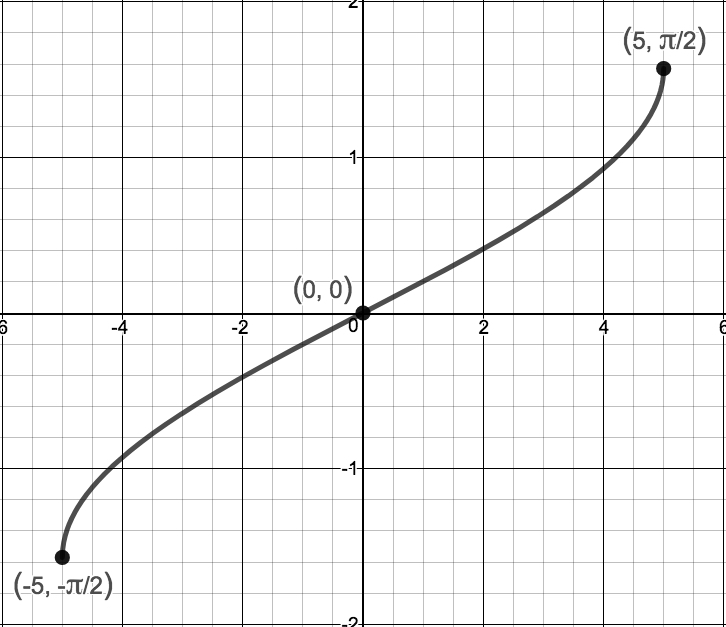
\includegraphics[height = 1.8in]{./TheInverseTrigonometricFunctionsGraphics/arccosgraph.jpg}

 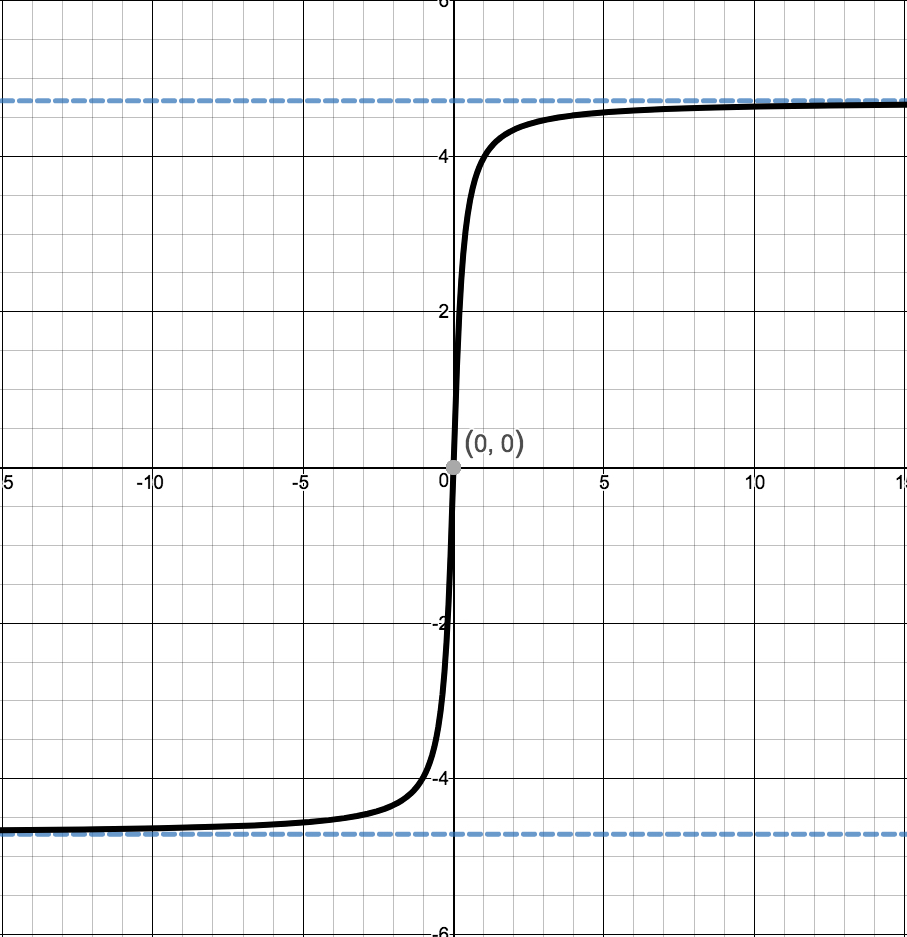
\includegraphics[height=1.81in]{./TheInverseTrigonometricFunctionsGraphics/arctangraph.jpg} 
 
 \end{multicols}

\begin{multicols}{2}

$y =f(x) = \frac{\pi}{2} - \arccos\left(\frac{x}{5}\right)$ 

$y = g(x) = 3\arctan\left(4x \right)$ \vphantom{$y =f(x) = \frac{\pi}{2} - \arccos\left(\frac{x}{5}\right)$ }

 \end{multicols}

\end{center}

\end{enumerate}

\end{enumerate}

\qed
\end{ex}

\subsection{Solving Equations Using the Inverse Trigonometric Functions.}

In Sections \ref{TheCircularFunctionsSineandCosine} and \ref{TheOtherCircularFunctions}, we learned how to solve equations like $\sin(\theta) = \frac{1}{2}$  and $\tan(t) = -1$. In each case, we ultimately appealed to the Unit Circle and relied on the fact that the answers corresponded to a set of `common angles' listed on page \pageref{commonanglesunitcircle}. 

\smallskip

 If, on the other hand, we had been asked to find all angles with $\sin(\theta) = \frac{1}{3}$ or solve $\tan(t) = -2$ for real numbers $t$, we would have been hard-pressed to do so.  With the introduction of the inverse trigonometric functions, however, we are now in a position to solve these equations. 
 
 \smallskip
 
 A good parallel to keep in mind is how the square root function can be used to solve certain quadratic equations.  The equation $x^2 = 4$ is a lot like  $\sin(\theta) = \frac{1}{2}$ in that it has friendly, `common value' answers  $x = \pm 2$.   The equation $x^2 = 7$, on the other hand, is a lot like $\sin(\theta) = \frac{1}{3}$.  We know there are answers, but we can't express them using `friendly' numbers.  
 
 \smallskip
 
 To solve $x^2 = 7$, we make use of the square root function (which is an inverse to $f(x) = x^2$ on a restricted domain) and write our answer as  $x = \pm \sqrt{7}$.  We need  the $\pm$ to  adjust for the fact that $\sqrt{7}$ is defined to be positive only, but we know we have two solutions, one positive and one negative.    Using a  calculator, we can certainly \textit{approximate} the values $\pm \sqrt{7}$,  but as far as exact answers go, we leave them as $x = \pm \sqrt{7}$.  
  
  \smallskip
  
In the same way, we will use the arcsine function (the inverse to the sine function on a restricted domain)  to solve $\sin(\theta) = \frac{1}{3}$.  However, we will need to adjust for the fact that there is more than one answer to this equation (infinitely many, in fact!)  As it turns out, we will be able to express every solution in terms of $\arcsin\left(\frac{1}{3}\right)$, as our next example illustrates.

\begin{ex}  \label{basicinverseeqns}  Solve the following equations.

\begin{enumerate}

\item  \label{basicinverseeqnssine} Find all angles $\theta$ for which $\sin(\theta) = \frac{1}{3}$.

\item \label{basicinverseeqnstangent} Find all real numbers $t$ for which $\tan(t) = -2$

\item  \label{basicinverseeqnssecant} Solve $\, \sec(x) = -\frac{5}{3} \,$ for $x$.

\end{enumerate}

{\bf Solution.}  

\begin{enumerate}

\item  If $\sin(\theta) = \frac{1}{3}$, then the terminal side of $\theta$, when plotted in standard position, intersects the Unit Circle at $y = \frac{1}{3}$.  Geometrically, we see that this happens at two places:  in Quadrant I and Quadrant II. 

\smallskip

If we let $\alpha$ denote the acute solution to the equation, then all the solutions to this equation in Quadrant I  are coterminal with $\alpha$, and $\alpha$ serves as the reference angle for all of the solutions to this equation in Quadrant II as seen below.

\smallskip

Since $\frac{1}{3}$ isn't the sine of any of the `common angles' we've encountered, we use the arcsine functions to express our answers.  By definition,  real number $t = \arcsin\left(\frac{1}{3}\right)$  $\sin(t) = \frac{1}{3}$ with $0 < t < \frac{\pi}{2}$.  

\smallskip

Hence, $\alpha = \arcsin\left(\frac{1}{3}\right)$ radians is an acute angle with $\sin(\alpha) = \frac{1}{3}$. Since all of the Quadrant I solutions $\theta$  are all coterminal with $\alpha$, we get $\theta = \alpha + 2\pi k  = \arcsin\left(\frac{1}{3}\right) + 2\pi k$ for integers $k$. 

\smallskip

 Turning our attention to Quadrant II, we get one solution to be $\pi - \alpha$.  Hence, the Quadrant II solutions are  $\theta = \pi - \alpha + 2\pi k = \pi - \arcsin\left(\frac{1}{3}\right) + 2\pi k$, for integers $k$.

\begin{tabular}{cc}

\begin{mfpic}[18]{-5}{5}{-5}{5}
\axes
\tlabel(5,-0.5){\scriptsize $x$}
\tlabel(0.25,5){\scriptsize $y$}
\tlabel(3.1,-0.75){\scriptsize $1$}
\tlabel(0.25,3.1){\scriptsize $1$}
\xmarks{-3 step 3 until 3}
\ymarks{-3, 1, 3}
\tlpointsep{4pt}
\axislabels{y}{{\scriptsize $\frac{1}{3}$} 1}
\drawcolor[gray]{0.7}
\circle{(0,0),3}
\drawcolor{black}
\arrow \parafcn{5, 20, 5}{2.75*dir(t)}
\penwd{1.25pt}
\arrow \reverse \arrow \polyline{(5,0), (0,0), (4.532, 2.113)}
\tlabel[cc](5.5, 0.61){\scriptsize $\alpha = \arcsin\left(\frac{1}{3}\right)$ radians}
\end{mfpic}

&

\hspace{0.25in}

\begin{mfpic}[18]{-5}{5}{-5}{5}
\axes
\tlabel(5,-0.5){\scriptsize $x$}
\tlabel(0.25,5){\scriptsize $y$}
\tlabel(3.1,-0.75){\scriptsize $1$}
\tlabel(0.25,3.1){\scriptsize $1$}
\xmarks{-3 step 3 until 3}
\ymarks{-3, 1, 3}
\tlpointsep{4pt}
\axislabels{y}{{\scriptsize $\frac{1}{3}$} 1}
\drawcolor[gray]{0.7}
\circle{(0,0),3}
\drawcolor{black}
\arrow \reverse \arrow \parafcn{160, 175, 5}{2.75*dir(t)}
\gclear \tlabelrect[cc](0, 2.5){\scriptsize \mbox{$\pi$}}
\arrow  \parafcn{5, 175, 5}{2*dir(t)}
\penwd{1.25pt}
\arrow \reverse \arrow \polyline{(5,0), (0,0), (-4.532, 2.113)}
\tlabel[cc](-3.45, 0.61){\scriptsize $\alpha$}
\end{mfpic} \\

\end{tabular}


\item The real number solutions to $\tan(t)=-2$  correspond to angles $\theta$  with $\tan(\theta) = -2$.  Since tangent is negative only in Quadrants II and IV, we focus our efforts there. 

\smallskip

The real number $t = \arctan(-2)$ satisfies $\tan(t)=-2$  and $-\frac{\pi}{2} < t < 0$.   If we let $\beta = \arctan(-2)$ radians, then all of the Quadrant IV solutions to  $\tan(\theta) = -2$  are coterminal with $\beta$. 

\smallskip

Moreover, as seen below on the right, the solutions from Quadrant II differ by exactly $\pi$ units from the solutions in Quadrant IV (recall, the period  of the tangent function is $\pi$.)  Hence, all of the  solutions to $\tan(\theta) = -2$ are of the form $\theta = \beta + \pi k = \arctan(-2) + \pi k$ for some integer $k$.   Switching back to the variable $t$,  we record our final answer to $\tan(t) = -2$ as $t = \arctan(-2) + \pi k$ for integers $k$.

\begin{tabular}{cc}

\begin{mfpic}[18]{-5}{5}{-5}{5}
\axes
\tlabel(5,-0.5){\scriptsize $x$}
\tlabel(0.25,5){\scriptsize $y$}
\tlabel(3.1,0.25){\scriptsize $1$}
\tlabel(0.25,3.1){\scriptsize $1$}
\xmarks{-3 step 3 until 3}
\ymarks{-3 step 3 until 3}
\drawcolor[gray]{0.7}
\circle{(0,0),3}
\drawcolor{black}
\arrow \parafcn{355, 305, -5}{1.5*dir(t)}
\gclear \tlabelrect[cc](4, -1){\scriptsize $\beta = \arctan(-2)$ radians}
\penwd{1.25pt}
\arrow \reverse \arrow \polyline{(5,0), (0,0), (2.5, -4.3301)}
\end{mfpic}

&

\hspace{.25in}


\begin{mfpic}[18]{-5}{5}{-5}{5}
\axes
\tlabel(5,-0.5){\scriptsize $x$}
\tlabel(0.25,5){\scriptsize $y$}
\tlabel(3.1,0.25){\scriptsize $1$}
\tlabel(0.25,3.1){\scriptsize $1$}
\xmarks{-3 step 3 until 3}
\ymarks{-3 step 3 until 3}
\drawcolor[gray]{0.7}
\circle{(0,0),3}
\drawcolor{black}
\arrow \parafcn{355, 305, -5}{1.5*dir(t)}
\arrow \reverse \arrow \parafcn{125, 295, 5}{1.5*dir(t)}
\tlabel[cc](-2, -1){\scriptsize $\pi$}
\tlabel[cc](2, -1){\scriptsize $\beta$}
\penwd{1.25pt}
\arrow \reverse \arrow \polyline{(5,0), (0,0), (-2.5, 4.3301)}
\arrow \reverse \arrow \polyline{(5,0), (0,0), (2.5, -4.3301)}
\end{mfpic} \\

\end{tabular}

\smallskip

Another tact we could have taken to solve this problem is to use reference angles.  Consider the (angle) equation: $\tan(\theta) = -2$.  If we let $\alpha$ be the reference angle for the solutions $\theta$, we know $\alpha$ is an acute angle with $\tan(\alpha) = 2$.  

\smallskip

By definition, the real number $t = \arctan(2)$ satisfies $0 < t < \frac{\pi}{2}$ with $\tan(t) = 2$.  Hence, the angle $\alpha = \arctan(2)$ radians is the reference angle for our solutions to $\tan(\theta) = -2$.  

\smallskip

Adjusting for quadrants, we get our answers to $\tan(\theta) = -2$ are  $\theta = - \alpha + \pi k = -\arctan(2) + \pi k$ for integers $k$.   Again, we cosmetically change the variable from $\theta$ back to $t$ so our answer to $\tan(t) = -2$ is $t = -\arctan(2) + \pi k$.  Thanks to the odd property of arctangent,  $\arctan(-2) = -\arctan(2)$ and we see this family of solutions is identical to what we obtained earlier.

\begin{tabular}{cc}

\begin{mfpic}[18]{-5}{5}{-5}{5}
\axes
\tlabel(5,-0.5){\scriptsize $x$}
\tlabel(0.25,5){\scriptsize $y$}
\tlabel(3.1,-0.25){\scriptsize $1$}
\tlabel(0.25,3.1){\scriptsize $1$}
\xmarks{-3 step 3 until 3}
\ymarks{-3 step 3 until 3}
\drawcolor[gray]{0.7}
\circle{(0,0),3}
\drawcolor{black}
\arrow \parafcn{5, 55, 5}{1.5*dir(t)}
\gclear \tlabelrect[cc](4, 1){\scriptsize $\alpha = \arctan(2)$ radians}
\penwd{1.25pt}
\arrow \reverse \arrow \polyline{(5,0), (0,0), (2.5, 4.3301)}
\end{mfpic}

&

\hspace{.25in}


\begin{mfpic}[18]{-5}{5}{-5}{5}
\axes
\tlabel(5,-0.5){\scriptsize $x$}
\tlabel(0.25,5){\scriptsize $y$}
\tlabel(3.1,-0.25){\scriptsize $1$}
\tlabel(0.25,3.1){\scriptsize $1$}
\xmarks{-3 step 3 until 3}
\ymarks{-3 step 3 until 3}
\drawcolor[gray]{0.7}
\circle{(0,0),3}
\drawcolor{black}
\arrow \reverse \arrow \parafcn{355, 305, -5}{1.5*dir(t)}
\arrow \reverse \arrow \parafcn{125, 295, 5}{1.5*dir(t)}
\tlabel[cc](-2, -1){\scriptsize $\pi$}
\tlabel[cc](2, -1){\scriptsize $\alpha$}
\penwd{1.25pt}
\arrow \reverse \arrow \polyline{(5,0), (0,0), (-2.5, 4.3301)}
\arrow \reverse \arrow \polyline{(5,0), (0,0), (2.5, -4.3301)}
\end{mfpic} \\

\end{tabular}



\item  In the last equation, $\sec(x) = -\frac{5}{3}$, we are not told whether or not $x$ represents an angle or a real number.  This isn't really much of an issue, since we attack both problems the same way.  

\smallskip

Taking a cue from our work in Section \ref{TheOtherCircularFunctions} and use a Reciprocal Identity to convert the equation $\sec(x) = -\frac{5}{3}$ to   $\cos(x) = -\frac{3}{5}$.    Thinking geometrically,  we are looking for angles $\theta$ with  $\cos(\theta) = -\frac{3}{5}$.  Since $\cos(\theta) < 0$, we are looking for solutions in  Quadrants II and III.   Since $-\frac{3}{5}$ isn't  the cosine of any of the `common angles', we'll need to express our solutions in terms of the arccosine function.  


\begin{tabular}{cc}


\begin{mfpic}[18]{-5}{5}{-5}{5}
\axes
\tlabel(5,-0.5){\scriptsize $x$}
\tlabel(0.25,5){\scriptsize $y$}
\tlabel(3.1,-0.75){\scriptsize $1$}
\tlabel(0.25,3.1){\scriptsize $1$}
\xmarks{-3 step 3 until 3}
\ymarks{-3 step 3 until 3}
\drawcolor[gray]{0.7}
\circle{(0,0),3}
\drawcolor{black}
\arrow \parafcn{5, 115, 5}{1.5*dir(t)}
\gclear \tlabelrect[cc](4, 1.5){\scriptsize $\beta = \arccos\left(-\frac{3}{5}\right)$ radians}
\penwd{1.25pt}
\arrow \reverse \arrow \polyline{(5,0), (0,0), (-2.5, 4.3301)}
\end{mfpic}
&

\hspace{-.15in}

\begin{mfpic}[18]{-5}{5}{-5}{5}
\axes
\tlabel(5,-0.5){\scriptsize $x$}
\tlabel(0.25,5){\scriptsize $y$}
\tlabel(3.1,-0.75){\scriptsize $1$}
\tlabel(0.25,3.1){\scriptsize $1$}
\xmarks{-3 step 3 until 3}
\ymarks{-3 step 3 until 3}
\drawcolor[gray]{0.7}
\circle{(0,0),3}
\drawcolor{black}
\arrow \dotted \parafcn{5, 115, 5}{1.5*dir(t)}
\gclear \tlabelrect[cc](4, 1.5){\scriptsize $\beta = \arccos\left(-\frac{3}{5}\right)$ radians}
\arrow \parafcn{355, 245, -5}{1.5*dir(t)}
\dashed \polyline{ (0,0), (-2.5, 4.3301)}
\gclear \tlabelrect[cc](4, -1.5){\scriptsize $-\beta = -\arccos\left(-\frac{3}{5}\right)$ radians}
\penwd{1.25pt}
\arrow \reverse \arrow \polyline{(5,0), (0,0), (-2.5, -4.3301)}
\end{mfpic} \qed \\


\end{tabular}


The real number $t = \arccos\left(-\frac{3}{5}\right)$ is defined so that $\frac{\pi}{2} < t < \pi$ with $\cos(t) = -\frac{3}{5}$.  Hence, the angle $\beta = \arccos\left(-\frac{3}{5}\right)$ radians is a Quadrant II angle which satisfies $\cos(\beta) = -\frac{3}{5}$. To obtain a Quadrant III angle solution, we may simply use $-\beta = -\arccos\left(-\frac{3}{5}\right)$ as seen above on the right.

\smallskip

Since all angle solutions are coterminal with $\beta$ or $-\beta$, we get our solutions to $\cos(\theta) = -\frac{3}{5}$ to be $\theta = \beta + 2\pi k = \arccos\left(-\frac{3}{5}\right) + 2\pi k$ or $\theta = -\beta + 2\pi k = -\arccos\left(-\frac{3}{5}\right) + 2\pi k$ for integers $k$.  

\smallskip

Switching back to the variable $x$,  we record our final answer to $\sec(x) = -\frac{5}{3}$ as $x = \arccos\left(-\frac{3}{5}\right) + 2\pi k$ or $x = -\arccos\left(-\frac{3}{5}\right) + 2\pi k$ for integers $k$.


\smallskip

As with the previous problem, we can approach solving  $\cos(\theta) = -\frac{3}{5}$ using reference angles.  Letting $\alpha$ represent the reference angle for the solutions $\theta$, we know $\alpha$ is an acute angle with $\cos(\alpha) = \frac{3}{5}$.

\smallskip

We know the real number $t = \arccos\left( \frac{3}{5} \right)$ satisfies $\cos(t) = \frac{3}{5}$ and $0 < t < \frac{\pi}{2}$, hence $\alpha = \arccos\left( \frac{3}{5} \right)$ radians is the reference angle for the solutions to  $\cos(\theta) = -\frac{3}{5}$.

\smallskip

Hence, the Quadrant II solutions to $\cos(\theta) = -\frac{3}{5}$ are $\theta = \pi - \alpha + 2\pi k = \pi -  \arccos\left( \frac{3}{5} \right) + 2\pi k$  while the Quadrant IV solutions to $\cos(\theta) = -\frac{3}{5}$ are $\theta = \pi + \alpha + 2\pi k = \pi + \arccos\left( \frac{3}{5} \right) + 2\pi k$ for integers $k$.

\begin{tabular}{cc}


\begin{mfpic}[18]{-5}{5}{-5}{5}
\axes
\tlabel(5,-0.5){\scriptsize $x$}
\tlabel(0.25,5){\scriptsize $y$}
\tlabel(3.1,-0.75){\scriptsize $1$}
\tlabel(0.25,3.1){\scriptsize $1$}
\xmarks{-3 step 3 until 3}
\ymarks{-3 step 3 until 3}
\drawcolor[gray]{0.7}
\circle{(0,0),3}
\drawcolor{black}
\arrow \parafcn{5, 55, 5}{1.5*dir(t)}
\gclear \tlabelrect[cc](4, 1.5){\scriptsize $\alpha = \arccos\left(\frac{3}{5}\right)$ radians}
\penwd{1.25pt}
\arrow \reverse \arrow \polyline{(5,0), (0,0), (2.5, 4.3301)}
\end{mfpic}
&

\hspace{-.15in}

\begin{mfpic}[18]{-5}{5}{-5}{5}
\axes
\tlabel(5,-0.5){\scriptsize $x$}
\tlabel(0.25,5){\scriptsize $y$}
\tlabel(3.1,-0.75){\scriptsize $1$}
%\tlabel(0.25,3.1){\scriptsize $1$}
\xmarks{-3 step 3 until 3}
\ymarks{-3 step 3 until 3}
\drawcolor[gray]{0.7}
\circle{(0,0),3}
\drawcolor{black}
\arrow \parafcn{5, 115, 5}{1.25*dir(t)}
\gclear \tlabelrect[cc](0.75, 3){\scriptsize $\pi - \arccos\left(\frac{3}{5}\right)$ radians}
\arrow \parafcn{5, 235, -5}{dir(t)}
\gclear \tlabelrect[cc](0.75, -3){\scriptsize $\pi + \arccos\left(-\frac{3}{5}\right)$ radians}
\arrow \reverse \arrow \parafcn{185, 235, 5}{1.5*dir(t)}
\gclear \tlabelrect[cc](-4, 1){\scriptsize $\alpha = \arccos\left(\frac{3}{5}\right)$ radians}
\arrow \reverse \arrow \parafcn{125, 175, 5}{1.5*dir(t)}
\gclear \tlabelrect[cc](-4, -1){\scriptsize $\alpha = \arccos\left(\frac{3}{5}\right)$ radians}
\penwd{1.25pt}
\arrow \reverse \arrow \polyline{(5,0), (0,0), (-2.5, -4.3301)}
\arrow \reverse \arrow  \polyline{ (5,0), (0,0), (-2.5, 4.3301)}
\end{mfpic} \qed \\


\end{tabular}

Shifting back to the variable $x$, we get our solution to $\sec(x) = -\frac{5}{3}$ are $x =  \pi -  \arccos\left( \frac{3}{5} \right) + 2\pi k$ or $x = \pi + \arccos\left( \frac{3}{5} \right) + 2\pi k$ for integers $k$.  While these certainly look quite different than what we obtained before, $x = \arccos\left(-\frac{3}{5}\right) + 2\pi k$ or $x = -\arccos\left(-\frac{3}{5}\right) + 2\pi k$ for integers $k$, they are, in fact, equivalent.  To show this, we start with $\arccos\left(-\frac{3}{5} \right) = \pi - \arccos\left(\frac{3}{5} \right)$ and begin writing out specific solutions from each family by choosing specific values of $k$.  We leave these details to the reader.  \qed


\end{enumerate}

\end{ex}

\smallskip

We close this section with one last sinusoid example.

\begin{ex}  \label{expandedsinusoidinverseex}  Consider the function $f(t) = 3\cos(6t) -4 \sin(6t)$. Find a formula for $f(t)$:

\begin{enumerate}

\item  in the form $C(t) = A \cos(\omega t + \phi) + B$ for $\omega > 0$

\item  in the form $S(t) = A \sin(\omega t + \phi) + B$ for $\omega > 0$

\end{enumerate}

{\bf Solution.}  

\begin{enumerate}

\item As in Example \ref{expandedsinusoidex1}, we compare the expanded form of $C(t) = A \cos(\omega t) \cos(\phi) - A \sin(\omega t) \sin(\phi) + B$ with $f(t) = 3\cos(6t) -4 \sin(6t)$. We identify $\omega = 6$ and $B = 0$ and by equating coefficients of  $\cos(6t)$ and $\sin(6t)$  get the two equations: $A \cos(\phi) = 3$ and $A \sin(\phi) = 4$.

\smallskip

Using the Pythagorean Identity to eliminate $\phi$, we get $A^2 = (A \cos(\phi))^2 + (A \sin(\phi))^2 = 3^2 + 4^2 = 25$.  We choose $A = 5$ and work to find the phase angle $\phi$.

\smallskip

Substituting $A = 5$ into our two equations relating $A$ and $\phi$, we get $5 \cos(\phi) = 3$, or $\cos(\phi) = \frac{3}{5}$  and $5 \sin(\phi) = 4$, so $\sin(\phi) = \frac{4}{5}$.  Since both $\sin(\phi)$ and $\cos(\phi)$ are positive, we know $\phi$ is a Quadrant I angle.  However, since neither the sine nor cosine value of $\phi$ corresponds to a common angle, we need to express $\phi$ in terms of either an arcsine or arccosine.

\smallskip

Since the real number $t = \arccos\left(\frac{3}{5}\right)$ satisfies $\cos(t) = \frac{3}{5}$ and $0 < t < \frac{\pi}{2}$, we know the angle $\phi = \arccos\left(\frac{3}{5}\right)$ radians is an acute (Quadrant I) angle which satisfies $\cos(\phi) = \frac{3}{5}$.  Hence, we can take $\phi = \arccos\left(\frac{3}{5}\right)$ and write $f(t) = 5 \cos\left(6t + \arccos\left(\frac{3}{5}\right) \right)$.

\smallskip

In addition, the real number $t = \arcsin\left(\frac{4}{5}\right)$ satisfies $\sin(t) = \frac{4}{5}$ and $0 < t < \frac{\pi}{2}$.  Hence $\phi = \arcsin\left(\frac{4}{5}\right)$ radians is Quadrant I angle with  $\sin(\phi) = \frac{4}{5}$.  This means we could also take $\phi = \arcsin\left(\frac{4}{5}\right)$ and write $f(t) = 5 \cos\left(6t + \arcsin\left(\frac{4}{5}\right) \right)$.  (We could also express $\phi$ in terms of arctangents, if we wanted!)

\smallskip

We leave it to the reader to verify (both) solutions analytically and graphically.


\item Once again, we equate the expanded form of $S(t) = A \sin(\omega t) \cos(\phi) + A \cos(\omega t) \sin(\phi) + B$ with $f(t) = 3\cos(6t) -4 \sin(6t)$. Once again, we get  $\omega = 6$ and $B = 0$.  Here, our two equations for $A$ and $\phi$ are $A \cos(\phi) = -4$ and $A \sin(\phi) = 3$.

\smallskip

As before, we get $A^2 = (A \cos(\phi))^2 + (A \sin(\phi))^2 = (-4)^2 + 3^2 = 25$, and we choose $A = 5$. Our equations for $\phi$ become:  $\cos(\phi) = -\frac{4}{5}$ and $\sin(\phi) = \frac{3}{5}$.  Since $\cos(\phi)<0$ but $\sin(\phi) > 0$, we know $\phi$ is a Quadrant II angle. As before, since neither the sine nor cosine value of $\phi$ corresponds to a common angle, we need to express $\phi$ in terms of either an arcsine or arccosine.

\smallskip

Here, we opt to use the arccosine function, since the range of arccosine, $[0, \pi]$ covers Quadrant II.   From  $\cos(\phi) = -\frac{4}{5}$ , we get $\phi = \arccos\left(-\frac{4}{5}\right)$, so $f(t) = 5 \sin\left(6t + \arccos\left(-\frac{4}{5}\right) \right)$.  

\smallskip

Had we chosen to work with arcsines, we would need a Quadrant II solution to $\sin(\phi) = \frac{3}{5}$.  Going through the usual machinations, we arrive at $\phi = \pi - \arcsin\left( \frac{3}{5} \right)$.  Hence, an alternative form of our answer is $f(t) = 5 \sin \left( 6t +  \pi - \arcsin\left( \frac{3}{5} \right) \right)$.  We leave the checks to the reader.  \qed

\end{enumerate}


\end{ex}


\newpage
\subsection{Exercises}

\input{ExercisesforTheInverseTrigonometricFunctions}

\closegraphsfile

\newpage

\section{Equations and Inequalities Involving the Circular Functions}

\mfpicnumber{1}

\opengraphsfile{TrigonometricEquationsandInequalities}

\setcounter{footnote}{0}

\label{TrigonometricEquationsandInequalities}

In Sections \ref{TheCircularFunctionsSineandCosine}, \ref{TheOtherCircularFunctions} and most recently \ref{TheInverseTrigonometricFunctions}, we solved some basic equations involving the trigonometric functions. Below we summarize the techniques we've employed thus far.  Note that we use the neutral letter `$u$' as the argument of each circular function for generality.

\smallskip

\phantomsection
\label{trigeqnstrategy1}

\colorbox{ResultColor}{\bbm
\centerline{\textbf{Strategies for Solving Basic Equations Involving the Circular Functions}}

\smallskip

\begin{itemize}

\item To solve $\cos(u) = c$ or $\sin(u) = c$ for $-1 \leq c \leq 1$, first solve for $u$ in the interval $[0,2\pi)$ and add integer multiples of the period $2\pi$.  If $c < -1$ or of $c > 1$, there are no real solutions.

\item To solve $\sec(u) = c$ or $\csc(u) = c$ for $c \leq -1$ or $c \geq 1$,  convert to cosine or sine, respectively, and solve as above.  If $-1 < c < 1$, there are no real solutions.

\item To solve  $\tan(u) = c$ for any real number $c$,  first solve for $u$ in the interval $\left(-\frac{\pi}{2}, \frac{\pi}{2}\right)$ and add integer multiples of the period $\pi$.

\item  To solve  $\cot(u) = c$ for $c \neq 0$, convert to tangent and solve as above.  If $c = 0$, the solution to $\cot(u) = 0$ is $u = \frac{\pi}{2} + \pi k$ for integers $k$.

\end{itemize}

\smallskip

\ebm}

\smallskip

Using the above guidelines, we can comfortably solve $\sin(x) = \frac{1}{2}$ and find the solution $x = \frac{\pi}{6} + 2\pi k$ or $x = \frac{5\pi}{6} + 2\pi k$ for integers $k$.  But how do we solve the related equation $\sin(3x) = \frac{1}{2}$?

\smallskip

 Since this equation has the \textit{form} $\sin(u) = \frac{1}{2}$, we know the solutions take the form  $u= \frac{\pi}{6} + 2\pi k$ or $u = \frac{5\pi}{6} + 2\pi k$ for integers $k$. Since the argument of sine here is $3x$, we have $3x= \frac{\pi}{6} + 2\pi k$ or $3x = \frac{5\pi}{6} + 2\pi k$.
 
 \smallskip
 
 To solve for $x$, we divide both sides\footnote{Don't forget to divide the $2\pi k$ by $3$ as well!} of these equations by $3$, and obtain $x = \frac{\pi}{18} + \frac{2\pi}{3} k$ or $x = \frac{5\pi}{18} + \frac{2\pi}{3}k$ for integers $k$.  This is the technique employed in the example below.

\begin{ex}  \label{TrigEqnEx1} Solve the following equations and check your answers analytically.  List the solutions which lie in the interval $[0,2\pi)$ and verify them using a graphing utility.


\begin{multicols}{3}

\begin{enumerate}

\item  $\cos(2\theta) = -\frac{\sqrt{3}}{2}$
\item  $\csc\left(\frac{1}{3}\theta-\pi \right) = \sqrt{2}$
\item  $\cot\left(3t \right) = 0$

\setcounter{HW}{\value{enumi}}

\end{enumerate}

\end{multicols}

\begin{multicols}{3} 

\begin{enumerate}

\setcounter{enumi}{\value{HW}}

\item  $\sec^{2}(t) = 4$
\item  \label{arctanin02pi} $\tan\left(\frac{x}{2}\right) = -3$
\item  $\sin(2x) = 0.87$

\end{enumerate}

\end{multicols}

{\bf Solution.}

\begin{enumerate}

\item  The solutions to $\cos(u) =-\frac{\sqrt{3}}{2}$ are $u = \frac{5\pi}{6} + 2\pi k$ or $u = \frac{7\pi}{6} + 2\pi k$ for integers $k$.  

\smallskip

Since the argument of cosine here is $2\theta$, this means $2\theta = \frac{5\pi}{6} + 2\pi k$ or $2\theta = \frac{7\pi}{6} + 2\pi k$ for integers $k$.  Solving for $\theta$ gives $\theta = \frac{5\pi}{12} + \pi k$ or $\theta = \frac{7\pi}{12} + \pi k$ for integers $k$. 

\smallskip

 To check these answers analytically, we substitute them into the original equation.  For any integer $k$:

\[ \begin{array}{rclr}

\cos\left( 2\left[\frac{5\pi}{12} + \pi k\right]\right) &  = &  \cos\left(\frac{5\pi}{6} + 2\pi k\right) & \\ [3pt]
																												& =  &   \cos\left(\frac{5\pi}{6}\right) & \text{(the period of cosine is $2\pi$)} \\ [3pt]
																												& =  & -\frac{\sqrt{3}}{2} & \\
\end{array}\] 

Similarly, we find $\cos\left( 2\left[\frac{7\pi}{12} + \pi k\right]\right) = \cos\left(\frac{7\pi}{6} + 2\pi k\right) = \cos\left(\frac{7\pi}{6}\right) = -\frac{\sqrt{3}}{2}$.  

\smallskip

To determine which of our solutions lie in $[0,2\pi)$, we substitute integer values for $k$.  The solutions we keep come from the values of $k = 0$ and $k =1$ and are  $\theta = \frac{5\pi}{12}$,  $\frac{7\pi}{12}$, $\frac{17\pi}{12}$ and $\frac{19\pi}{12}$.  

\smallskip

Using a calculator, we graph $y = \cos(2\theta)$ and $y = -\frac{\sqrt{3}}{2}$ over $[0,2\pi)$ and examine where these two graphs intersect to verify our answers.

\begin{center}

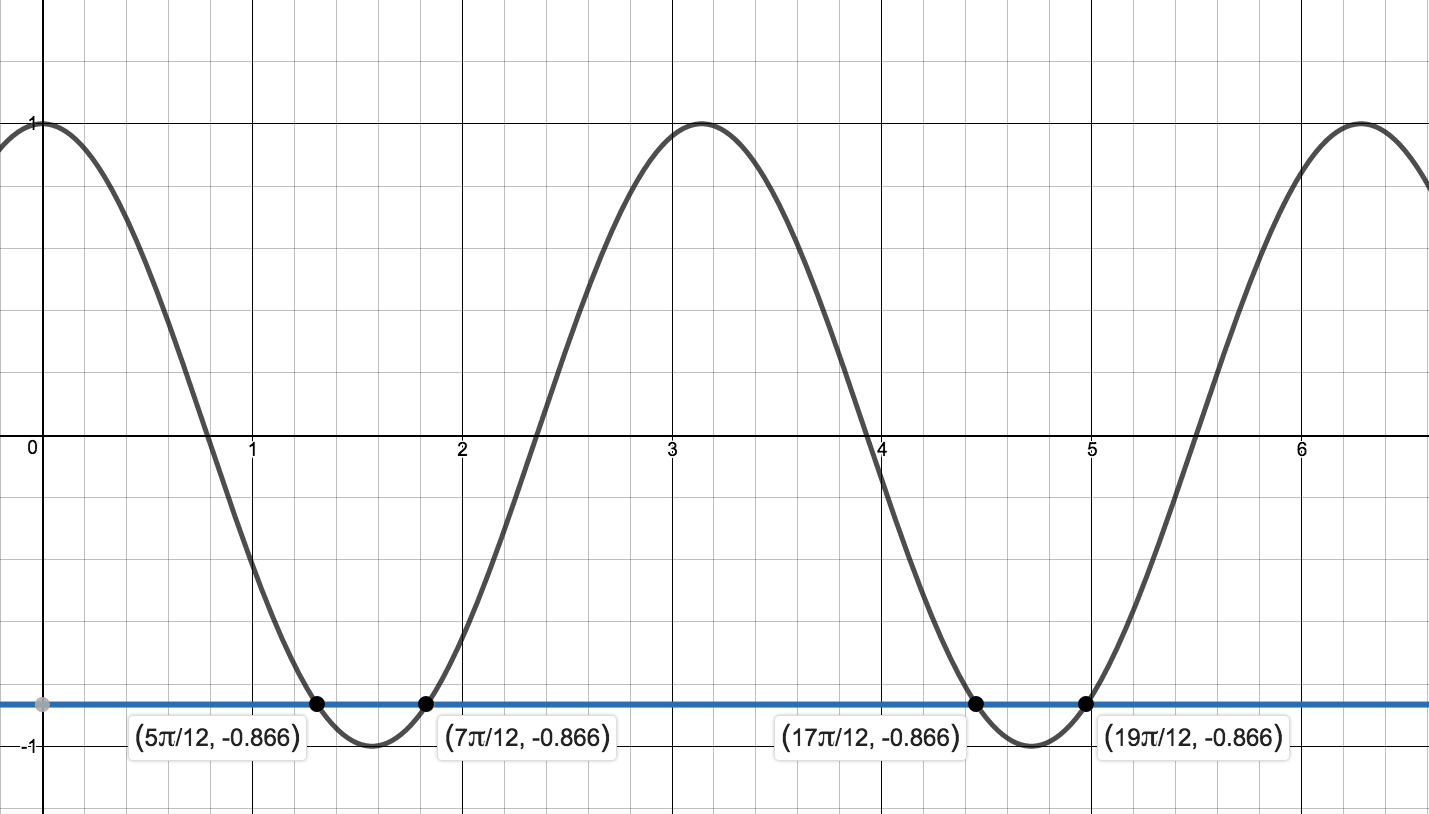
\includegraphics[height=2.25in]{./TrigonometricEquationsandInequalitiesGraphics/TrigEquIneq01.jpg}

{\boldmath $y = \cos(2\theta)$} and $y=-\frac{\sqrt{3}}{2}$

\end{center}


\item  Since this equation has the form $\csc(u) = \sqrt{2}$, we rewrite this as $\sin(u) = \frac{\sqrt{2}}{2}$ and find $u = \frac{\pi}{4} + 2\pi k$ or $u = \frac{3\pi}{4} + 2\pi  k$ for integers $k$.  

\smallskip

Since the argument of cosecant here is $\left(\frac{1}{3}\theta-\pi \right)$,  $\frac{1}{3}\theta-\pi = \frac{\pi}{4} + 2\pi k$ or $\frac{1}{3}\theta - \pi = \frac{3\pi}{4} + 2\pi k$.

\smallskip

To solve $\frac{1}{3} \theta-\pi = \frac{\pi}{4} + 2\pi k$, we first add $\pi$ to both sides to get  $\frac{1}{3} \theta = \frac{\pi}{4} + 2\pi k + \pi$. A common error is to treat the `$2\pi k$' and `$\pi$' terms as `like' terms and try to combine them when they are not.  

\smallskip

We can, however, combine the `$\pi$' and `$\frac{\pi}{4}$' terms to get $\frac{1}{3} \theta = \frac{5\pi}{4} + 2\pi k$.

\smallskip

We now finish by multiplying both sides by $3$ to get  $\theta  = 3 \left( \frac{5\pi}{4} + 2\pi k \right) = \frac{15 \pi}{4} + 6\pi k$, where $k$, as always, runs through the integers.

\smallskip

Solving the other equation, $\frac{1}{3} \theta-\pi = \frac{3\pi}{4} + 2\pi k$ produces $\theta = \frac{21\pi}{4} + 6 \pi k$ for integers $k$. To check the first family of answers, we substitute, combine line terms, and simplify.

\[ \begin{array}{rclr}

\csc\left(\frac{1}{3} \left[ \frac{15\pi}{4} + 6 \pi  k \right] - \pi   \right)  &  = &  \csc\left(\frac{5\pi}{4} + 2\pi k - \pi \right) & \\ [3pt]
																												& =  &   \csc\left(\frac{\pi}{4} + 2\pi k\right) &  \\ [3pt]
																												& =  & \csc\left(\frac{\pi}{4}\right) & \text{(the period of cosecant is $2\pi$)} \\
																												& = & \sqrt{2} & \\
\end{array}\] 



The family $\theta = \frac{21\pi}{4} + 6 \pi  k$ checks similarly. 

\smallskip

 Despite having infinitely many solutions, we find that \textit{none} of them lie in $[0,2\pi)$. 
 
 \smallskip
 
To verify this graphically, we check that $y = \csc\left(\frac{1}{3} \theta -\pi\right)$ and $y =\sqrt{2}$ do not intersect at all over the interval $[0,2\pi)$.


\begin{center}

 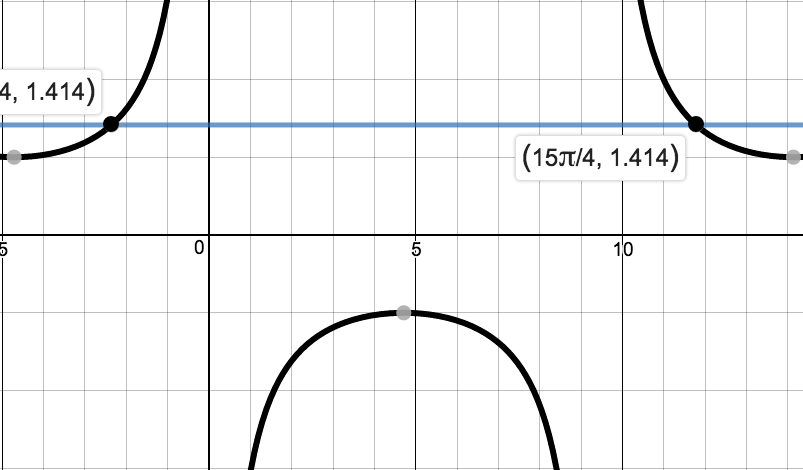
\includegraphics[height=2.25in]{./TrigonometricEquationsandInequalitiesGraphics/TrigEquIneq02.jpg} \\


{\boldmath  $y = \csc\left(\frac{1}{3} \theta -\pi\right)$} and $y =\sqrt{2}$ \\
 


\end{center}

\item  Since $\cot(3t) = 0$ has the form $\cot(u) = 0$, we know $u = \frac{\pi}{2} + \pi k$, so, in this case,  $3t =  \frac{\pi}{2} + \pi k$ for integers $k$.  

\smallskip

Solving for $t$ yields $t = \frac{\pi}{6} + \frac{\pi}{3} k$.  Checking our answers, we get

\[ \begin{array}{rclr}

\cot\left(3\left[ \frac{\pi}{6} + \frac{\pi}{3} k\right]\right)  &  = &  \cot\left(\frac{\pi}{2} + \pi k\right)  & \\ [3pt]
																												& =  &   \cot\left(\frac{\pi}{2}\right) &  \text{(the period of cotangent is $\pi$)} \\ [3pt]
																												& =  & 0 & \\
																								
\end{array}\] 

 As $k$ runs through the integers, we obtain six answers, corresponding to $k=0$ through $k=5$, which lie in $[0, 2\pi)$: $x = \frac{\pi}{6}$, $\frac{\pi}{2}$, $\frac{5\pi}{6}$, $\frac{7\pi}{6}$ , $\frac{3\pi}{2}$ and  $\frac{11\pi}{6}$. 
 
 \smallskip
 
 Graphing $y = \cot(3t)$ and $y=0$ (the $t$-axis), we confirm our result.\footnote{On many calculators, there is no function button for cotangent.  In that case, we would use the quotient identity and graph $y = \frac{\cos(3t)}{\sin(3t)}$ instead.  The reader is invited to see what happens if we would graph $y= \frac{1}{\tan(3t)}$ instead.}
 
 \begin{center}
 
 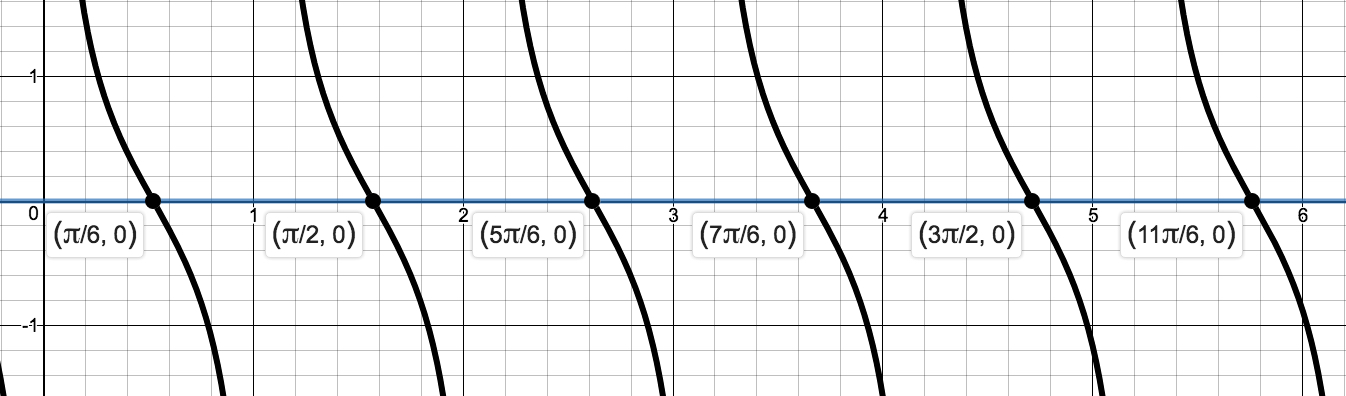
\includegraphics[height=1.75in]{./TrigonometricEquationsandInequalitiesGraphics/TrigEquIneq03.jpg} 
 
 { \boldmath $y = \cot(3t)$}  and $y=0$ 
 
 \end{center}

\item The complication in solving an equation like $\sec^{2}(t) = 4$ comes not from the argument of secant, which is just $t$, but rather, the fact the secant is being squared:  $\sec^{2}(t) = (\sec(t))^2 = 4$.

\smallskip

To get this equation to look like one of the forms listed on page \pageref{trigeqnstrategy1}, we extract square roots to get $\sec(t) = \pm 2$. Converting to cosines, we have  $\cos(t) = \pm \frac{1}{2}$.  

\smallskip

For $\cos(t) = \frac{1}{2}$, we get $t = \frac{\pi}{3} + 2\pi k$ or $t = \frac{5\pi}{3} + 2\pi k$ for integers $k$.  For $\cos(t) = -\frac{1}{2}$, we get $t = \frac{2\pi}{3} + 2\pi k$ or $t = \frac{4\pi}{3} + 2\pi k$ for integers $k$. 

\smallskip

If we take a step back and think of these families of solutions geometrically, we see we are finding the measures of all angles with a reference angle of $\frac{\pi}{3}$.  As a result, these solutions can be combined and we may write our solutions as $t = \frac{\pi}{3} + \pi k$ and $t = \frac{2\pi}{3} + \pi k$ for integers $k$. 

\smallskip

To check the first family of solutions, we note that, depending on the integer $k$,  $\sec\left(\frac{\pi}{3} + \pi k\right)$ doesn't always equal $\sec\left(\frac{\pi}{3}\right)$.  It is true, though,  that for all integers $k$,  $\sec\left(\frac{\pi}{3} + \pi k\right) = \pm \sec\left(\frac{\pi}{3}\right) = \pm 2$.  (Can you show this?)  Hence, checking our first family of solutions gives:


\[ \begin{array}{rclr}

\sec^{2}\left(\frac{\pi}{3} + \pi k\right)  &  = &  \left( \pm \sec\left(\frac{\pi}{3}\right)\right)^2  & \\ [3pt]
																												& =  &   (\pm 2)^2 &  \\ [3pt]
																												& =  & 4 & \\
																								
\end{array}\] 

The check for the family of solutions $t =\frac{2\pi}{3} + \pi k$ is similar. 

\smallskip

 The solutions which lie in $[0,2\pi)$ come from the values $k = 0$ and $k=1$, namely $t = \frac{\pi}{3}$, $\frac{2\pi}{3}$, $\frac{4\pi}{3}$ and $\frac{5\pi}{3}$.  Graphing $y = (\sec(t))^2$ and $y=4$ confirms our results.  

\begin{center}


 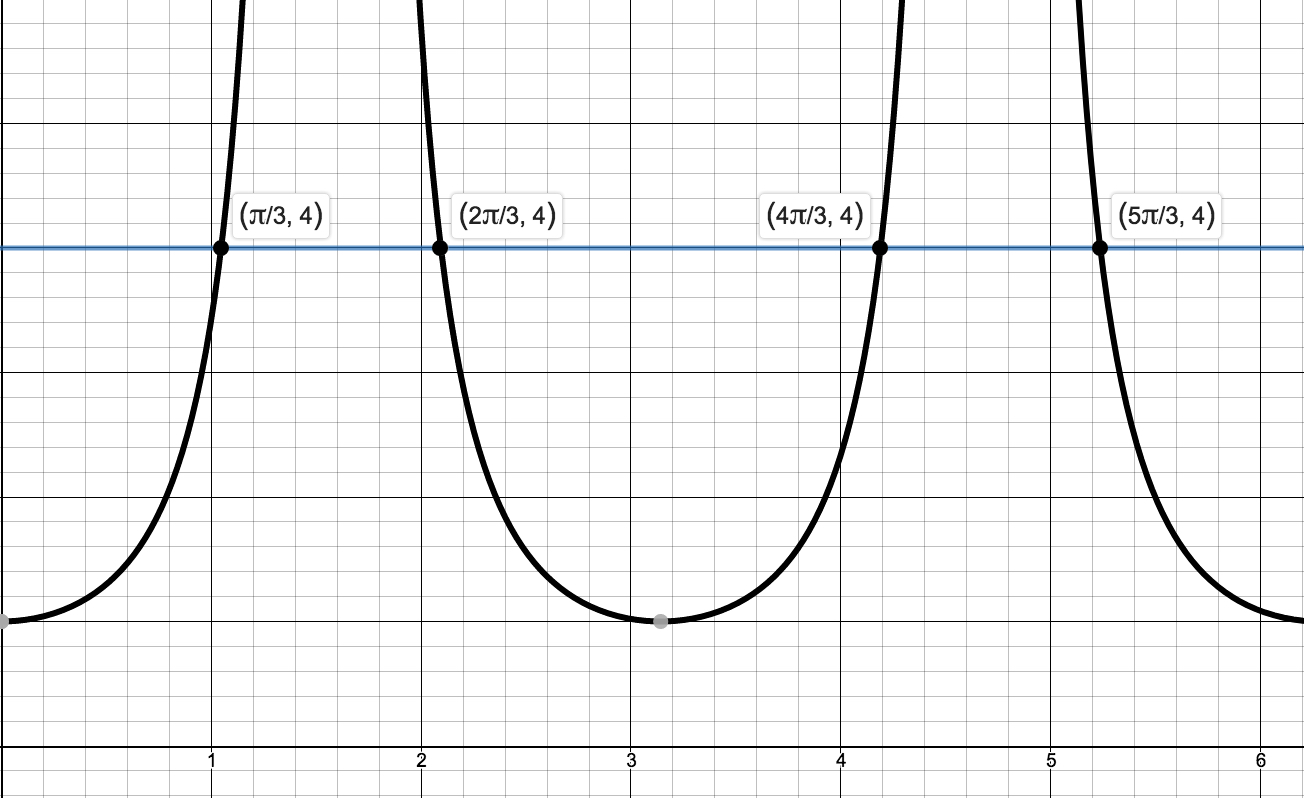
\includegraphics[height=2.25in]{./TrigonometricEquationsandInequalitiesGraphics/TrigEquIneq04.jpg} 

  {\boldmath $y = (\sec(t))^2$} and  $y = 4$  



\end{center}

\item  The equation  $\tan\left(\frac{x}{2}\right) = -3$ has the form $\tan(u) = -3$, whose solution is $u = \arctan(-3) + \pi k$.  

\smallskip

Hence, $\frac{x}{2} = \arctan(-3) + \pi k$, so  $x = 2\arctan(-3) + 2\pi k$ for integers $k$.  To check, we note

\[ \begin{array}{rclr}

\tan\left(\frac{2\arctan(-3) + 2\pi k}{2}\right)  &  = & \tan\left( \arctan(-3) + \pi k \right)  & \\ [3pt]
																												& =  & \tan\left(\arctan(-3) \right) & \text{(the period of tangent is $\pi$)} \\ [3pt]
																												& =  & -3 & (\text{See Theorem } \ref{arctangentcotangentfunctionprops}) \\
																								
\end{array}\] 


 To determine which of our answers lie in the interval $[0,2\pi)$, we first need to get an idea of the value of $2\arctan(-3)$.  While we could easily find an approximation using a calculator,\footnote{Your instructor will let you know if you should abandon the analytic route at this point and use your calculator.} we proceed analytically, as is our custom.
 
 \smallskip
 
To get started, we note that since $-3 < 0$, it  $-\frac{\pi}{2} < \arctan(-3) < 0$.  Hence,  $-\pi < 2\arctan(-3) < 0$.   With regard to our solutions,  $x = 2\arctan(-3) + 2\pi k$, we see for $k = 0$, we get $x = 2\arctan(-3) < 0$, so we discard this answer and all answers $x = 2\arctan(-3) + 2\pi k$ where $k < 0$.  

\smallskip

Next, we turn our attention to $k = 1$ and get $x = 2\arctan(-3) + 2\pi$. Starting with the inequality $-\pi < 2\arctan(-3) < 0$, we add through $2\pi$  and get $\pi < 2\arctan(-3) +2\pi < 2\pi$.  This means $x = 2\arctan(-3) + 2\pi$ lies in $[0,2\pi)$.  

\smallskip

Advancing $k$ to $2$ produces $x = 2\arctan(-3) + 4\pi$. Once again, we get from $-\pi < 2\arctan(-3) < 0$ that $3\pi < 2\arctan(-3) + 4\pi < 4\pi$.  Since this is outside the interval of interest, $[0,2\pi)$,  we discard $x = 2\arctan(-3) + 4\pi$ and all solutions of the form $x = 2\arctan(-3) + 2\pi k$ for $k > 2$.   

\smallskip

Graphically, $y = \tan\left(\frac{x}{2}\right)$ and $y = -3$ intersect only once on $[0,2\pi)$ at $x = 2\arctan(-3) + 2\pi\approx 3.785$.

\smallskip

\begin{center}


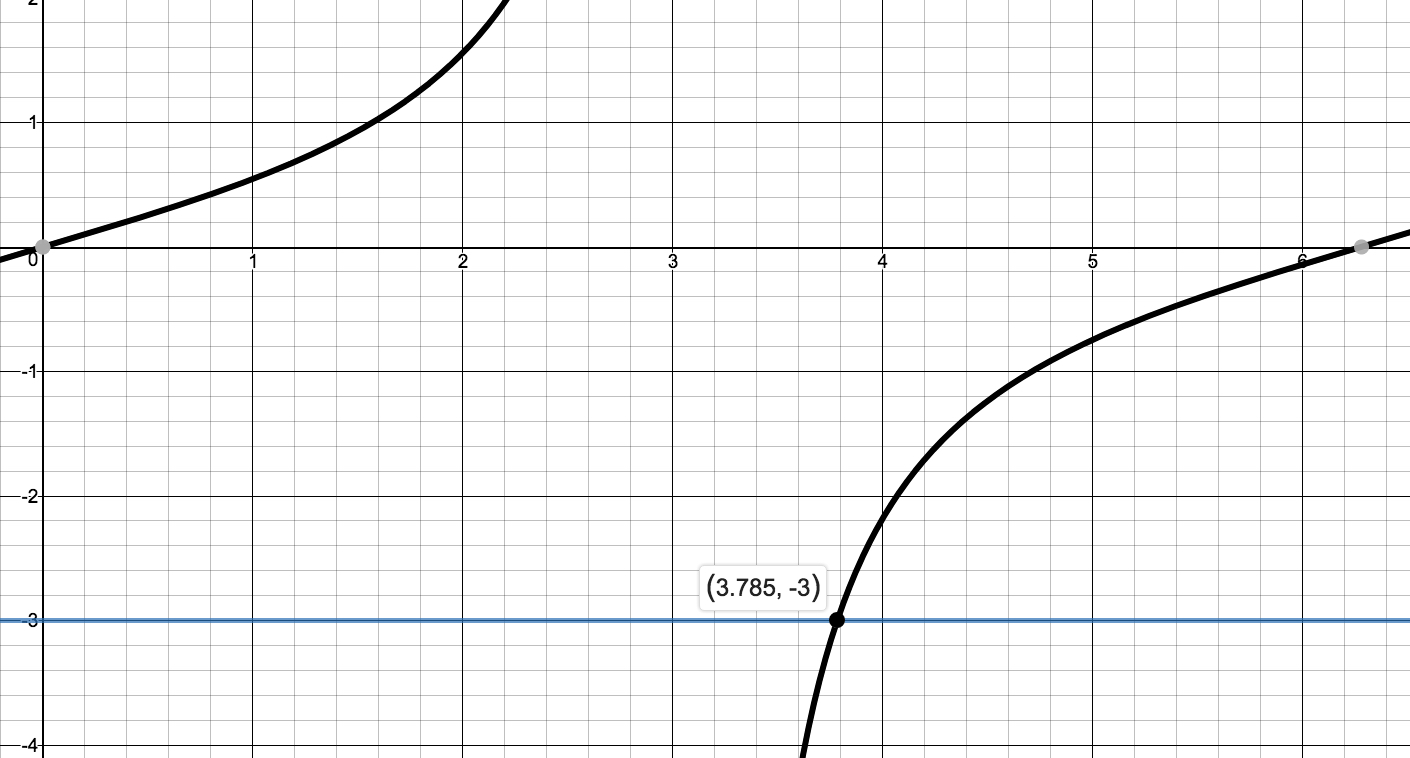
\includegraphics[height=2.25in]{./TrigonometricEquationsandInequalitiesGraphics/TrigEquIneq05.jpg}

{ \boldmath $y = \tan\left(\frac{x}{2}\right)$} and  $y = -3$ 

\end{center}

\item To solve $\sin(2x) = 0.87$, we first note that it has the form $\sin(u) = 0.87$, which has the family of solutions $u = \arcsin(0.87) + 2\pi k$ or $u =\pi -  \arcsin(0.87) + 2\pi k$ for integers $k$. 

\smallskip

Since the argument of sine here is $2x$, we get $2x = \arcsin(0.87) + 2\pi k$ or $2x =\pi -  \arcsin(0.87) + 2\pi k$ which gives $x = \frac{1}{2} \arcsin(0.87) + \pi k$ or $x =\frac{\pi}{2} -  \frac{1}{2}\arcsin(0.87) + \pi k$ for integers $k$.  To check,

\[ \begin{array}{rclr}

\sin\left(2\left[\frac{1}{2} \arcsin(0.87) + \pi k\right]\right)  &  = & \sin\left(\arcsin(0.87) + 2\pi k\right)  & \\ [3pt]
																													& =  & \sin\left(\arcsin(0.87)\right) & \text{(the period of sine is $2\pi$)} \\ [3pt]
																												& =  & 0.87& (\text{See Theorem } \ref{arccosinesinefunctionprops})\\
																								
\end{array}\] 


For the family $x =\frac{\pi}{2} -  \frac{1}{2}\arcsin(0.87) + \pi k$ , we get

\[ \begin{array}{rclr}

\sin\left(2\left[\frac{\pi}{2} - \frac{1}{2} \arcsin(0.87) + \pi k\right]\right)  &  = & \sin\left(\pi - \arcsin(0.87) + 2\pi k\right) & \\ [3pt]
																												& =  & \sin\left(\pi - \arcsin(0.87)\right) & \text{(the period of sine is $2\pi$)} \\ [3pt]
																												& =  & \sin\left(\arcsin(0.87)\right) & \text{($\sin(\pi - t) = \sin(t)$)} \\ [3pt]
																												& =  & 0.87& (\text{See Theorem } \ref{arccosinesinefunctionprops}) \\
																								
\end{array}\] 

To determine which of these solutions lie in $[0,2\pi)$, we first need to get an idea of the value of $x=\frac{1}{2} \arcsin(0.87)$.  Once again, we could use the calculator, but we adopt an analytic route here.  

\smallskip

By definition, $0 < \arcsin(0.87) < \frac{\pi}{2}$ so that multiplying through by $\frac{1}{2}$ gives us $0 < \frac{1}{2} \arcsin(0.87) < \frac{\pi}{4}$.  

\smallskip

Starting with the family of solutions $x = \frac{1}{2} \arcsin(0.87) + \pi k$, we use the same kind of arguments as in our solution to number \ref{arctanin02pi} above and find only the solutions corresponding to $k =0$ and $k=1$ lie in $[0,2\pi)$:  $x = \frac{1}{2} \arcsin(0.87)$ and $x = \frac{1}{2} \arcsin(0.87) + \pi$. 

\smallskip

 Next, we move to the family $x =\frac{\pi}{2} -  \frac{1}{2}\arcsin(0.87) + \pi k$ for integers $k$. Here, we need to get a better estimate of $\frac{\pi}{2} - \frac{1}{2} \arcsin(0.87)$.  From the inequality $0 < \frac{1}{2}\arcsin(0.87) < \frac{\pi}{4}$, we first multiply through by $-1$ and then add $\frac{\pi}{2}$ to get $\frac{\pi}{2} > \frac{\pi}{2} -\frac{1}{2} \arcsin(0.87) >  \frac{\pi}{4}$, or $\frac{\pi}{4} < \frac{\pi}{2} -\frac{1}{2} \arcsin(0.87) < \frac{\pi}{2}$.  
 
 \smallskip
 
 Proceeding with the usual arguments, we find the only solutions which lie in $[0,2\pi)$ correspond to $k = 0$ and $k=1$, namely $x =\frac{\pi}{2} -  \frac{1}{2}\arcsin(0.87)$ and  $x = \frac{3\pi}{2} - \frac{1}{2}\arcsin(0.87)$. 
 
 \smallskip
 
All told, we have found four solutions to $\sin(2x) = 0.87$ in $[0,2\pi)$:  $x =\frac{1}{2} \arcsin(0.87) \approx 0.528$, $x=\frac{1}{2} \arcsin(0.87) + \pi \approx 3.669$, $x =\frac{\pi}{2} -  \frac{1}{2}\arcsin(0.87) \approx 1.043$ and  $x = \frac{3\pi}{2} - \frac{1}{2}\arcsin(0.87) \approx 4.185$. By graphing $y = \sin(2x)$ and $y = 0.87$, we confirm our results.



\begin{center}


  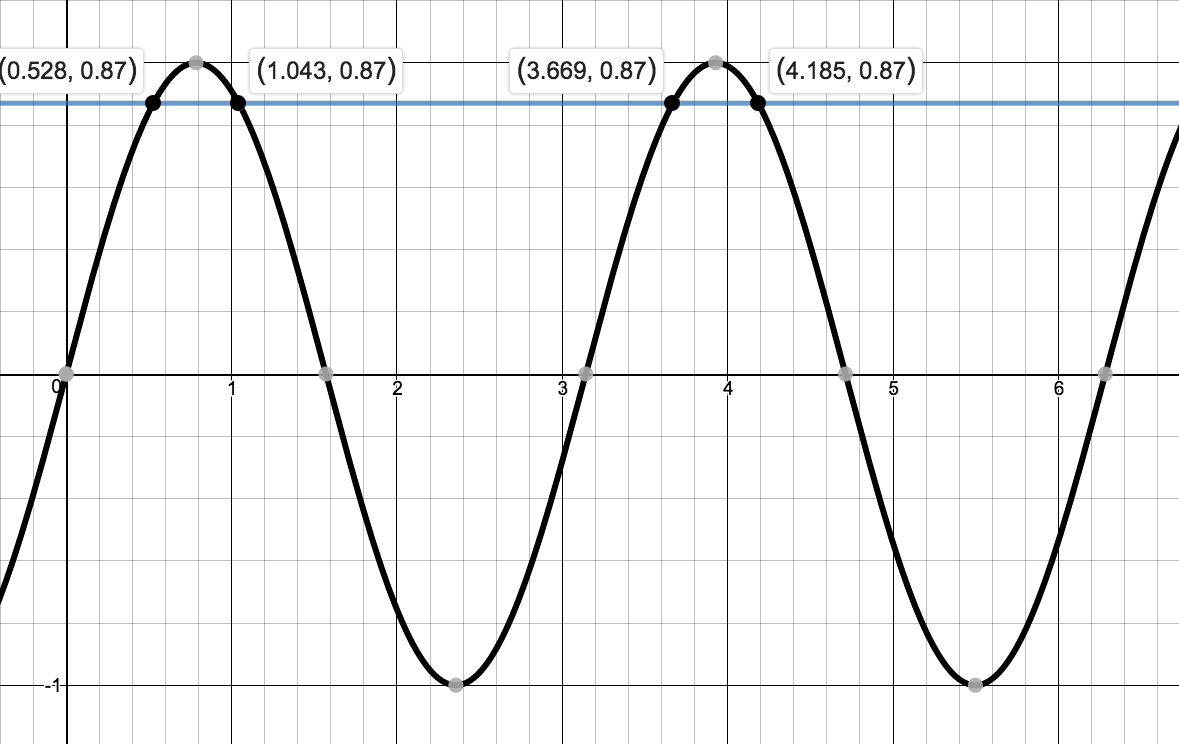
\includegraphics[height=2.25in]{./TrigonometricEquationsandInequalitiesGraphics/TrigEquIneq06.jpg} 

{\boldmath $y = \sin(2x)$} and  $y = 0.87$


\end{center} 

\end{enumerate}

\vspace*{-.3in} \qed

\end{ex}


If one looks closely at the equations and solutions in Example \ref{TrigEqnEx1}, an interesting relationship evolves between the frequency of the circular function involved in the equation and how many solutions one can expect in the interval $[0, 2\pi)$.   This relationship is explored in Exercise \ref{frequencynumberconnection}.

\smallskip

Each of the problems in Example \ref{TrigEqnEx1} featured one circular function.  If an equation involves two different circular functions or if the equation contains the same circular function but with different arguments, we will need to employ identities and Algebra to reduce the equation to the same form as those given on page  \pageref{trigeqnstrategy1}.  We demonstrate these techniques in the following example.
 
\begin{ex} \label{TrigEqIdEx1}  Solve the following equations and list the solutions which lie in the interval $[0,2\pi)$.  Verify your solutions on $[0,2\pi)$ graphically.

\begin{multicols}{2}

\begin{enumerate}

\item  $3\sin^{3}(\theta) = \sin^{2}(\theta)$
\item $\sec^{2}(\theta) = \tan(\theta) + 3$

\setcounter{HW}{\value{enumi}}

\end{enumerate}

\end{multicols}

\begin{multicols}{2}

\begin{enumerate}

\setcounter{enumi}{\value{HW}}

\item   $\cos(2t) = 3\cos(t) - 2$
\item  $\cos(3t) = 2- \cos(t)$

\setcounter{HW}{\value{enumi}}

\end{enumerate}

\end{multicols}

\begin{multicols}{2}

\begin{enumerate}

\setcounter{enumi}{\value{HW}}

\item  $\cos(3x) = \cos(5x)$
\item $\sin(2x) =\sqrt{3} \cos(x)$

\setcounter{HW}{\value{enumi}}

\end{enumerate}

\end{multicols}

\begin{multicols}{2}

\begin{enumerate}

\setcounter{enumi}{\value{HW}}

\item  $\sin(x)\cos\left(\frac{x}{2}\right) + \cos(x)\sin\left(\frac{x}{2}\right) = 1$
\item  $\cos(x) - \sqrt{3} \sin(x) = 2$

\end{enumerate}
 
\end{multicols}

\newpage

{\bf Solution.}

\begin{enumerate}

\item One approach to solving  $3\sin^{3}(\theta) = \sin^{2}(\theta)$ begins with dividing both sides by $\sin^{2}(\theta)$.  Doing so, however, assumes that $\sin^{2}(\theta) \neq 0$ which means we risk losing solutions.  

\smallskip

Instead, we take a cue from Chapter \ref{PolynomialFunctions} (since what we have here is a polynomial equation in terms of $\sin(\theta)$) and gather all the nonzero terms on one side and factor:
\[ \begin{array}{rclr}

3\sin^{3}(\theta) & = &  \sin^{2}(\theta) & \\
3\sin^{3}(\theta) -  \sin^{2}(\theta) & = & 0 &  \\
\sin^{2}(\theta) (3 \sin(\theta) - 1) & = & 0 & \text{Factor out $\sin^{2}(\theta)$ from both terms.} \\ \end{array} \]

We get $\sin^{2}(\theta) = 0$ or $3\sin(\theta) - 1 = 0$, so $\sin(\theta) = 0$ or $\sin(\theta) = \frac{1}{3}$.  The solution to $\sin(\theta) = 0$ is $\theta = \pi k$, with $\theta = 0$ and $\theta = \pi$ being the two solutions which lie in $[0,2\pi)$.  

\smallskip

To solve $\sin(\theta) = \frac{1}{3}$, we use the arcsine function to get $\theta = \arcsin\left(\frac{1}{3}\right) + 2\pi k$ or $\theta = \pi - \arcsin\left(\frac{1}{3}\right) + 2\pi k$ for integers $k$. We find the two solutions here which lie in $[0,2\pi)$ to be $\theta = \arcsin\left(\frac{1}{3}\right) \approx 0.34$ and $\theta = \pi - \arcsin\left(\frac{1}{3}\right) \approx 2.80$.  

\smallskip

To check graphically, we plot $y = 3(\sin(\theta))^3$ and $y = (\sin(\theta))^2$ and find the  $\theta$-coordinates of the intersection points of these two curves.\footnote{Note that we do \textit{not} list  $\theta = 2\pi$ as part of the solution over the interval $[0,2\pi)$ since $2\pi$ is not in $[0, 2\pi)$.}  (Some extra zooming may be required near $\theta=0$ and $\theta=\pi$ to verify that these two curves do in fact intersect four times.)  

\smallskip



\begin{center}


  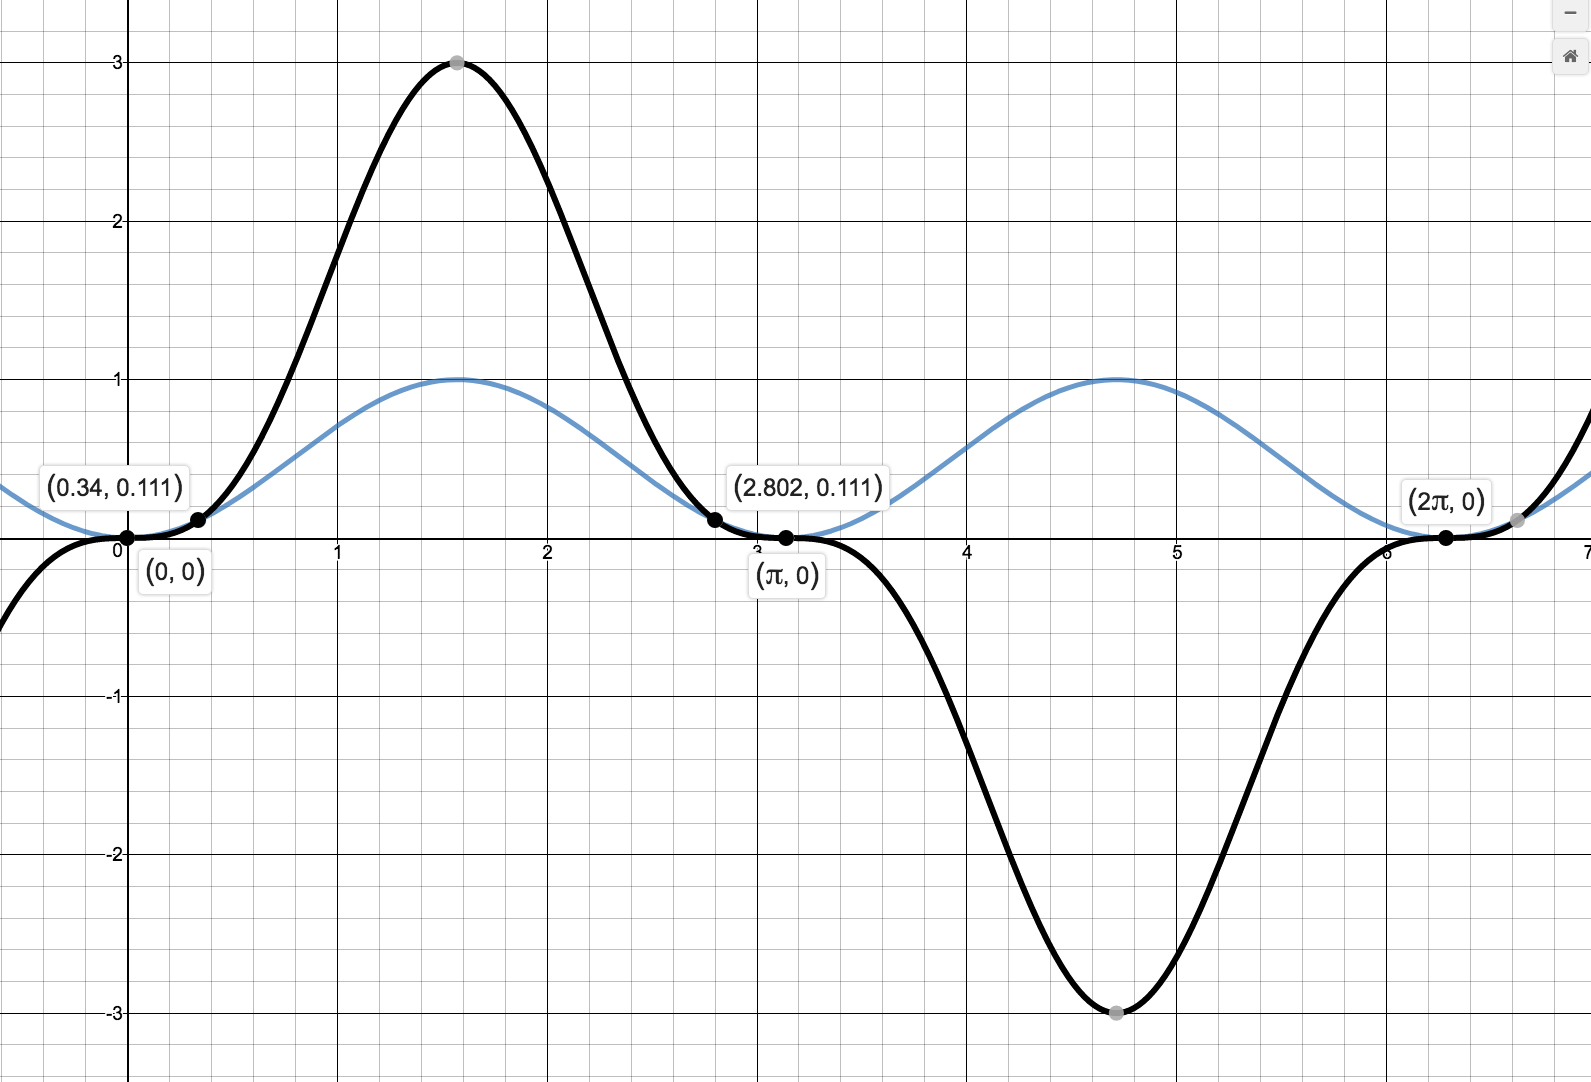
\includegraphics[height=2.25in]{./TrigonometricEquationsandInequalitiesGraphics/TrigEquIneq07.jpg} 

{\boldmath $y = 3(\sin(\theta))^3$} and  $y = (\sin(\theta))^2$


\end{center} 

\item We see immediately in the equation $\sec^{2}(\theta) = \tan(\theta) + 3$ that there are two different circular functions present, so we look for an identity to express both sides in terms of the same function.  

\smallskip

We use the Pythagorean Identity $\sec^{2}(\theta) = 1 + \tan^{2}(\theta)$ to exchange $\sec^{2}(\theta)$  for tangents.  What results is a `quadratic in disguise:'\footnote{See Section \ref{AppQuadEqus} for a review of this concept.}

\[ \begin{array}{rclr}

\sec^{2}(\theta) &  = & \tan(\theta) + 3 & \\
1 + \tan^{2}(\theta) & = & \tan(\theta) + 3& \text{(Since $\sec^{2}(\theta) = 1 + \tan^{2}(\theta)$.)} \\
\tan^{2}(\theta) - \tan(\theta) -2 & = & 0 & \\
u^2 - u - 2 & = & 0 & \text{Let $u = \tan(\theta)$.} \\
(u + 1)(u - 2) & = & 0 & \\ \end{array} \]

This gives $u = -1$ or $u = 2$.  Since $u = \tan(\theta)$, we have $\tan(\theta) = -1$ or $\tan(\theta) = 2$. 

\smallskip

From $\tan(\theta) = -1$, we get $\theta = -\frac{\pi}{4} + \pi k$ for integers $k$.  To solve $\tan(\theta) = 2$, we employ the arctangent function and get $\theta = \arctan(2) + \pi k$ for integers $k$.  

\smallskip

From the first set of solutions, we get $\theta = \frac{3\pi}{4}$ and $\theta = \frac{7\pi}{4}$ as our answers which lie in $[0,2\pi)$.  

\smallskip

Using the same sort of argument we saw in Example \ref{TrigEqnEx1},   we get  $\theta=\arctan(2) \approx 1.107$ and $\theta = \pi + \arctan(2) \approx 4.249$ as answers from our second set of solutions which lie in $[0,2\pi)$.  

\smallskip

We verify our solutions below graphically.  

\begin{center}

 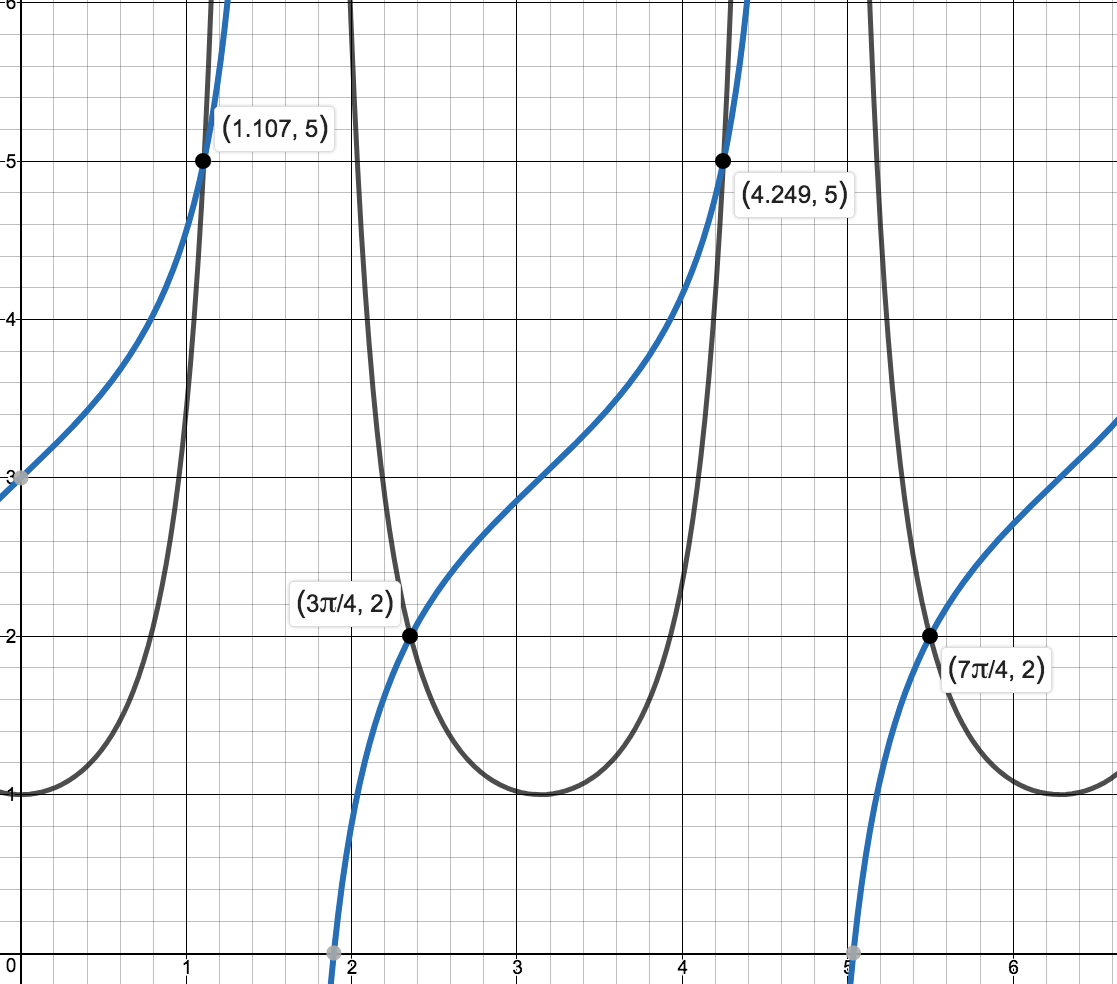
\includegraphics[height=2.25in]{./TrigonometricEquationsandInequalitiesGraphics/TrigEquIneq08.jpg} \\

{ \boldmath  $y =(\sec(\theta))^2$} and $y = \tan(\theta) + 3$  
 
\end{center}

\item  The good news is that in the equation $\cos(2t) = 3\cos(t) - 2$, we have the same circular function, cosine,  throughout.  The bad news is that we have different arguments, $2t$ and $t$.  

\smallskip

Using the double angle identity $\cos(2t) = 2\cos^{2}(t) - 1$ results in another quadratic in disguise:'

\[ \begin{array}{rclr}

\cos(2t) & = & 3\cos(t) - 2 & \\
2\cos^{2}(t) -1 & = & 3\cos(t) -2 & \text{(Since $\cos(2t) = 2\cos^{2}(t) -1$.)} \\
2\cos^{2}(t) - 3\cos(t) +1 & = & 0 & \\
2 u^2 - 3 u + 1 & = & 0 & \text{Let $u = \cos(t)$.}\\
(2u - 1)(u - 1) & = & 0 & \\ \end{array} \]

We get $u = \frac{1}{2}$ or $u = 1$, so   $\cos(t) = \frac{1}{2}$ or $\cos(t) = 1$. Solving  $\cos(t) = \frac{1}{2}$, we get $t = \frac{\pi}{3} + 2\pi k$ or $t = \frac{5\pi}{3} + 2\pi k$ for integers $k$.  From $\cos(t) = 1$, we get $t = 2\pi k$ for integers $k$.  

\smallskip

The answers which lie in $[0,2\pi)$ are $t =0$,  $\frac{\pi}{3}$, and $\frac{5\pi}{3}$.  Graphing $y = \cos(2t)$ and $y = 3\cos(t) - 2$, we find that the curves intersect in three places on $[0,2\pi)$ and confirm our results.

\begin{center}

 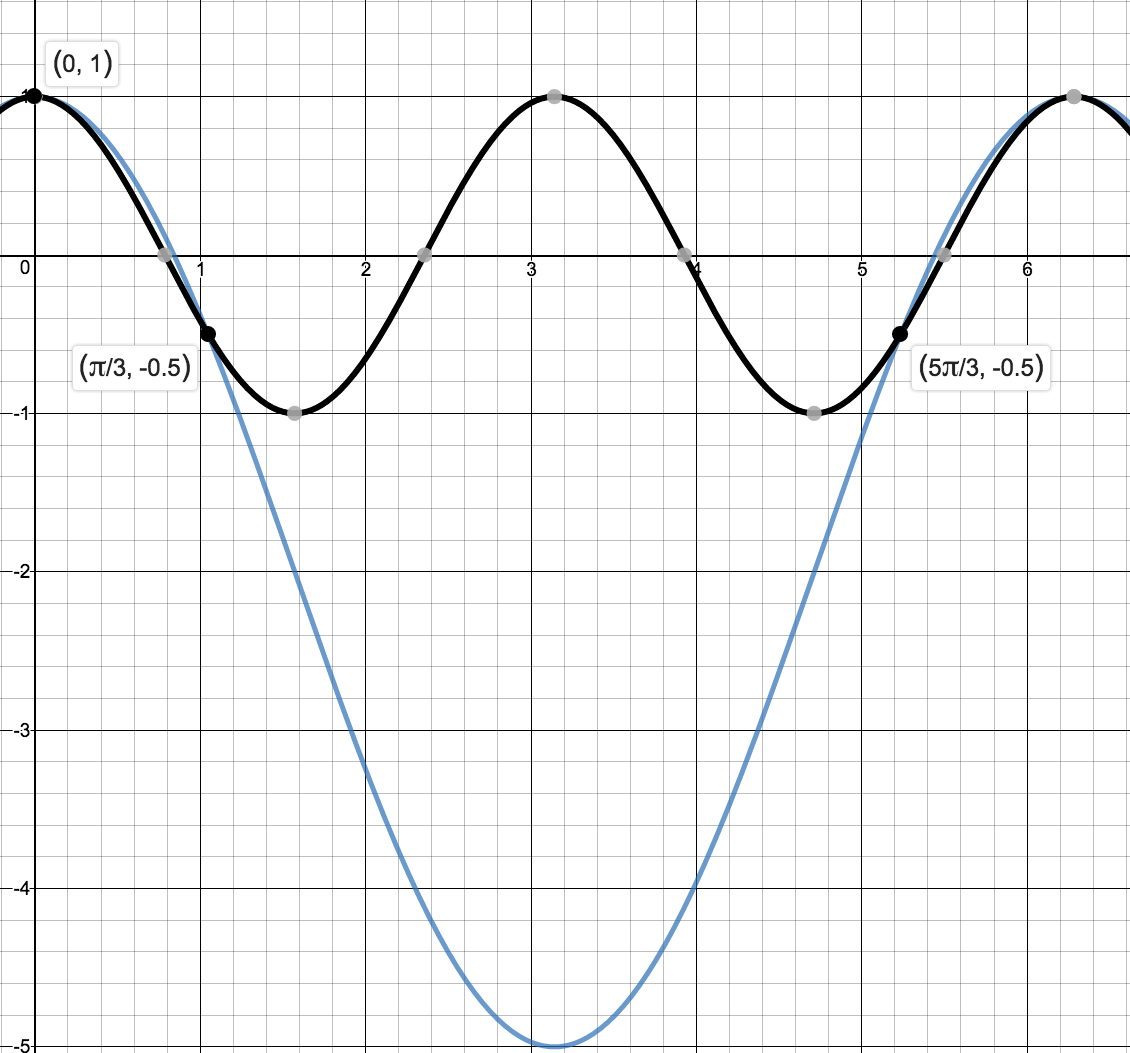
\includegraphics[height=2.25in]{./TrigonometricEquationsandInequalitiesGraphics/TrigEquIneq09.jpg}

{ \boldmath  $y =\cos(2t)$} and $y = 3 \cos(t)  - 2$  
 
\end{center}



\item  To solve $\cos(3t) = 2- \cos(t)$, we take a cue from the previous problem and look for an identity to rewrite $\cos(3t)$ in terms of $\cos(t)$.

\smallskip

  From Example \ref{doubleangleex}, number \ref{cosinepolynomial}, we know that $\cos(3t) = 4\cos^{3}(t) - 3\cos(t)$.  This transforms the equation into a polynomial in terms of $\cos(t)$.


\[ \begin{array}{rclr}

\cos(3t) & = &2- \cos(t) & \\
4\cos^{3}(t) - 3\cos(t) & = & 2- \cos(t) & \\
2\cos^{3}(t) - 2\cos(t) -2  & = & 0 & \\
4 u^3 - 2 u -2  & = & 0 & \text{Let $u = \cos(t)$.} \\ \end{array} \]

Using what we know from Chapter \ref{PolynomialFunctions}, we factor $4u^3-2u-2$ as $(u-1)\left(4u^2+4u+2\right)$ and set each factor equal to $0$.  

\smallskip

We get either $u-1 = 0$ or  $4u^2+2u+2=0$, and since the discriminant of the latter is negative, the only real solution to $4u^3-2u-2=0$ is $u = 1$.  


\smallskip

Since $u = \cos(t)$, we get $\cos(t) = 1$, so $t = 2\pi k$ for integers $k$.  The only solution which lies in $[0,2\pi)$ is $t = 0$.  Our graph below confirms this.

\begin{center}

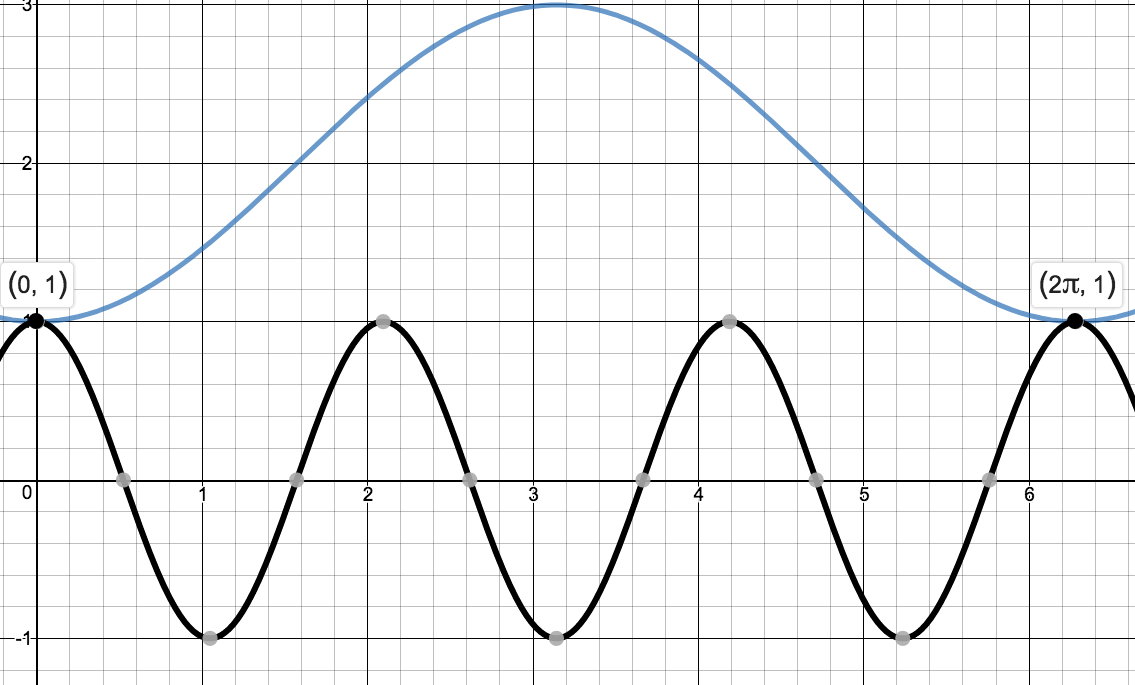
\includegraphics[height=2.25in]{./TrigonometricEquationsandInequalitiesGraphics/TrigEquIneq10.jpg} 

{\boldmath $y = \cos(3t)$} and  $y = 2- \cos(t)$
\end{center}


\item  While we could approach solving the equation $\cos(3x) = \cos(5x)$ in the same manner as we did the previous two problems, we choose instead to showcase the utility of the Sum to Product Identities.\footnote{We invite the reader to try the `polynomial approach' used in the previous problem to see what difficulties are encountered.}

\smallskip

From $\cos(3x) = \cos(5x)$, we get $\cos(5x) - \cos(3x) = 0$, and it is the presence of $0$ on the right hand side that indicates a switch to a product would be a good move.\footnote{Since a \textit{product} equalling zero means, necessarily, one or both \textit{factors} is $0$.  See page \ref{propertiesofzero}.}

\smallskip

 Using Theorem \ref{sumtoproduct}, we rewrite $\cos(5x) - \cos(3x)$  as $- 2 \sin\left( \frac{5x + 3x}{2}\right)\sin\left( \frac{5x - 3x}{2}\right) = -2 \sin(4x)\sin(x)$.  Hence, our original equation $\cos(3x) = \cos(5x)$ is equivalent to $-2 \sin(4x) \sin(x) = 0$.  
 
 \smallskip
 
From $-2 \sin(4x) \sin(x) = 0$, we get either  $\sin(4x) = 0$ or $\sin(x)$ = 0. Solving $\sin(4x) = 0$ gives $x = \frac{\pi}{4} k$ for integers $k$, and the solution to $\sin(x) = 0$ is $x = \pi k$ for integers $k$.  

\smallskip

The second set of solutions is contained in the first set of solutions,\footnote{As always, when in doubt, write it out!} so our final solution to $\cos(5x) = \cos(3x)$ is $x = \frac{\pi}{4} k$ for integers $k$.  

\smallskip

There are eight of these answers which lie in $[0,2\pi)$:  $x = 0$, $\frac{\pi}{4}$, $\frac{\pi}{2}$, $\frac{3\pi}{4}$, $\pi$, $\frac{5\pi}{4}$, $\frac{3\pi}{2}$ and $\frac{7\pi}{4}$.  Our plot of the graphs of $y = \cos(3x)$ and $y = \cos(5x)$ below (after some careful zooming) bears this out. 

\begin{center}

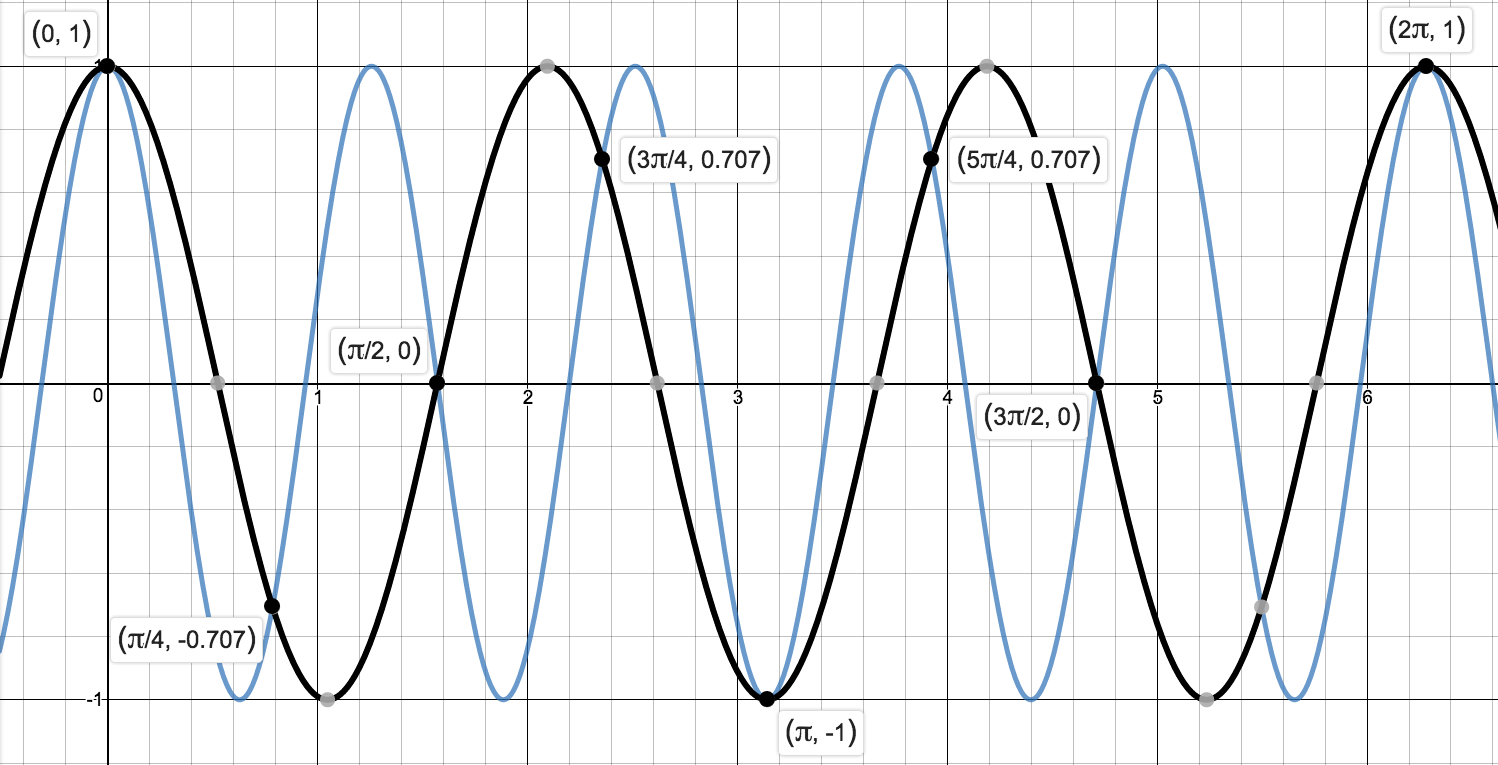
\includegraphics[height=2.25in]{./TrigonometricEquationsandInequalitiesGraphics/TrigEquIneq11.jpg} 

{\boldmath $y = \cos(3x)$} and  $y = cos(5x)$

\end{center}

\item  In the equation   $\sin(2x) =\sqrt{3} \cos(x)$, we not only  have different circular functions involved,  but we also have different arguments to contend with.  

\smallskip

Using the double angle identity $\sin(2x) = 2 \sin(x) \cos(x)$ makes all of the arguments the same and we proceed to gather all of the nonzero terms on one side of the equation and factor.

\[ \begin{array}{rclr}

\sin(2x) & = & \sqrt{3} \cos(x) & \\
2 \sin(x) \cos(x) & = & \sqrt{3} \cos(x)  & \text{(Since $\sin(2x) = 2\sin(x) \cos(x)$.)} \\
2\sin(x) \cos(x) - \sqrt{3} \cos(x) & = & 0 & \\
\cos(x) (2 \sin(x) - \sqrt{3}) & = & 0 & \\ \end{array} \]

We get $\cos(x) = 0$ or $\sin(x) = \frac{\sqrt{3}}{2}$. From $\cos(x) = 0$, we obtain $x = \frac{\pi}{2} + \pi k$ for integers $k$. From $\sin(x) = \frac{\sqrt{3}}{2}$, we get $x = \frac{\pi}{3} + 2\pi k$ or $x = \frac{2\pi}{3} + 2\pi k$ for integers $k$.  

\smallskip

The answers which lie in $[0,2\pi)$ are $x = \frac{\pi}{2}$, $\frac{3\pi}{2}$, $\frac{\pi}{3}$ and $\frac{2\pi}{3}$, as verified graphically below.

\begin{center}

 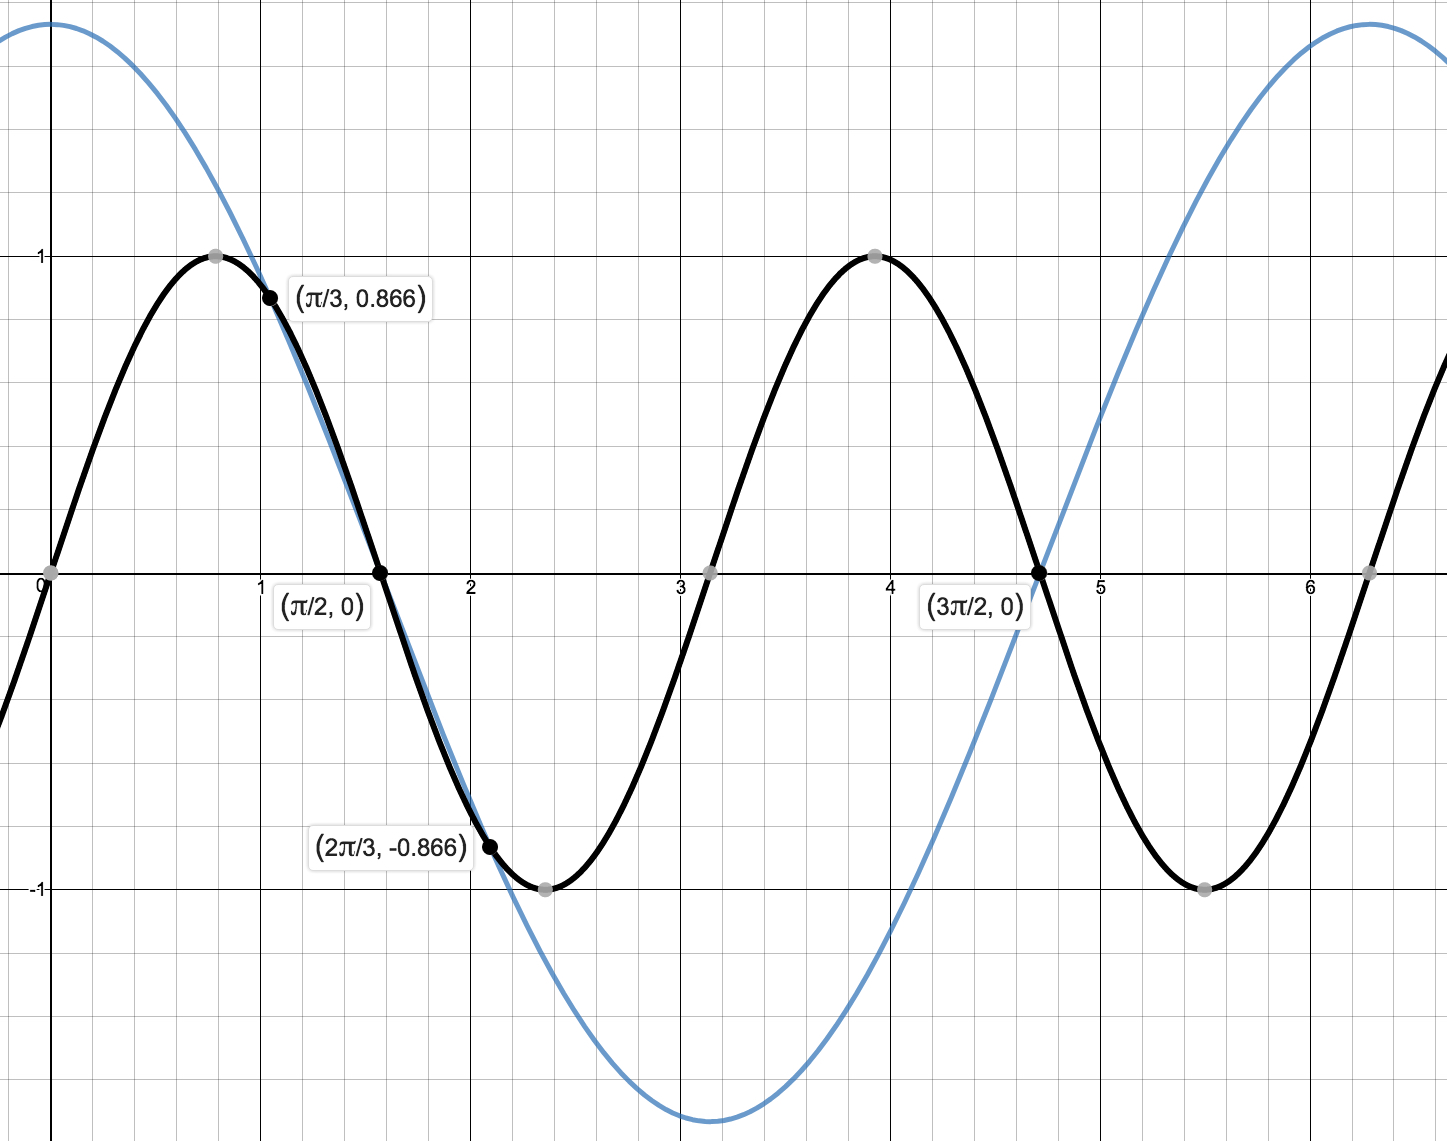
\includegraphics[height=2.25in]{./TrigonometricEquationsandInequalitiesGraphics/TrigEquIneq12.jpg} 

{\boldmath $y = \sin(2x)$} and  $y = \sqrt{3} \cos(x)$  
 
\end{center}

\item Unlike the previous problem, there seems to be no quick way to get the circular functions or their arguments to match in the equation $\sin(x)\cos\left(\frac{x}{2}\right) + \cos(x)\sin\left(\frac{x}{2}\right) = 1$. 

\smallskip

 If we stare at it long enough, however,  we realize that the left hand side is the expanded form of the sum formula for $\sin\left(x + \frac{x}{2}\right)$.  Hence, our original equation is equivalent to  $\sin\left(\frac{3}{2} x\right) = 1$.  
 
 \smallskip
 
 Solving, we find $x = \frac{\pi}{3} + \frac{4\pi}{3} k$ for integers $k$.  Two of these solutions lie in $[0,2\pi)$: $x = \frac{\pi}{3}$ and $x = \frac{5\pi}{3}$. Graphing $y = \sin(x)\cos\left(\frac{x}{2}\right) + \cos(x)\sin\left(\frac{x}{2}\right)$ and $y = 1$ validates our solutions.
 
 
\begin{center}

 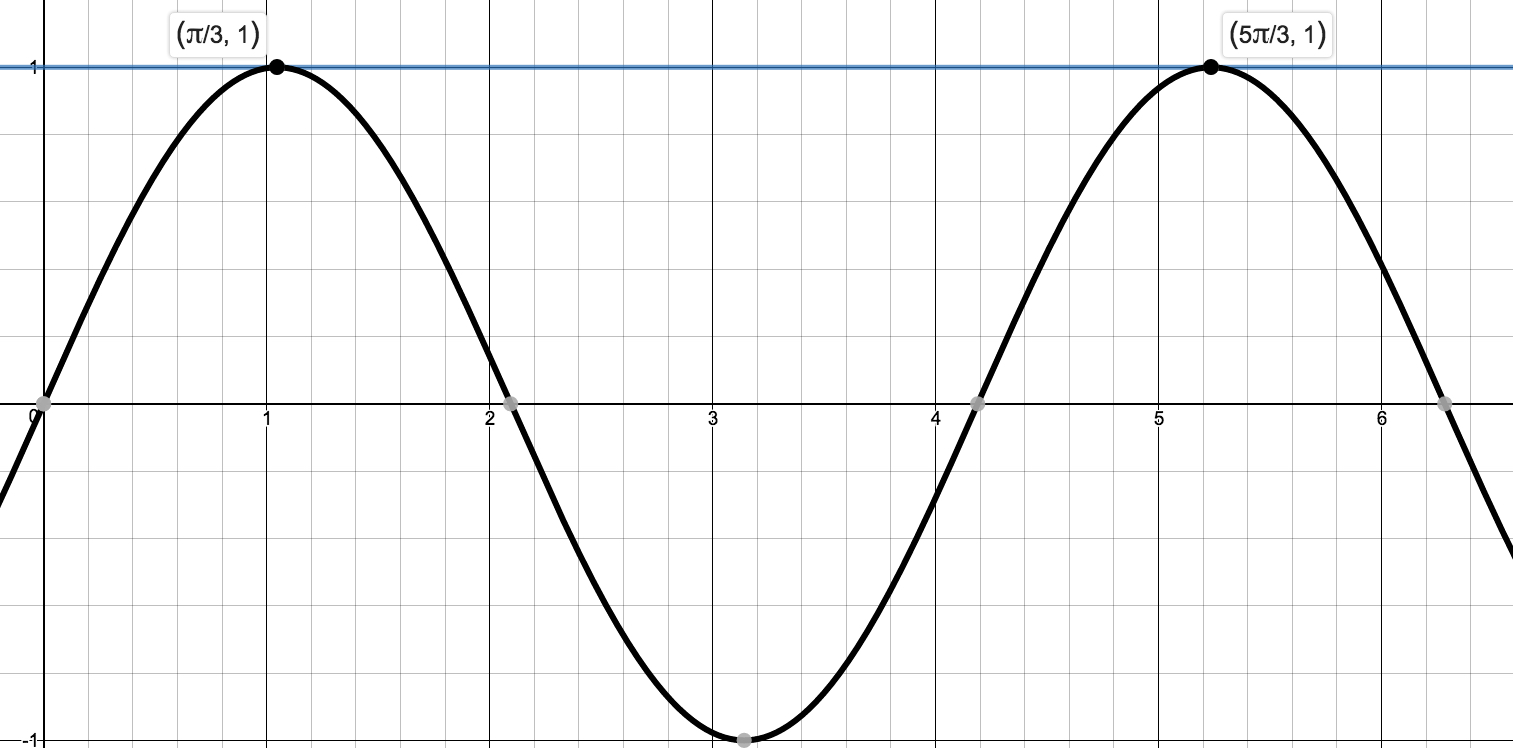
\includegraphics[height=2.25in]{./TrigonometricEquationsandInequalitiesGraphics/TrigEquIneq13.jpg} 

{\boldmath $y = \sin(x)\cos\left(\frac{x}{2}\right) + \cos(x)\sin\left(\frac{x}{2}\right)$} and $y = 1$
 
\end{center}


\item  With the absence of double angles or squares, there doesn't seem to be much we can do with the equation $\cos(x) - \sqrt{3} \sin(x) = 2$.  

\smallskip

However, since the frequencies of the sine and cosine terms are the same, we can rewrite the left hand side of this equation as a sinusoid.

\smallskip

 To fit $f(x) = \cos(x) - \sqrt{3} \sin(x)$ to the form $A\sin(\omega t + \phi) + B$, we use what we learned in Example \ref{expandedsinusoidex1} and find $A = 2$, $B = 0$, $\omega = 1$ and $\phi = \frac{5\pi}{6}$.   
 
 \smallskip
 
 Hence, we can rewrite the equation  $\cos(x) - \sqrt{3} \sin(x) = 2$  as $2 \sin\left(x + \frac{5\pi}{6}\right) = 2$, or $\sin\left(x + \frac{5\pi}{6}\right) = 1$.   Solving, we get $x  = - \frac{\pi}{3} + 2\pi k$ for integers $k$.
 
 \smallskip
 
Only one of our solutions, $x = \frac{5\pi}{3}$, which corresponds to $k=1$, lies in $[0,2\pi)$.  Geometrically, we see that $y = \cos(x) - \sqrt{3} \sin(x)$ and $y = 2$ intersect just once, supporting our answer.

\begin{center}

 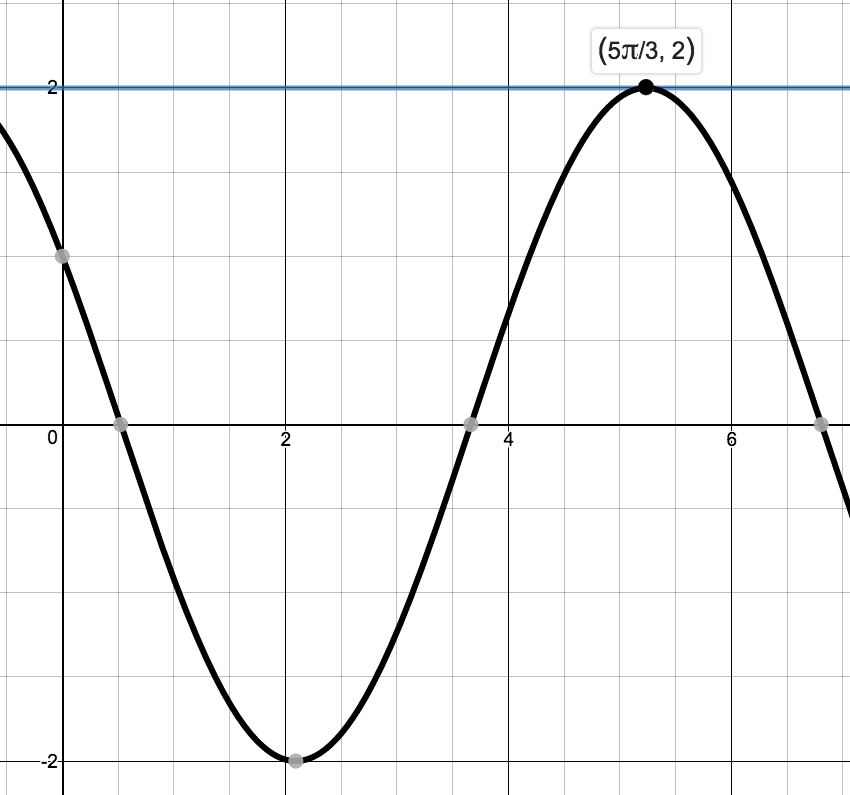
\includegraphics[height=2.25in]{./TrigonometricEquationsandInequalitiesGraphics/TrigEquIneq14.jpg} 

{\boldmath  $y = \cos(x) - \sqrt{3} \sin(x)$} and  $y = 2$

\end{center}

An alternative way to solve this problem is to \textit{introduce} squares in order to exchange sines and cosines using a Pythagorean Identity. 

\smallskip

 From  $\cos(x) - \sqrt{3} \sin(x) = 2$ we get $\sqrt{3} \sin(x) = \cos(x) - 2$ so that $\left(\sqrt{3} \sin(x)\right)^2 = \left(\cos(x) - 2\right)^2$.  Simplifying, we get: $3 \sin^{2}(x) = \cos^{2}(x) - 4 \cos(x) + 4$.
 
 \smallskip
 
 Substituting $\sin^{2}(x) = 1 - \cos^{2}(x)$, we get $3(1 - \cos^{2}(x)) = \cos^{2}(x) - 4\cos(x) + 4$ which results in the quadratic equation: $4 \cos^{2}(x) - 4 \cos(x) +1 = 0$.  
 
 \smallskip
 
 Letting $u = \cos(x)$, we get $4u^2 - 4u + 1 = 0$ or $(2u - 1)^2 = 0$.  We get $u = \cos(x) = \frac{1}{2}$.  Solving $\cos(x) = \frac{1}{2}$ gives $x = \frac{\pi}{3} + 2\pi k$ as well as $x = \frac{5\pi}{3} + 2\pi k$ for integers, $k$.  
 
 \smallskip
 
 Of these two families, only  solutions of the form $x = \frac{5\pi}{3} + 2\pi k$ checks in our original equation.\footnote{We've seen how squaring both sides can lead to extraneous solutions in Section \ref{AppRadEqus} and Chapter \ref{RootRadicalPowerFunctions}.  Here, squaring both sides admits an entire \textit{family} of extraneous solutions.}  We leave it the reader to verify this representation of solutions to $\cos(x) - \sqrt{3} \sin(x) = 2$ is equivalent to the one we found previously. \qed

\end{enumerate}

\end{ex}
 
We repeat here the advice given when solving systems of nonlinear equations in section \ref{NonLinearEquations} --  when it comes to solving equations involving the circular functions, it helps to just try something.  

\smallskip

Next, we focus on solving inequalities involving the circular functions.  Since these functions are continuous on their domains, we may use the sign diagram technique we've used in the past to solve the inequalities.\footnote{See pages \pageref{firstsigndiagram}, \pageref{rationalsigndiagram},  \pageref{algebraicsigndiagram}, as well as Examples \ref{expineq} and \ref{logineq} for a review of this technique, as needed.}

\begin{ex}  \label{TrigIneqEx1} Solve the following inequalities on $[0,2\pi)$.  Express your answers using interval notation and verify your answers graphically.

\begin{multicols}{3}

\begin{enumerate}

\item  $2\sin(t) \leq 1$

\item  $\sin(2x) > \cos(x)$

\item  $\tan(x) \geq 3$

\end{enumerate}

\end{multicols}

\newpage

{\bf Solution.}

\begin{enumerate}

\item  We begin solving $2\sin(t) \leq 1$ by collecting all of the terms on one side of the equation and zero on the other to get $2\sin(t) - 1 \leq 0$.  

\smallskip

Next, we let $f(t) = 2\sin(t) - 1$ and note that our original inequality is equivalent to solving $f(t) \leq 0$. We now look to see where, if ever, $f$ is undefined and where $f(t) = 0$.  

\smallskip

Since the domain of $f$ is all real numbers, we can immediately set  about finding the zeros of $f$.  Solving $f(t) = 0$, we have $2\sin(t) - 1=0$ or $\sin(t) = \frac{1}{2}$.  The solutions here are $t = \frac{\pi}{6} + 2\pi k$ and $t = \frac{5\pi}{6} + 2\pi k$ for integers $k$.  Since we are restricting our attention to $[0,2\pi)$, only $t = \frac{\pi}{6}$ and $t = \frac{5\pi}{6}$ are of concern.

\smallskip

 Next, we choose test values in $[0,2\pi)$ other than the zeros and determine if $f$ is positive or negative there.  For $t = 0$ we have $f(0) = -1$, for $t = \frac{\pi}{2}$ we get $f\left(\frac{\pi}{2}\right) = 1$ and for $t = \pi$ we get $f(\pi) = -1$.  
 
 \smallskip
 
 Since our original inequality is equivalent to $f(t) \leq 0$, we are looking for where the function is negative $(-)$ or $0$, and we get the intervals $\left[0, \frac{\pi}{6}\right] \cup \left[\frac{5\pi}{6}, 2\pi \right)$.  We can confirm our answer graphically by seeing where the graph of $y = 2\sin(t)$ crosses or is below the graph of $y = 1$. 

\begin{center}

\begin{mfpic}[10]{-6}{6}{-2}{2}
\polyline{(-6,0),(6,0)}
\xmarks{-6,-2,2,6}
\tiny
\tlpointsep{6pt}
\normalsize
\tlabel[cc](-6,-1){$0$}
\tlabel[cc](-4,1){$(-)$}
\tlabel[cc](-2,-1){$\frac{\pi}{6}$}
\tlabel[cc](-2,1){0}
\tlabel[cc](0,1){$(+)$}
\tlabel[cc](2,-1){$\frac{5\pi}{6}$}
\tlabel[cc](2,1){$0$}
\tlabel[cc](4,1){$(-)$}
\tlabel[cc](6,-1){$2\pi$}
\end{mfpic} 



 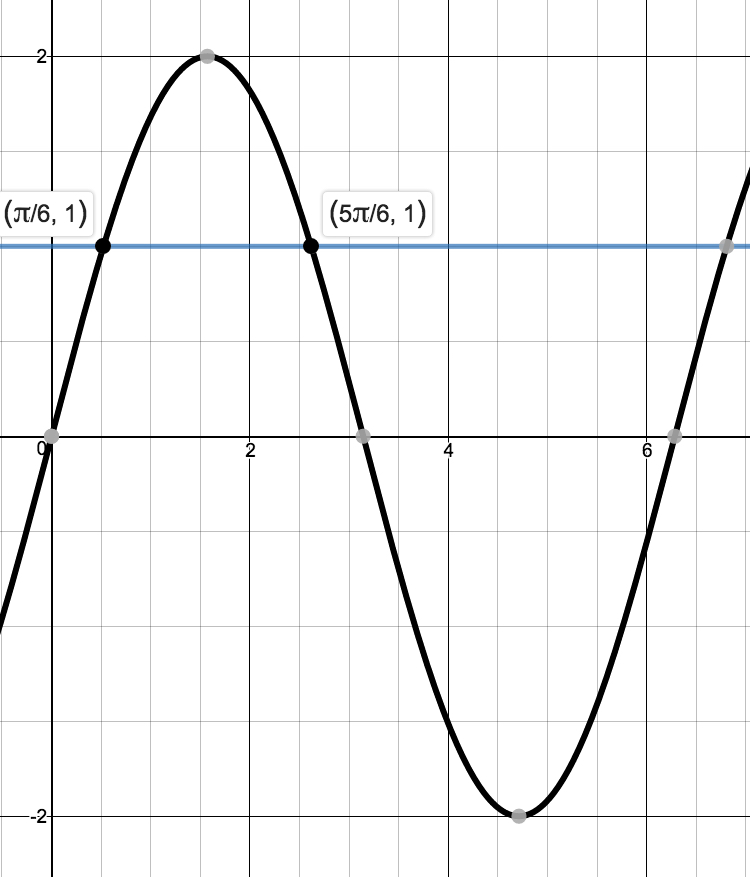
\includegraphics[height=2.5in]{./TrigonometricEquationsandInequalitiesGraphics/TrigEquIneq15.jpg}
 
 {\boldmath $y = 2\sin(t)$} and $y = 1$ 



\end{center}


\item  We first rewrite  $\sin(2x) > \cos(x)$   as $\sin(2x) - \cos(x) > 0$ and let $f(x) = \sin(2x) - \cos(x)$.  

\smallskip

Our original inequality is thus equivalent to $f(x) > 0$.  The domain of $f$ is all real numbers, so we can advance to finding the zeros of $f$. 

\smallskip

Setting $f(x) = 0$ yields $\sin(2x) - \cos(x) = 0$, which, by way of the double angle identity for sine, becomes $2\sin(x)\cos(x) - \cos(x) = 0$ or $\cos(x) (2\sin(x) - 1) = 0$.  

\smallskip

From $\cos(x) = 0$, we get $x = \frac{\pi}{2} + \pi k$ for integers $k$ of which only $x = \frac{\pi}{2}$ and $x = \frac{3\pi}{2}$ lie in $[0,2\pi)$.  

\smallskip

For $2\sin(x) - 1 = 0$, we get $\sin(x) = \frac{1}{2}$ which gives $x = \frac{\pi}{6} + 2\pi k$ or $x = \frac{5\pi}{6} + 2\pi k$ for integers $k$.  Of those, only $x = \frac{\pi}{6}$ and $x = \frac{5\pi}{6}$ lie in $[0,2\pi)$.  

\smallskip

Choosing test values, we get: for  $x =0$ we find $f(0) = -1$; when $x = \frac{\pi}{4}$ we get $f\left(\frac{\pi}{4}\right) =1 - \frac{\sqrt{2}}{2} = \frac{2 - \sqrt{2}}{2}$;  for $x = \frac{3\pi}{4}$ we get $f\left(\frac{3\pi}{4}\right) =-1 + \frac{\sqrt{2}}{2} =  \frac{\sqrt{2} - 2}{2}$;  when $x=\pi$ we have $f(\pi) = 1$, and lastly, for $x = \frac{7\pi}{4}$ we get $f\left(\frac{7\pi}{4}\right) = -1 - \frac{\sqrt{2}}{2} =  \frac{-2 - \sqrt{2}}{2}$.  

\smallskip

We see $f(x) > 0$ on $\left(\frac{\pi}{6}, \frac{\pi}{2}\right) \cup \left(\frac{5\pi}{6}, \frac{3\pi}{2}\right)$, so this is our answer.  Geometrically, we see the graph of $y = \sin(2x)$ is indeed above the graph of $y = \cos(x)$ on those intervals. 

\begin{center}


\begin{mfpic}[10]{-10}{10}{-2}{2}
\polyline{(-10,0),(10,0)}
\xmarks{-10,-6,-2,2,6,10}
\tiny
\tlpointsep{6pt}
\normalsize
\tlabel[cc](-10,-1){$0$}
\tlabel[cc](-8,1){$(-)$}
\tlabel[cc](-6,-1){$\frac{\pi}{6}$}
\tlabel[cc](-6,1){0}
\tlabel[cc](-4,1){$(+)$}
\tlabel[cc](-2,-1){$\frac{\pi}{2}$}
\tlabel[cc](-2,1){0}
\tlabel[cc](0,1){$(-)$}
\tlabel[cc](2,-1){$\frac{5\pi}{6}$}
\tlabel[cc](2,1){0}
\tlabel[cc](4,1){$(+)$}
\tlabel[cc](6,-1){$\frac{3\pi}{2}$}
\tlabel[cc](6,1){0}
\tlabel[cc](8,1){$(-)$}
\tlabel[cc](10,-1){$2\pi$}
\end{mfpic} 

 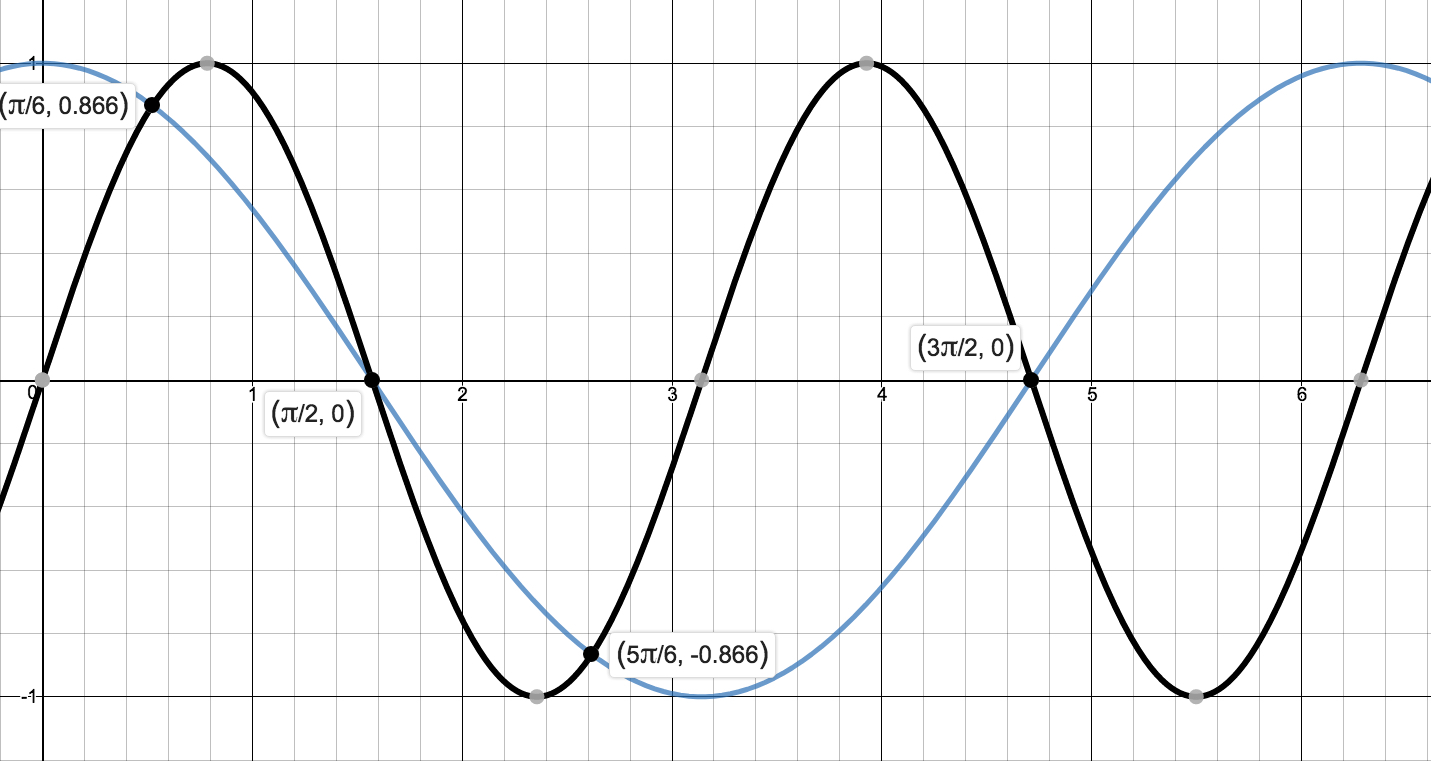
\includegraphics[height=2.5in]{./TrigonometricEquationsandInequalitiesGraphics/TrigEquIneq16.jpg}

 {\boldmath $y = \sin(2x)$} and  $y = \cos(x)$ 

\end{center}

\item  Proceeding as above, we rewrite  $\tan(x) \geq 3$ as $\tan(x) - 3 \geq 0$ and let $f(x) = \tan(x) - 3$.  

\smallskip

We note that on $[0,2\pi)$, $f$ is undefined at $x =\frac{\pi}{2}$ and $\frac{3\pi}{2}$, so those values will need the usual disclaimer on the sign diagram.\footnote{See page \pageref{rationalsigndiagram} for a discussion of the non-standard character known as the interrobang.}  

\smallskip

Moving along to zeros, solving $f(x) = \tan(x) - 3 = 0$ requires the arctangent function.  We find $x = \arctan(3) + \pi k$ for integers $k$ and of these, only $x = \arctan(3)$ and $x = \arctan(3) + \pi$ lie in $[0,2\pi)$.  Since $3 > 0$, we know $0 < \arctan(3) < \frac{\pi}{2}$ which allows us to position these zeros correctly on the sign diagram. 

\smallskip

To choose test values, we begin with $x=0$ and find $f(0) = -3$. Finding a convenient test value in the interval $\left(\arctan(3), \frac{\pi}{2}\right)$ is a bit more challenging.  Since the arctangent function is increasing and is bounded above by $\frac{\pi}{2}$,  the number $x = \arctan(117)$ is guaranteed\footnote{We could have chosen any value $\arctan(t)$ where $t > 3$.} to lie between  $\arctan(3)$ and $\frac{\pi}{2}$.  We see that $f(\arctan(117)) = \tan(\arctan(117)) - 3 = 114$.  

\smallskip

For our next test value, we take $x = \pi$ and find $f(\pi) = -3$, which brings us to finding a test value in the interval $\left(\arctan(3) + \pi, \frac{3\pi}{2} \right)$.

\smallskip

From $\arctan(3) < \arctan(117) < \frac{\pi}{2}$ we get $\arctan(3) + \pi < \arctan(117) + \pi < \frac{3\pi}{2}$ by adding $\pi$ through the inequality.  We find $f(\arctan(117)+\pi) = \tan(\arctan(117) + \pi) -3 = \tan(\arctan(117)) - 3 = 114$.  

\smallskip

For our last test value, we choose $x = \frac{7\pi}{4}$ and find $f\left(\frac{7\pi}{4}\right) = -4$.  

\smallskip

Since we want $f(x) \geq 0$, we see that our answer is $\left[ \arctan(3), \frac{\pi}{2}\right) \cup  \left[\arctan(3)+\pi, \frac{3\pi}{2}\right)$.  Using the graphs of $y = \tan(x)$ and $y = 3$, we see when the graph of the former is above (or meets) the graph of the latter. (Note, $\arctan(3) \approx 1.249$ and $\arctan(3) + \pi \approx 4.391$.)

\begin{center}

\begin{mfpic}[10]{-10}{10}{-2}{2}
\polyline{(-10,0),(10,0)}
\xmarks{-10,-6,-2,2,6,10}
\tiny
\tlpointsep{6pt}
\normalsize
\tlabel[cc](-10,-1){$0$}
\tlabel[cc](-8,1){$(-)$}
\tlabel[cc](-6,-1){\tiny $\arctan(3)$}
\tlabel[cc](-6,1){0}
\tlabel[cc](-4,1){$(+)$}
\tlabel[cc](-2,-1){$\frac{\pi}{2}$}
\tlabel[cc](-2,1){\textinterrobang}
\tlabel[cc](0,1){$(-)$}
\tlabel[cc](2,-1){\tiny $(\arctan(3)+\pi)$}
\tlabel[cc](2,1){0}
\tlabel[cc](4,1){$(+)$}
\tlabel[cc](6,-1){$\frac{3\pi}{2}$}
\tlabel[cc](6,1){\textinterrobang}
\tlabel[cc](8,1){$(-)$}
\tlabel[cc](10,-1){$2\pi$}
\end{mfpic} 

 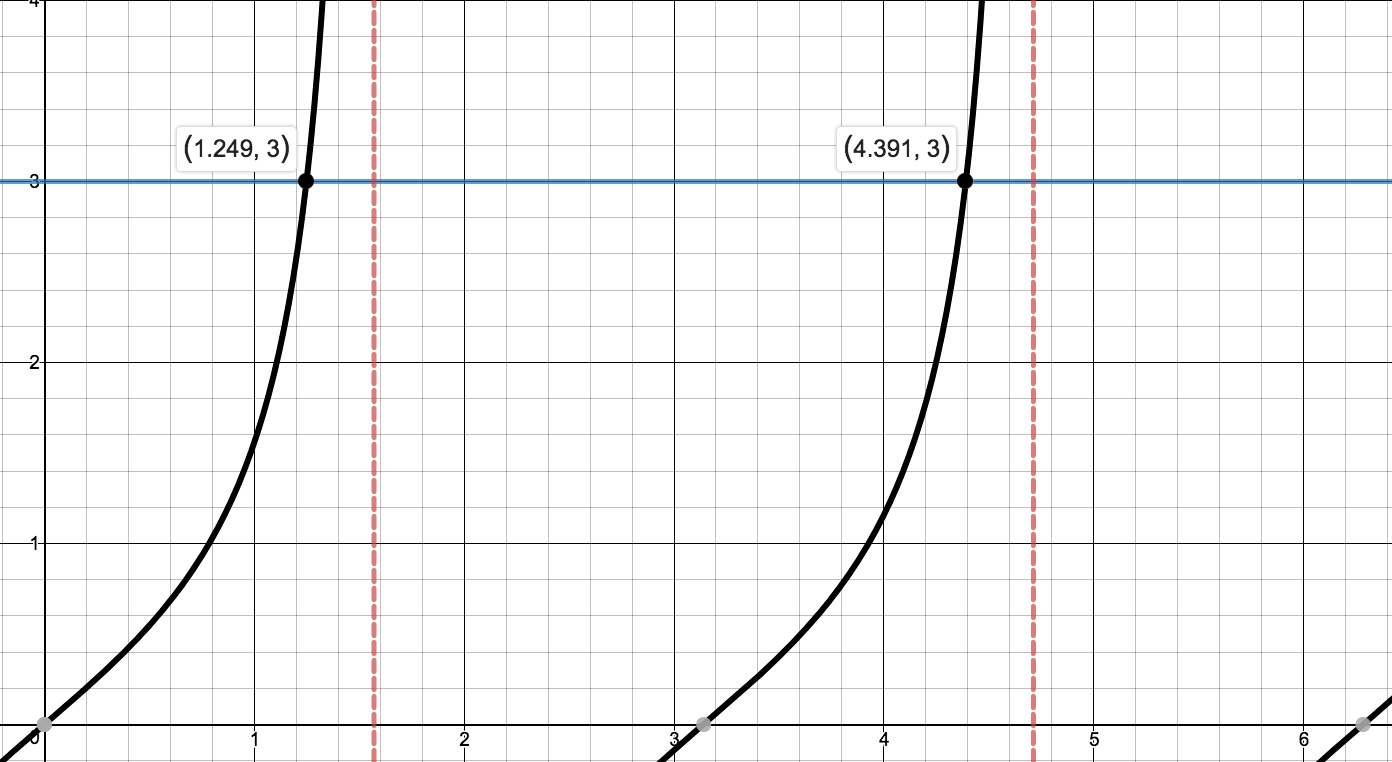
\includegraphics[height=2.5in]{./TrigonometricEquationsandInequalitiesGraphics/TrigEquIneq17.jpg} 
 
 {\boldmath $y = \tan(x)$} and $y =3$ 

\end{center}


\vspace{-.25in} \qed

\end{enumerate}


\end{ex}


Our next example puts solving equations and inequalities to good use -- finding domains of functions.


\begin{ex}  \label{TrigDomainEx1} Express the domain of the following functions using extended interval notation.\footnote{See Section \ref{extendedinterval} for details about this notation.}

\begin{multicols}{3}

\begin{enumerate}

\item  $f(x) = \csc\left(2x + \frac{\pi}{3}\right)$

\item  $f(t) = \dfrac{\sin(t)}{2\cos(t) - 1}$

\item  $f(x) = \sqrt{1 - \cot(x)}$

\end{enumerate}

\end{multicols}

\newpage

{\bf Solution.}

\begin{enumerate}

\item  To find the domain of $f(x) = \csc\left(2x + \frac{\pi}{3}\right)$, we rewrite $f$ in terms of sine as $f(x) = \frac{1}{\sin\left(2x + \frac{\pi}{3}\right)}$.  Since the sine function is defined everywhere, our only concern comes from zeros in the denominator.  

\smallskip

Solving $\sin\left(2x + \frac{\pi}{3}\right) = 0$, we get $x = -\frac{\pi}{6} + \frac{\pi}{2} k$ for integers $k$.  In set-builder notation, our domain is  $\left\{ x \, | \, x  \neq  -\frac{\pi}{6} + \frac{\pi}{2} k \, \text{for integers $k$} \right\}$.  To help visualize the domain,  we follow the old mantra `When in doubt, write it out!' We get $\left\{ x \, | \, x  \neq  -\frac{\pi}{6}, \frac{2\pi}{6}, -\frac{4\pi}{6}, \frac{5\pi}{6}, -\frac{7\pi}{6}, \frac{8\pi}{6}, \ldots \right\}$, where we have kept the denominators $6$ throughout to help see the pattern.  Graphing the situation on a number line, we have

\begin{center}

\begin{mfpic}[15]{-6}{6}{-1}{2}
\arrow \reverse \arrow \polyline{(-6,0), (6,0)}
\xmarks{-5,-3,-1,1,3,5}
\tlpointsep{5pt}
\axislabels {x}{{\small $-\frac{7\pi}{6} \hspace{7pt}$} -5,{\small $-\frac{4\pi}{6} \hspace{7pt}$} -3, {\small $-\frac{\pi}{6} \hspace{7pt}$} -1,{\small $\frac{2\pi}{6}$} 1,{\small $\frac{5\pi}{6}$} 3,  {\small $\frac{8\pi}{6}$} 5}

\penwd{1.5}
\arrow \reverse \arrow \polyline{(-5.75,1), (5.75,1)}

\penwd{0.75}

\gclear \circle{(-5,1),0.15}
\circle{(-5,1),0.15}

\gclear \circle{(-3,1),0.15}
\circle{(-3,1),0.15}

\gclear \circle{(-1,1),0.15}
\circle{(-1,1),0.15}

\gclear \circle{(5,1),0.15}
\circle{(5,1),0.15}

\gclear \circle{(3,1),0.15}
\circle{(3,1),0.15}

\gclear \circle{(1,1),0.15}
\circle{(1,1),0.15}

\end{mfpic}

\end{center}

Proceeding as in Section \ref{extendedinterval}, we let $x_{\mbox{\tiny $k$}}$ denote the $k$th number excluded from the domain and we have  $x_{\mbox{\tiny $k$}} = -\frac{\pi}{6} + \frac{\pi}{2} k = \frac{(3k-1)\pi}{6}$ for integers $k$.  The intervals which comprise the domain are of the form $\left(x_{\mbox{\tiny $k$}}, x_{\mbox{\tiny $k+1$}}  \right) = \left(\frac{(3k-1)\pi}{6}, \frac{(3k+2)\pi}{6} \right)$ as $k$ runs through the integers.  Using extended interval notation, we have that the domain is

\[ \bigcup_{k = -\infty}^{\infty}  \left(\dfrac{(3k-1)\pi}{6}, \dfrac{(3k+2)\pi}{6} \right)\]

We can check our answer by substituting in values of $k$ to see that it matches our diagram.


\item  Since the domains of $\sin(t)$ and $\cos(t)$ are all real numbers, the only concern when finding the domain of  $f(t) =  \frac{\sin(t)}{2\cos(t) - 1}$ is division by zero so we set the denominator equal to zero and solve. 

\smallskip

From $2\cos(t) - 1 = 0$ we get $\cos(t) = \frac{1}{2}$ so $t = \frac{\pi}{3} + 2\pi k$ or $t = \frac{5\pi}{3} + 2\pi k$ for integers $k$.  Using set-builder notation, the domain is $\left\{ t \, | \, t  \neq \frac{\pi}{3} + 2\pi k \, \text{and} \, t \neq \frac{5\pi}{3} + 2\pi k \, \text{for integers $k$} \right\}$. Writing this out, we find the domain is  $\left\{ t \, | \, t  \neq \pm \frac{\pi}{3}, \pm \frac{5\pi}{3}, \pm \frac{7\pi}{3}, \pm \frac{11\pi}{3}, \ldots \right\}$, so we have

\begin{center}

\begin{mfpic}[15]{-6}{6}{-1}{2}
\arrow \reverse \arrow \polyline{(-8,0), (8,0)}
\xmarks{-7,-5,-3,-1,1,3,5,7}
\tlpointsep{5pt}
\axislabels {x}{{\small $-\frac{11\pi}{3} \hspace{7pt}$} -7,{\small $-\frac{7\pi}{3} \hspace{7pt}$} -5,{\small $-\frac{5\pi}{3} \hspace{7pt}$} -3, {\small $-\frac{\pi}{3} \hspace{7pt}$} -1,{\small $\frac{\pi}{3}$} 1,{\small $\frac{5\pi}{3}$} 3,  {\small $\frac{7\pi}{3}$} 5,  {\small $\frac{11\pi}{3}$} 7}

\penwd{1.5}
\arrow \reverse \arrow \polyline{(-7.75,1), (7.75,1)}

\penwd{0.75}

\gclear \circle{(-7,1),0.15}
\circle{(-7,1),0.15}

\gclear \circle{(-5,1),0.15}
\circle{(-5,1),0.15}

\gclear \circle{(-3,1),0.15}
\circle{(-3,1),0.15}

\gclear \circle{(-1,1),0.15}
\circle{(-1,1),0.15}

\gclear \circle{(7,1),0.15}
\circle{(7,1),0.15}

\gclear \circle{(5,1),0.15}
\circle{(5,1),0.15}

\gclear \circle{(3,1),0.15}
\circle{(3,1),0.15}

\gclear \circle{(1,1),0.15}
\circle{(1,1),0.15}


\end{mfpic}

\end{center}

Unlike the previous example, we have \textit{two} different families of points to consider, and we present two ways of dealing with this kind of situation.  One way is to generalize what we did in the previous example and use the formulas we found in our domain work to describe the intervals. 

\smallskip

 To that end, we let  $a_{\mbox{\tiny $k$}} = \frac{\pi}{3} + 2\pi k = \frac{(6k+1)\pi}{3}$ and  $b_{\mbox{\tiny $k$}} = \frac{5\pi}{3} + 2\pi k = \frac{(6k+5) \pi}{3}$ for integers $k$.  The goal now is to write the domain in terms of the $a$'s an $b$'s.  We find $a_{\mbox{\tiny $0$}} =  \frac{\pi}{3}$, $a_{\mbox{\tiny $1$}} =  \frac{7\pi}{3}$,  $a_{\mbox{\tiny $-1$}} =  -\frac{5\pi}{3}$, $a_{\mbox{\tiny $2$}} =  \frac{13\pi}{3}$, $a_{\mbox{\tiny $-2$}} =  -\frac{11\pi}{3}$, $b_{\mbox{\tiny $0$}} =  \frac{5\pi}{3}$,  $b_{\mbox{\tiny $1$}} =  \frac{11\pi}{3}$, $b_{\mbox{\tiny $-1$}} =  -\frac{\pi}{3}$,  $b_{\mbox{\tiny $2$}} =  \frac{17\pi}{3}$  and $b_{\mbox{\tiny $-2$}} =  -\frac{7\pi}{3}$.  
 
 \smallskip
 
 Hence, in terms of the $a$'s and $b$'s, our domain is

\[\ldots  \left(a_{\mbox{\tiny $-2$}}, b_{\mbox{\tiny $-2$}}  \right) \cup \left(b_{\mbox{\tiny $-2$}}, a_{\mbox{\tiny $-1$}}  \right)\cup \left(a_{\mbox{\tiny $-1$}}, b_{\mbox{\tiny $-1$}}  \right)\cup \left(b_{\mbox{\tiny $-1$}}, a_{\mbox{\tiny $0$}}  \right)\cup \left(a_{\mbox{\tiny $0$}}, b_{\mbox{\tiny $0$}}  \right)\cup \left(b_{\mbox{\tiny $0$}}, a_{\mbox{\tiny $1$}}  \right)\cup \left(a_{\mbox{\tiny $1$}}, b_{\mbox{\tiny $1$}}  \right)\cup \dots \]

If we group these intervals in pairs, $ \left(a_{\mbox{\tiny $-2$}}, b_{\mbox{\tiny $-2$}}  \right) \cup \left(b_{\mbox{\tiny $-2$}}, a_{\mbox{\tiny $-1$}}  \right)$, $\left(a_{\mbox{\tiny $-1$}}, b_{\mbox{\tiny $-1$}}  \right)\cup \left(b_{\mbox{\tiny $-1$}}, a_{\mbox{\tiny $0$}}  \right)$, $\left(a_{\mbox{\tiny $0$}}, b_{\mbox{\tiny $0$}}  \right)\cup \left(b_{\mbox{\tiny $0$}}, a_{\mbox{\tiny $1$}}  \right)$ and so forth, we see a pattern emerge of the form  $\left(a_{\mbox{\tiny $k$}}, b_{\mbox{\tiny $k$}}  \right)\cup \left(b_{\mbox{\tiny $k$}}, a_{\mbox{\tiny $k+1$}}  \right)$ for integers $k$ so that our domain can be written as 

\[ \bigcup_{k = -\infty}^{\infty} \left(a_{\mbox{\tiny $k$}}, b_{\mbox{\tiny $k$}}  \right)\cup \left(b_{\mbox{\tiny $k$}}, a_{\mbox{\tiny $k+1$}}  \right) =  \bigcup_{k = -\infty}^{\infty} \left(\frac{(6k+1)\pi}{3}, \frac{(6k+5) \pi}{3}  \right)\cup \left(\frac{(6k+5) \pi}{3}, \frac{(6k+7)\pi}{3}  \right) \]

A second approach to the problem exploits the periodic nature of $f$.  Since $\cos(t)$ and $\sin(t)$ have period $2\pi$, it's not too difficult to show the function $f$ repeats itself every $2\pi$ units.\footnote{This doesn't necessarily mean the period of $f$ is $2\pi$.  The tangent function is comprised of sine and cosine, but its period is half theirs.  The reader is invited to investigate the period of $f$.}  This means if we can find a formula for the domain on an interval of length $2\pi$, we can express the entire domain by translating our answer left and right on the $t$-axis by adding integer multiples of $2\pi$.

\smallskip

 One such interval that arises naturally from our domain work is  $\left[\frac{\pi}{3}, \frac{7\pi}{3}\right]$. The portion of the domain here is  $\left(\frac{\pi}{3}, \frac{5\pi}{3}\right) \cup \left(\frac{5\pi}{3}, \frac{7\pi}{3}\right)$.  Adding integer multiples of $2\pi$, we obtain the family of intervals:    $\left(\frac{\pi}{3} + 2\pi k, \frac{5\pi}{3} + 2\pi k \right) \cup \left(\frac{5\pi}{3} + 2\pi k, \frac{7\pi}{3} + 2\pi k\right)$ for integers $k$.  We leave it to the reader to show that getting common denominators leads to our previous answer.


\item  To find the domain of $f(x) = \sqrt{1-\cot(x)}$, we first note that, due to the presence of the $\cot(x)$ term, $x \neq \pi k$ for integers $k$.  

\smallskip

Next, we recall that for the square root to be defined, we need $1 - \cot(x) \geq 0$.  Unlike the inequalities we solved in Example \ref{TrigIneqEx1}, we are not restricted here to a given interval.  Our strategy is to solve this inequality over $(0,\pi)$  (the same interval which generates a fundamental cycle of cotangent) and then add integer multiples of the period, in this case, $\pi$.  

\smallskip

We let $g(x) = 1 - \cot(x)$ and set about making a sign diagram for $g$ over the interval $(0,\pi)$ to find where $g(x) \geq 0$.  We note that $g$ is undefined for $x = \pi k$ for integers $k$, in particular, at the endpoints of our interval $x = 0$ and $x = \pi$. 

\smallskip

Next, we look for the zeros of $g$.  Solving $g(x) = 0$, we get $\cot(x) = 1$ or $x = \frac{\pi}{4} + \pi k$ for integers $k$ and only one of these, $x = \frac{\pi}{4}$, lies in $(0,\pi)$.   Choosing the test values $x = \frac{\pi}{6}$ and $x = \frac{\pi}{2}$, we get $g\left(\frac{\pi}{6}\right) = 1 - \sqrt{3}$, and $g\left(\frac{\pi}{2}\right) = 1$.   We construct the sign diagram for $g$ over the interval $(0, \pi)$ below:

\begin{center}
\begin{mfpic}[10]{-2}{6}{-2}{2}
\polyline{(-2,0),(6,0)}
\xmarks{-2,2,6}
\tiny
\tlpointsep{6pt}
\normalsize
\tlabel[cc](-2,-1){$0$}
\tlabel[cc](-2,1){\textinterrobang}
\tlabel[cc](0,1){$(-)$}
\tlabel[cc](2,-1){$\frac{\pi}{4}$}
\tlabel[cc](2,1){$0$}
\tlabel[cc](4,1){$(+)$}
\tlabel[cc](6,-1){$\pi$}
\tlabel[cc](6,1){\textinterrobang}
\end{mfpic} 
\end{center}

We find $g(x) \geq 0$ on $\left[\frac{\pi}{4}, \pi \right)$.  Adding multiples of the period we get our solution to consist of the intervals  $\left[\frac{\pi}{4} + \pi k, \pi + \pi k  \right) = \left[\frac{(4k+1)\pi}{4}, (k+1)\pi \right)$.  

\smallskip

Using extended interval notation, we have our final answer:
\[\bigcup_{k = -\infty}^{\infty} \left[\dfrac{(4k+1)\pi}{4}, (k+1)\pi \right)\]



\end{enumerate}
\qed
\end{ex}

In our next example, we solve equations and inequalities involving the \textit{inverse} circular functions.

\begin{ex}  Solve the following equations and inequalities analytically.  Check your answers using a graphing utility.

\begin{multicols}{2}
\begin{enumerate}

\item  $\arcsin(2x) = \frac{\pi}{3}$

\item  $4\arccos(t)-3\pi = 0 \vphantom{\frac{\pi}{3}}$

\setcounter{HW}{\value{enumi}}
\end{enumerate}
\end{multicols}

\begin{multicols}{2}
\begin{enumerate}
\setcounter{enumi}{\value{HW}}

\item  $3 \, \text{arcsec}(2x-1) + \pi = 2 \pi$

\item  $4\arctan^2(t)-3\pi \arctan(t)-\pi^2 = 0$

\setcounter{HW}{\value{enumi}}
\end{enumerate}
\end{multicols}

\begin{multicols}{2}
\begin{enumerate}
\setcounter{enumi}{\value{HW}}

\item  $\pi^2-4\arccos^{2}(x) < 0$

\item  $4 \, \text{arccot}(3t) > \pi$



\end{enumerate}
\end{multicols}

{\bf Solution.} 
\begin{enumerate}

\item  To solve $\arcsin(2x) = \frac{\pi}{3}$, we first note that $\frac{\pi}{3}$ is in the range of the arcsine function (so a solution exists!) Next, we exploit the inverse property of sine and arcsine from Theorem \ref{arccosinesinefunctionprops}

\[ \begin{array}{rclr}

\arcsin(2x) & = & \frac{\pi}{3} & \\
\sin\left(\arcsin(2x)\right) & = & \sin\left(\frac{\pi}{3}\right) & \\ [5pt]
2x & = & \frac{\sqrt{3}}{2} & \text{Since $\sin(\arcsin(u)) = u$} \\ [5pt]
x & = & \frac{\sqrt{3}}{4} & \\ \end{array} \]

Below we see the graphs of  $y = \arcsin(2x)$ and $y = \frac{\pi}{3}$, intersect at $x = \frac{\sqrt{3}}{4} \approx 0.4430$.

\begin{center}

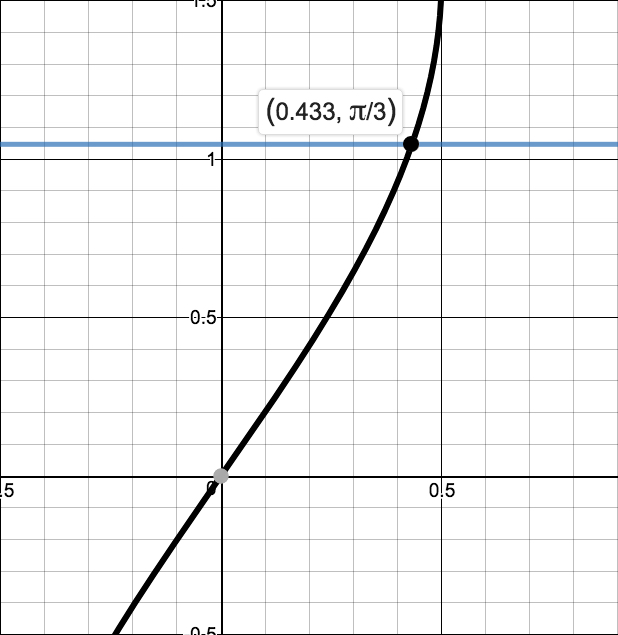
\includegraphics[height=2.5in]{./TrigonometricEquationsandInequalitiesGraphics/ARCSINEQN.jpg}

{\boldmath $y = \arcsin(2x)$} and  $y = \frac{\pi}{3}$

\end{center}

\item Our first step in solving $4\arccos(t)-3\pi = 0$ is to isolate the arccosine. We get $\arccos(t) = \frac{3\pi}{4}$.  Since $\frac{3\pi}{4}$ is in the range of arccosine, we may apply Theorem \ref{arccosinesinefunctionprops}

\[ \begin{array}{rclr}

\arccos(t) & = & \frac{3\pi}{4} & \\ [5pt]
\cos\left(\arccos(t)\right) & = & \cos\left(\frac{3\pi}{4}\right) & \\ [5pt]
t & = & -\frac{\sqrt{2}}{2} & \text{Since $\cos(\arccos(u)) = u$} \\ \end{array} \]


Below we see the graph of $y = 4\arccos(t) - 3\pi$ crosses $y = 0$ at $t=-\frac{\sqrt{2}}{2} \approx -0.7071$.

\begin{center}

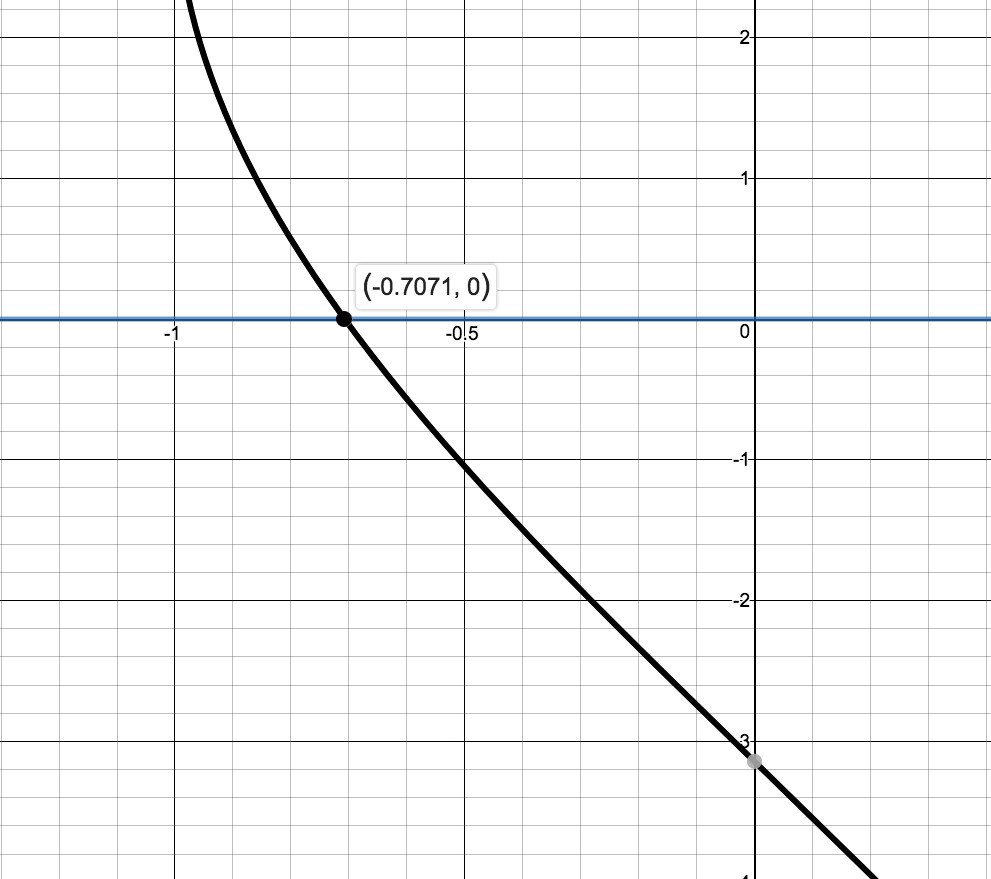
\includegraphics[height=2.5in]{./TrigonometricEquationsandInequalitiesGraphics/ARCCOSEQN.jpg}   

{\boldmath $y=4\arccos(t) - 3\pi$} and $y =0$ \\

\end{center}


\item From $3 \, \text{arcsec}(2x-1) + \pi = 2 \pi$, we get $\text{arcsec}(2x-1) = \frac{\pi}{3}$.  Regardless of how the range of arcsecant is chosen,  since $0 \leq \frac{\pi}{3} < \frac{\pi}{2}$, both Theorems \ref{arcsecantcosecantfunctionprops1}  \ref{arcsecantcosecantfunctionprops2}, apply:

\[ \begin{array}{rclr}

\text{arcsec}(2x-1)& = & \frac{\pi}{3} & \\ [5pt]
\sec(\text{arcsec}(2x-1)) & = & \sec\left(\frac{\pi}{3}\right) & \\ [5pt]
2x -1 & = & 2 & \text{Since $\sec(\text{arcsec}(u)) = u$} \\ [5pt]
    x & = & \frac{3}{2} \\ \end{array} \]

Below we see the graphs of $y=3 \, \text{arcsec}(2x-1) + \pi$ and  $y = 2\pi$ intersect at $x=\frac{3}{2} = 1.5$.

\begin{center}

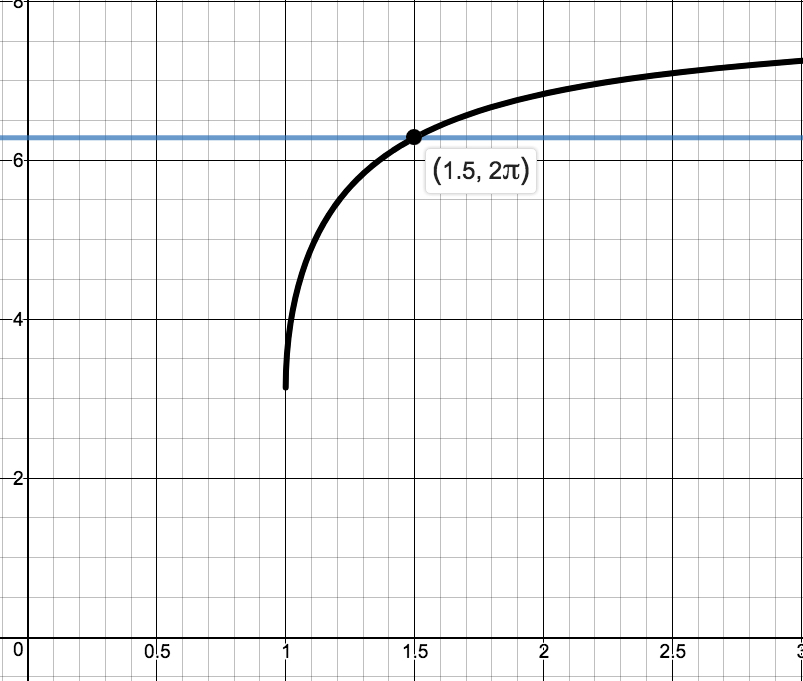
\includegraphics[height=2.5in]{./TrigonometricEquationsandInequalitiesGraphics/ARCSECEQN.jpg} 

{\boldmath $y = 3 \, \text{arcsec}(2x-1) + \pi$} and $y = 2\pi$  

\end{center}

\item  With the presence of both $\arctan^{2}(t)$ ( $= (\arctan(t))^2$) and $\arctan(t)$, we substitute $u = \arctan(t)$ to reveal a quadratic in disguise:  $4u^2 -3\pi u - \pi^2 = 0$.  

\smallskip

Factoring, (don't let the $\pi$ throw you!) we get $(4u+\pi)(u - \pi) = 0$, so $u = \arctan(t) = -\frac{\pi}{4}$ or $u = \arctan(t) = \pi$.  

\smallskip

Since $-\frac{\pi}{4}$ is in the range of arctangent, but $\pi$ is not, we only get solutions from the first equation.  Using Theorem \ref{arctangentcotangentfunctionprops}, we get

\[ \begin{array}{rclr}

\arctan(t) & = & -\frac{\pi}{4} & \\ [5pt]
\tan(\arctan(t)) & = & \tan\left(-\frac{\pi}{4}\right) & \\ [5pt]
t & = & -1 & \text{Since $\tan(\arctan(u)) = u$.} \\ \end{array}\]

We verify this result graphically below.

\begin{center}

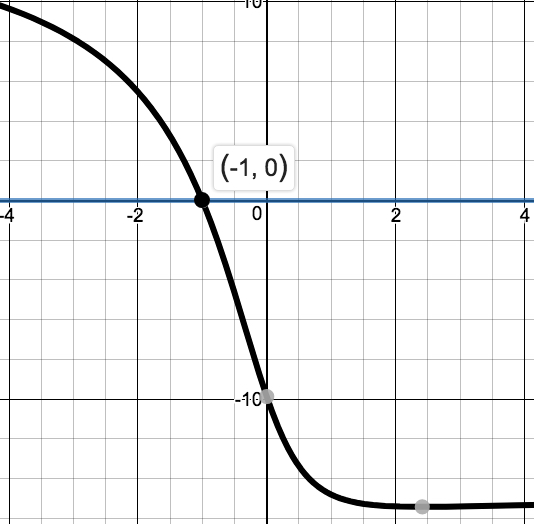
\includegraphics[width=2.2in]{./TrigonometricEquationsandInequalitiesGraphics/ARCTANEQN.jpg}  

{\boldmath  $y=4\arctan^2(t)-3\pi \arctan(t)-\pi^2$ } and $y=0$.\\

\end{center}

\item Since the inverse circular functions are continuous on their domains, we can solve inequalities featuring these functions using sign diagrams. 

\smallskip

Since all of the nonzero terms of  $\pi^2-4\arccos^{2}(x) < 0$ are on one side of the inequality, we let $f(x) = \pi^2-4\arccos^{2}(x)$ and note the domain of $f$ is limited by the $\arccos(x)$ to $[-1,1]$.  

\smallskip

Next, we find the zeros of $f$ by setting $f(x) = \pi^2-4\arccos^{2}(x) = 0$.  We get $\arccos(x) = \pm \frac{\pi}{2}$, and since the range of arccosine is $[0,\pi]$, we focus our attention on $\arccos(x) = \frac{\pi}{2}$.  

\smallskip

Using Theorem \ref{arccosinesinefunctionprops}, we get $x = \cos\left(\frac{\pi}{2}\right) = 0$ as our only zero which breaks our domain $[-1,1]$ into two test intervals: $[-1,0)$ and $(0,1]$.  

\smallskip

Choosing test values $x = \pm 1$, we get $f(-1) = -3\pi^2 < 0$ and $f(1) = \pi^2 > 0$.  Since we are looking for where $f(x) = \pi^2-4\arccos^{2}(x) < 0$, our answer is $[-1,0)$.  

\smallskip

Geometrically,  we find the graph of $y = \pi^2-4\arccos^{2}(x)$ is below $y = 0$ (the $x$-axis) on $[-1,0)$.


\begin{center}

\begin{mfpic}[10]{-5}{5}{-2}{2}
\polyline{(-5,0),(5,0)}
\xmarks{-5,0,5}
\tiny
\tlpointsep{6pt}
\normalsize
\tlabel[cc](-5,-1){$-1$}
\tlabel[cc](-2.5,1){$(-)$}
\tlabel[cc](0,1){$0$}
\tlabel[cc](0,-1){$0$}
\tlabel[cc](5,-1){$1$}
\tlabel[cc](2.5,1){$(+)$}
\end{mfpic} 


 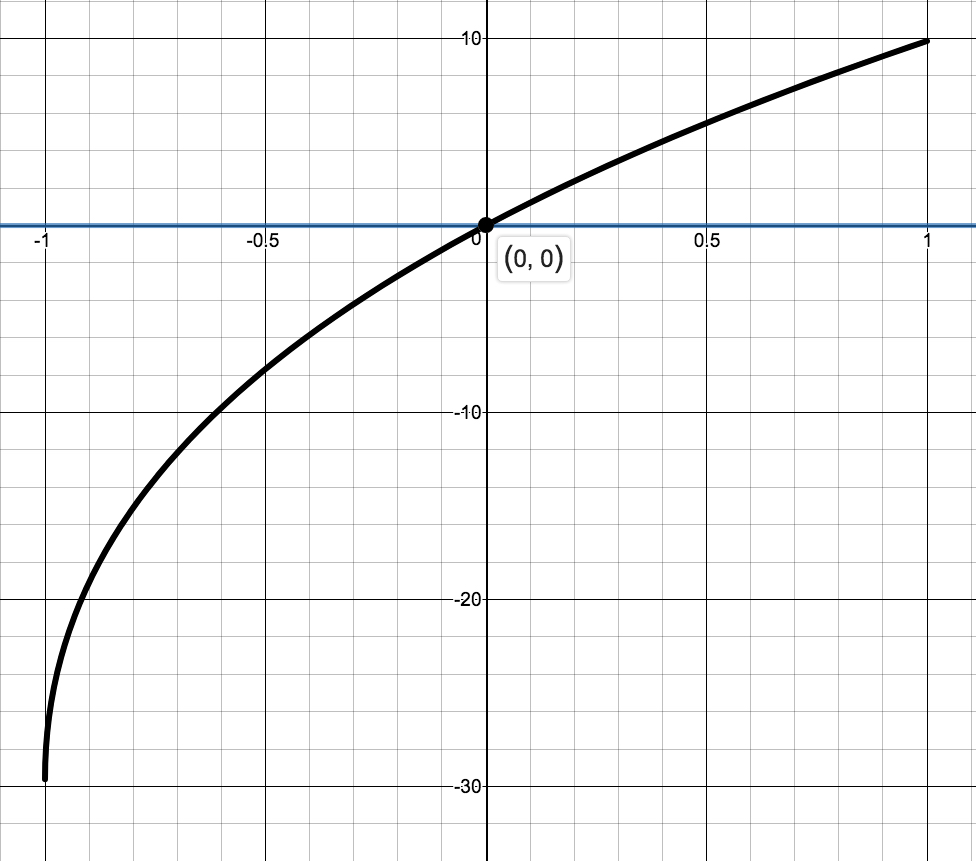
\includegraphics[height=2.5in]{./TrigonometricEquationsandInequalitiesGraphics/ARCCOSINEQ.jpg} \\

{\boldmath $y = \pi^2-4\arccos^{2}(x)$} and $y=0$  

\end{center}

\item   As in the previous problem, we will use a sign diagram to solve $4 \, \text{arccot}(3t) > \pi$.  Our first step is to rewrite the inequality as $4 \, \text{arccot}(3t) -  \pi > 0$. 

\smallskip

We let $f(t) = 4 \, \text{arccot}(3t) -  \pi$, and find the domain of $f$ is all real numbers, $(-\infty, \infty)$.  

\smallskip

To find the zeros of $f$, we set $f(t) = 4 \, \text{arccot}(3t) -  \pi = 0$ and solve.  We get $\text{arccot}(3t) = \frac{\pi}{4}$, and since $\frac{\pi}{4}$ is in the range of arccotangent, we may apply Theorem \ref{arctangentcotangentfunctionprops} and solve 

\[ \begin{array}{rclr}

\text{arccot}(3t) & = & \frac{\pi}{4} & \\ [5pt]
\cot(\text{arccot}(3t)) & = & \cot\left(\frac{\pi}{4}\right) & \\ [5pt]
3t & = & 1 & \text{Since $\cot(\text{arccot}(u)) = u$.} \\ [5pt]
t & = & \frac{1}{3} &  \\ \end{array}\]


Next, we make a sign diagram for $f$.  Since the domain of $f$ is all real numbers, and there is only one zero of $f$, $t = \frac{1}{3}$, we have two test intervals, $\left(-\infty, \frac{1}{3}\right)$ and  $\left(\frac{1}{3}, \infty \right)$.

\smallskip

 Ideally, we wish to find test values $t$ in these intervals so that $\text{arccot}(3t)$ corresponds to one of our oft-used `common' angles.  After a bit of computation,\footnote{Set $3t$ equal to the cotangents of the `common angles' and choose accordingly.} we choose $t=0$ for the interval  $\left(-\infty, \frac{1}{3}\right)$ and $t = \frac{\sqrt{3}}{3}$ for the interval $\left(\frac{1}{3}, \infty \right)$.
 
 \smallskip
 
 We find $f(0) = \pi > 0$ and $f\left(\frac{\sqrt{3}}{3}\right) = -\frac{\pi}{3} < 0$.  Since we are looking for where $f(t) > 0$, we get our answer $\left(-\infty, \frac{1}{3}\right)$.   Graphically, we see  the graph of $y = 4 \, \text{arccot}(3t)$  is above the horizontal line $y = \pi$ on $\left(-\infty, \frac{1}{3}\right)= \left(-\infty, 0.\overline{3} \right)$.



\begin{center}

\begin{mfpic}[10]{-5}{5}{-2}{2}
\arrow \reverse \arrow \polyline{(-5,0),(5,0)}
\xmarks{0}
\tiny
\tlpointsep{6pt}
\normalsize

\tlabel[cc](-2.5,1){$(+)$}
\tlabel[cc](0,1){$0$}
\tlabel[cc](0,-1){$\frac{1}{3}$}
\tlabel[cc](2.5,1){$(-)$}
\end{mfpic}

 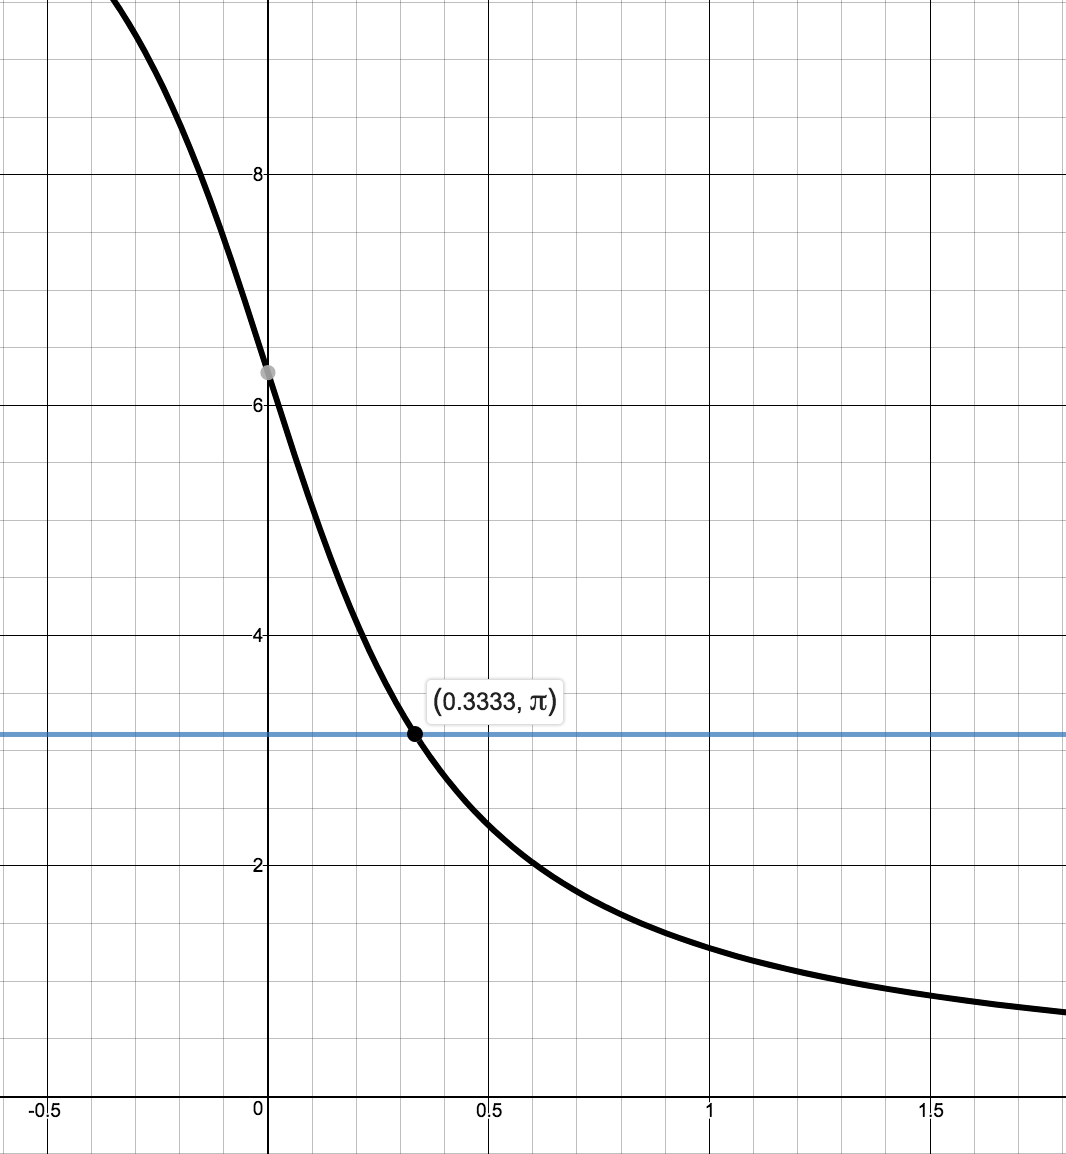
\includegraphics[height=2.5in]{./TrigonometricEquationsandInequalitiesGraphics/ARCCOTINEQ.jpg} 

 { \boldmath $y = 4 \, \text{arccot}(3t)$} and  $y=\pi$ 



\end{center}


\end{enumerate}

\vspace{-.25in} \qed

\end{ex}

\newpage

\subsection{Harmonic Motion}
\label{harmomicmotion}

One of the major applications of the circular functions (sinusoids in particular!)  in Science and Engineering is the study of \index{harmonic motion} \textbf{harmonic motion},  We close this chapter with a brief foray into this topic since it pulls together many important concepts from both Chapters \ref{FoundationsofTrigonometry} and \ref{AnalyticalTrigonometry}.  The equations for harmonic motion can be used to describe a wide range of phenomena, from the motion of an object on a spring, to the response of an electronic circuit.  In this subsection, we restrict our attention to modeling a simple spring system.  Before we jump into the Mathematics, there are some Physics terms and concepts we need to discuss.  

\smallskip

In Physics, `mass' is defined as a measure of an object's resistance to straight-line motion whereas `weight' is the amount of force (pull) gravity exerts on an object.  An object's mass cannot change,\footnote{Well, assuming the object isn't subjected to relativistic speeds \dots} while its weight could change.  An object which weighs 6 pounds on the surface of the Earth would weigh 1 pound on the surface of the Moon, but its mass is the same in both places. In the English system of units, `pounds' (lbs.) is a measure of force (weight), and the corresponding unit of mass is the `slug'. In the SI system, the unit of force is `Newtons' (N) and the associated unit of mass is the `kilogram' (kg). 

\smallskip

We convert between mass and weight using the formula\footnote{This is a consequence of Newton's Second Law of Motion $F = ma$ where $F$ is force, $m$ is mass and $a$ is acceleration.  In our present setting, the force involved is weight which is caused by the acceleration due to gravity.} $w = mg$.   Here, $w$ is the weight of the object, $m$ is the mass and $g$ is the acceleration due to gravity.  In the English system, $g = 32 \frac{\text{feet}}{\text{second}^2}$, and in the SI system, $g = 9.8\frac{\text{meters}}{\text{second}^2}$. Hence, on Earth a \textit{mass} of 1 slug \textit{weighs} 32 lbs. and a \textit{mass} of 1 kg \textit{weighs} 9.8 N.\footnote{Note that $1$ pound $ = 1 \, \frac{\text{slug foot}}{\text{second}^2}$ and $1$ Newton $ = 1 \, \frac{\text{kg meter}}{\text{second}^2}$.}    Suppose we attach an object with mass $m$ to a spring as depicted below. 

\begin{center}

\begin{tabular}[t]{ccc}

\begin{mfpic}[15]{-3}{3}{-2}{5}
\dashed \polyline{(-3,0.5), (3,0.5)}
\hatchcolor[gray]{.7}
\lhatch \rect{(-3,4), (3,5)}
\fillcolor[gray]{.7} 
\gfill \rect{(-0.5,0), (0.5,1)}
\polyline{(0,4), (0,3.5), (0.25,3.25), (-0.25, 3), (0.25,2.75), (-0.25,2.5), (0.25,2.25), (-0.25,2), (0.25,1.75), (-0.25,1.5), (0, 1.25), (0,1)}
\penwd{1.025}
\rect{(-3,4), (3,5)}
\rect{(-0.5,0), (0.5,1)}
\drawcolor{white} \polyline{(-3,-2), (-3,2)}
\end{mfpic} 

&

\hspace{0.5in}
\begin{mfpic}[15]{-3}{3}{-2}{5}
\dashed \polyline{(-3,0.5), (3,0.5)}
\hatchcolor[gray]{.7}
\lhatch \rect{(-3,4), (3,5)}
\fillcolor[gray]{.7} 
\gfill \rect{(-0.5,0.95), (0.5,1.95)}
\polyline{(0,4), (0,3.5), (0.25,3.4), (-0.25, 3.25), (0.25,3.1), (-0.25,2.95), (0.25,2.8), (-0.25,2.65), (0.25,2.5), (-0.25,2.35), (0, 2.2), (0,1.95)}
\penwd{1.025}
\rect{(-3,4), (3,5)}
\rect{(-0.5,0.95), (0.5,1.95)}
\drawcolor{white} \polyline{(-3,-2), (-3,2)}
\end{mfpic} 

&

\hspace{0.5in}
\begin{mfpic}[15]{-3}{3}{-2}{5}
\dashed \polyline{(-3,0.5), (3,0.5)}
\hatchcolor[gray]{.7}
\lhatch \rect{(-3,4), (3,5)}
\fillcolor[gray]{.7} 
\gfill \rect{(-0.5,-1.35), (0.5,-0.35)}
\polyline{(0,4), (0,3.5), (0.25,3.1), (-0.25, 2.7), (0.25,2.3), (-0.25, 1.9), (0.25,1.5), (-0.25,1.1), (0.25,0.7), (-0.25,0.3), (0, -0.1), (0,-0.35)}
\penwd{1.025}
\rect{(-3,4), (3,5)}
\rect{(-0.5,-1.35), (0.5,-0.35)}
\drawcolor{white} \polyline{(-3,-2), (-3,2)}
\end{mfpic} \\
 
$x(t) = 0$ at the &
\hspace{0.5in}
$x(t) < 0$ above the&
\hspace{0.5in}
$x(t) > 0$ below the \\

equilibrium position & 
\hspace{0.5in}
equilibrium position & 
\hspace{0.5in}
equilibrium position \\

\end{tabular}

\end{center}

The weight of the object will stretch the spring.   The system is said to be in `equilibrium' when the weight of the object is perfectly balanced with the restorative force of the spring.  How far the spring stretches to reach equilibrium depends on the spring's `spring constant'. Usually denoted by the letter $k$, the spring constant relates the force $F$ applied to the spring to the amount $d$ the spring stretches in accordance with \href{http://en.wikipedia.org/wiki/Hooke's_law}{\underline{Hooke's Law}}\footnote{Look familiar?  We saw Hooke's Law in Section \ref{AppVariation}.} $F = kd$.  

\smallskip

If the object is released above or below the equilibrium position, or if the object is released with an upward or downward velocity, the object will bounce up and down on the end of the spring until some external force stops it.  If we let $x(t)$ denote the object's displacement from the equilibrium position at time $t$, then $x(t) = 0$ means the object is at the equilibrium position, $x(t) < 0$ means the object is \textit{above} the equilibrium position, and $x(t) > 0$ means the object is \textit{below} the equilibrium position.  The function $x(t)$ is called the `equation of motion' of the object.\footnote{To keep units compatible, if we are using the English system, we use feet (ft.) to measure displacement.  If we are in the SI system, we measure displacement in meters (m). Time is always measured in seconds (s).}

\smallskip


If we ignore all other influences on the system except gravity and the spring force, then Physics tells us that gravity and the spring force will battle each other forever and the object will oscillate indefinitely.  In this case, we describe the motion as `free' (meaning there is no external force causing the motion) and `undamped' (meaning we ignore friction caused by surrounding medium, which in our case is air).  

\smallskip

The following theorem, which comes from Differential Equations, gives $x(t)$ as a function of the mass $m$ of the object, the spring constant $k$, the initial displacement $x_{\text{\tiny $0$}}$ of the object and initial velocity $v_{\text{\tiny $0$}}$ of the object.  

\smallskip

As with $x(t)$, $x_{\text{\tiny $0$}} = 0$ means the object is released from the equilibrium position, $x_{\text{\tiny $0$}} < 0$ means the object is released \textit{above} the equilibrium position and $x_{\text{\tiny $0$}}>0$ means the object is released \textit{below} the equilibrium position.  As far as the initial velocity $v_{\text{\tiny $0$}}$ is concerned, $v_{\text{\tiny $0$}} =0 $ means the object is released `from rest,' $v_{\text{\tiny $0$}}<0$ means the object is heading \textit{upwards} and $v_{\text{\tiny $0$}}>0$ means the object is heading \textit{downwards}.\footnote{The sign conventions here are carried over from Physics.  If not for the spring, the object would fall towards the ground, which is the `natural' or `positive' direction.  Since the spring force acts in direct opposition to gravity,  any movement upwards is considered `negative'.}

\medskip

\colorbox{ResultColor}{\bbm
\begin{thm} \label{freeundampedmotion} \textbf{Equation for Free Undamped Harmonic Motion:}  Suppose an object of  mass $m$ is suspended from a spring with spring constant $k$.  If the initial displacement from the equilibrium position is $x_{\text{\tiny $0$}}$ and the initial velocity of the object is $v_{\text{\tiny $0$}}$, then the displacement $x$ from the equilibrium position at time $t$ is given by  $x(t) = A \sin(\omega t + \phi)$ where

\begin{itemize}

\item  $\omega = \sqrt{\dfrac{k}{m}}$ and $A = \sqrt{x_{\text{\tiny $0$}}^2 + \left( \dfrac{v_{\text{\tiny $0$}}}{\omega}\right)^2}$

\item $A\sin(\phi) = x_{\text{\tiny $0$}}$ and $A\omega\cos(\phi) = v_{\text{\tiny $0$}}$.

\end{itemize} 

\end{thm}

\smallskip

\ebm}

\medskip

It is a great exercise in `dimensional analysis' to verify that the formulas given in Theorem \ref{freeundampedmotion} work out so that $\omega$ has units $\frac{1}{s}$ and  $A$ has units ft. or m, depending on which system we choose.

\begin{ex} \label{freeudampedex}  Suppose an object weighing  64 pounds stretches a spring 8 feet.  

\begin{enumerate}

\item  If the object is attached to the spring and released 3 feet below the equilibrium position from rest, find the equation of motion of the object, $x(t)$.  When does the object first pass through the equilibrium position?  Is the object heading upwards or downwards at this instant? 

\item  If the object is attached to the spring and released 3 feet below the equilibrium position with an upward velocity of $8$ feet  per second, find the equation of motion of the object, $x(t)$.  What is the longest distance the object travels \textit{above} the equilibrium position?  When does this first happen? Confirm your result using a graphing utility.

\end{enumerate}

{\bf Solution.} In order to use the formulas in Theorem \ref{freeundampedmotion}, we first need to determine the spring constant $k$ and the mass of the object $m$.  

\smallskip

To find $k$, we use Hooke's Law $F = kd$.  We know the object weighs $64$ lbs. and stretches the spring $8$ ft.. Using $F = 64$ and $d = 8$,  we get  $64  = k \cdot 8 $, or  $k = 8 \frac{\text{lbs.}}{\text{ft.}}$.  

\smallskip

To find $m$, we use $w = mg$ with $w = 64$ lbs. and $g =32 \frac{\text{ft.}}{s^2}$.  We get $m = 2$ slugs.  We can now proceed to apply Theorem \ref{freeundampedmotion}.

\begin{enumerate}

\item  With $k = 8$ and $m = 2$, we get $\omega = \sqrt{\frac{k}{m}} = \sqrt{\frac{8}{2}} = 2$.  Since the object is released 3 feet \textit{below} the equilibrium position `from rest,'    $x_{\text{\tiny $0$}} = 3$ and  $v_{\text{\tiny $0$}} = 0$.  Therefore, $A = \sqrt{x_{\text{\tiny $0$}}^2 + \left( \frac{v_{\text{\tiny $0$}}}{\omega}\right)^2} = \sqrt{3^2 + 0^2} = 3$.  

\smallskip

 To determine the phase $\phi$, we have $A\sin(\phi) = x_{\text{\tiny $0$}}$, which in this case gives $3 \sin(\phi) = 3$ so $\sin(\phi) = 1$.  Only $\phi = \frac{\pi}{2}$ and angles coterminal to it satisfy this condition, so we pick\footnote{For confirmation, we note that $A\omega\cos(\phi) = v_{\text{\tiny $0$}}$, which in this case reduces to $6\cos(\phi) = 0$.} the phase to be $\phi = \frac{\pi}{2}$.  Hence, the equation of motion is $x(t) = 3\sin\left(2t + \frac{\pi}{2}\right)$.  

\smallskip

To find when the object passes through the equilibrium position we solve $x(t)= 3\sin\left(2t + \frac{\pi}{2}\right) = 0$. Going through the usual analysis we find $t = -\frac{\pi}{4} + \frac{\pi}{2} k$ for integers $k$. Since we are interested in the \textit{first} time the object passes through the equilibrium position, we look for the smallest positive $t$ value which in this case is $t = \frac{\pi}{4} \approx 0.78$ seconds after the  start of the motion.  

\smallskip

Common sense suggests that if we release the object \textit{below} the equilibrium position, the object should be traveling \textit{upwards} when it first passes through it.   To check this answer, we graph one cycle of  $x(t)$.  Since our applied domain in this situation is $t \geq 0$, and the period of $x(t)$ is $T = \frac{2\pi}{\omega} = \frac{2\pi}{2} = \pi$, we graph $x(t)$ over the interval $[0,\pi]$.  Remembering that $x(t) > 0$ means the object is below the equilibrium position and $x(t) < 0$ means the object is above the equilibrium position, the fact our graph is crossing through the $t$-axis from positive $x$ to negative $x$ at $t = \frac{\pi}{4}$ confirms our answer.


\begin{center}

\begin{mfpic}[30][15]{-0.5}{4}{-3.25}{3.5}

\axes
\point[4pt]{(0,3), (0.78,0), (1.57,-3), (2.36,0), (3.14,3)}
\tlabel[cc](4,-0.5){\scriptsize $t$}
\tlabel[cc](0.5,3.5){\scriptsize $x$}
\xmarks{0.78, 1.57, 2.36, 3.14}
\ymarks{-3,-2,-1,1,2,3}
\tlabelsep{5pt}
\scriptsize
\axislabels{x}{{$\frac{\pi}{4}\hspace{7pt}$} 0.78, {$\frac{\pi}{2}$} 1.57,{$\frac{3\pi}{4}$} 2.36, {$\pi$} 3.14}
\axislabels{y}{{$-3$} -3, {$-2$} -2,{$-1$} -1, {$1$} 1,{$2$} 2,{$3$} 3}
\normalsize
\penwd{1.25pt}
\arrow \function{0, 0.65, 0.1}{3*sin(2*x+1.57)}
\arrow \function{0.65, 1, 0.1}{3*sin(2*x+1.57)}
\function{1, 3.14, 0.1}{3*sin(2*x+1.57)}
\end{mfpic}

$x(t)= 3\sin\left(2t + \frac{\pi}{2}\right)$

\end{center}

\item  The only difference between this problem and the previous problem is that we now release the object with an upward velocity of $8 \, \frac{\text{ft}}{s}$.  We still have $\omega = 2$ and $x_{\text{\tiny $0$}} = 3$, but now we have $v_{\text{\tiny $0$}} = -8$, the negative indicating the velocity is directed upwards. 

\smallskip

Here, we get $A = \sqrt{x_{\text{\tiny $0$}}^2 + \left( \frac{v_{\text{\tiny $0$}}}{\omega}\right)^2} = \sqrt{3^2 + (-4)^2} = 5$.  From $A\sin(\phi) = x_{\text{\tiny $0$}}$, we get $5\sin(\phi) = 3$ which gives $\sin(\phi) = \frac{3}{5}$.  From  $A\omega\cos(\phi) = v_{\text{\tiny $0$}}$, we get $10\cos(\phi) = -8$, or $\cos(\phi) = -\frac{4}{5}$.  

\smallskip

Hence,  $\phi$ is a Quadrant II angle which we can describe in terms of either arcsine or arccosine.  Since the range of arccosine covers Quadrant II, we choose to express $\phi$ in terms of the arccosine:  $\phi = \arccos\left( -\frac{4}{5} \right)$.  Hence, $x(t)= 5 \sin\left(2t + \arccos\left(-\frac{4}{5}\right) \right)$.  

\smallskip

Since the amplitude of $x(t)$ is $5$, the object will travel at most $5$ feet above the equilibrium position.  To find when this happens, we solve the equation $x(t)= 5 \sin\left(2t +\arccos\left( -\frac{4}{5} \right) \right)= -5$, the negative once again signifying that the object is \textit{above} the equilibrium position.  

\smallskip

Going through the usual machinations, we get $t = -\frac{1}{2} \arccos\left( -\frac{4}{5} \right)-\frac{\pi}{4}  + \pi k$ for integers $k$. The smallest (positive) of these values occurs when $k=1$, that is, $t =-\frac{1}{2} \arccos\left( -\frac{4}{5} \right)+ \frac{3\pi}{4}  \approx 1.107$ seconds after the start of the motion. 

\smallskip

Graphing $x(t) = 5 \sin\left(2t +  \arccos\left( -\frac{4}{5} \right) \right)$, we find the coordinates of the first relative minimum of to be approximately $(1.107,-5)$ .



\begin{center}


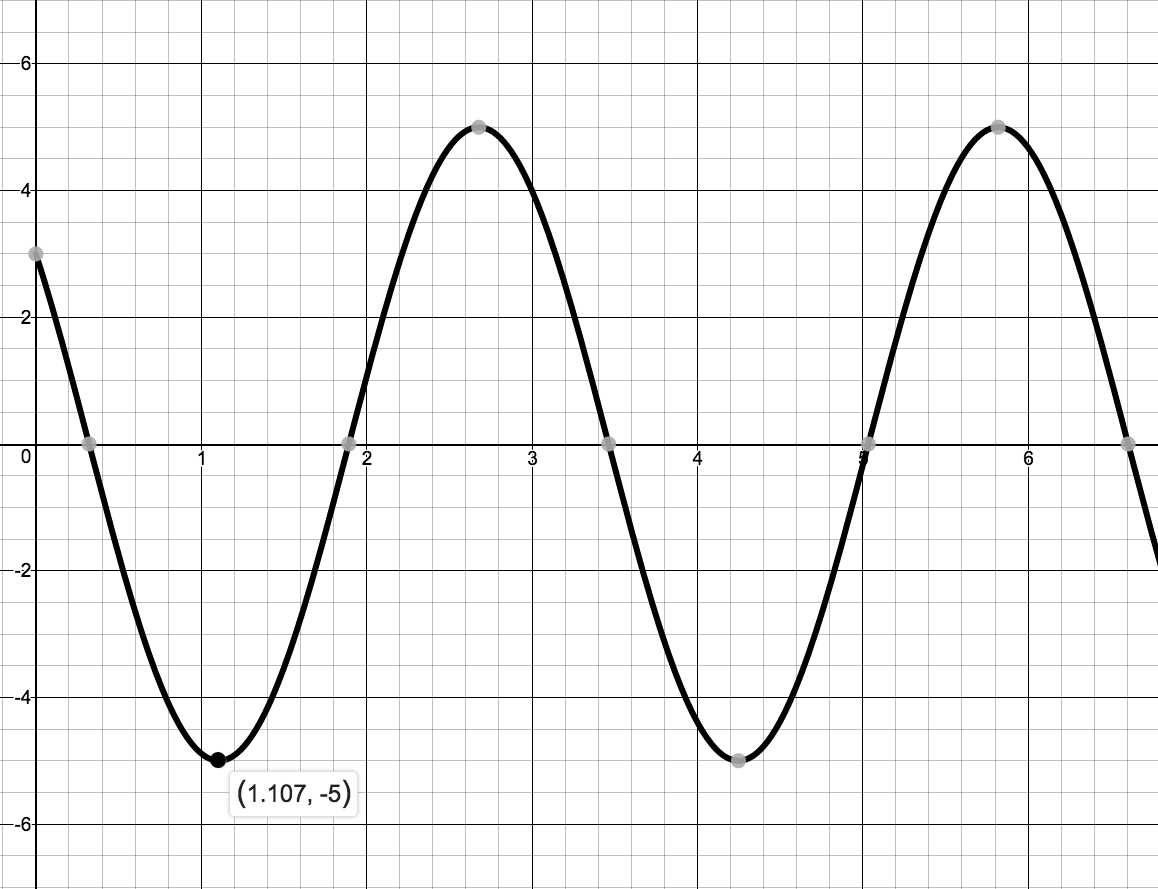
\includegraphics[height=2.5in]{./TrigonometricEquationsandInequalitiesGraphics/Sinusoid05.jpg} 

 $x(t) = 5 \sin\left(2t +  \arccos\left( -\frac{4}{5} \right) \right)$



\end{center}

\qed

\end{enumerate}
\end{ex}

Though beyond the scope of this course, it is possible  to model the effects of friction and other external forces acting on the system.\footnote{Take a good Differential Equations class to see this!}  

\smallskip

While we may not have the Physics and Calculus background to \textit{derive} equations of motion for these scenarios, we can certainly analyze them.  We examine three cases in the following example.

\newpage

\begin{ex} \label{underdampedresonance}  $~$  

\begin{enumerate}

\item  Write $x(t) = 5e^{-t/5} \cos(t) + 5e^{-t/5} \sqrt{3} \sin(t)$ in the form $x(t) = A(t) \sin(\omega t + \phi)$.  Graph $x(t)$ using a graphing utility.

\item  Write $x(t) = (t+3)\sqrt{2} \cos(2t) + (t+3) \sqrt{2} \sin(2t)$ in the form $x(t) = A(t) \sin(\omega t + \phi)$.  Graph $x(t)$  using a graphing utility.

\item  Find the period of $x(t) = 5\sin(6t) - 5\sin\left(8t\right)$.  Graph $x(t)$ using a graphing utility.

\end{enumerate}

{\bf Solution.}

\begin{enumerate}

\item  We start rewriting  $x(t) = 5e^{-t/5} \cos(t) + 5e^{-t/5} \sqrt{3} \sin(t)$ by factoring out   $5e^{-t/5}$ from both terms to get  $x(t) = 5e^{-t/5} \left( \cos(t) + \sqrt{3} \sin(t)\right)$. We convert what's left in parentheses to the required form using the technique introduced in Example  \ref{expandedsinusoid} from Section \ref{MoreTrigonometricIdentities}.  We find $\left( \cos(t) + \sqrt{3} \sin(t)\right) = 2\sin\left(t+\frac{\pi}{3}\right)$ so that $x(t) = 10e^{-t/5} \sin\left(t + \frac{\pi}{3}\right)$.    


\smallskip

Graphing $x(t)$ reveals some interesting behavior.  The sinusoidal nature continues indefinitely, but it is being attenuated.  In the sinusoid $A \sin(\omega t + \phi)$, the coefficient $A$ of the sine function is the amplitude.  In the case of $x(t) = 10e^{-t/5} \sin\left(t + \frac{\pi}{3}\right)$, we can think of the \textit{function} $A(t) = 10e^{-t/5}$ as the amplitude.\footnote{This is the same sort of phenomenon we saw on page \pageref{beats} in Section \ref{expandedsinusoid}.}  As $t \rightarrow \infty$, $10e^{-t/5} \rightarrow 0$ which means the amplitude shrinks towards zero. 

Indeed, if we graph $x = \pm 10e^{-t/5}$ along with $x(t) = 10e^{-t/5} \sin\left(t + \frac{\pi}{3}\right)$, we see this attenuation taking place with the exponentials acting as a `wave envelope.'  

\begin{center}

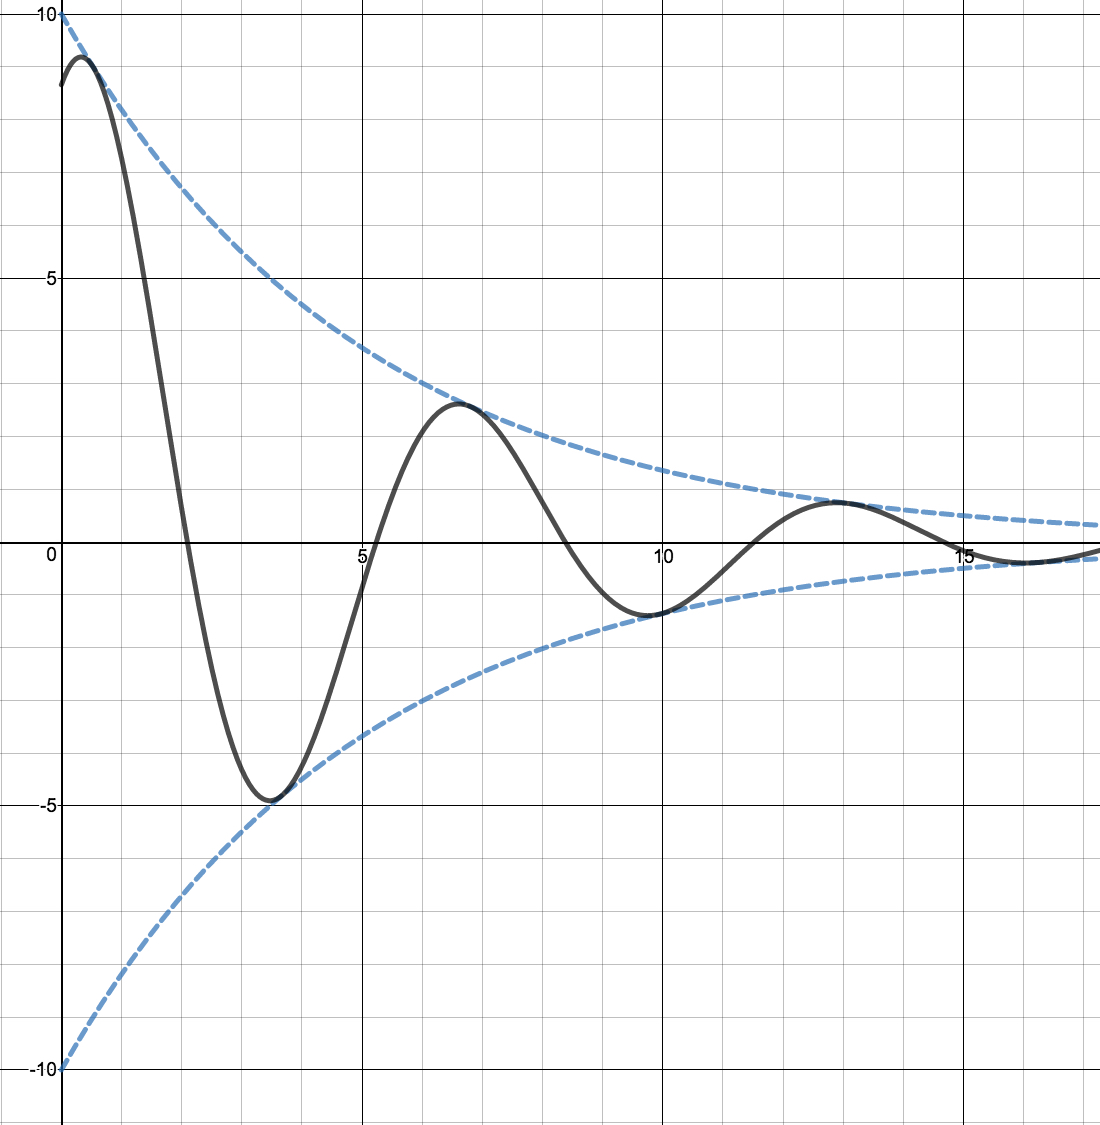
\includegraphics[height=2.5in]{./TrigonometricEquationsandInequalitiesGraphics/Sinusoid06.jpg} 

{\boldmath $x(t) = 10e^{-t/5} \sin\left(t + \frac{\pi}{3}\right)$} and $x= \pm 10e^{-t/5}$ \\

\end{center}

In this case, the function $x(t)$  corresponds to the motion of an object on a spring where there is a slight force which acts to `damp', or slow the motion.  An example of this kind of force would be the friction of the object against the air. According to  this model, the object oscillates forever, but with increasingly smaller and smaller amplitude. 


\item  Proceeding as in the first example, we factor out $(t+3)\sqrt{2}$ from each term in the function $x(t)$ to get $x(t) = (t+3)\sqrt{2}(\cos(2t) + \sin(2t))$.   We find $(\cos(2t) + \sin(2t)) = \sqrt{2} \sin\left(2t + \frac{\pi}{4}\right)$, so an equivalent form of $x(t)$ is  $x(t) = 2(t+3) \sin\left(2t + \frac{\pi}{4}\right)$.  

\smallskip

Graphing $x(t)$, we find the sinusoid's amplitude growing.  This isn't too surprising  since our amplitude function here is $A(t) = 2(t+3) = 2t+6$, grows without bound as $t \rightarrow \infty$.  


\begin{center}

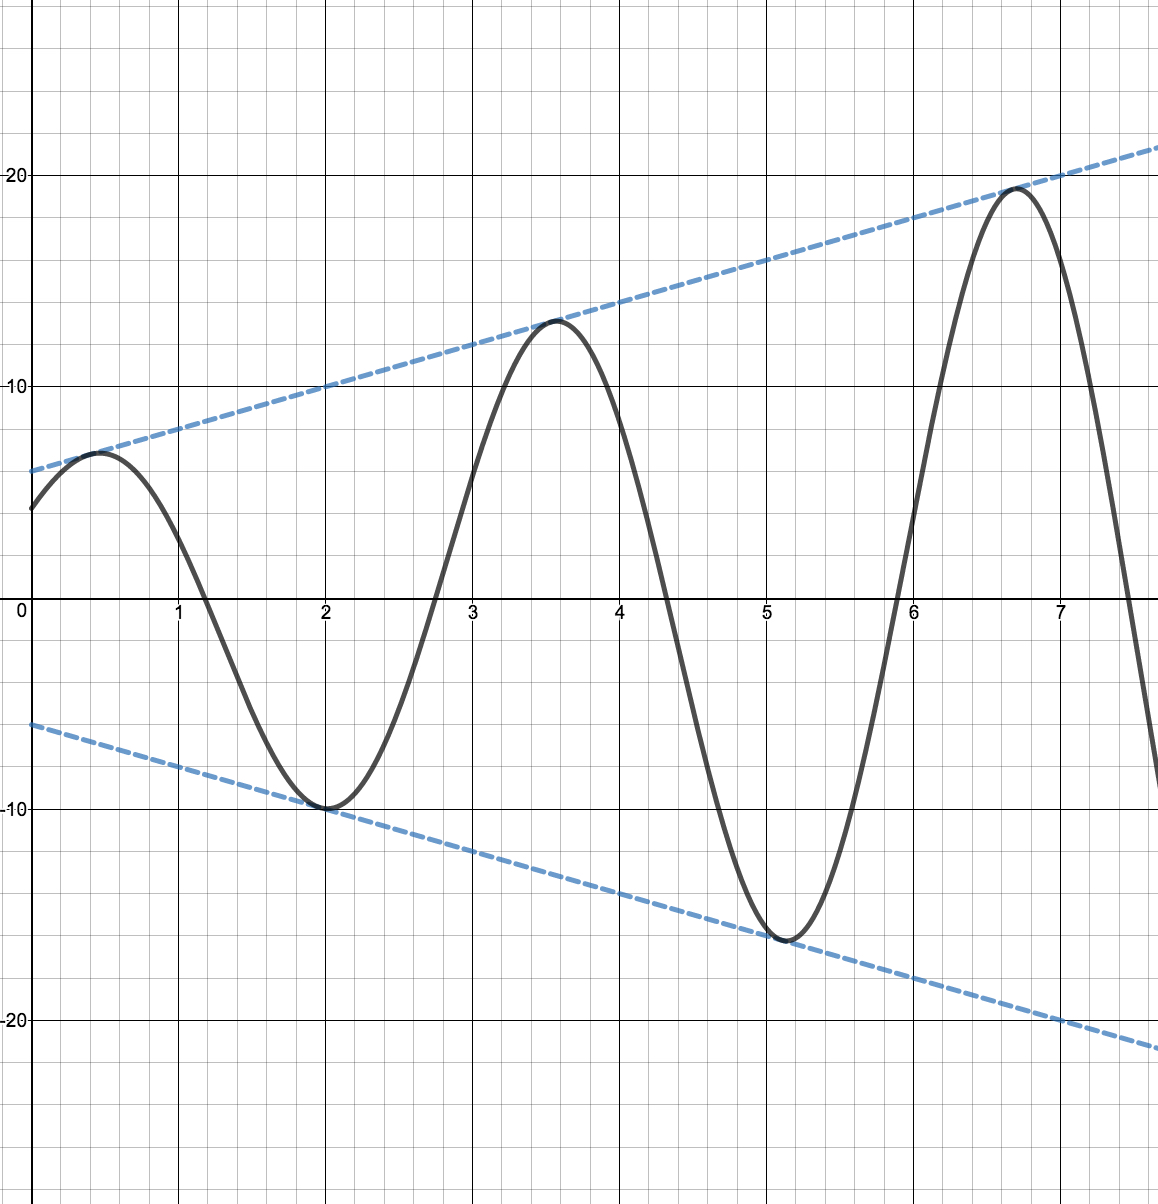
\includegraphics[height=2.5in]{./TrigonometricEquationsandInequalitiesGraphics/Sinusoid08.jpg} 

{\boldmath $x(t)= 2(t+3) \sin\left(2t + \frac{\pi}{4}\right)$} and $x = \pm 2(t+3)$ \\



\end{center}

The phenomenon illustrated here is `forced' motion.  That is, we imagine that the entire apparatus on which the spring is attached is oscillating as well.  

\smallskip

In this particular case, we are witnessing a `resonance' effect -- the frequency of the external oscillation matches the frequency of the motion of the object on the spring. In a mechanical system, this will result in some sort of structural failure.\footnote{The reader is invited to investigate the destructive implications of \href{http://en.wikipedia.org/wiki/Resonance}{\underline{resonance}}.}



\vspace{-.1in}

\item Last, but not least, we come to  $x(t) = 5\sin(6t) - 5\sin(8t)$.  To find the period of this function, we need to determine the length of the smallest interval on which both $f(t) = 5\sin(6t)$ and $g(t) = 5\sin(8t)$ complete a whole number of cycles. 

\smallskip

To do this, we take the ratio of their frequencies and reduce to lowest terms:  $\frac{6}{8} = \frac{3}{4}$.  This tells us that for every $3$ cycles $f$ makes, $g$ makes $4$. Hence,  the period of $x(t)$ is three times the period of $f(t)$ (which is four times the period of $g(t)$), or $\pi$.   We check our work by graphing $x(t)$  over  $[0,\pi]$

\smallskip

The reader may recognize $x(t)$  an example of the `beats' phenomenon we first saw on \pageref{beats} in Section \ref{expandedsinusoid}.  Indeed, using a sum to product identity, we may rewrite $x(t)$ as $x(t) =  -10 \sin(t) \cos(7t)$.  As we saw on \pageref{beats}  (and Exercises \ref{beatexfirst} - \ref{beatexlast} in Section \ref{MoreTrigonometricIdentities}), the lower frequency factor, $-10\sin(t)$ determines the `wave-envelope,'   $x = \pm 10 \sin(t)$.  


\begin{center}

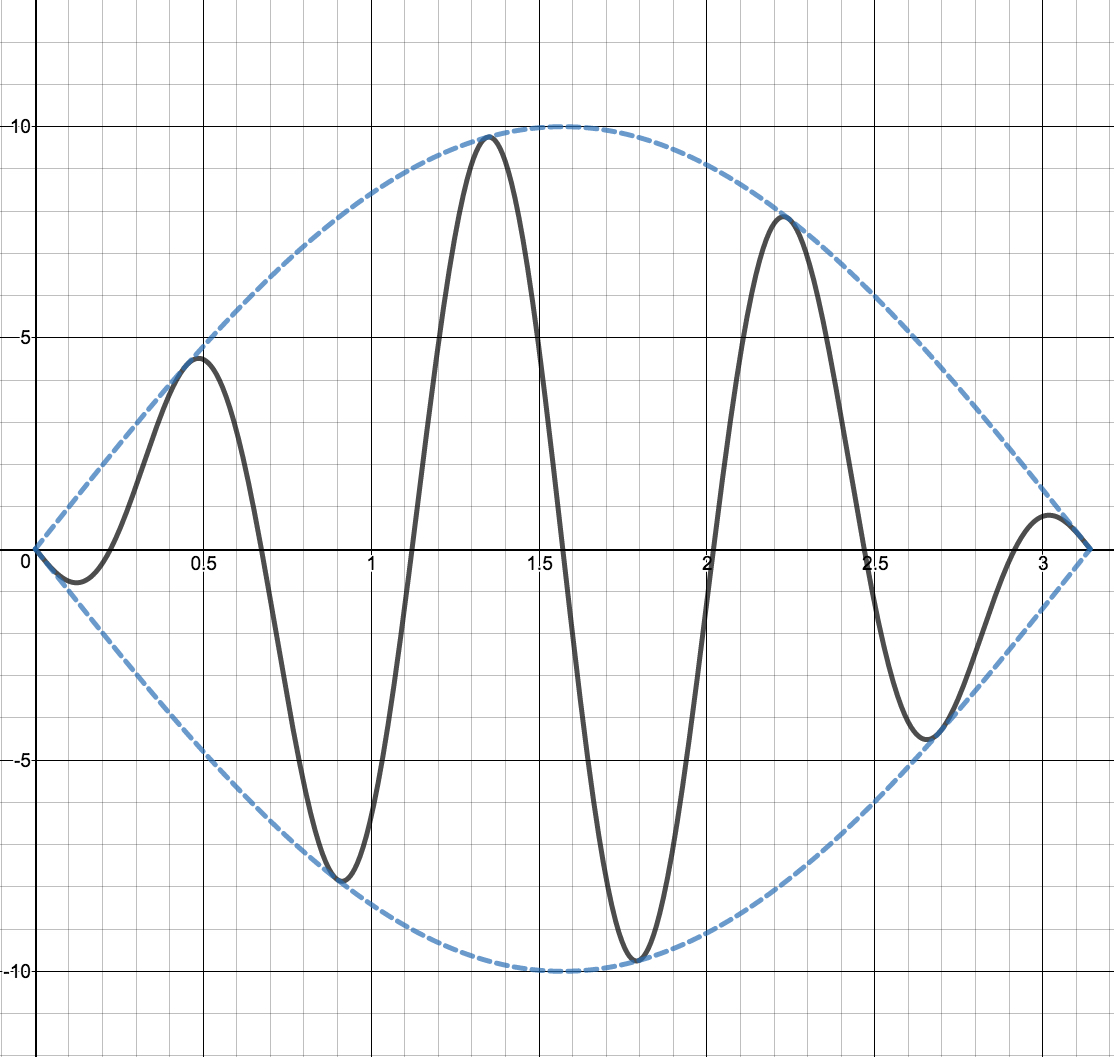
\includegraphics[height=2.5in]{./TrigonometricEquationsandInequalitiesGraphics/Sinusoid10.jpg} 


{\boldmath $x(t) = 5\sin(6t) - 5\sin(8t)$} and  $x = \pm 10 \sin(t)$ over $[0,\pi]$



\end{center}

 This equation of motion also results from `forced' motion, but here the frequency of the external oscillation is different than that of the object on the spring.  Since the sinusoids here have different frequencies, they are `out of sync' and  do not amplify each other as in the previous example.  Instead, through a combination of constructive and destructive interference, the mass continues to oscillate no more than $10$ units from its equilibrium position indefinitely.  \qed


\end{enumerate}

\end{ex}

\newpage

\subsection{Exercises}
In Exercises \ref{solvebasicfirst} - \ref{solvebasiclast}, find \underline{all} of the exact solutions of the  equation and then list those solutions which are in the interval $[0, 2\pi)$.

\begin{multicols}{3}

\begin{enumerate}

\item $\sin \left( 5 \theta \right) = 0$ \vphantom{$\dfrac{\sqrt{3}}{2}$} \label{solvebasicfirst}
\item $\cos \left( 3t \right) = \dfrac{1}{2}$ \vphantom{$\dfrac{\sqrt{3}}{2}$}
\item $\sin \left( -2x \right) = \dfrac{\sqrt{3}}{2}$ 

\setcounter{HW}{\value{enumi}}

\end{enumerate}

\end{multicols}

\begin{multicols}{3}

\begin{enumerate}

\setcounter{enumi}{\value{HW}}

\item $\tan \left( 6 \theta \right) = 1$
\item $\csc \left( 4 t \right) = -1$
\item $\sec \left( 3x \right) = \sqrt{2}$

\setcounter{HW}{\value{enumi}}

\end{enumerate}

\end{multicols}

\begin{multicols}{3}

\begin{enumerate}

\setcounter{enumi}{\value{HW}}

\item $\cot \left( 2 \theta \right) = -\dfrac{\sqrt{3}}{3}$
\item $\cos \left( 9t  \right) = 9$ \vphantom{$\dfrac{\sqrt{3}}{2}$}
\item $\sin \left( \dfrac{x}{3} \right) = \dfrac{\sqrt{2}}{2}$

\setcounter{HW}{\value{enumi}}

\end{enumerate}

\end{multicols}

\begin{multicols}{3}

\begin{enumerate}

\setcounter{enumi}{\value{HW}}

\item $\cos \left( \theta+ \dfrac{5\pi}{6} \right) = 0$
\item $\sin \left( 2t - \dfrac{\pi}{3} \right) = -\dfrac{1}{2}$
\item $2\cos \left( x + \dfrac{7\pi}{4} \right) = \sqrt{3}$

\setcounter{HW}{\value{enumi}}

\end{enumerate}

\end{multicols}

\begin{multicols}{3}

\begin{enumerate}

\setcounter{enumi}{\value{HW}}

\item $\csc( \theta) = 0$
\item $\tan \left( 2t - \pi \right) = 1$
\item $\tan^{2} \left( x \right) = 3$

\setcounter{HW}{\value{enumi}}

\end{enumerate}

\end{multicols}

\begin{multicols}{3}

\begin{enumerate}

\setcounter{enumi}{\value{HW}}

\item $\sec^{2} \left( \theta \right) = \dfrac{4}{3}$
\item $\cos^{2} \left( t \right) = \dfrac{1}{2}$
\item $\sin^{2} \left( x \right) = \dfrac{3}{4}$ \label{solvebasiclast}

\setcounter{HW}{\value{enumi}}

\end{enumerate}

\end{multicols}

In Exercises \ref{solveidentfirst} - \ref{solveidentlast}, solve the equation, giving the exact solutions which lie in $[0, 2\pi)$


\begin{multicols}{2}

\begin{enumerate}

\setcounter{enumi}{\value{HW}}

\item $\sin \left( \theta \right) = \cos \left( \theta \right)$ \label{solveidentfirst}
\item $\sin \left( 2t \right) = \sin \left( t \right)$

\setcounter{HW}{\value{enumi}}

\end{enumerate}

\end{multicols}

\begin{multicols}{2}

\begin{enumerate}

\setcounter{enumi}{\value{HW}}

\item $\sin \left( 2x \right) = \cos \left( x \right)$
\item $\cos \left( 2\theta \right) = \sin \left( \theta \right)$

\setcounter{HW}{\value{enumi}}

\end{enumerate}

\end{multicols}

\begin{multicols}{2}

\begin{enumerate}

\setcounter{enumi}{\value{HW}}

\item $\cos \left( 2t \right) = \cos \left( t \right)$
\item  $\cos(2x) = 2 - 5\cos(x)$

\setcounter{HW}{\value{enumi}}

\end{enumerate}

\end{multicols}

\begin{multicols}{2}

\begin{enumerate}

\setcounter{enumi}{\value{HW}}

\item  $3\cos(2 \theta ) + \cos(\theta) + 2 = 0$
\item  $\cos(2t) = 5\sin(t) - 2$

\setcounter{HW}{\value{enumi}}

\end{enumerate}

\end{multicols}

\begin{multicols}{2}

\begin{enumerate}

\setcounter{enumi}{\value{HW}}

\item  $3\cos(2x) = \sin(x) + 2$
\item  $2\sec^{2}(\theta) = 3 - \tan(\theta)$

\setcounter{HW}{\value{enumi}}

\end{enumerate}

\end{multicols}

\begin{multicols}{2}

\begin{enumerate}

\setcounter{enumi}{\value{HW}}

\item  $\tan^{2}(t) = 1-\sec(t)$
\item  $\cot^{2}(x) = 3\csc(x) - 3$

\setcounter{HW}{\value{enumi}}

\end{enumerate}

\end{multicols}

\begin{multicols}{2}

\begin{enumerate}

\setcounter{enumi}{\value{HW}}

\item  $\sec(\theta) = 2\csc(\theta)$
\item  $\cos(t) \csc(t)\cot(t) = 6-\cot^{2}(t)$

\setcounter{HW}{\value{enumi}}

\end{enumerate}

\end{multicols}

\begin{multicols}{2}

\begin{enumerate}

\setcounter{enumi}{\value{HW}}

\item  $\sin(2x) = \tan(x)$
\item  $\cot^{4}(\theta) = 4\csc^{2}(\theta) - 7$

\setcounter{HW}{\value{enumi}}

\end{enumerate}

\end{multicols}

\begin{multicols}{2}

\begin{enumerate}

\setcounter{enumi}{\value{HW}}

\item  $\cos(2t) + \csc^{2}(t) = 0$
\item $\tan^{3} \left( x \right) = 3\tan \left( x \right)$

\setcounter{HW}{\value{enumi}}

\end{enumerate}

\end{multicols}

\begin{multicols}{2}

\begin{enumerate}

\setcounter{enumi}{\value{HW}}

\item $\tan^{2} \left( \theta \right) = \dfrac{3}{2} \sec \left( \theta \right)$
\item $\cos^{3} \left( t \right) = -\cos \left( t \right)$ \vphantom{$\dfrac{3}{2}$}

\setcounter{HW}{\value{enumi}}

\end{enumerate}

\end{multicols}

\begin{multicols}{2}

\begin{enumerate}

\setcounter{enumi}{\value{HW}}

\item $\tan (2x) - 2\cos(x) = 0$
\item $\csc^{3}(\theta) + \csc^{2}(\theta) = 4\csc(\theta) + 4$

\setcounter{HW}{\value{enumi}}

\end{enumerate}

\end{multicols}

\enlargethispage{0.35in}
\vspace{-0.15in}

\begin{multicols}{2}

\begin{enumerate}

\setcounter{enumi}{\value{HW}}

\item $2\tan(t) = 1 - \tan^{2}(t)$
\item $\tan \left( x \right) = \sec \left( x \right)$ \label{solveidentlast}

\setcounter{HW}{\value{enumi}}

\end{enumerate}

\end{multicols}

\pagebreak

In Exercises \ref{solvemoreidentfirst} - \ref{solvemoreidentlast}, solve the equation, giving the exact solutions which lie in $[0, 2\pi)$


\begin{multicols}{2}

\begin{enumerate}

\setcounter{enumi}{\value{HW}}

\item $\sin(6\theta) \cos(\theta) = -\cos(6\theta) \sin(\theta)$ \label{solvemoreidentfirst}
\item  $\sin(3t)\cos(t) = \cos(3t) \sin(t)$

\setcounter{HW}{\value{enumi}}

\end{enumerate}

\end{multicols}

\begin{multicols}{2}

\begin{enumerate}

\setcounter{enumi}{\value{HW}}

\item $\cos(2x)\cos(x) + \sin(2x)\sin(x) = 1$ \vphantom{$\dfrac{\sqrt{3}}{2}$}
\item \small $\cos(5\theta)\cos(3\theta) - \sin(5\theta)\sin(3\theta) = \dfrac{\sqrt{3}}{2}$ \normalsize

\setcounter{HW}{\value{enumi}}

\end{enumerate}

\end{multicols}

\begin{multicols}{2}

\begin{enumerate}

\setcounter{enumi}{\value{HW}}

%Sinusoids
\item $\sin(t) + \cos(t) = 1$
\item  $\sin(x) + \sqrt{3} \cos(x) = 1$

\setcounter{HW}{\value{enumi}}

\end{enumerate}

\end{multicols}

\begin{multicols}{2}

\begin{enumerate}

\setcounter{enumi}{\value{HW}}

\item  $\sqrt{2} \cos(\theta) - \sqrt{2} \sin(\theta) = 1$
\item  $\sqrt{3} \sin(2t) +  \cos(2t) = 1$

\setcounter{HW}{\value{enumi}}

\end{enumerate}

\end{multicols}

\begin{multicols}{2}

\begin{enumerate}

\setcounter{enumi}{\value{HW}}

\item $\cos(2x) - \sqrt{3} \sin(2x) = \sqrt{2}$
\item $3\sqrt{3}\sin(3\theta) - 3\cos(3\theta) = 3\sqrt{3}$

\setcounter{HW}{\value{enumi}}

\end{enumerate}

\end{multicols}

\begin{multicols}{2}

\begin{enumerate}

\setcounter{enumi}{\value{HW}}

\item  $\cos(3t) = \cos(5t)$
\item $\cos(4x) = \cos(2x)$

\setcounter{HW}{\value{enumi}}

\end{enumerate}

\end{multicols}

\begin{multicols}{2}

\begin{enumerate}

\setcounter{enumi}{\value{HW}}

\item $\sin(5\theta) = \sin(3\theta)$
\item $\cos(5t) = -\cos(2t)$

\setcounter{HW}{\value{enumi}}

\end{enumerate}

\end{multicols}

\begin{multicols}{2}
\begin{enumerate}
\setcounter{enumi}{\value{HW}}

\item $\sin(6x) + \sin(x) = 0$
\item $\tan(x) = \cos(x)$ \label{solvemoreidentlast}

\setcounter{HW}{\value{enumi}}
\end{enumerate}
\end{multicols}

In Exercises \ref{firstinveqn} - \ref{lastinveqn}, solve the equation.

\begin{multicols}{2}
\begin{enumerate}
\setcounter{enumi}{\value{HW}}

\item $\arccos(2x) = \pi$  \label{firstinveqn}  %Ans $x = -\frac{1}{2}$
\item $\pi - 2\arcsin(t) = 2\pi$   %Ans  $x=-1$

\setcounter{HW}{\value{enumi}}
\end{enumerate}
\end{multicols}

\begin{multicols}{2}
\begin{enumerate}
\setcounter{enumi}{\value{HW}}

\item $4\arctan(3x-1)-\pi=0$   %Ans $x = \frac{2}{3}$
\item $6 \, \text{arccot}(2t) - 5\pi = 0$   %Ans  $x=-\frac{\sqrt{3}}{2}$

\setcounter{HW}{\value{enumi}}
\end{enumerate}
\end{multicols}


\begin{multicols}{2}
\begin{enumerate}
\setcounter{enumi}{\value{HW}}

\item $4 \,\text{arcsec}\left(\frac{x}{2}\right) = \pi$   %Ans $x = 2\sqrt{2}$
\item $12 \,\text{arccsc}\left(\frac{t}{3}\right) = 2\pi$   %Ans $x = 6$

\setcounter{HW}{\value{enumi}}
\end{enumerate}
\end{multicols}

\begin{multicols}{2}
\begin{enumerate}
\setcounter{enumi}{\value{HW}}

\item $9 \arcsin^{2}(x) - \pi^2 = 0$   %Ans $x = \pm \frac{\sqrt{3}}{2}$
\item $9 \arccos^{2}(t) - \pi^2 = 0$   %Ans $x = \frac{1}{2}$

\setcounter{HW}{\value{enumi}}
\end{enumerate}
\end{multicols}

\begin{multicols}{2}
\begin{enumerate}
\setcounter{enumi}{\value{HW}}

\item $8 \, \text{arccot}^{2}(x)+3\pi^2=10 \pi \, \text{arccot}(x)$   %Ans $x = -1,0$
\item $6 \arctan(t)^2= \pi \arctan(x)+\pi^2$  \label{lastinveqn}  %Ans $x = -\sqrt{3}$

\setcounter{HW}{\value{enumi}}
\end{enumerate}
\end{multicols}


In Exercises \ref{firstineqfirst} - \ref{firstineqlast}, solve the inequality.  Express the exact answer in \underline{interval} notation, restricting your attention to $0 \leq x \leq 2\pi$.

\begin{multicols}{3}

\begin{enumerate}

\setcounter{enumi}{\value{HW}}

\item $\sin \left( x \right) \leq 0$ \label{firstineqfirst}
\item $\tan \left( t \right) \geq \sqrt{3}$
\item $\sec^{2} \left( x \right) \leq 4$

\setcounter{HW}{\value{enumi}}

\end{enumerate}

\end{multicols}

\begin{multicols}{3}

\begin{enumerate}

\setcounter{enumi}{\value{HW}}

\item $\cos^{2} \left( t \right) > \dfrac{1}{2}$
\item $\cos \left( 2x \right) \leq 0$ \vphantom{$\dfrac{1}{2}$}
\item $\sin \left( t + \dfrac{\pi}{3} \right) > \dfrac{1}{2}$

\setcounter{HW}{\value{enumi}}

\end{enumerate}

\end{multicols}

\begin{multicols}{3}

\begin{enumerate}

\setcounter{enumi}{\value{HW}}

\item $\cot^{2} \left( x \right) \geq \dfrac{1}{3}$
\item $2\cos(t) \geq 1$ \vphantom{$\dfrac{1}{2}$}
\item $\sin(5x) \geq 5$ \vphantom{$\dfrac{1}{2}$}

\setcounter{HW}{\value{enumi}}

\end{enumerate}

\end{multicols}

\begin{multicols}{3}

\begin{enumerate}

\setcounter{enumi}{\value{HW}}

\item $\cos(3t) \leq 1$
\item $\sec(x) \leq \sqrt{2}$
\item $\cot(t) \leq 4$ \label{firstineqlast}

\setcounter{HW}{\value{enumi}}
\end{enumerate}
\end{multicols}

\pagebreak

In Exercises \ref{secondineqefirst} - \ref{secondineqlast}, solve the inequality.  Express the exact answer in \underline{interval} notation, restricting your attention to $-\pi \leq x \leq \pi$.

\begin{multicols}{3}

\begin{enumerate}

\setcounter{enumi}{\value{HW}}

\item $\cos \left( x \right) > \dfrac{\sqrt{3}}{2}$ \label{secondineqefirst}
\item  $\sin(t) > \dfrac{1}{3}$ \vphantom{$\dfrac{\sqrt{3}}{2}$}
\item $\sec \left( x \right) \leq 2$ \vphantom{$\dfrac{\sqrt{3}}{2}$}

\setcounter{HW}{\value{enumi}}

\end{enumerate}

\end{multicols}

\begin{multicols}{3}

\begin{enumerate}

\setcounter{enumi}{\value{HW}}

\item $\sin^{2} \left( t \right) < \dfrac{3}{4}$
\item $\cot \left( x \right) \geq -1$ \vphantom{$\dfrac{1}{2}$}
\item $\cos(t) \geq \sin(t)$ \vphantom{$\dfrac{1}{2}$} \label{secondineqlast}

\setcounter{HW}{\value{enumi}}

\end{enumerate}

\end{multicols}

%\pagebreak

In Exercises \ref{thirdineqfirst} - \ref{thirdineqlast}, solve the inequality.  Express the exact answer in \underline{interval} notation, restricting your attention to $-2\pi \leq x \leq 2\pi$.

\begin{multicols}{3}

\begin{enumerate}

\setcounter{enumi}{\value{HW}}

\item $\csc \left( x \right) > 1$ \vphantom{$\dfrac{1}{2}$} \label{thirdineqfirst}
\item  $\cos(t) \leq \dfrac{5}{3}$
\item  $\cot(x) \geq 5$ \vphantom{$\dfrac{1}{2}$}

\setcounter{HW}{\value{enumi}}

\end{enumerate}

\end{multicols}

\begin{multicols}{3}

\begin{enumerate}

\setcounter{enumi}{\value{HW}}

\item $\tan^{2} \left( t \right) \geq 1$
\item $\sin(2x) \geq \sin(x)$
\item $\cos(2t) \leq \sin(x)$ \label{thirdineqlast}

\setcounter{HW}{\value{enumi}}

\end{enumerate}

\end{multicols}

In Exercises \ref{invineqfirst} - \ref{invineqlast}, solve the given inequality.

\begin{multicols}{4}

\begin{enumerate}

\setcounter{enumi}{\value{HW}}

\item $\arcsin(2x) > 0$ \label{invineqfirst}  
\item $3 \arccos(t) \leq \pi$
\item $6 \, \text{arccot}(7x) \geq \pi$  
\item $\pi > 2\arctan(t)$ 

\setcounter{HW}{\value{enumi}}

\end{enumerate}

\end{multicols}

\begin{multicols}{2}

\begin{enumerate}

\setcounter{enumi}{\value{HW}}

\item $2\arcsin(x)^2 > \pi \arcsin(x)$  
\item $12 \arccos(t)^2+2\pi^2>11\pi \arccos(t)$ \label{invineqlast} 

\setcounter{HW}{\value{enumi}}

\end{enumerate}

\end{multicols}

In Exercises \ref{domainfirst} - \ref{domainlast}, express the domain of the function using the extended interval notation. (See Example \ref{TrigDomainEx1} and Section \ref{extendedinterval} for details.)

\begin{multicols}{3}

\begin{enumerate}

\setcounter{enumi}{\value{HW}}

\item $f(x) = \dfrac{1}{\cos(x) - 1}$ \vphantom{$\dfrac{\cos(x)}{\sin(x) + 1}$} \label{domainfirst}
\item $f(t) = \dfrac{\cos(t)}{\sin(t) + 1}$
\item $f(x) = \sqrt{\tan^{2}(x) - 1}$ \vphantom{$\dfrac{\cos(x)}{\sin(x) + 1}$}

\setcounter{HW}{\value{enumi}}

\end{enumerate}

\end{multicols}

\begin{multicols}{3}

\begin{enumerate}

\setcounter{enumi}{\value{HW}}

\item $f(t) = \sqrt{2 - \sec(t)}$ \vphantom{$\dfrac{\cos(t)}{\sin(t) + 1}$}
\item $f(x) = \csc(2x)$ \vphantom{$\dfrac{\cos(x)}{\sin(x) + 1}$}
\item $f(t) = \dfrac{\sin(t)}{2 + \cos(t)}$

\setcounter{HW}{\value{enumi}}

\end{enumerate}

\end{multicols}

\begin{multicols}{3}

\begin{enumerate}

\setcounter{enumi}{\value{HW}}

\item $f(x) = 3\csc(x) + 4\sec(x)$ 
\item $f(t) = \ln\left( |\cos(t)| \right)$
\item $f(x) = \arcsin(\tan(x))$ \label{domainlast}

\setcounter{HW}{\value{enumi}}

\end{enumerate}

\end{multicols}

\begin{enumerate}

\setcounter{enumi}{\value{HW}}

\item \label{frequencynumberconnection} \begin{enumerate}

\item With the help of your classmates, determine the number of solutions to $\sin(x) = \frac{1}{2}$ in $[0,2\pi)$.  Then find the number of solutions to $\sin(2x) = \frac{1}{2}$,  $\sin(3x) = \frac{1}{2}$ and $\sin(4x) = \frac{1}{2}$ in $[0,2\pi)$. What pattern emerges?   Explain how this pattern would help you solve equations like $\sin(11x) = \frac{1}{2}$.  

\item Repeat the above exercise focusing on  $\sin\left(\frac{x}{2}\right)  = \frac{1}{2}$,  $\sin\left(\frac{3x}{2}\right)  = \frac{1}{2}$ and $\sin\left(\frac{5x}{2}\right)  = \frac{1}{2}$.  What pattern emerges here?  

\item  Replace sine with tangent and $\frac{1}{2}$ with $1$ and repeat the whole exploration.

\end{enumerate}

\setcounter{HW}{\value{enumi}}

\end{enumerate}

\pagebreak

\begin{enumerate}

\setcounter{enumi}{\value{HW}}
\item  Suppose an object weighing $10$ pounds is suspended from the ceiling by a spring which stretches $2$ feet to its equilibrium position when the object is attached.  

\begin{enumerate}

\item  Find the spring constant $k$ in $\frac{\text{lbs.}}{\text{ft.}}$ and the mass of the object in slugs.
\item  Find the equation of motion of the object if it is released from $1$ foot \textit{below} the equilibrium position from rest.  When is the first time the object passes through the equilibrium position? In which direction is it heading?
\item  Find the equation of motion of the object if it is released from $6$ inches \textit{above} the equilibrium position with a \textit{downward} velocity of $2$ feet per second.  Find when the object passes through the equilibrium position heading downwards for the third time.


\end{enumerate}

\setcounter{HW}{\value{enumi}}
\end{enumerate}

\newpage

\subsection{Answers}

\begin{enumerate}

\item $\theta = \dfrac{\pi k}{5}; \; \theta = 0, \dfrac{\pi}{5}, \dfrac{2\pi}{5}, \dfrac{3\pi}{5}, \dfrac{4\pi}{5}, \pi, \dfrac{6\pi}{5}, \dfrac{7\pi}{5}, \dfrac{8\pi}{5}, \dfrac{9\pi}{5}$

\item $t  = \dfrac{\pi}{9} + \dfrac{2\pi k}{3}$ or $t = \dfrac{5\pi}{9} + \dfrac{2\pi k}{3}; \; t = \dfrac{\pi}{9}, \dfrac{5\pi}{9}, \dfrac{7\pi}{9}, \dfrac{11\pi}{9}, \dfrac{13\pi}{9}, \dfrac{17\pi}{9}$

\item $x = \dfrac{2\pi}{3} + \pi k$ or $x = \dfrac{5\pi}{6} + \pi k; \; x = \dfrac{2\pi}{3}, \dfrac{5\pi}{6}, \dfrac{5\pi}{3}, \dfrac{11\pi}{6}$

\item $\theta = \dfrac{\pi}{24} + \dfrac{\pi k}{6}; \; \theta = \dfrac{\pi}{24}, \dfrac{5\pi}{24}, \dfrac{3\pi}{8}, \dfrac{13\pi}{24}, \dfrac{17\pi}{24}, \dfrac{7\pi}{8}, \dfrac{25\pi}{24}, \dfrac{29\pi}{24}, \dfrac{11\pi}{8}, \dfrac{37\pi}{24}, \dfrac{41\pi}{24}, \dfrac{15\pi}{8}$

\item $t = \dfrac{3\pi}{8} + \dfrac{\pi k}{2}; \; t = \dfrac{3\pi}{8}, \dfrac{7\pi}{8}, \dfrac{11\pi}{8}, \dfrac{15\pi}{8}$

\item $x = \dfrac{\pi}{12} + \dfrac{2\pi k}{3}$ or $x = \dfrac{7\pi}{12} + \dfrac{2\pi k}{3}; \; x = \dfrac{\pi}{12}, \dfrac{7\pi}{12}, \dfrac{3\pi}{4}, \dfrac{5\pi}{4}, \dfrac{17\pi}{12}, \dfrac{23\pi}{12}$

\item $\theta  = \dfrac{\pi}{3} + \dfrac{\pi k}{2}; \; \theta  = \dfrac{\pi}{3}, \dfrac{5\pi}{6}, \dfrac{4\pi}{3}, \dfrac{11\pi}{6}$

\item No solution

\item $x = \dfrac{3\pi}{4} + 6\pi k$ or $x = \dfrac{9\pi}{4} + 6\pi k; \; x = \dfrac{3\pi}{4}$

\item $\theta = -\dfrac{\pi}{3} + \pi k; \; \theta  = \dfrac{2\pi}{3}, \dfrac{5\pi}{3}$

\item $t = \dfrac{3\pi}{4} + \pi k$ or $t = \dfrac{13\pi}{12} + \pi k; \; t = \dfrac{\pi}{12}, \dfrac{3\pi}{4}, \dfrac{13\pi}{12}, \dfrac{7\pi}{4}$

\item $x = -\dfrac{19\pi}{12} + 2\pi k$ or $x = \dfrac{\pi}{12} + 2\pi k; \; x = \dfrac{\pi}{12}, \dfrac{5\pi}{12}$

\item No solution

\item $t = \dfrac{5\pi}{8} + \dfrac{\pi k}{2}; \; t = \dfrac{\pi}{8}, \dfrac{5\pi}{8}, \dfrac{9\pi}{8}, \dfrac{13\pi}{8}$

\item $x = \dfrac{\pi}{3} + \pi k$ or $x = \dfrac{2\pi}{3} + \pi k; \; x = \dfrac{\pi}{3}, \dfrac{2\pi}{3}, \dfrac{4\pi}{3}, \dfrac{5\pi}{3}$

\item $\theta  = \dfrac{\pi}{6} + \pi k$ or $\theta = \dfrac{5\pi}{6} + \pi k; \; \theta = \dfrac{\pi}{6}, \dfrac{5\pi}{6}, \dfrac{7\pi}{6}, \dfrac{11\pi}{6}$

\item $t = \dfrac{\pi}{4} + \dfrac{\pi k}{2}; \; t = \dfrac{\pi}{4}, \dfrac{3\pi}{4}, \dfrac{5\pi}{4}, \dfrac{7\pi}{4}$

\item $x = \dfrac{\pi}{3} + \pi k$ or $x = \dfrac{2\pi}{3} + \pi k; \; x = \dfrac{\pi}{3}, \dfrac{2\pi}{3}, \dfrac{4\pi}{3}, \dfrac{5\pi}{3}$

\setcounter{HW}{\value{enumi}}

\end{enumerate}

\begin{multicols}{2}

\begin{enumerate}

\setcounter{enumi}{\value{HW}}

\item $\theta = \dfrac{\pi}{4}, \dfrac{5\pi}{4}$
\item $t = 0, \dfrac{\pi}{3}, \pi, \dfrac{5\pi}{3}$

\setcounter{HW}{\value{enumi}}

\end{enumerate}

\end{multicols}

\begin{multicols}{2}

\begin{enumerate}

\setcounter{enumi}{\value{HW}}

\item $x = \dfrac{\pi}{6}, \dfrac{\pi}{2}, \dfrac{5\pi}{6}, \dfrac{3\pi}{2}$
\item $\theta = \dfrac{\pi}{6}, \dfrac{5\pi}{6}, \dfrac{3\pi}{2}$

\setcounter{HW}{\value{enumi}}

\end{enumerate}

\end{multicols}

\begin{multicols}{2}

\begin{enumerate}

\setcounter{enumi}{\value{HW}}

\item $t = 0, \dfrac{2\pi}{3}, \dfrac{4\pi}{3}$
\item  $x=\dfrac{\pi}{3}, \dfrac{5\pi}{3}$

\setcounter{HW}{\value{enumi}}

\end{enumerate}

\end{multicols}

\begin{multicols}{2}

\begin{enumerate}

\setcounter{enumi}{\value{HW}}

\item  $\theta = \dfrac{2\pi}{3}, \dfrac{4\pi}{3}, \arccos\left(\dfrac{1}{3}\right), 2\pi -\arccos\left(\dfrac{1}{3}\right) $
\item  $t=\dfrac{\pi}{6}, \dfrac{5\pi}{6}$

\setcounter{HW}{\value{enumi}}

\end{enumerate}

\end{multicols}

\begin{multicols}{2}

\begin{enumerate}

\setcounter{enumi}{\value{HW}}

\item  $x = \dfrac{7\pi}{6}, \dfrac{11\pi}{6}, \arcsin\left(\dfrac{1}{3}\right), \pi - \arcsin\left(\dfrac{1}{3}\right) $
\item  $\theta=\dfrac{3\pi}{4}, \dfrac{7\pi}{4}, \arctan\left(\dfrac{1}{2}\right), \pi +\arctan\left(\dfrac{1}{2}\right) $

\setcounter{HW}{\value{enumi}}

\end{enumerate}

\end{multicols}

\begin{multicols}{2}

\begin{enumerate}

\setcounter{enumi}{\value{HW}}

\item  $t=0, \dfrac{2\pi}{3}, \dfrac{4\pi}{3}$
\item  $x=\dfrac{\pi}{6}, \dfrac{5\pi}{6}, \dfrac{\pi}{2}$

\setcounter{HW}{\value{enumi}}

\end{enumerate}

\end{multicols}

\begin{multicols}{2}

\begin{enumerate}

\setcounter{enumi}{\value{HW}}

\item  $\theta=\arctan(2), \pi + \arctan(2)$ \vphantom{$\dfrac{7\pi}{6}$}
\item  $t = \dfrac{\pi}{6}, \dfrac{7\pi}{6}, \dfrac{5\pi}{6}, \dfrac{11\pi}{6}$

\setcounter{HW}{\value{enumi}}

\end{enumerate}

\end{multicols}

\begin{multicols}{2}

\begin{enumerate}

\setcounter{enumi}{\value{HW}}

\item  $x = 0, \pi, \dfrac{\pi}{4}, \dfrac{3\pi}{4}, \dfrac{5\pi}{4}, \dfrac{7\pi}{4}$
\item  $\theta = \dfrac{\pi}{6}, \dfrac{\pi}{4}, \dfrac{3\pi}{4}, \dfrac{5\pi}{6}, \dfrac{7\pi}{6}, \dfrac{5\pi}{4}, \dfrac{7\pi}{4}, \dfrac{11\pi}{6}$

\setcounter{HW}{\value{enumi}}

\end{enumerate}

\end{multicols}

\begin{multicols}{2}

\begin{enumerate}

\setcounter{enumi}{\value{HW}}

\item  $t = \dfrac{\pi}{2}, \dfrac{3\pi}{2}$
\item $x = 0, \dfrac{\pi}{3}, \dfrac{2\pi}{3}, \pi, \dfrac{4\pi}{3}, \dfrac{5\pi}{3}$

\setcounter{HW}{\value{enumi}}

\end{enumerate}

\end{multicols}

\begin{multicols}{2}

\begin{enumerate}

\setcounter{enumi}{\value{HW}}

\item $\theta  = \dfrac{\pi}{3}, \dfrac{5\pi}{3}$
\item $t = \dfrac{\pi}{2}, \dfrac{3\pi}{2}$

\setcounter{HW}{\value{enumi}}

\end{enumerate}

\end{multicols}

\begin{multicols}{2}

\begin{enumerate}

\setcounter{enumi}{\value{HW}}

\item $x = \dfrac{\pi}{6}, \dfrac{\pi}{2}, \dfrac{5\pi}{6}, \dfrac{3\pi}{2}$
\item $\theta = \dfrac{\pi}{6}, \dfrac{5\pi}{6}, \dfrac{7\pi}{6}, \dfrac{3\pi}{2}, \dfrac{11\pi}{6}$

\setcounter{HW}{\value{enumi}}

\end{enumerate}

\end{multicols}

\begin{multicols}{2}

\begin{enumerate}

\setcounter{enumi}{\value{HW}}

\item $t = \dfrac{\pi}{8}, \dfrac{5\pi}{8}, \dfrac{9\pi}{8}, \dfrac{13\pi}{8}$
\item No solution \vphantom{$\dfrac{7\pi}{6}$}

\setcounter{HW}{\value{enumi}}

\end{enumerate}

\end{multicols}

\begin{enumerate}

\setcounter{enumi}{\value{HW}}

\item $\theta = 0, \dfrac{\pi}{7}, \dfrac{2\pi}{7}, \dfrac{3\pi}{7}, \dfrac{4\pi}{7}, \dfrac{5\pi}{7}, \dfrac{6\pi}{7}, \pi, \dfrac{8\pi}{7}, \dfrac{9\pi}{7}, \dfrac{10\pi}{7}, \dfrac{11\pi}{7}, \dfrac{12\pi}{7}, \dfrac{13\pi}{7}$

\setcounter{HW}{\value{enumi}}

\end{enumerate}

\begin{multicols}{2}

\begin{enumerate}

\setcounter{enumi}{\value{HW}}

\item  $t=0, \dfrac{\pi}{2}, \pi, \dfrac{3\pi}{2}$

\item $x = 0$ \vphantom{$\dfrac{7\pi}{6}$}

\setcounter{HW}{\value{enumi}}

\end{enumerate}

\end{multicols}

\begin{enumerate}

\setcounter{enumi}{\value{HW}}

\item $\theta = \dfrac{\pi}{48}, \dfrac{11\pi}{48}, \dfrac{13\pi}{48}, \dfrac{23\pi}{48}, \dfrac{25\pi}{48}, \dfrac{35\pi}{48}, \dfrac{37\pi}{48}, \dfrac{47\pi}{48}, \dfrac{49\pi}{48}, \dfrac{59\pi}{48}, \dfrac{61\pi}{48}, \dfrac{71\pi}{48}, \dfrac{73\pi}{48}, \dfrac{83\pi}{48}, \dfrac{85\pi}{48}, \dfrac{95\pi}{48}$

\setcounter{HW}{\value{enumi}}

\end{enumerate}

\begin{multicols}{2}

\begin{enumerate}

\setcounter{enumi}{\value{HW}}

\item $t = 0, \dfrac{\pi}{2}$ \vphantom{$\dfrac{7\pi}{6}$}
\item  $x = \dfrac{\pi}{2}, \dfrac{11\pi}{6}$

\setcounter{HW}{\value{enumi}}

\end{enumerate}

\end{multicols}

\begin{multicols}{2}

\begin{enumerate}

\setcounter{enumi}{\value{HW}}

\item  $\theta = \dfrac{\pi}{12}, \dfrac{17\pi}{12}$
\item  $t = 0, \pi, \dfrac{\pi}{3}, \dfrac{4\pi}{3}$

\setcounter{HW}{\value{enumi}}

\end{enumerate}

\end{multicols}

\begin{multicols}{2}

\begin{enumerate}

\setcounter{enumi}{\value{HW}}

\item  $x = \dfrac{17 \pi}{24}, \dfrac{41 \pi}{24}, \dfrac{23\pi}{24}, \dfrac{47\pi}{24}$
\item $\theta = \dfrac{\pi}{6}, \dfrac{5\pi}{18}, \dfrac{5\pi}{6}, \dfrac{17\pi}{18}, \dfrac{3\pi}{2}, \dfrac{29\pi}{18}$

\setcounter{HW}{\value{enumi}}

\end{enumerate}

\end{multicols}

\begin{multicols}{2}

\begin{enumerate}

\setcounter{enumi}{\value{HW}}

\item  $t = 0, \dfrac{\pi}{4}, \dfrac{\pi}{2}, \dfrac{3\pi}{4}, \pi, \dfrac{5\pi}{4}, \dfrac{3\pi}{2}, \dfrac{7\pi}{4}$
\item $x = 0, \dfrac{\pi}{3}, \dfrac{2\pi}{3}, \pi, \dfrac{4\pi}{3}, \dfrac{5\pi}{3}$

\setcounter{HW}{\value{enumi}}

\end{enumerate}

\end{multicols}

\begin{enumerate}

\setcounter{enumi}{\value{HW}}

\item $\theta = 0, \dfrac{\pi}{8}, \dfrac{3\pi}{8}, \dfrac{5\pi}{8}, \dfrac{7\pi}{8}, \pi, \dfrac{9\pi}{8}, \dfrac{11\pi}{8}, \dfrac{13\pi}{8}, \dfrac{15\pi}{8}$

\item $t = \dfrac{\pi}{7}, \dfrac{\pi}{3}, \dfrac{3\pi}{7}, \dfrac{5\pi}{7}, \pi, \dfrac{9\pi}{7}, \dfrac{11\pi}{7}, \dfrac{5\pi}{3}, \dfrac{13\pi}{7}$ 

\item $x = 0, \dfrac{2\pi}{7}, \dfrac{4\pi}{7}, \dfrac{6\pi}{7}, \dfrac{8\pi}{7}, \dfrac{10\pi}{7}, \dfrac{12\pi}{7}, \dfrac{\pi}{5}, \dfrac{3\pi}{5}, \pi, \dfrac{7\pi}{5}, \dfrac{9\pi}{5}$ 

\item $x = \arcsin \left( \dfrac{-1 + \sqrt{5}}{2} \right) \approx 0.6662, \pi - \arcsin \left( \dfrac{-1 + \sqrt{5}}{2} \right) \approx 2.4754$

\setcounter{HW}{\value{enumi}}

\end{enumerate}

\begin{multicols}{2}
\begin{enumerate}
\setcounter{enumi}{\value{HW}}

\item $x = -\frac{1}{2}$
\item $t=-1$ \vphantom{$x = -\frac{1}{2}$}

\setcounter{HW}{\value{enumi}}
\end{enumerate}
\end{multicols}

\begin{multicols}{2}
\begin{enumerate}
\setcounter{enumi}{\value{HW}}

\item $x = \frac{2}{3}$ \vphantom{$x=-\frac{\sqrt{3}}{2}$}
\item $t=-\frac{\sqrt{3}}{2}$

\setcounter{HW}{\value{enumi}}
\end{enumerate}
\end{multicols}


\begin{multicols}{2}
\begin{enumerate}
\setcounter{enumi}{\value{HW}}

\item  $x = 2\sqrt{2}$
\item  $t = 6$

\setcounter{HW}{\value{enumi}}
\end{enumerate}
\end{multicols}

\begin{multicols}{2}
\begin{enumerate}
\setcounter{enumi}{\value{HW}}

\item $x = \pm \frac{\sqrt{3}}{2}$
\item $t = \frac{1}{2}$ \vphantom{$x = \pm \frac{\sqrt{3}}{2}$}

\setcounter{HW}{\value{enumi}}
\end{enumerate}
\end{multicols}

\begin{multicols}{2}
\begin{enumerate}
\setcounter{enumi}{\value{HW}}

\item $x = -1,0$
\item $t = -\sqrt{3}$

\setcounter{HW}{\value{enumi}}
\end{enumerate}
\end{multicols}

\begin{multicols}{2}

\begin{enumerate}

\setcounter{enumi}{\value{HW}}

\item $\left[ \pi, 2\pi \right]$ \vphantom{$\left[ \dfrac{7\pi}{6} \right]$}
\item $\left[ \dfrac{\pi}{3}, \dfrac{\pi}{2} \right) \cup \left[ \dfrac{4\pi}{3}, \dfrac{3\pi}{2} \right)$

\setcounter{HW}{\value{enumi}}

\end{enumerate}

\end{multicols}

\begin{multicols}{2}

\begin{enumerate}

\setcounter{enumi}{\value{HW}}

\item $\left[ 0, \dfrac{\pi}{3} \right] \cup \left[ \dfrac{2\pi}{3}, \dfrac{4\pi}{3} \right] \cup \left[ \dfrac{5\pi}{3}, 2\pi \right]$
\item $\left[ 0, \dfrac{\pi}{4} \right) \cup \left( \dfrac{3\pi}{4}, \dfrac{5\pi}{4} \right) \cup \left( \dfrac{7\pi}{4}, 2\pi \right]$

\setcounter{HW}{\value{enumi}}

\end{enumerate}

\end{multicols}

\begin{multicols}{2}

\begin{enumerate}

\setcounter{enumi}{\value{HW}}

\item $\left[ \dfrac{\pi}{4}, \dfrac{3\pi}{4} \right] \cup \left[ \dfrac{5\pi}{4}, \dfrac{7\pi}{4} \right]$
\item $\left[ 0, \dfrac{\pi}{2} \right) \cup \left( \dfrac{11\pi}{6}, 2\pi \right]$

\setcounter{HW}{\value{enumi}}

\end{enumerate}

\end{multicols}

\begin{multicols}{2}

\begin{enumerate}

\setcounter{enumi}{\value{HW}}

\item \small $\left( 0, \dfrac{\pi}{3} \right] \cup \left[ \dfrac{2\pi}{3}, \pi \right) \cup \left( \pi, \dfrac{4\pi}{3} \right] \cup \left[ \dfrac{5\pi}{3}, 2\pi \right)$ \normalsize
\item  $\left[0, \dfrac{\pi}{3}\right] \cup \left[\dfrac{5\pi}{3}, 2\pi\right]$

\setcounter{HW}{\value{enumi}}

\end{enumerate}

\end{multicols}

\begin{multicols}{2}

\begin{enumerate}

\setcounter{enumi}{\value{HW}}

\item No solution
\item $[0, 2\pi]$

\setcounter{HW}{\value{enumi}}

\end{enumerate}

\end{multicols}

\begin{multicols}{2}

\begin{enumerate}

\setcounter{enumi}{\value{HW}}

\item  $\left[0, \dfrac{\pi}{4} \right] \cup \left(\dfrac{\pi}{2}, \dfrac{3\pi}{2}\right) \cup \left[\dfrac{7\pi}{4}, 2\pi\right]$
\item  $\left[\text{arccot}(4), \pi \right) \cup \left[ \pi + \text{arccot}(4), 2\pi\right)$ \vphantom{$\left[ \dfrac{7\pi}{6} \right]$}

\setcounter{HW}{\value{enumi}}

\end{enumerate}

\end{multicols}

\begin{multicols}{2}

\begin{enumerate}

\setcounter{enumi}{\value{HW}}

\item $\left( -\dfrac{\pi}{6}, \dfrac{\pi}{6} \right)$ \vphantom{$\left( \dfrac{7\pi}{6} \right)$}
\item  $\left( \arcsin\left(\dfrac{1}{3}\right), \pi - \arcsin\left(\dfrac{1}{3}\right) \right)$ \vphantom{$\left( \dfrac{7\pi}{6} \right)$}

\setcounter{HW}{\value{enumi}}

\end{enumerate}

\end{multicols}

\begin{multicols}{2}

\begin{enumerate}

\setcounter{enumi}{\value{HW}}

\item $\left[ -\pi, -\dfrac{\pi}{2} \right) \cup \left[ -\dfrac{\pi}{3}, \dfrac{\pi}{3} \right] \cup \left( \dfrac{\pi}{2}, \pi \right]$ \vphantom{$\left[ \dfrac{7\pi}{6} \right]$}
\item $\left( -\dfrac{2\pi}{3}, -\dfrac{\pi}{3} \right) \cup \left( \dfrac{\pi}{3}, \dfrac{2\pi}{3} \right)$

\setcounter{HW}{\value{enumi}}

\end{enumerate}

\end{multicols}

\begin{multicols}{2}

\begin{enumerate}

\setcounter{enumi}{\value{HW}}

\item $\left( -\pi, -\dfrac{\pi}{4} \right] \cup \left( 0, \dfrac{3\pi}{4} \right]$
\item $\left[ -\dfrac{3\pi}{4}, \dfrac{\pi}{4} \right]$

\setcounter{HW}{\value{enumi}}

\end{enumerate}

\end{multicols}

\begin{multicols}{2}

\begin{enumerate}

\setcounter{enumi}{\value{HW}}

\item \small $\left( -2\pi, -\dfrac{3\pi}{2} \right) \cup \left( -\dfrac{3\pi}{2}, -\pi \right) \cup \left( 0, \dfrac{\pi}{2} \right) \cup \left( \dfrac{\pi}{2}, \pi \right)$ \normalsize
\item  $[-2\pi, 2\pi]$ \vphantom{$\left[ \dfrac{7\pi}{6} \right]$}

\setcounter{HW}{\value{enumi}}

\end{enumerate}

\end{multicols}

\begin{enumerate}

\setcounter{enumi}{\value{HW}}

\item  $\left(-2\pi, \text{arccot}(5) - 2\pi\right] \cup \left(-\pi, \text{arccot}(5) - \pi\right] \cup \left(0, \text{arccot}(5)\right] \cup \left(\pi, \pi + \text{arccot}(5)\right]$

\item \scriptsize $\left[ -\dfrac{7\pi}{4}, -\dfrac{3\pi}{2} \right) \cup \left( -\dfrac{3\pi}{2}, -\dfrac{5\pi}{4} \right] \cup \left[ -\dfrac{3\pi}{4}, -\dfrac{\pi}{2} \right) \cup \left( -\dfrac{\pi}{2}, -\dfrac{\pi}{4} \right] \cup \left[ \dfrac{\pi}{4}, \dfrac{\pi}{2} \right) \cup \left( \dfrac{\pi}{2}, \dfrac{3\pi}{4} \right] \cup \left[ \dfrac{5\pi}{4}, \dfrac{3\pi}{2} \right) \cup \left( \dfrac{3\pi}{2}, \dfrac{7\pi}{4} \right]$ \normalsize

\item $\left[ -2\pi, -\dfrac{5\pi}{3} \right] \cup \left[ -\pi, -\dfrac{\pi}{3} \right] \cup \left[ 0, \dfrac{\pi}{3} \right] \cup \left[ \pi, \dfrac{5\pi}{3} \right]$

\item $\left[ -\dfrac{11\pi}{6},  -\dfrac{7\pi}{6} \right] \cup \left[ \dfrac{\pi}{6}, \dfrac{5\pi}{6} \right] \cup, \left\{ -\dfrac{\pi}{2}, \dfrac{3\pi}{2} \right\}$

\setcounter{HW}{\value{enumi}}

\end{enumerate}


\begin{multicols}{3}

\begin{enumerate}

\setcounter{enumi}{\value{HW}}

\item $\left(0, \frac{1}{2}\right]$ \vphantom{$\left(-\infty, \frac{\sqrt{3}}{7} \right]$}
\item $\left[\frac{1}{2}, 1\right]$ \vphantom{$\left(-\infty, \frac{\sqrt{3}}{7} \right]$}
\item $\left(-\infty, \frac{\sqrt{3}}{7} \right]$

\setcounter{HW}{\value{enumi}}

\end{enumerate}

\end{multicols}

\begin{multicols}{3}

\begin{enumerate}

\setcounter{enumi}{\value{HW}}


\item $(-\infty, \infty)$\vphantom{$\left[-1, -\frac{1}{2}\right) \cup \left( \frac{\sqrt{2}}{2}, 1\right]$}
\item $[-1,0)$ \vphantom{$\left[-1, -\frac{1}{2}\right) \cup \left( \frac{\sqrt{2}}{2}, 1\right]$}
\item $\left[-1, -\frac{1}{2}\right) \cup \left( \frac{\sqrt{2}}{2}, 1\right]$

\setcounter{HW}{\value{enumi}}

\end{enumerate}

\end{multicols}

\begin{multicols}{2}

\begin{enumerate}

\setcounter{enumi}{\value{HW}}

\item $\displaystyle \bigcup_{k=-\infty}^{\infty} \left( 2k\pi, (2k+2)\pi \right)$
\item $\displaystyle \bigcup_{k=-\infty}^{\infty} \left( \dfrac{(4k - 1)\pi}{2}, \dfrac{(4k + 3)\pi}{2} \right)$

\setcounter{HW}{\value{enumi}}

\end{enumerate}

\end{multicols}

\begin{enumerate}

\setcounter{enumi}{\value{HW}}

\item $\displaystyle \bigcup_{k=-\infty}^{\infty} \left\{ \left[ \dfrac{(4k + 1)\pi}{4}, \dfrac{(2k + 1)\pi}{2} \right) \cup \left( \dfrac{(2k + 1)\pi}{2}, \dfrac{(4k + 3)\pi}{4} \right] \right\}$

\item $\displaystyle \bigcup_{k=-\infty}^{\infty} \left\{ \left[ \dfrac{(6k - 1)\pi}{3}, \dfrac{(6k + 1)\pi}{3} \right] \cup \left( \dfrac{(4k + 1)\pi}{2}, \dfrac{(4k + 3)\pi}{2} \right) \right\}$

\setcounter{HW}{\value{enumi}}

\end{enumerate}

\begin{multicols}{2}

\begin{enumerate}

\setcounter{enumi}{\value{HW}}

\item $\displaystyle \bigcup_{k=-\infty}^{\infty} \left( \dfrac{k\pi}{2}, \dfrac{(k+1)\pi}{2} \right)$
\item $(-\infty, \infty)$ \vphantom{$\displaystyle \bigcup_{k=-\infty}^{\infty}$}

\setcounter{HW}{\value{enumi}}

\end{enumerate}

\end{multicols}

\begin{multicols}{2}

\begin{enumerate}

\setcounter{enumi}{\value{HW}}

\item $\displaystyle \bigcup_{k=-\infty}^{\infty} \left( \dfrac{k\pi}{2}, \dfrac{(k+1)\pi}{2} \right)$
\item $\displaystyle \bigcup_{k=-\infty}^{\infty} \left( \dfrac{(2k - 1)\pi}{2}, \dfrac{(2k+1)\pi}{2} \right)$

\setcounter{HW}{\value{enumi}}

\end{enumerate}

\end{multicols}

\begin{enumerate}

\setcounter{enumi}{\value{HW}}

\item $\displaystyle \bigcup_{k=-\infty}^{\infty} \left[ \dfrac{(4k - 1)\pi}{4}, \dfrac{(4k+1)\pi}{4} \right]$

\setcounter{HW}{\value{enumi}}

\end{enumerate}

\begin{enumerate}
\setcounter{enumi}{\value{HW}}
\addtocounter{enumi}{1}

\item  \begin{enumerate} \item $k = 5 \, \frac{\text{lbs.}}{\text{ft.}}$ and $m = \frac{5}{16} \, \text{slugs}$

\item  $x(t) = \sin\left(4t + \frac{\pi}{2}\right)$.  The object first passes through the equilibrium point when $t = \frac{\pi}{8} \approx 0.39$ seconds after the motion starts.  At this time, the object is heading upwards.

\item  $x(t) = \frac{\sqrt{2}}{2} \sin\left(4t + \frac{7\pi}{4}\right)$.  The object passes through the equilibrium point heading downwards for the third time when $t = \frac{17\pi}{16} \approx 3.34$ seconds.


\end{enumerate}

\setcounter{HW}{\value{enumi}}
\end{enumerate} 

\closegraphsfile

\newpage

\end{document}